\documentclass[
reprint,
amsmath,amssymb,
aps,
tikz,
border=5pt
]{revtex4-1}

\usepackage{graphicx}% Include figure files
\usepackage{dcolumn}% Align table columns on decimal point
\usepackage{bm}% bold math
\usepackage{amsmath}
\usepackage{amssymb}
\usepackage{subcaption}
\usepackage{lipsum}
\usepackage{tikz}
\usepackage{pgf}
\usepackage{circuitikz}
\usepackage{multirow}
\usetikzlibrary{arrows}
\usepackage{mathtools}
\usepackage{color,soul}
\usepackage{mathrsfs}


\DeclarePairedDelimiter\bra{\langle}{\rvert}
\DeclarePairedDelimiter\ket{\lvert}{\rangle}
\DeclarePairedDelimiterX\braket[2]{\langle}{\rangle}{#1\,\delimsize\vert\,\mathopen{}#2}
%\AtBeginDocument{\let\latexlabel\label}

\newcommand*{\cuso}[1][]{CuSO$_{4} \boldsymbol{\cdot} $H$_2$O }
\newcommand*{\tc}[1][1]{$T_#1$ }
\newcommand*{\tg}[1][2]{$T_#1$ }
%
\newcommand*{\testfig}[1][Inverse Time constants of CuSO$_{4} \boldsymbol{\cdot} $H$_2$O vs Molarity. Here 1/T$_i$ are proportional to $\gamma^2_p \mu^2_{eff} N_{ion} \eta / NkT$. Where $N_{ion}$ is the number density and is related to Molarity by $N_{ion} = N_A M$ ]{  \begin{figure}[h]
    \resizebox{0.45\textwidth}{!}{%% Creator: Matplotlib, PGF backend
%%
%% To include the figure in your LaTeX document, write
%%   \input{<filename>.pgf}
%%
%% Make sure the required packages are loaded in your preamble
%%   \usepackage{pgf}
%%
%% Also ensure that all the required font packages are loaded; for instance,
%% the lmodern package is sometimes necessary when using math font.
%%   \usepackage{lmodern}
%%
%% Figures using additional raster images can only be included by \input if
%% they are in the same directory as the main LaTeX file. For loading figures
%% from other directories you can use the `import` package
%%   \usepackage{import}
%%
%% and then include the figures with
%%   \import{<path to file>}{<filename>.pgf}
%%
%% Matplotlib used the following preamble
%%   \usepackage{fontspec}
%%   \setmainfont{DejaVuSerif.ttf}[Path=\detokenize{/usr/share/matplotlib/mpl-data/fonts/ttf/}]
%%   \setsansfont{DejaVuSans.ttf}[Path=\detokenize{/usr/share/matplotlib/mpl-data/fonts/ttf/}]
%%   \setmonofont{DejaVuSansMono.ttf}[Path=\detokenize{/usr/share/matplotlib/mpl-data/fonts/ttf/}]
%%
\begingroup%
\makeatletter%
\begin{pgfpicture}%
\pgfpathrectangle{\pgfpointorigin}{\pgfqpoint{8.000000in}{5.500000in}}%
\pgfusepath{use as bounding box, clip}%
\begin{pgfscope}%
\pgfsetbuttcap%
\pgfsetmiterjoin%
\definecolor{currentfill}{rgb}{1.000000,1.000000,1.000000}%
\pgfsetfillcolor{currentfill}%
\pgfsetlinewidth{0.000000pt}%
\definecolor{currentstroke}{rgb}{1.000000,1.000000,1.000000}%
\pgfsetstrokecolor{currentstroke}%
\pgfsetdash{}{0pt}%
\pgfpathmoveto{\pgfqpoint{0.000000in}{0.000000in}}%
\pgfpathlineto{\pgfqpoint{8.000000in}{0.000000in}}%
\pgfpathlineto{\pgfqpoint{8.000000in}{5.500000in}}%
\pgfpathlineto{\pgfqpoint{0.000000in}{5.500000in}}%
\pgfpathlineto{\pgfqpoint{0.000000in}{0.000000in}}%
\pgfpathclose%
\pgfusepath{fill}%
\end{pgfscope}%
\begin{pgfscope}%
\pgfsetbuttcap%
\pgfsetmiterjoin%
\definecolor{currentfill}{rgb}{0.917647,0.917647,0.949020}%
\pgfsetfillcolor{currentfill}%
\pgfsetlinewidth{0.000000pt}%
\definecolor{currentstroke}{rgb}{0.000000,0.000000,0.000000}%
\pgfsetstrokecolor{currentstroke}%
\pgfsetstrokeopacity{0.000000}%
\pgfsetdash{}{0pt}%
\pgfpathmoveto{\pgfqpoint{1.666655in}{0.898915in}}%
\pgfpathlineto{\pgfqpoint{7.850000in}{0.898915in}}%
\pgfpathlineto{\pgfqpoint{7.850000in}{5.013411in}}%
\pgfpathlineto{\pgfqpoint{1.666655in}{5.013411in}}%
\pgfpathlineto{\pgfqpoint{1.666655in}{0.898915in}}%
\pgfpathclose%
\pgfusepath{fill}%
\end{pgfscope}%
\begin{pgfscope}%
\pgfpathrectangle{\pgfqpoint{1.666655in}{0.898915in}}{\pgfqpoint{6.183345in}{4.114497in}}%
\pgfusepath{clip}%
\pgfsetroundcap%
\pgfsetroundjoin%
\pgfsetlinewidth{1.003750pt}%
\definecolor{currentstroke}{rgb}{1.000000,1.000000,1.000000}%
\pgfsetstrokecolor{currentstroke}%
\pgfsetdash{}{0pt}%
\pgfpathmoveto{\pgfqpoint{1.947716in}{0.898915in}}%
\pgfpathlineto{\pgfqpoint{1.947716in}{5.013411in}}%
\pgfusepath{stroke}%
\end{pgfscope}%
\begin{pgfscope}%
\definecolor{textcolor}{rgb}{0.150000,0.150000,0.150000}%
\pgfsetstrokecolor{textcolor}%
\pgfsetfillcolor{textcolor}%
\pgftext[x=1.947716in,y=0.801692in,,top]{\color{textcolor}\rmfamily\fontsize{20.000000}{24.000000}\selectfont 0.0}%
\end{pgfscope}%
\begin{pgfscope}%
\pgfpathrectangle{\pgfqpoint{1.666655in}{0.898915in}}{\pgfqpoint{6.183345in}{4.114497in}}%
\pgfusepath{clip}%
\pgfsetroundcap%
\pgfsetroundjoin%
\pgfsetlinewidth{1.003750pt}%
\definecolor{currentstroke}{rgb}{1.000000,1.000000,1.000000}%
\pgfsetstrokecolor{currentstroke}%
\pgfsetdash{}{0pt}%
\pgfpathmoveto{\pgfqpoint{3.071961in}{0.898915in}}%
\pgfpathlineto{\pgfqpoint{3.071961in}{5.013411in}}%
\pgfusepath{stroke}%
\end{pgfscope}%
\begin{pgfscope}%
\definecolor{textcolor}{rgb}{0.150000,0.150000,0.150000}%
\pgfsetstrokecolor{textcolor}%
\pgfsetfillcolor{textcolor}%
\pgftext[x=3.071961in,y=0.801692in,,top]{\color{textcolor}\rmfamily\fontsize{20.000000}{24.000000}\selectfont 0.2}%
\end{pgfscope}%
\begin{pgfscope}%
\pgfpathrectangle{\pgfqpoint{1.666655in}{0.898915in}}{\pgfqpoint{6.183345in}{4.114497in}}%
\pgfusepath{clip}%
\pgfsetroundcap%
\pgfsetroundjoin%
\pgfsetlinewidth{1.003750pt}%
\definecolor{currentstroke}{rgb}{1.000000,1.000000,1.000000}%
\pgfsetstrokecolor{currentstroke}%
\pgfsetdash{}{0pt}%
\pgfpathmoveto{\pgfqpoint{4.196205in}{0.898915in}}%
\pgfpathlineto{\pgfqpoint{4.196205in}{5.013411in}}%
\pgfusepath{stroke}%
\end{pgfscope}%
\begin{pgfscope}%
\definecolor{textcolor}{rgb}{0.150000,0.150000,0.150000}%
\pgfsetstrokecolor{textcolor}%
\pgfsetfillcolor{textcolor}%
\pgftext[x=4.196205in,y=0.801692in,,top]{\color{textcolor}\rmfamily\fontsize{20.000000}{24.000000}\selectfont 0.4}%
\end{pgfscope}%
\begin{pgfscope}%
\pgfpathrectangle{\pgfqpoint{1.666655in}{0.898915in}}{\pgfqpoint{6.183345in}{4.114497in}}%
\pgfusepath{clip}%
\pgfsetroundcap%
\pgfsetroundjoin%
\pgfsetlinewidth{1.003750pt}%
\definecolor{currentstroke}{rgb}{1.000000,1.000000,1.000000}%
\pgfsetstrokecolor{currentstroke}%
\pgfsetdash{}{0pt}%
\pgfpathmoveto{\pgfqpoint{5.320450in}{0.898915in}}%
\pgfpathlineto{\pgfqpoint{5.320450in}{5.013411in}}%
\pgfusepath{stroke}%
\end{pgfscope}%
\begin{pgfscope}%
\definecolor{textcolor}{rgb}{0.150000,0.150000,0.150000}%
\pgfsetstrokecolor{textcolor}%
\pgfsetfillcolor{textcolor}%
\pgftext[x=5.320450in,y=0.801692in,,top]{\color{textcolor}\rmfamily\fontsize{20.000000}{24.000000}\selectfont 0.6}%
\end{pgfscope}%
\begin{pgfscope}%
\pgfpathrectangle{\pgfqpoint{1.666655in}{0.898915in}}{\pgfqpoint{6.183345in}{4.114497in}}%
\pgfusepath{clip}%
\pgfsetroundcap%
\pgfsetroundjoin%
\pgfsetlinewidth{1.003750pt}%
\definecolor{currentstroke}{rgb}{1.000000,1.000000,1.000000}%
\pgfsetstrokecolor{currentstroke}%
\pgfsetdash{}{0pt}%
\pgfpathmoveto{\pgfqpoint{6.444694in}{0.898915in}}%
\pgfpathlineto{\pgfqpoint{6.444694in}{5.013411in}}%
\pgfusepath{stroke}%
\end{pgfscope}%
\begin{pgfscope}%
\definecolor{textcolor}{rgb}{0.150000,0.150000,0.150000}%
\pgfsetstrokecolor{textcolor}%
\pgfsetfillcolor{textcolor}%
\pgftext[x=6.444694in,y=0.801692in,,top]{\color{textcolor}\rmfamily\fontsize{20.000000}{24.000000}\selectfont 0.8}%
\end{pgfscope}%
\begin{pgfscope}%
\pgfpathrectangle{\pgfqpoint{1.666655in}{0.898915in}}{\pgfqpoint{6.183345in}{4.114497in}}%
\pgfusepath{clip}%
\pgfsetroundcap%
\pgfsetroundjoin%
\pgfsetlinewidth{1.003750pt}%
\definecolor{currentstroke}{rgb}{1.000000,1.000000,1.000000}%
\pgfsetstrokecolor{currentstroke}%
\pgfsetdash{}{0pt}%
\pgfpathmoveto{\pgfqpoint{7.568939in}{0.898915in}}%
\pgfpathlineto{\pgfqpoint{7.568939in}{5.013411in}}%
\pgfusepath{stroke}%
\end{pgfscope}%
\begin{pgfscope}%
\definecolor{textcolor}{rgb}{0.150000,0.150000,0.150000}%
\pgfsetstrokecolor{textcolor}%
\pgfsetfillcolor{textcolor}%
\pgftext[x=7.568939in,y=0.801692in,,top]{\color{textcolor}\rmfamily\fontsize{20.000000}{24.000000}\selectfont 1.0}%
\end{pgfscope}%
\begin{pgfscope}%
\definecolor{textcolor}{rgb}{0.150000,0.150000,0.150000}%
\pgfsetstrokecolor{textcolor}%
\pgfsetfillcolor{textcolor}%
\pgftext[x=4.758327in,y=0.477311in,,top]{\color{textcolor}\rmfamily\fontsize{24.000000}{28.800000}\selectfont Molarity (mol/L)}%
\end{pgfscope}%
\begin{pgfscope}%
\pgfpathrectangle{\pgfqpoint{1.666655in}{0.898915in}}{\pgfqpoint{6.183345in}{4.114497in}}%
\pgfusepath{clip}%
\pgfsetroundcap%
\pgfsetroundjoin%
\pgfsetlinewidth{1.003750pt}%
\definecolor{currentstroke}{rgb}{1.000000,1.000000,1.000000}%
\pgfsetstrokecolor{currentstroke}%
\pgfsetdash{}{0pt}%
\pgfpathmoveto{\pgfqpoint{1.666655in}{1.125811in}}%
\pgfpathlineto{\pgfqpoint{7.850000in}{1.125811in}}%
\pgfusepath{stroke}%
\end{pgfscope}%
\begin{pgfscope}%
\definecolor{textcolor}{rgb}{0.150000,0.150000,0.150000}%
\pgfsetstrokecolor{textcolor}%
\pgfsetfillcolor{textcolor}%
\pgftext[x=0.950943in, y=1.020288in, left, base]{\color{textcolor}\rmfamily\fontsize{20.000000}{24.000000}\selectfont 0.00}%
\end{pgfscope}%
\begin{pgfscope}%
\pgfpathrectangle{\pgfqpoint{1.666655in}{0.898915in}}{\pgfqpoint{6.183345in}{4.114497in}}%
\pgfusepath{clip}%
\pgfsetroundcap%
\pgfsetroundjoin%
\pgfsetlinewidth{1.003750pt}%
\definecolor{currentstroke}{rgb}{1.000000,1.000000,1.000000}%
\pgfsetstrokecolor{currentstroke}%
\pgfsetdash{}{0pt}%
\pgfpathmoveto{\pgfqpoint{1.666655in}{1.776384in}}%
\pgfpathlineto{\pgfqpoint{7.850000in}{1.776384in}}%
\pgfusepath{stroke}%
\end{pgfscope}%
\begin{pgfscope}%
\definecolor{textcolor}{rgb}{0.150000,0.150000,0.150000}%
\pgfsetstrokecolor{textcolor}%
\pgfsetfillcolor{textcolor}%
\pgftext[x=0.950943in, y=1.670861in, left, base]{\color{textcolor}\rmfamily\fontsize{20.000000}{24.000000}\selectfont 0.25}%
\end{pgfscope}%
\begin{pgfscope}%
\pgfpathrectangle{\pgfqpoint{1.666655in}{0.898915in}}{\pgfqpoint{6.183345in}{4.114497in}}%
\pgfusepath{clip}%
\pgfsetroundcap%
\pgfsetroundjoin%
\pgfsetlinewidth{1.003750pt}%
\definecolor{currentstroke}{rgb}{1.000000,1.000000,1.000000}%
\pgfsetstrokecolor{currentstroke}%
\pgfsetdash{}{0pt}%
\pgfpathmoveto{\pgfqpoint{1.666655in}{2.426957in}}%
\pgfpathlineto{\pgfqpoint{7.850000in}{2.426957in}}%
\pgfusepath{stroke}%
\end{pgfscope}%
\begin{pgfscope}%
\definecolor{textcolor}{rgb}{0.150000,0.150000,0.150000}%
\pgfsetstrokecolor{textcolor}%
\pgfsetfillcolor{textcolor}%
\pgftext[x=0.950943in, y=2.321434in, left, base]{\color{textcolor}\rmfamily\fontsize{20.000000}{24.000000}\selectfont 0.50}%
\end{pgfscope}%
\begin{pgfscope}%
\pgfpathrectangle{\pgfqpoint{1.666655in}{0.898915in}}{\pgfqpoint{6.183345in}{4.114497in}}%
\pgfusepath{clip}%
\pgfsetroundcap%
\pgfsetroundjoin%
\pgfsetlinewidth{1.003750pt}%
\definecolor{currentstroke}{rgb}{1.000000,1.000000,1.000000}%
\pgfsetstrokecolor{currentstroke}%
\pgfsetdash{}{0pt}%
\pgfpathmoveto{\pgfqpoint{1.666655in}{3.077530in}}%
\pgfpathlineto{\pgfqpoint{7.850000in}{3.077530in}}%
\pgfusepath{stroke}%
\end{pgfscope}%
\begin{pgfscope}%
\definecolor{textcolor}{rgb}{0.150000,0.150000,0.150000}%
\pgfsetstrokecolor{textcolor}%
\pgfsetfillcolor{textcolor}%
\pgftext[x=0.950943in, y=2.972007in, left, base]{\color{textcolor}\rmfamily\fontsize{20.000000}{24.000000}\selectfont 0.75}%
\end{pgfscope}%
\begin{pgfscope}%
\pgfpathrectangle{\pgfqpoint{1.666655in}{0.898915in}}{\pgfqpoint{6.183345in}{4.114497in}}%
\pgfusepath{clip}%
\pgfsetroundcap%
\pgfsetroundjoin%
\pgfsetlinewidth{1.003750pt}%
\definecolor{currentstroke}{rgb}{1.000000,1.000000,1.000000}%
\pgfsetstrokecolor{currentstroke}%
\pgfsetdash{}{0pt}%
\pgfpathmoveto{\pgfqpoint{1.666655in}{3.728102in}}%
\pgfpathlineto{\pgfqpoint{7.850000in}{3.728102in}}%
\pgfusepath{stroke}%
\end{pgfscope}%
\begin{pgfscope}%
\definecolor{textcolor}{rgb}{0.150000,0.150000,0.150000}%
\pgfsetstrokecolor{textcolor}%
\pgfsetfillcolor{textcolor}%
\pgftext[x=0.950943in, y=3.622579in, left, base]{\color{textcolor}\rmfamily\fontsize{20.000000}{24.000000}\selectfont 1.00}%
\end{pgfscope}%
\begin{pgfscope}%
\pgfpathrectangle{\pgfqpoint{1.666655in}{0.898915in}}{\pgfqpoint{6.183345in}{4.114497in}}%
\pgfusepath{clip}%
\pgfsetroundcap%
\pgfsetroundjoin%
\pgfsetlinewidth{1.003750pt}%
\definecolor{currentstroke}{rgb}{1.000000,1.000000,1.000000}%
\pgfsetstrokecolor{currentstroke}%
\pgfsetdash{}{0pt}%
\pgfpathmoveto{\pgfqpoint{1.666655in}{4.378675in}}%
\pgfpathlineto{\pgfqpoint{7.850000in}{4.378675in}}%
\pgfusepath{stroke}%
\end{pgfscope}%
\begin{pgfscope}%
\definecolor{textcolor}{rgb}{0.150000,0.150000,0.150000}%
\pgfsetstrokecolor{textcolor}%
\pgfsetfillcolor{textcolor}%
\pgftext[x=0.950943in, y=4.273152in, left, base]{\color{textcolor}\rmfamily\fontsize{20.000000}{24.000000}\selectfont 1.25}%
\end{pgfscope}%
\begin{pgfscope}%
\definecolor{textcolor}{rgb}{0.150000,0.150000,0.150000}%
\pgfsetstrokecolor{textcolor}%
\pgfsetfillcolor{textcolor}%
\pgftext[x=0.895387in,y=2.956163in,,bottom,rotate=90.000000]{\color{textcolor}\rmfamily\fontsize{24.000000}{28.800000}\selectfont \(\displaystyle \frac{1}{T_i}\) \(\displaystyle  (\frac{1}{ms})\)}%
\end{pgfscope}%
\begin{pgfscope}%
\pgfpathrectangle{\pgfqpoint{1.666655in}{0.898915in}}{\pgfqpoint{6.183345in}{4.114497in}}%
\pgfusepath{clip}%
\pgfsetbuttcap%
\pgfsetroundjoin%
\definecolor{currentfill}{rgb}{0.392157,0.584314,0.929412}%
\pgfsetfillcolor{currentfill}%
\pgfsetlinewidth{0.301125pt}%
\definecolor{currentstroke}{rgb}{0.392157,0.584314,0.929412}%
\pgfsetstrokecolor{currentstroke}%
\pgfsetdash{}{0pt}%
\pgfsys@defobject{currentmarker}{\pgfqpoint{-0.048611in}{-0.048611in}}{\pgfqpoint{0.048611in}{0.048611in}}{%
\pgfpathmoveto{\pgfqpoint{0.000000in}{-0.048611in}}%
\pgfpathcurveto{\pgfqpoint{0.012892in}{-0.048611in}}{\pgfqpoint{0.025257in}{-0.043489in}}{\pgfqpoint{0.034373in}{-0.034373in}}%
\pgfpathcurveto{\pgfqpoint{0.043489in}{-0.025257in}}{\pgfqpoint{0.048611in}{-0.012892in}}{\pgfqpoint{0.048611in}{0.000000in}}%
\pgfpathcurveto{\pgfqpoint{0.048611in}{0.012892in}}{\pgfqpoint{0.043489in}{0.025257in}}{\pgfqpoint{0.034373in}{0.034373in}}%
\pgfpathcurveto{\pgfqpoint{0.025257in}{0.043489in}}{\pgfqpoint{0.012892in}{0.048611in}}{\pgfqpoint{0.000000in}{0.048611in}}%
\pgfpathcurveto{\pgfqpoint{-0.012892in}{0.048611in}}{\pgfqpoint{-0.025257in}{0.043489in}}{\pgfqpoint{-0.034373in}{0.034373in}}%
\pgfpathcurveto{\pgfqpoint{-0.043489in}{0.025257in}}{\pgfqpoint{-0.048611in}{0.012892in}}{\pgfqpoint{-0.048611in}{0.000000in}}%
\pgfpathcurveto{\pgfqpoint{-0.048611in}{-0.012892in}}{\pgfqpoint{-0.043489in}{-0.025257in}}{\pgfqpoint{-0.034373in}{-0.034373in}}%
\pgfpathcurveto{\pgfqpoint{-0.025257in}{-0.043489in}}{\pgfqpoint{-0.012892in}{-0.048611in}}{\pgfqpoint{0.000000in}{-0.048611in}}%
\pgfpathlineto{\pgfqpoint{0.000000in}{-0.048611in}}%
\pgfpathclose%
\pgfusepath{stroke,fill}%
}%
\begin{pgfscope}%
\pgfsys@transformshift{1.975822in}{1.136666in}%
\pgfsys@useobject{currentmarker}{}%
\end{pgfscope}%
\begin{pgfscope}%
\pgfsys@transformshift{2.003928in}{1.143851in}%
\pgfsys@useobject{currentmarker}{}%
\end{pgfscope}%
\begin{pgfscope}%
\pgfsys@transformshift{2.228777in}{1.275414in}%
\pgfsys@useobject{currentmarker}{}%
\end{pgfscope}%
\begin{pgfscope}%
\pgfsys@transformshift{2.509838in}{1.442732in}%
\pgfsys@useobject{currentmarker}{}%
\end{pgfscope}%
\begin{pgfscope}%
\pgfsys@transformshift{3.071961in}{1.753085in}%
\pgfsys@useobject{currentmarker}{}%
\end{pgfscope}%
\begin{pgfscope}%
\pgfsys@transformshift{4.758327in}{2.646999in}%
\pgfsys@useobject{currentmarker}{}%
\end{pgfscope}%
\begin{pgfscope}%
\pgfsys@transformshift{7.568939in}{4.580632in}%
\pgfsys@useobject{currentmarker}{}%
\end{pgfscope}%
\end{pgfscope}%
\begin{pgfscope}%
\pgfpathrectangle{\pgfqpoint{1.666655in}{0.898915in}}{\pgfqpoint{6.183345in}{4.114497in}}%
\pgfusepath{clip}%
\pgfsetbuttcap%
\pgfsetroundjoin%
\definecolor{currentfill}{rgb}{0.698039,0.133333,0.133333}%
\pgfsetfillcolor{currentfill}%
\pgfsetlinewidth{0.301125pt}%
\definecolor{currentstroke}{rgb}{0.698039,0.133333,0.133333}%
\pgfsetstrokecolor{currentstroke}%
\pgfsetdash{}{0pt}%
\pgfsys@defobject{currentmarker}{\pgfqpoint{-0.048611in}{-0.048611in}}{\pgfqpoint{0.048611in}{0.048611in}}{%
\pgfpathmoveto{\pgfqpoint{0.000000in}{-0.048611in}}%
\pgfpathcurveto{\pgfqpoint{0.012892in}{-0.048611in}}{\pgfqpoint{0.025257in}{-0.043489in}}{\pgfqpoint{0.034373in}{-0.034373in}}%
\pgfpathcurveto{\pgfqpoint{0.043489in}{-0.025257in}}{\pgfqpoint{0.048611in}{-0.012892in}}{\pgfqpoint{0.048611in}{0.000000in}}%
\pgfpathcurveto{\pgfqpoint{0.048611in}{0.012892in}}{\pgfqpoint{0.043489in}{0.025257in}}{\pgfqpoint{0.034373in}{0.034373in}}%
\pgfpathcurveto{\pgfqpoint{0.025257in}{0.043489in}}{\pgfqpoint{0.012892in}{0.048611in}}{\pgfqpoint{0.000000in}{0.048611in}}%
\pgfpathcurveto{\pgfqpoint{-0.012892in}{0.048611in}}{\pgfqpoint{-0.025257in}{0.043489in}}{\pgfqpoint{-0.034373in}{0.034373in}}%
\pgfpathcurveto{\pgfqpoint{-0.043489in}{0.025257in}}{\pgfqpoint{-0.048611in}{0.012892in}}{\pgfqpoint{-0.048611in}{0.000000in}}%
\pgfpathcurveto{\pgfqpoint{-0.048611in}{-0.012892in}}{\pgfqpoint{-0.043489in}{-0.025257in}}{\pgfqpoint{-0.034373in}{-0.034373in}}%
\pgfpathcurveto{\pgfqpoint{-0.025257in}{-0.043489in}}{\pgfqpoint{-0.012892in}{-0.048611in}}{\pgfqpoint{0.000000in}{-0.048611in}}%
\pgfpathlineto{\pgfqpoint{0.000000in}{-0.048611in}}%
\pgfpathclose%
\pgfusepath{stroke,fill}%
}%
\begin{pgfscope}%
\pgfsys@transformshift{1.975822in}{1.146550in}%
\pgfsys@useobject{currentmarker}{}%
\end{pgfscope}%
\begin{pgfscope}%
\pgfsys@transformshift{2.003928in}{1.152622in}%
\pgfsys@useobject{currentmarker}{}%
\end{pgfscope}%
\begin{pgfscope}%
\pgfsys@transformshift{2.228777in}{1.263084in}%
\pgfsys@useobject{currentmarker}{}%
\end{pgfscope}%
\begin{pgfscope}%
\pgfsys@transformshift{2.509838in}{1.449672in}%
\pgfsys@useobject{currentmarker}{}%
\end{pgfscope}%
\begin{pgfscope}%
\pgfsys@transformshift{3.071961in}{1.657190in}%
\pgfsys@useobject{currentmarker}{}%
\end{pgfscope}%
\begin{pgfscope}%
\pgfsys@transformshift{4.758327in}{2.149995in}%
\pgfsys@useobject{currentmarker}{}%
\end{pgfscope}%
\begin{pgfscope}%
\pgfsys@transformshift{7.568939in}{3.705277in}%
\pgfsys@useobject{currentmarker}{}%
\end{pgfscope}%
\end{pgfscope}%
\begin{pgfscope}%
\pgfpathrectangle{\pgfqpoint{1.666655in}{0.898915in}}{\pgfqpoint{6.183345in}{4.114497in}}%
\pgfusepath{clip}%
\pgfsetroundcap%
\pgfsetroundjoin%
\pgfsetlinewidth{1.756562pt}%
\definecolor{currentstroke}{rgb}{0.392157,0.584314,0.929412}%
\pgfsetstrokecolor{currentstroke}%
\pgfsetdash{}{0pt}%
\pgfpathmoveto{\pgfqpoint{1.947716in}{1.085937in}}%
\pgfpathlineto{\pgfqpoint{2.004496in}{1.120480in}}%
\pgfpathlineto{\pgfqpoint{2.061276in}{1.155023in}}%
\pgfpathlineto{\pgfqpoint{2.118056in}{1.189566in}}%
\pgfpathlineto{\pgfqpoint{2.174836in}{1.224109in}}%
\pgfpathlineto{\pgfqpoint{2.231616in}{1.258651in}}%
\pgfpathlineto{\pgfqpoint{2.288396in}{1.293194in}}%
\pgfpathlineto{\pgfqpoint{2.345176in}{1.327737in}}%
\pgfpathlineto{\pgfqpoint{2.401956in}{1.362280in}}%
\pgfpathlineto{\pgfqpoint{2.458736in}{1.396823in}}%
\pgfpathlineto{\pgfqpoint{2.515516in}{1.431366in}}%
\pgfpathlineto{\pgfqpoint{2.572296in}{1.465909in}}%
\pgfpathlineto{\pgfqpoint{2.629076in}{1.500451in}}%
\pgfpathlineto{\pgfqpoint{2.685856in}{1.534994in}}%
\pgfpathlineto{\pgfqpoint{2.742636in}{1.569537in}}%
\pgfpathlineto{\pgfqpoint{2.799416in}{1.604080in}}%
\pgfpathlineto{\pgfqpoint{2.856196in}{1.638623in}}%
\pgfpathlineto{\pgfqpoint{2.912976in}{1.673166in}}%
\pgfpathlineto{\pgfqpoint{2.969757in}{1.707708in}}%
\pgfpathlineto{\pgfqpoint{3.026537in}{1.742251in}}%
\pgfpathlineto{\pgfqpoint{3.083317in}{1.776794in}}%
\pgfpathlineto{\pgfqpoint{3.140097in}{1.811337in}}%
\pgfpathlineto{\pgfqpoint{3.196877in}{1.845880in}}%
\pgfpathlineto{\pgfqpoint{3.253657in}{1.880423in}}%
\pgfpathlineto{\pgfqpoint{3.310437in}{1.914966in}}%
\pgfpathlineto{\pgfqpoint{3.367217in}{1.949508in}}%
\pgfpathlineto{\pgfqpoint{3.423997in}{1.984051in}}%
\pgfpathlineto{\pgfqpoint{3.480777in}{2.018594in}}%
\pgfpathlineto{\pgfqpoint{3.537557in}{2.053137in}}%
\pgfpathlineto{\pgfqpoint{3.594337in}{2.087680in}}%
\pgfpathlineto{\pgfqpoint{3.651117in}{2.122223in}}%
\pgfpathlineto{\pgfqpoint{3.707897in}{2.156766in}}%
\pgfpathlineto{\pgfqpoint{3.764677in}{2.191308in}}%
\pgfpathlineto{\pgfqpoint{3.821457in}{2.225851in}}%
\pgfpathlineto{\pgfqpoint{3.878237in}{2.260394in}}%
\pgfpathlineto{\pgfqpoint{3.935017in}{2.294937in}}%
\pgfpathlineto{\pgfqpoint{3.991797in}{2.329480in}}%
\pgfpathlineto{\pgfqpoint{4.048577in}{2.364023in}}%
\pgfpathlineto{\pgfqpoint{4.105357in}{2.398565in}}%
\pgfpathlineto{\pgfqpoint{4.162137in}{2.433108in}}%
\pgfpathlineto{\pgfqpoint{4.218917in}{2.467651in}}%
\pgfpathlineto{\pgfqpoint{4.275697in}{2.502194in}}%
\pgfpathlineto{\pgfqpoint{4.332477in}{2.536737in}}%
\pgfpathlineto{\pgfqpoint{4.389257in}{2.571280in}}%
\pgfpathlineto{\pgfqpoint{4.446037in}{2.605823in}}%
\pgfpathlineto{\pgfqpoint{4.502817in}{2.640365in}}%
\pgfpathlineto{\pgfqpoint{4.559597in}{2.674908in}}%
\pgfpathlineto{\pgfqpoint{4.616377in}{2.709451in}}%
\pgfpathlineto{\pgfqpoint{4.673157in}{2.743994in}}%
\pgfpathlineto{\pgfqpoint{4.729937in}{2.778537in}}%
\pgfpathlineto{\pgfqpoint{4.786717in}{2.813080in}}%
\pgfpathlineto{\pgfqpoint{4.843497in}{2.847623in}}%
\pgfpathlineto{\pgfqpoint{4.900278in}{2.882165in}}%
\pgfpathlineto{\pgfqpoint{4.957058in}{2.916708in}}%
\pgfpathlineto{\pgfqpoint{5.013838in}{2.951251in}}%
\pgfpathlineto{\pgfqpoint{5.070618in}{2.985794in}}%
\pgfpathlineto{\pgfqpoint{5.127398in}{3.020337in}}%
\pgfpathlineto{\pgfqpoint{5.184178in}{3.054880in}}%
\pgfpathlineto{\pgfqpoint{5.240958in}{3.089423in}}%
\pgfpathlineto{\pgfqpoint{5.297738in}{3.123965in}}%
\pgfpathlineto{\pgfqpoint{5.354518in}{3.158508in}}%
\pgfpathlineto{\pgfqpoint{5.411298in}{3.193051in}}%
\pgfpathlineto{\pgfqpoint{5.468078in}{3.227594in}}%
\pgfpathlineto{\pgfqpoint{5.524858in}{3.262137in}}%
\pgfpathlineto{\pgfqpoint{5.581638in}{3.296680in}}%
\pgfpathlineto{\pgfqpoint{5.638418in}{3.331222in}}%
\pgfpathlineto{\pgfqpoint{5.695198in}{3.365765in}}%
\pgfpathlineto{\pgfqpoint{5.751978in}{3.400308in}}%
\pgfpathlineto{\pgfqpoint{5.808758in}{3.434851in}}%
\pgfpathlineto{\pgfqpoint{5.865538in}{3.469394in}}%
\pgfpathlineto{\pgfqpoint{5.922318in}{3.503937in}}%
\pgfpathlineto{\pgfqpoint{5.979098in}{3.538480in}}%
\pgfpathlineto{\pgfqpoint{6.035878in}{3.573022in}}%
\pgfpathlineto{\pgfqpoint{6.092658in}{3.607565in}}%
\pgfpathlineto{\pgfqpoint{6.149438in}{3.642108in}}%
\pgfpathlineto{\pgfqpoint{6.206218in}{3.676651in}}%
\pgfpathlineto{\pgfqpoint{6.262998in}{3.711194in}}%
\pgfpathlineto{\pgfqpoint{6.319778in}{3.745737in}}%
\pgfpathlineto{\pgfqpoint{6.376558in}{3.780280in}}%
\pgfpathlineto{\pgfqpoint{6.433338in}{3.814822in}}%
\pgfpathlineto{\pgfqpoint{6.490118in}{3.849365in}}%
\pgfpathlineto{\pgfqpoint{6.546898in}{3.883908in}}%
\pgfpathlineto{\pgfqpoint{6.603678in}{3.918451in}}%
\pgfpathlineto{\pgfqpoint{6.660458in}{3.952994in}}%
\pgfpathlineto{\pgfqpoint{6.717238in}{3.987537in}}%
\pgfpathlineto{\pgfqpoint{6.774018in}{4.022079in}}%
\pgfpathlineto{\pgfqpoint{6.830798in}{4.056622in}}%
\pgfpathlineto{\pgfqpoint{6.887579in}{4.091165in}}%
\pgfpathlineto{\pgfqpoint{6.944359in}{4.125708in}}%
\pgfpathlineto{\pgfqpoint{7.001139in}{4.160251in}}%
\pgfpathlineto{\pgfqpoint{7.057919in}{4.194794in}}%
\pgfpathlineto{\pgfqpoint{7.114699in}{4.229337in}}%
\pgfpathlineto{\pgfqpoint{7.171479in}{4.263879in}}%
\pgfpathlineto{\pgfqpoint{7.228259in}{4.298422in}}%
\pgfpathlineto{\pgfqpoint{7.285039in}{4.332965in}}%
\pgfpathlineto{\pgfqpoint{7.341819in}{4.367508in}}%
\pgfpathlineto{\pgfqpoint{7.398599in}{4.402051in}}%
\pgfpathlineto{\pgfqpoint{7.455379in}{4.436594in}}%
\pgfpathlineto{\pgfqpoint{7.512159in}{4.471137in}}%
\pgfpathlineto{\pgfqpoint{7.568939in}{4.505679in}}%
\pgfusepath{stroke}%
\end{pgfscope}%
\begin{pgfscope}%
\pgfpathrectangle{\pgfqpoint{1.666655in}{0.898915in}}{\pgfqpoint{6.183345in}{4.114497in}}%
\pgfusepath{clip}%
\pgfsetbuttcap%
\pgfsetroundjoin%
\pgfsetlinewidth{1.756562pt}%
\definecolor{currentstroke}{rgb}{0.000000,0.000000,1.000000}%
\pgfsetstrokecolor{currentstroke}%
\pgfsetdash{}{0pt}%
\pgfpathmoveto{\pgfqpoint{1.975822in}{1.134966in}}%
\pgfpathlineto{\pgfqpoint{1.975822in}{1.138366in}}%
\pgfusepath{stroke}%
\end{pgfscope}%
\begin{pgfscope}%
\pgfpathrectangle{\pgfqpoint{1.666655in}{0.898915in}}{\pgfqpoint{6.183345in}{4.114497in}}%
\pgfusepath{clip}%
\pgfsetbuttcap%
\pgfsetroundjoin%
\pgfsetlinewidth{1.756562pt}%
\definecolor{currentstroke}{rgb}{0.000000,0.000000,1.000000}%
\pgfsetstrokecolor{currentstroke}%
\pgfsetdash{}{0pt}%
\pgfpathmoveto{\pgfqpoint{2.003928in}{1.139700in}}%
\pgfpathlineto{\pgfqpoint{2.003928in}{1.148002in}}%
\pgfusepath{stroke}%
\end{pgfscope}%
\begin{pgfscope}%
\pgfpathrectangle{\pgfqpoint{1.666655in}{0.898915in}}{\pgfqpoint{6.183345in}{4.114497in}}%
\pgfusepath{clip}%
\pgfsetbuttcap%
\pgfsetroundjoin%
\pgfsetlinewidth{1.756562pt}%
\definecolor{currentstroke}{rgb}{0.000000,0.000000,1.000000}%
\pgfsetstrokecolor{currentstroke}%
\pgfsetdash{}{0pt}%
\pgfpathmoveto{\pgfqpoint{2.228777in}{1.269125in}}%
\pgfpathlineto{\pgfqpoint{2.228777in}{1.281702in}}%
\pgfusepath{stroke}%
\end{pgfscope}%
\begin{pgfscope}%
\pgfpathrectangle{\pgfqpoint{1.666655in}{0.898915in}}{\pgfqpoint{6.183345in}{4.114497in}}%
\pgfusepath{clip}%
\pgfsetbuttcap%
\pgfsetroundjoin%
\pgfsetlinewidth{1.756562pt}%
\definecolor{currentstroke}{rgb}{0.000000,0.000000,1.000000}%
\pgfsetstrokecolor{currentstroke}%
\pgfsetdash{}{0pt}%
\pgfpathmoveto{\pgfqpoint{2.509838in}{1.420333in}}%
\pgfpathlineto{\pgfqpoint{2.509838in}{1.465132in}}%
\pgfusepath{stroke}%
\end{pgfscope}%
\begin{pgfscope}%
\pgfpathrectangle{\pgfqpoint{1.666655in}{0.898915in}}{\pgfqpoint{6.183345in}{4.114497in}}%
\pgfusepath{clip}%
\pgfsetbuttcap%
\pgfsetroundjoin%
\pgfsetlinewidth{1.756562pt}%
\definecolor{currentstroke}{rgb}{0.000000,0.000000,1.000000}%
\pgfsetstrokecolor{currentstroke}%
\pgfsetdash{}{0pt}%
\pgfpathmoveto{\pgfqpoint{3.071961in}{1.704808in}}%
\pgfpathlineto{\pgfqpoint{3.071961in}{1.801362in}}%
\pgfusepath{stroke}%
\end{pgfscope}%
\begin{pgfscope}%
\pgfpathrectangle{\pgfqpoint{1.666655in}{0.898915in}}{\pgfqpoint{6.183345in}{4.114497in}}%
\pgfusepath{clip}%
\pgfsetbuttcap%
\pgfsetroundjoin%
\pgfsetlinewidth{1.756562pt}%
\definecolor{currentstroke}{rgb}{0.000000,0.000000,1.000000}%
\pgfsetstrokecolor{currentstroke}%
\pgfsetdash{}{0pt}%
\pgfpathmoveto{\pgfqpoint{4.758327in}{2.548860in}}%
\pgfpathlineto{\pgfqpoint{4.758327in}{2.745138in}}%
\pgfusepath{stroke}%
\end{pgfscope}%
\begin{pgfscope}%
\pgfpathrectangle{\pgfqpoint{1.666655in}{0.898915in}}{\pgfqpoint{6.183345in}{4.114497in}}%
\pgfusepath{clip}%
\pgfsetbuttcap%
\pgfsetroundjoin%
\pgfsetlinewidth{1.756562pt}%
\definecolor{currentstroke}{rgb}{0.000000,0.000000,1.000000}%
\pgfsetstrokecolor{currentstroke}%
\pgfsetdash{}{0pt}%
\pgfpathmoveto{\pgfqpoint{7.568939in}{4.334876in}}%
\pgfpathlineto{\pgfqpoint{7.568939in}{4.826389in}}%
\pgfusepath{stroke}%
\end{pgfscope}%
\begin{pgfscope}%
\pgfpathrectangle{\pgfqpoint{1.666655in}{0.898915in}}{\pgfqpoint{6.183345in}{4.114497in}}%
\pgfusepath{clip}%
\pgfsetbuttcap%
\pgfsetroundjoin%
\definecolor{currentfill}{rgb}{0.000000,0.000000,1.000000}%
\pgfsetfillcolor{currentfill}%
\pgfsetlinewidth{1.003750pt}%
\definecolor{currentstroke}{rgb}{0.000000,0.000000,1.000000}%
\pgfsetstrokecolor{currentstroke}%
\pgfsetdash{}{0pt}%
\pgfsys@defobject{currentmarker}{\pgfqpoint{-0.069444in}{-0.000000in}}{\pgfqpoint{0.069444in}{0.000000in}}{%
\pgfpathmoveto{\pgfqpoint{0.069444in}{-0.000000in}}%
\pgfpathlineto{\pgfqpoint{-0.069444in}{0.000000in}}%
\pgfusepath{stroke,fill}%
}%
\begin{pgfscope}%
\pgfsys@transformshift{1.975822in}{1.134966in}%
\pgfsys@useobject{currentmarker}{}%
\end{pgfscope}%
\begin{pgfscope}%
\pgfsys@transformshift{2.003928in}{1.139700in}%
\pgfsys@useobject{currentmarker}{}%
\end{pgfscope}%
\begin{pgfscope}%
\pgfsys@transformshift{2.228777in}{1.269125in}%
\pgfsys@useobject{currentmarker}{}%
\end{pgfscope}%
\begin{pgfscope}%
\pgfsys@transformshift{2.509838in}{1.420333in}%
\pgfsys@useobject{currentmarker}{}%
\end{pgfscope}%
\begin{pgfscope}%
\pgfsys@transformshift{3.071961in}{1.704808in}%
\pgfsys@useobject{currentmarker}{}%
\end{pgfscope}%
\begin{pgfscope}%
\pgfsys@transformshift{4.758327in}{2.548860in}%
\pgfsys@useobject{currentmarker}{}%
\end{pgfscope}%
\begin{pgfscope}%
\pgfsys@transformshift{7.568939in}{4.334876in}%
\pgfsys@useobject{currentmarker}{}%
\end{pgfscope}%
\end{pgfscope}%
\begin{pgfscope}%
\pgfpathrectangle{\pgfqpoint{1.666655in}{0.898915in}}{\pgfqpoint{6.183345in}{4.114497in}}%
\pgfusepath{clip}%
\pgfsetbuttcap%
\pgfsetroundjoin%
\definecolor{currentfill}{rgb}{0.000000,0.000000,1.000000}%
\pgfsetfillcolor{currentfill}%
\pgfsetlinewidth{1.003750pt}%
\definecolor{currentstroke}{rgb}{0.000000,0.000000,1.000000}%
\pgfsetstrokecolor{currentstroke}%
\pgfsetdash{}{0pt}%
\pgfsys@defobject{currentmarker}{\pgfqpoint{-0.069444in}{-0.000000in}}{\pgfqpoint{0.069444in}{0.000000in}}{%
\pgfpathmoveto{\pgfqpoint{0.069444in}{-0.000000in}}%
\pgfpathlineto{\pgfqpoint{-0.069444in}{0.000000in}}%
\pgfusepath{stroke,fill}%
}%
\begin{pgfscope}%
\pgfsys@transformshift{1.975822in}{1.138366in}%
\pgfsys@useobject{currentmarker}{}%
\end{pgfscope}%
\begin{pgfscope}%
\pgfsys@transformshift{2.003928in}{1.148002in}%
\pgfsys@useobject{currentmarker}{}%
\end{pgfscope}%
\begin{pgfscope}%
\pgfsys@transformshift{2.228777in}{1.281702in}%
\pgfsys@useobject{currentmarker}{}%
\end{pgfscope}%
\begin{pgfscope}%
\pgfsys@transformshift{2.509838in}{1.465132in}%
\pgfsys@useobject{currentmarker}{}%
\end{pgfscope}%
\begin{pgfscope}%
\pgfsys@transformshift{3.071961in}{1.801362in}%
\pgfsys@useobject{currentmarker}{}%
\end{pgfscope}%
\begin{pgfscope}%
\pgfsys@transformshift{4.758327in}{2.745138in}%
\pgfsys@useobject{currentmarker}{}%
\end{pgfscope}%
\begin{pgfscope}%
\pgfsys@transformshift{7.568939in}{4.826389in}%
\pgfsys@useobject{currentmarker}{}%
\end{pgfscope}%
\end{pgfscope}%
\begin{pgfscope}%
\pgfpathrectangle{\pgfqpoint{1.666655in}{0.898915in}}{\pgfqpoint{6.183345in}{4.114497in}}%
\pgfusepath{clip}%
\pgfsetroundcap%
\pgfsetroundjoin%
\pgfsetlinewidth{1.756562pt}%
\definecolor{currentstroke}{rgb}{0.698039,0.133333,0.133333}%
\pgfsetstrokecolor{currentstroke}%
\pgfsetdash{}{0pt}%
\pgfpathmoveto{\pgfqpoint{1.947716in}{1.127790in}}%
\pgfpathlineto{\pgfqpoint{2.004496in}{1.152866in}}%
\pgfpathlineto{\pgfqpoint{2.061276in}{1.177942in}}%
\pgfpathlineto{\pgfqpoint{2.118056in}{1.203017in}}%
\pgfpathlineto{\pgfqpoint{2.174836in}{1.228093in}}%
\pgfpathlineto{\pgfqpoint{2.231616in}{1.253169in}}%
\pgfpathlineto{\pgfqpoint{2.288396in}{1.278245in}}%
\pgfpathlineto{\pgfqpoint{2.345176in}{1.303320in}}%
\pgfpathlineto{\pgfqpoint{2.401956in}{1.328396in}}%
\pgfpathlineto{\pgfqpoint{2.458736in}{1.353472in}}%
\pgfpathlineto{\pgfqpoint{2.515516in}{1.378548in}}%
\pgfpathlineto{\pgfqpoint{2.572296in}{1.403623in}}%
\pgfpathlineto{\pgfqpoint{2.629076in}{1.428699in}}%
\pgfpathlineto{\pgfqpoint{2.685856in}{1.453775in}}%
\pgfpathlineto{\pgfqpoint{2.742636in}{1.478851in}}%
\pgfpathlineto{\pgfqpoint{2.799416in}{1.503926in}}%
\pgfpathlineto{\pgfqpoint{2.856196in}{1.529002in}}%
\pgfpathlineto{\pgfqpoint{2.912976in}{1.554078in}}%
\pgfpathlineto{\pgfqpoint{2.969757in}{1.579154in}}%
\pgfpathlineto{\pgfqpoint{3.026537in}{1.604229in}}%
\pgfpathlineto{\pgfqpoint{3.083317in}{1.629305in}}%
\pgfpathlineto{\pgfqpoint{3.140097in}{1.654381in}}%
\pgfpathlineto{\pgfqpoint{3.196877in}{1.679457in}}%
\pgfpathlineto{\pgfqpoint{3.253657in}{1.704532in}}%
\pgfpathlineto{\pgfqpoint{3.310437in}{1.729608in}}%
\pgfpathlineto{\pgfqpoint{3.367217in}{1.754684in}}%
\pgfpathlineto{\pgfqpoint{3.423997in}{1.779759in}}%
\pgfpathlineto{\pgfqpoint{3.480777in}{1.804835in}}%
\pgfpathlineto{\pgfqpoint{3.537557in}{1.829911in}}%
\pgfpathlineto{\pgfqpoint{3.594337in}{1.854987in}}%
\pgfpathlineto{\pgfqpoint{3.651117in}{1.880062in}}%
\pgfpathlineto{\pgfqpoint{3.707897in}{1.905138in}}%
\pgfpathlineto{\pgfqpoint{3.764677in}{1.930214in}}%
\pgfpathlineto{\pgfqpoint{3.821457in}{1.955290in}}%
\pgfpathlineto{\pgfqpoint{3.878237in}{1.980365in}}%
\pgfpathlineto{\pgfqpoint{3.935017in}{2.005441in}}%
\pgfpathlineto{\pgfqpoint{3.991797in}{2.030517in}}%
\pgfpathlineto{\pgfqpoint{4.048577in}{2.055593in}}%
\pgfpathlineto{\pgfqpoint{4.105357in}{2.080668in}}%
\pgfpathlineto{\pgfqpoint{4.162137in}{2.105744in}}%
\pgfpathlineto{\pgfqpoint{4.218917in}{2.130820in}}%
\pgfpathlineto{\pgfqpoint{4.275697in}{2.155896in}}%
\pgfpathlineto{\pgfqpoint{4.332477in}{2.180971in}}%
\pgfpathlineto{\pgfqpoint{4.389257in}{2.206047in}}%
\pgfpathlineto{\pgfqpoint{4.446037in}{2.231123in}}%
\pgfpathlineto{\pgfqpoint{4.502817in}{2.256199in}}%
\pgfpathlineto{\pgfqpoint{4.559597in}{2.281274in}}%
\pgfpathlineto{\pgfqpoint{4.616377in}{2.306350in}}%
\pgfpathlineto{\pgfqpoint{4.673157in}{2.331426in}}%
\pgfpathlineto{\pgfqpoint{4.729937in}{2.356502in}}%
\pgfpathlineto{\pgfqpoint{4.786717in}{2.381577in}}%
\pgfpathlineto{\pgfqpoint{4.843497in}{2.406653in}}%
\pgfpathlineto{\pgfqpoint{4.900278in}{2.431729in}}%
\pgfpathlineto{\pgfqpoint{4.957058in}{2.456805in}}%
\pgfpathlineto{\pgfqpoint{5.013838in}{2.481880in}}%
\pgfpathlineto{\pgfqpoint{5.070618in}{2.506956in}}%
\pgfpathlineto{\pgfqpoint{5.127398in}{2.532032in}}%
\pgfpathlineto{\pgfqpoint{5.184178in}{2.557107in}}%
\pgfpathlineto{\pgfqpoint{5.240958in}{2.582183in}}%
\pgfpathlineto{\pgfqpoint{5.297738in}{2.607259in}}%
\pgfpathlineto{\pgfqpoint{5.354518in}{2.632335in}}%
\pgfpathlineto{\pgfqpoint{5.411298in}{2.657410in}}%
\pgfpathlineto{\pgfqpoint{5.468078in}{2.682486in}}%
\pgfpathlineto{\pgfqpoint{5.524858in}{2.707562in}}%
\pgfpathlineto{\pgfqpoint{5.581638in}{2.732638in}}%
\pgfpathlineto{\pgfqpoint{5.638418in}{2.757713in}}%
\pgfpathlineto{\pgfqpoint{5.695198in}{2.782789in}}%
\pgfpathlineto{\pgfqpoint{5.751978in}{2.807865in}}%
\pgfpathlineto{\pgfqpoint{5.808758in}{2.832941in}}%
\pgfpathlineto{\pgfqpoint{5.865538in}{2.858016in}}%
\pgfpathlineto{\pgfqpoint{5.922318in}{2.883092in}}%
\pgfpathlineto{\pgfqpoint{5.979098in}{2.908168in}}%
\pgfpathlineto{\pgfqpoint{6.035878in}{2.933244in}}%
\pgfpathlineto{\pgfqpoint{6.092658in}{2.958319in}}%
\pgfpathlineto{\pgfqpoint{6.149438in}{2.983395in}}%
\pgfpathlineto{\pgfqpoint{6.206218in}{3.008471in}}%
\pgfpathlineto{\pgfqpoint{6.262998in}{3.033547in}}%
\pgfpathlineto{\pgfqpoint{6.319778in}{3.058622in}}%
\pgfpathlineto{\pgfqpoint{6.376558in}{3.083698in}}%
\pgfpathlineto{\pgfqpoint{6.433338in}{3.108774in}}%
\pgfpathlineto{\pgfqpoint{6.490118in}{3.133850in}}%
\pgfpathlineto{\pgfqpoint{6.546898in}{3.158925in}}%
\pgfpathlineto{\pgfqpoint{6.603678in}{3.184001in}}%
\pgfpathlineto{\pgfqpoint{6.660458in}{3.209077in}}%
\pgfpathlineto{\pgfqpoint{6.717238in}{3.234153in}}%
\pgfpathlineto{\pgfqpoint{6.774018in}{3.259228in}}%
\pgfpathlineto{\pgfqpoint{6.830798in}{3.284304in}}%
\pgfpathlineto{\pgfqpoint{6.887579in}{3.309380in}}%
\pgfpathlineto{\pgfqpoint{6.944359in}{3.334456in}}%
\pgfpathlineto{\pgfqpoint{7.001139in}{3.359531in}}%
\pgfpathlineto{\pgfqpoint{7.057919in}{3.384607in}}%
\pgfpathlineto{\pgfqpoint{7.114699in}{3.409683in}}%
\pgfpathlineto{\pgfqpoint{7.171479in}{3.434758in}}%
\pgfpathlineto{\pgfqpoint{7.228259in}{3.459834in}}%
\pgfpathlineto{\pgfqpoint{7.285039in}{3.484910in}}%
\pgfpathlineto{\pgfqpoint{7.341819in}{3.509986in}}%
\pgfpathlineto{\pgfqpoint{7.398599in}{3.535061in}}%
\pgfpathlineto{\pgfqpoint{7.455379in}{3.560137in}}%
\pgfpathlineto{\pgfqpoint{7.512159in}{3.585213in}}%
\pgfpathlineto{\pgfqpoint{7.568939in}{3.610289in}}%
\pgfusepath{stroke}%
\end{pgfscope}%
\begin{pgfscope}%
\pgfpathrectangle{\pgfqpoint{1.666655in}{0.898915in}}{\pgfqpoint{6.183345in}{4.114497in}}%
\pgfusepath{clip}%
\pgfsetbuttcap%
\pgfsetroundjoin%
\pgfsetlinewidth{1.756562pt}%
\definecolor{currentstroke}{rgb}{1.000000,0.000000,0.000000}%
\pgfsetstrokecolor{currentstroke}%
\pgfsetdash{}{0pt}%
\pgfpathmoveto{\pgfqpoint{1.975822in}{1.144890in}}%
\pgfpathlineto{\pgfqpoint{1.975822in}{1.148211in}}%
\pgfusepath{stroke}%
\end{pgfscope}%
\begin{pgfscope}%
\pgfpathrectangle{\pgfqpoint{1.666655in}{0.898915in}}{\pgfqpoint{6.183345in}{4.114497in}}%
\pgfusepath{clip}%
\pgfsetbuttcap%
\pgfsetroundjoin%
\pgfsetlinewidth{1.756562pt}%
\definecolor{currentstroke}{rgb}{1.000000,0.000000,0.000000}%
\pgfsetstrokecolor{currentstroke}%
\pgfsetdash{}{0pt}%
\pgfpathmoveto{\pgfqpoint{2.003928in}{1.148939in}}%
\pgfpathlineto{\pgfqpoint{2.003928in}{1.156306in}}%
\pgfusepath{stroke}%
\end{pgfscope}%
\begin{pgfscope}%
\pgfpathrectangle{\pgfqpoint{1.666655in}{0.898915in}}{\pgfqpoint{6.183345in}{4.114497in}}%
\pgfusepath{clip}%
\pgfsetbuttcap%
\pgfsetroundjoin%
\pgfsetlinewidth{1.756562pt}%
\definecolor{currentstroke}{rgb}{1.000000,0.000000,0.000000}%
\pgfsetstrokecolor{currentstroke}%
\pgfsetdash{}{0pt}%
\pgfpathmoveto{\pgfqpoint{2.228777in}{1.259221in}}%
\pgfpathlineto{\pgfqpoint{2.228777in}{1.266948in}}%
\pgfusepath{stroke}%
\end{pgfscope}%
\begin{pgfscope}%
\pgfpathrectangle{\pgfqpoint{1.666655in}{0.898915in}}{\pgfqpoint{6.183345in}{4.114497in}}%
\pgfusepath{clip}%
\pgfsetbuttcap%
\pgfsetroundjoin%
\pgfsetlinewidth{1.756562pt}%
\definecolor{currentstroke}{rgb}{1.000000,0.000000,0.000000}%
\pgfsetstrokecolor{currentstroke}%
\pgfsetdash{}{0pt}%
\pgfpathmoveto{\pgfqpoint{2.509838in}{1.432682in}}%
\pgfpathlineto{\pgfqpoint{2.509838in}{1.466662in}}%
\pgfusepath{stroke}%
\end{pgfscope}%
\begin{pgfscope}%
\pgfpathrectangle{\pgfqpoint{1.666655in}{0.898915in}}{\pgfqpoint{6.183345in}{4.114497in}}%
\pgfusepath{clip}%
\pgfsetbuttcap%
\pgfsetroundjoin%
\pgfsetlinewidth{1.756562pt}%
\definecolor{currentstroke}{rgb}{1.000000,0.000000,0.000000}%
\pgfsetstrokecolor{currentstroke}%
\pgfsetdash{}{0pt}%
\pgfpathmoveto{\pgfqpoint{3.071961in}{1.617085in}}%
\pgfpathlineto{\pgfqpoint{3.071961in}{1.697295in}}%
\pgfusepath{stroke}%
\end{pgfscope}%
\begin{pgfscope}%
\pgfpathrectangle{\pgfqpoint{1.666655in}{0.898915in}}{\pgfqpoint{6.183345in}{4.114497in}}%
\pgfusepath{clip}%
\pgfsetbuttcap%
\pgfsetroundjoin%
\pgfsetlinewidth{1.756562pt}%
\definecolor{currentstroke}{rgb}{1.000000,0.000000,0.000000}%
\pgfsetstrokecolor{currentstroke}%
\pgfsetdash{}{0pt}%
\pgfpathmoveto{\pgfqpoint{4.758327in}{1.968099in}}%
\pgfpathlineto{\pgfqpoint{4.758327in}{2.331892in}}%
\pgfusepath{stroke}%
\end{pgfscope}%
\begin{pgfscope}%
\pgfpathrectangle{\pgfqpoint{1.666655in}{0.898915in}}{\pgfqpoint{6.183345in}{4.114497in}}%
\pgfusepath{clip}%
\pgfsetbuttcap%
\pgfsetroundjoin%
\pgfsetlinewidth{1.756562pt}%
\definecolor{currentstroke}{rgb}{1.000000,0.000000,0.000000}%
\pgfsetstrokecolor{currentstroke}%
\pgfsetdash{}{0pt}%
\pgfpathmoveto{\pgfqpoint{7.568939in}{3.603905in}}%
\pgfpathlineto{\pgfqpoint{7.568939in}{3.806650in}}%
\pgfusepath{stroke}%
\end{pgfscope}%
\begin{pgfscope}%
\pgfpathrectangle{\pgfqpoint{1.666655in}{0.898915in}}{\pgfqpoint{6.183345in}{4.114497in}}%
\pgfusepath{clip}%
\pgfsetbuttcap%
\pgfsetroundjoin%
\definecolor{currentfill}{rgb}{1.000000,0.000000,0.000000}%
\pgfsetfillcolor{currentfill}%
\pgfsetlinewidth{1.003750pt}%
\definecolor{currentstroke}{rgb}{1.000000,0.000000,0.000000}%
\pgfsetstrokecolor{currentstroke}%
\pgfsetdash{}{0pt}%
\pgfsys@defobject{currentmarker}{\pgfqpoint{-0.069444in}{-0.000000in}}{\pgfqpoint{0.069444in}{0.000000in}}{%
\pgfpathmoveto{\pgfqpoint{0.069444in}{-0.000000in}}%
\pgfpathlineto{\pgfqpoint{-0.069444in}{0.000000in}}%
\pgfusepath{stroke,fill}%
}%
\begin{pgfscope}%
\pgfsys@transformshift{1.975822in}{1.144890in}%
\pgfsys@useobject{currentmarker}{}%
\end{pgfscope}%
\begin{pgfscope}%
\pgfsys@transformshift{2.003928in}{1.148939in}%
\pgfsys@useobject{currentmarker}{}%
\end{pgfscope}%
\begin{pgfscope}%
\pgfsys@transformshift{2.228777in}{1.259221in}%
\pgfsys@useobject{currentmarker}{}%
\end{pgfscope}%
\begin{pgfscope}%
\pgfsys@transformshift{2.509838in}{1.432682in}%
\pgfsys@useobject{currentmarker}{}%
\end{pgfscope}%
\begin{pgfscope}%
\pgfsys@transformshift{3.071961in}{1.617085in}%
\pgfsys@useobject{currentmarker}{}%
\end{pgfscope}%
\begin{pgfscope}%
\pgfsys@transformshift{4.758327in}{1.968099in}%
\pgfsys@useobject{currentmarker}{}%
\end{pgfscope}%
\begin{pgfscope}%
\pgfsys@transformshift{7.568939in}{3.603905in}%
\pgfsys@useobject{currentmarker}{}%
\end{pgfscope}%
\end{pgfscope}%
\begin{pgfscope}%
\pgfpathrectangle{\pgfqpoint{1.666655in}{0.898915in}}{\pgfqpoint{6.183345in}{4.114497in}}%
\pgfusepath{clip}%
\pgfsetbuttcap%
\pgfsetroundjoin%
\definecolor{currentfill}{rgb}{1.000000,0.000000,0.000000}%
\pgfsetfillcolor{currentfill}%
\pgfsetlinewidth{1.003750pt}%
\definecolor{currentstroke}{rgb}{1.000000,0.000000,0.000000}%
\pgfsetstrokecolor{currentstroke}%
\pgfsetdash{}{0pt}%
\pgfsys@defobject{currentmarker}{\pgfqpoint{-0.069444in}{-0.000000in}}{\pgfqpoint{0.069444in}{0.000000in}}{%
\pgfpathmoveto{\pgfqpoint{0.069444in}{-0.000000in}}%
\pgfpathlineto{\pgfqpoint{-0.069444in}{0.000000in}}%
\pgfusepath{stroke,fill}%
}%
\begin{pgfscope}%
\pgfsys@transformshift{1.975822in}{1.148211in}%
\pgfsys@useobject{currentmarker}{}%
\end{pgfscope}%
\begin{pgfscope}%
\pgfsys@transformshift{2.003928in}{1.156306in}%
\pgfsys@useobject{currentmarker}{}%
\end{pgfscope}%
\begin{pgfscope}%
\pgfsys@transformshift{2.228777in}{1.266948in}%
\pgfsys@useobject{currentmarker}{}%
\end{pgfscope}%
\begin{pgfscope}%
\pgfsys@transformshift{2.509838in}{1.466662in}%
\pgfsys@useobject{currentmarker}{}%
\end{pgfscope}%
\begin{pgfscope}%
\pgfsys@transformshift{3.071961in}{1.697295in}%
\pgfsys@useobject{currentmarker}{}%
\end{pgfscope}%
\begin{pgfscope}%
\pgfsys@transformshift{4.758327in}{2.331892in}%
\pgfsys@useobject{currentmarker}{}%
\end{pgfscope}%
\begin{pgfscope}%
\pgfsys@transformshift{7.568939in}{3.806650in}%
\pgfsys@useobject{currentmarker}{}%
\end{pgfscope}%
\end{pgfscope}%
\begin{pgfscope}%
\pgfsetrectcap%
\pgfsetmiterjoin%
\pgfsetlinewidth{0.000000pt}%
\definecolor{currentstroke}{rgb}{1.000000,1.000000,1.000000}%
\pgfsetstrokecolor{currentstroke}%
\pgfsetdash{}{0pt}%
\pgfpathmoveto{\pgfqpoint{1.666655in}{0.898915in}}%
\pgfpathlineto{\pgfqpoint{1.666655in}{5.013411in}}%
\pgfusepath{}%
\end{pgfscope}%
\begin{pgfscope}%
\pgfsetrectcap%
\pgfsetmiterjoin%
\pgfsetlinewidth{0.000000pt}%
\definecolor{currentstroke}{rgb}{1.000000,1.000000,1.000000}%
\pgfsetstrokecolor{currentstroke}%
\pgfsetdash{}{0pt}%
\pgfpathmoveto{\pgfqpoint{7.850000in}{0.898915in}}%
\pgfpathlineto{\pgfqpoint{7.850000in}{5.013411in}}%
\pgfusepath{}%
\end{pgfscope}%
\begin{pgfscope}%
\pgfsetrectcap%
\pgfsetmiterjoin%
\pgfsetlinewidth{0.000000pt}%
\definecolor{currentstroke}{rgb}{1.000000,1.000000,1.000000}%
\pgfsetstrokecolor{currentstroke}%
\pgfsetdash{}{0pt}%
\pgfpathmoveto{\pgfqpoint{1.666655in}{0.898915in}}%
\pgfpathlineto{\pgfqpoint{7.850000in}{0.898915in}}%
\pgfusepath{}%
\end{pgfscope}%
\begin{pgfscope}%
\pgfsetrectcap%
\pgfsetmiterjoin%
\pgfsetlinewidth{0.000000pt}%
\definecolor{currentstroke}{rgb}{1.000000,1.000000,1.000000}%
\pgfsetstrokecolor{currentstroke}%
\pgfsetdash{}{0pt}%
\pgfpathmoveto{\pgfqpoint{1.666655in}{5.013411in}}%
\pgfpathlineto{\pgfqpoint{7.850000in}{5.013411in}}%
\pgfusepath{}%
\end{pgfscope}%
\begin{pgfscope}%
\definecolor{textcolor}{rgb}{0.150000,0.150000,0.150000}%
\pgfsetstrokecolor{textcolor}%
\pgfsetfillcolor{textcolor}%
\pgftext[x=4.196205in, y=1.849301in, left, base]{\color{textcolor}\rmfamily\fontsize{20.000000}{24.000000}\selectfont \(\displaystyle \frac{1}{T_1} =\) 1.31\(\displaystyle x +\) -0.0153}%
\end{pgfscope}%
\begin{pgfscope}%
\definecolor{textcolor}{rgb}{0.150000,0.150000,0.150000}%
\pgfsetstrokecolor{textcolor}%
\pgfsetfillcolor{textcolor}%
\pgftext[x=4.196205in, y=1.151833in, left, base]{\color{textcolor}\rmfamily\fontsize{20.000000}{24.000000}\selectfont \(\displaystyle \frac{1}{T_2} =\) 0.954\(\displaystyle x +\) 0.000761}%
\end{pgfscope}%
\begin{pgfscope}%
\definecolor{textcolor}{rgb}{0.150000,0.150000,0.150000}%
\pgfsetstrokecolor{textcolor}%
\pgfsetfillcolor{textcolor}%
\pgftext[x=4.758327in,y=5.096745in,,base]{\color{textcolor}\rmfamily\fontsize{24.000000}{28.800000}\selectfont  CuSO\(\displaystyle _4\)  }%
\end{pgfscope}%
\begin{pgfscope}%
\pgfsetbuttcap%
\pgfsetroundjoin%
\definecolor{currentfill}{rgb}{0.392157,0.584314,0.929412}%
\pgfsetfillcolor{currentfill}%
\pgfsetlinewidth{0.301125pt}%
\definecolor{currentstroke}{rgb}{0.392157,0.584314,0.929412}%
\pgfsetstrokecolor{currentstroke}%
\pgfsetdash{}{0pt}%
\pgfsys@defobject{currentmarker}{\pgfqpoint{-0.048611in}{-0.048611in}}{\pgfqpoint{0.048611in}{0.048611in}}{%
\pgfpathmoveto{\pgfqpoint{0.000000in}{-0.048611in}}%
\pgfpathcurveto{\pgfqpoint{0.012892in}{-0.048611in}}{\pgfqpoint{0.025257in}{-0.043489in}}{\pgfqpoint{0.034373in}{-0.034373in}}%
\pgfpathcurveto{\pgfqpoint{0.043489in}{-0.025257in}}{\pgfqpoint{0.048611in}{-0.012892in}}{\pgfqpoint{0.048611in}{0.000000in}}%
\pgfpathcurveto{\pgfqpoint{0.048611in}{0.012892in}}{\pgfqpoint{0.043489in}{0.025257in}}{\pgfqpoint{0.034373in}{0.034373in}}%
\pgfpathcurveto{\pgfqpoint{0.025257in}{0.043489in}}{\pgfqpoint{0.012892in}{0.048611in}}{\pgfqpoint{0.000000in}{0.048611in}}%
\pgfpathcurveto{\pgfqpoint{-0.012892in}{0.048611in}}{\pgfqpoint{-0.025257in}{0.043489in}}{\pgfqpoint{-0.034373in}{0.034373in}}%
\pgfpathcurveto{\pgfqpoint{-0.043489in}{0.025257in}}{\pgfqpoint{-0.048611in}{0.012892in}}{\pgfqpoint{-0.048611in}{0.000000in}}%
\pgfpathcurveto{\pgfqpoint{-0.048611in}{-0.012892in}}{\pgfqpoint{-0.043489in}{-0.025257in}}{\pgfqpoint{-0.034373in}{-0.034373in}}%
\pgfpathcurveto{\pgfqpoint{-0.025257in}{-0.043489in}}{\pgfqpoint{-0.012892in}{-0.048611in}}{\pgfqpoint{0.000000in}{-0.048611in}}%
\pgfpathlineto{\pgfqpoint{0.000000in}{-0.048611in}}%
\pgfpathclose%
\pgfusepath{stroke,fill}%
}%
\begin{pgfscope}%
\pgfsys@transformshift{2.194433in}{4.625282in}%
\pgfsys@useobject{currentmarker}{}%
\end{pgfscope}%
\end{pgfscope}%
\begin{pgfscope}%
\definecolor{textcolor}{rgb}{0.150000,0.150000,0.150000}%
\pgfsetstrokecolor{textcolor}%
\pgfsetfillcolor{textcolor}%
\pgftext[x=2.694433in,y=4.552365in,left,base]{\color{textcolor}\rmfamily\fontsize{20.000000}{24.000000}\selectfont Data T1}%
\end{pgfscope}%
\begin{pgfscope}%
\pgfsetroundcap%
\pgfsetroundjoin%
\pgfsetlinewidth{1.756562pt}%
\definecolor{currentstroke}{rgb}{0.392157,0.584314,0.929412}%
\pgfsetstrokecolor{currentstroke}%
\pgfsetdash{}{0pt}%
\pgfpathmoveto{\pgfqpoint{1.916655in}{4.241873in}}%
\pgfpathlineto{\pgfqpoint{2.194433in}{4.241873in}}%
\pgfpathlineto{\pgfqpoint{2.472210in}{4.241873in}}%
\pgfusepath{stroke}%
\end{pgfscope}%
\begin{pgfscope}%
\definecolor{textcolor}{rgb}{0.150000,0.150000,0.150000}%
\pgfsetstrokecolor{textcolor}%
\pgfsetfillcolor{textcolor}%
\pgftext[x=2.694433in,y=4.144651in,left,base]{\color{textcolor}\rmfamily\fontsize{20.000000}{24.000000}\selectfont T\(\displaystyle _1\) Fit}%
\end{pgfscope}%
\begin{pgfscope}%
\pgfsetbuttcap%
\pgfsetroundjoin%
\definecolor{currentfill}{rgb}{0.698039,0.133333,0.133333}%
\pgfsetfillcolor{currentfill}%
\pgfsetlinewidth{0.301125pt}%
\definecolor{currentstroke}{rgb}{0.698039,0.133333,0.133333}%
\pgfsetstrokecolor{currentstroke}%
\pgfsetdash{}{0pt}%
\pgfsys@defobject{currentmarker}{\pgfqpoint{-0.048611in}{-0.048611in}}{\pgfqpoint{0.048611in}{0.048611in}}{%
\pgfpathmoveto{\pgfqpoint{0.000000in}{-0.048611in}}%
\pgfpathcurveto{\pgfqpoint{0.012892in}{-0.048611in}}{\pgfqpoint{0.025257in}{-0.043489in}}{\pgfqpoint{0.034373in}{-0.034373in}}%
\pgfpathcurveto{\pgfqpoint{0.043489in}{-0.025257in}}{\pgfqpoint{0.048611in}{-0.012892in}}{\pgfqpoint{0.048611in}{0.000000in}}%
\pgfpathcurveto{\pgfqpoint{0.048611in}{0.012892in}}{\pgfqpoint{0.043489in}{0.025257in}}{\pgfqpoint{0.034373in}{0.034373in}}%
\pgfpathcurveto{\pgfqpoint{0.025257in}{0.043489in}}{\pgfqpoint{0.012892in}{0.048611in}}{\pgfqpoint{0.000000in}{0.048611in}}%
\pgfpathcurveto{\pgfqpoint{-0.012892in}{0.048611in}}{\pgfqpoint{-0.025257in}{0.043489in}}{\pgfqpoint{-0.034373in}{0.034373in}}%
\pgfpathcurveto{\pgfqpoint{-0.043489in}{0.025257in}}{\pgfqpoint{-0.048611in}{0.012892in}}{\pgfqpoint{-0.048611in}{0.000000in}}%
\pgfpathcurveto{\pgfqpoint{-0.048611in}{-0.012892in}}{\pgfqpoint{-0.043489in}{-0.025257in}}{\pgfqpoint{-0.034373in}{-0.034373in}}%
\pgfpathcurveto{\pgfqpoint{-0.025257in}{-0.043489in}}{\pgfqpoint{-0.012892in}{-0.048611in}}{\pgfqpoint{0.000000in}{-0.048611in}}%
\pgfpathlineto{\pgfqpoint{0.000000in}{-0.048611in}}%
\pgfpathclose%
\pgfusepath{stroke,fill}%
}%
\begin{pgfscope}%
\pgfsys@transformshift{2.194433in}{3.809853in}%
\pgfsys@useobject{currentmarker}{}%
\end{pgfscope}%
\end{pgfscope}%
\begin{pgfscope}%
\definecolor{textcolor}{rgb}{0.150000,0.150000,0.150000}%
\pgfsetstrokecolor{textcolor}%
\pgfsetfillcolor{textcolor}%
\pgftext[x=2.694433in,y=3.736936in,left,base]{\color{textcolor}\rmfamily\fontsize{20.000000}{24.000000}\selectfont Data T2}%
\end{pgfscope}%
\begin{pgfscope}%
\pgfsetroundcap%
\pgfsetroundjoin%
\pgfsetlinewidth{1.756562pt}%
\definecolor{currentstroke}{rgb}{0.698039,0.133333,0.133333}%
\pgfsetstrokecolor{currentstroke}%
\pgfsetdash{}{0pt}%
\pgfpathmoveto{\pgfqpoint{1.916655in}{3.426444in}}%
\pgfpathlineto{\pgfqpoint{2.194433in}{3.426444in}}%
\pgfpathlineto{\pgfqpoint{2.472210in}{3.426444in}}%
\pgfusepath{stroke}%
\end{pgfscope}%
\begin{pgfscope}%
\definecolor{textcolor}{rgb}{0.150000,0.150000,0.150000}%
\pgfsetstrokecolor{textcolor}%
\pgfsetfillcolor{textcolor}%
\pgftext[x=2.694433in,y=3.329222in,left,base]{\color{textcolor}\rmfamily\fontsize{20.000000}{24.000000}\selectfont T\(\displaystyle _2\) Fit}%
\end{pgfscope}%
\end{pgfpicture}%
\makeatother%
\endgroup%
}
    \caption{#1}
    \label{fig:cu_linear}
  \end{figure}
}


\newcommand*{\mot1}[1][T1 measurement of mineral oil using the two-pulse method]{
  \begin{figure}[h]
    \resizebox{0.45\textwidth}{!}{%% Creator: Matplotlib, PGF backend
%%
%% To include the figure in your LaTeX document, write
%%   \input{<filename>.pgf}
%%
%% Make sure the required packages are loaded in your preamble
%%   \usepackage{pgf}
%%
%% Also ensure that all the required font packages are loaded; for instance,
%% the lmodern package is sometimes necessary when using math font.
%%   \usepackage{lmodern}
%%
%% Figures using additional raster images can only be included by \input if
%% they are in the same directory as the main LaTeX file. For loading figures
%% from other directories you can use the `import` package
%%   \usepackage{import}
%%
%% and then include the figures with
%%   \import{<path to file>}{<filename>.pgf}
%%
%% Matplotlib used the following preamble
%%   \usepackage{fontspec}
%%   \setmainfont{DejaVuSerif.ttf}[Path=\detokenize{/usr/share/matplotlib/mpl-data/fonts/ttf/}]
%%   \setsansfont{DejaVuSans.ttf}[Path=\detokenize{/usr/share/matplotlib/mpl-data/fonts/ttf/}]
%%   \setmonofont{DejaVuSansMono.ttf}[Path=\detokenize{/usr/share/matplotlib/mpl-data/fonts/ttf/}]
%%
\begingroup%
\makeatletter%
\begin{pgfpicture}%
\pgfpathrectangle{\pgfpointorigin}{\pgfqpoint{8.000000in}{5.500000in}}%
\pgfusepath{use as bounding box, clip}%
\begin{pgfscope}%
\pgfsetbuttcap%
\pgfsetmiterjoin%
\definecolor{currentfill}{rgb}{1.000000,1.000000,1.000000}%
\pgfsetfillcolor{currentfill}%
\pgfsetlinewidth{0.000000pt}%
\definecolor{currentstroke}{rgb}{1.000000,1.000000,1.000000}%
\pgfsetstrokecolor{currentstroke}%
\pgfsetdash{}{0pt}%
\pgfpathmoveto{\pgfqpoint{0.000000in}{0.000000in}}%
\pgfpathlineto{\pgfqpoint{8.000000in}{0.000000in}}%
\pgfpathlineto{\pgfqpoint{8.000000in}{5.500000in}}%
\pgfpathlineto{\pgfqpoint{0.000000in}{5.500000in}}%
\pgfpathlineto{\pgfqpoint{0.000000in}{0.000000in}}%
\pgfpathclose%
\pgfusepath{fill}%
\end{pgfscope}%
\begin{pgfscope}%
\pgfsetbuttcap%
\pgfsetmiterjoin%
\definecolor{currentfill}{rgb}{0.917647,0.917647,0.949020}%
\pgfsetfillcolor{currentfill}%
\pgfsetlinewidth{0.000000pt}%
\definecolor{currentstroke}{rgb}{0.000000,0.000000,0.000000}%
\pgfsetstrokecolor{currentstroke}%
\pgfsetstrokeopacity{0.000000}%
\pgfsetdash{}{0pt}%
\pgfpathmoveto{\pgfqpoint{1.026143in}{0.898915in}}%
\pgfpathlineto{\pgfqpoint{7.850000in}{0.898915in}}%
\pgfpathlineto{\pgfqpoint{7.850000in}{5.013411in}}%
\pgfpathlineto{\pgfqpoint{1.026143in}{5.013411in}}%
\pgfpathlineto{\pgfqpoint{1.026143in}{0.898915in}}%
\pgfpathclose%
\pgfusepath{fill}%
\end{pgfscope}%
\begin{pgfscope}%
\pgfpathrectangle{\pgfqpoint{1.026143in}{0.898915in}}{\pgfqpoint{6.823857in}{4.114497in}}%
\pgfusepath{clip}%
\pgfsetroundcap%
\pgfsetroundjoin%
\pgfsetlinewidth{1.003750pt}%
\definecolor{currentstroke}{rgb}{1.000000,1.000000,1.000000}%
\pgfsetstrokecolor{currentstroke}%
\pgfsetdash{}{0pt}%
\pgfpathmoveto{\pgfqpoint{1.273657in}{0.898915in}}%
\pgfpathlineto{\pgfqpoint{1.273657in}{5.013411in}}%
\pgfusepath{stroke}%
\end{pgfscope}%
\begin{pgfscope}%
\definecolor{textcolor}{rgb}{0.150000,0.150000,0.150000}%
\pgfsetstrokecolor{textcolor}%
\pgfsetfillcolor{textcolor}%
\pgftext[x=1.273657in,y=0.801692in,,top]{\color{textcolor}\rmfamily\fontsize{20.000000}{24.000000}\selectfont 0}%
\end{pgfscope}%
\begin{pgfscope}%
\pgfpathrectangle{\pgfqpoint{1.026143in}{0.898915in}}{\pgfqpoint{6.823857in}{4.114497in}}%
\pgfusepath{clip}%
\pgfsetroundcap%
\pgfsetroundjoin%
\pgfsetlinewidth{1.003750pt}%
\definecolor{currentstroke}{rgb}{1.000000,1.000000,1.000000}%
\pgfsetstrokecolor{currentstroke}%
\pgfsetdash{}{0pt}%
\pgfpathmoveto{\pgfqpoint{2.526891in}{0.898915in}}%
\pgfpathlineto{\pgfqpoint{2.526891in}{5.013411in}}%
\pgfusepath{stroke}%
\end{pgfscope}%
\begin{pgfscope}%
\definecolor{textcolor}{rgb}{0.150000,0.150000,0.150000}%
\pgfsetstrokecolor{textcolor}%
\pgfsetfillcolor{textcolor}%
\pgftext[x=2.526891in,y=0.801692in,,top]{\color{textcolor}\rmfamily\fontsize{20.000000}{24.000000}\selectfont 20}%
\end{pgfscope}%
\begin{pgfscope}%
\pgfpathrectangle{\pgfqpoint{1.026143in}{0.898915in}}{\pgfqpoint{6.823857in}{4.114497in}}%
\pgfusepath{clip}%
\pgfsetroundcap%
\pgfsetroundjoin%
\pgfsetlinewidth{1.003750pt}%
\definecolor{currentstroke}{rgb}{1.000000,1.000000,1.000000}%
\pgfsetstrokecolor{currentstroke}%
\pgfsetdash{}{0pt}%
\pgfpathmoveto{\pgfqpoint{3.780124in}{0.898915in}}%
\pgfpathlineto{\pgfqpoint{3.780124in}{5.013411in}}%
\pgfusepath{stroke}%
\end{pgfscope}%
\begin{pgfscope}%
\definecolor{textcolor}{rgb}{0.150000,0.150000,0.150000}%
\pgfsetstrokecolor{textcolor}%
\pgfsetfillcolor{textcolor}%
\pgftext[x=3.780124in,y=0.801692in,,top]{\color{textcolor}\rmfamily\fontsize{20.000000}{24.000000}\selectfont 40}%
\end{pgfscope}%
\begin{pgfscope}%
\pgfpathrectangle{\pgfqpoint{1.026143in}{0.898915in}}{\pgfqpoint{6.823857in}{4.114497in}}%
\pgfusepath{clip}%
\pgfsetroundcap%
\pgfsetroundjoin%
\pgfsetlinewidth{1.003750pt}%
\definecolor{currentstroke}{rgb}{1.000000,1.000000,1.000000}%
\pgfsetstrokecolor{currentstroke}%
\pgfsetdash{}{0pt}%
\pgfpathmoveto{\pgfqpoint{5.033358in}{0.898915in}}%
\pgfpathlineto{\pgfqpoint{5.033358in}{5.013411in}}%
\pgfusepath{stroke}%
\end{pgfscope}%
\begin{pgfscope}%
\definecolor{textcolor}{rgb}{0.150000,0.150000,0.150000}%
\pgfsetstrokecolor{textcolor}%
\pgfsetfillcolor{textcolor}%
\pgftext[x=5.033358in,y=0.801692in,,top]{\color{textcolor}\rmfamily\fontsize{20.000000}{24.000000}\selectfont 60}%
\end{pgfscope}%
\begin{pgfscope}%
\pgfpathrectangle{\pgfqpoint{1.026143in}{0.898915in}}{\pgfqpoint{6.823857in}{4.114497in}}%
\pgfusepath{clip}%
\pgfsetroundcap%
\pgfsetroundjoin%
\pgfsetlinewidth{1.003750pt}%
\definecolor{currentstroke}{rgb}{1.000000,1.000000,1.000000}%
\pgfsetstrokecolor{currentstroke}%
\pgfsetdash{}{0pt}%
\pgfpathmoveto{\pgfqpoint{6.286591in}{0.898915in}}%
\pgfpathlineto{\pgfqpoint{6.286591in}{5.013411in}}%
\pgfusepath{stroke}%
\end{pgfscope}%
\begin{pgfscope}%
\definecolor{textcolor}{rgb}{0.150000,0.150000,0.150000}%
\pgfsetstrokecolor{textcolor}%
\pgfsetfillcolor{textcolor}%
\pgftext[x=6.286591in,y=0.801692in,,top]{\color{textcolor}\rmfamily\fontsize{20.000000}{24.000000}\selectfont 80}%
\end{pgfscope}%
\begin{pgfscope}%
\pgfpathrectangle{\pgfqpoint{1.026143in}{0.898915in}}{\pgfqpoint{6.823857in}{4.114497in}}%
\pgfusepath{clip}%
\pgfsetroundcap%
\pgfsetroundjoin%
\pgfsetlinewidth{1.003750pt}%
\definecolor{currentstroke}{rgb}{1.000000,1.000000,1.000000}%
\pgfsetstrokecolor{currentstroke}%
\pgfsetdash{}{0pt}%
\pgfpathmoveto{\pgfqpoint{7.539825in}{0.898915in}}%
\pgfpathlineto{\pgfqpoint{7.539825in}{5.013411in}}%
\pgfusepath{stroke}%
\end{pgfscope}%
\begin{pgfscope}%
\definecolor{textcolor}{rgb}{0.150000,0.150000,0.150000}%
\pgfsetstrokecolor{textcolor}%
\pgfsetfillcolor{textcolor}%
\pgftext[x=7.539825in,y=0.801692in,,top]{\color{textcolor}\rmfamily\fontsize{20.000000}{24.000000}\selectfont 100}%
\end{pgfscope}%
\begin{pgfscope}%
\definecolor{textcolor}{rgb}{0.150000,0.150000,0.150000}%
\pgfsetstrokecolor{textcolor}%
\pgfsetfillcolor{textcolor}%
\pgftext[x=4.438072in,y=0.477311in,,top]{\color{textcolor}\rmfamily\fontsize{24.000000}{28.800000}\selectfont Delay Time (ms)}%
\end{pgfscope}%
\begin{pgfscope}%
\pgfpathrectangle{\pgfqpoint{1.026143in}{0.898915in}}{\pgfqpoint{6.823857in}{4.114497in}}%
\pgfusepath{clip}%
\pgfsetroundcap%
\pgfsetroundjoin%
\pgfsetlinewidth{1.003750pt}%
\definecolor{currentstroke}{rgb}{1.000000,1.000000,1.000000}%
\pgfsetstrokecolor{currentstroke}%
\pgfsetdash{}{0pt}%
\pgfpathmoveto{\pgfqpoint{1.026143in}{1.222157in}}%
\pgfpathlineto{\pgfqpoint{7.850000in}{1.222157in}}%
\pgfusepath{stroke}%
\end{pgfscope}%
\begin{pgfscope}%
\definecolor{textcolor}{rgb}{0.150000,0.150000,0.150000}%
\pgfsetstrokecolor{textcolor}%
\pgfsetfillcolor{textcolor}%
\pgftext[x=0.528147in, y=1.116634in, left, base]{\color{textcolor}\rmfamily\fontsize{20.000000}{24.000000}\selectfont \ensuremath{-}6}%
\end{pgfscope}%
\begin{pgfscope}%
\pgfpathrectangle{\pgfqpoint{1.026143in}{0.898915in}}{\pgfqpoint{6.823857in}{4.114497in}}%
\pgfusepath{clip}%
\pgfsetroundcap%
\pgfsetroundjoin%
\pgfsetlinewidth{1.003750pt}%
\definecolor{currentstroke}{rgb}{1.000000,1.000000,1.000000}%
\pgfsetstrokecolor{currentstroke}%
\pgfsetdash{}{0pt}%
\pgfpathmoveto{\pgfqpoint{1.026143in}{1.928444in}}%
\pgfpathlineto{\pgfqpoint{7.850000in}{1.928444in}}%
\pgfusepath{stroke}%
\end{pgfscope}%
\begin{pgfscope}%
\definecolor{textcolor}{rgb}{0.150000,0.150000,0.150000}%
\pgfsetstrokecolor{textcolor}%
\pgfsetfillcolor{textcolor}%
\pgftext[x=0.528147in, y=1.822921in, left, base]{\color{textcolor}\rmfamily\fontsize{20.000000}{24.000000}\selectfont \ensuremath{-}4}%
\end{pgfscope}%
\begin{pgfscope}%
\pgfpathrectangle{\pgfqpoint{1.026143in}{0.898915in}}{\pgfqpoint{6.823857in}{4.114497in}}%
\pgfusepath{clip}%
\pgfsetroundcap%
\pgfsetroundjoin%
\pgfsetlinewidth{1.003750pt}%
\definecolor{currentstroke}{rgb}{1.000000,1.000000,1.000000}%
\pgfsetstrokecolor{currentstroke}%
\pgfsetdash{}{0pt}%
\pgfpathmoveto{\pgfqpoint{1.026143in}{2.634730in}}%
\pgfpathlineto{\pgfqpoint{7.850000in}{2.634730in}}%
\pgfusepath{stroke}%
\end{pgfscope}%
\begin{pgfscope}%
\definecolor{textcolor}{rgb}{0.150000,0.150000,0.150000}%
\pgfsetstrokecolor{textcolor}%
\pgfsetfillcolor{textcolor}%
\pgftext[x=0.528147in, y=2.529207in, left, base]{\color{textcolor}\rmfamily\fontsize{20.000000}{24.000000}\selectfont \ensuremath{-}2}%
\end{pgfscope}%
\begin{pgfscope}%
\pgfpathrectangle{\pgfqpoint{1.026143in}{0.898915in}}{\pgfqpoint{6.823857in}{4.114497in}}%
\pgfusepath{clip}%
\pgfsetroundcap%
\pgfsetroundjoin%
\pgfsetlinewidth{1.003750pt}%
\definecolor{currentstroke}{rgb}{1.000000,1.000000,1.000000}%
\pgfsetstrokecolor{currentstroke}%
\pgfsetdash{}{0pt}%
\pgfpathmoveto{\pgfqpoint{1.026143in}{3.341017in}}%
\pgfpathlineto{\pgfqpoint{7.850000in}{3.341017in}}%
\pgfusepath{stroke}%
\end{pgfscope}%
\begin{pgfscope}%
\definecolor{textcolor}{rgb}{0.150000,0.150000,0.150000}%
\pgfsetstrokecolor{textcolor}%
\pgfsetfillcolor{textcolor}%
\pgftext[x=0.752190in, y=3.235494in, left, base]{\color{textcolor}\rmfamily\fontsize{20.000000}{24.000000}\selectfont 0}%
\end{pgfscope}%
\begin{pgfscope}%
\pgfpathrectangle{\pgfqpoint{1.026143in}{0.898915in}}{\pgfqpoint{6.823857in}{4.114497in}}%
\pgfusepath{clip}%
\pgfsetroundcap%
\pgfsetroundjoin%
\pgfsetlinewidth{1.003750pt}%
\definecolor{currentstroke}{rgb}{1.000000,1.000000,1.000000}%
\pgfsetstrokecolor{currentstroke}%
\pgfsetdash{}{0pt}%
\pgfpathmoveto{\pgfqpoint{1.026143in}{4.047303in}}%
\pgfpathlineto{\pgfqpoint{7.850000in}{4.047303in}}%
\pgfusepath{stroke}%
\end{pgfscope}%
\begin{pgfscope}%
\definecolor{textcolor}{rgb}{0.150000,0.150000,0.150000}%
\pgfsetstrokecolor{textcolor}%
\pgfsetfillcolor{textcolor}%
\pgftext[x=0.752190in, y=3.941780in, left, base]{\color{textcolor}\rmfamily\fontsize{20.000000}{24.000000}\selectfont 2}%
\end{pgfscope}%
\begin{pgfscope}%
\pgfpathrectangle{\pgfqpoint{1.026143in}{0.898915in}}{\pgfqpoint{6.823857in}{4.114497in}}%
\pgfusepath{clip}%
\pgfsetroundcap%
\pgfsetroundjoin%
\pgfsetlinewidth{1.003750pt}%
\definecolor{currentstroke}{rgb}{1.000000,1.000000,1.000000}%
\pgfsetstrokecolor{currentstroke}%
\pgfsetdash{}{0pt}%
\pgfpathmoveto{\pgfqpoint{1.026143in}{4.753590in}}%
\pgfpathlineto{\pgfqpoint{7.850000in}{4.753590in}}%
\pgfusepath{stroke}%
\end{pgfscope}%
\begin{pgfscope}%
\definecolor{textcolor}{rgb}{0.150000,0.150000,0.150000}%
\pgfsetstrokecolor{textcolor}%
\pgfsetfillcolor{textcolor}%
\pgftext[x=0.752190in, y=4.648067in, left, base]{\color{textcolor}\rmfamily\fontsize{20.000000}{24.000000}\selectfont 4}%
\end{pgfscope}%
\begin{pgfscope}%
\definecolor{textcolor}{rgb}{0.150000,0.150000,0.150000}%
\pgfsetstrokecolor{textcolor}%
\pgfsetfillcolor{textcolor}%
\pgftext[x=0.472591in,y=2.956163in,,bottom,rotate=90.000000]{\color{textcolor}\rmfamily\fontsize{24.000000}{28.800000}\selectfont Pulse Amplitude (V)}%
\end{pgfscope}%
\begin{pgfscope}%
\pgfpathrectangle{\pgfqpoint{1.026143in}{0.898915in}}{\pgfqpoint{6.823857in}{4.114497in}}%
\pgfusepath{clip}%
\pgfsetbuttcap%
\pgfsetroundjoin%
\definecolor{currentfill}{rgb}{0.392157,0.584314,0.929412}%
\pgfsetfillcolor{currentfill}%
\pgfsetlinewidth{0.301125pt}%
\definecolor{currentstroke}{rgb}{0.392157,0.584314,0.929412}%
\pgfsetstrokecolor{currentstroke}%
\pgfsetdash{}{0pt}%
\pgfsys@defobject{currentmarker}{\pgfqpoint{-0.048611in}{-0.048611in}}{\pgfqpoint{0.048611in}{0.048611in}}{%
\pgfpathmoveto{\pgfqpoint{0.000000in}{-0.048611in}}%
\pgfpathcurveto{\pgfqpoint{0.012892in}{-0.048611in}}{\pgfqpoint{0.025257in}{-0.043489in}}{\pgfqpoint{0.034373in}{-0.034373in}}%
\pgfpathcurveto{\pgfqpoint{0.043489in}{-0.025257in}}{\pgfqpoint{0.048611in}{-0.012892in}}{\pgfqpoint{0.048611in}{0.000000in}}%
\pgfpathcurveto{\pgfqpoint{0.048611in}{0.012892in}}{\pgfqpoint{0.043489in}{0.025257in}}{\pgfqpoint{0.034373in}{0.034373in}}%
\pgfpathcurveto{\pgfqpoint{0.025257in}{0.043489in}}{\pgfqpoint{0.012892in}{0.048611in}}{\pgfqpoint{0.000000in}{0.048611in}}%
\pgfpathcurveto{\pgfqpoint{-0.012892in}{0.048611in}}{\pgfqpoint{-0.025257in}{0.043489in}}{\pgfqpoint{-0.034373in}{0.034373in}}%
\pgfpathcurveto{\pgfqpoint{-0.043489in}{0.025257in}}{\pgfqpoint{-0.048611in}{0.012892in}}{\pgfqpoint{-0.048611in}{0.000000in}}%
\pgfpathcurveto{\pgfqpoint{-0.048611in}{-0.012892in}}{\pgfqpoint{-0.043489in}{-0.025257in}}{\pgfqpoint{-0.034373in}{-0.034373in}}%
\pgfpathcurveto{\pgfqpoint{-0.025257in}{-0.043489in}}{\pgfqpoint{-0.012892in}{-0.048611in}}{\pgfqpoint{0.000000in}{-0.048611in}}%
\pgfpathlineto{\pgfqpoint{0.000000in}{-0.048611in}}%
\pgfpathclose%
\pgfusepath{stroke,fill}%
}%
\begin{pgfscope}%
\pgfsys@transformshift{1.336319in}{1.123277in}%
\pgfsys@useobject{currentmarker}{}%
\end{pgfscope}%
\begin{pgfscope}%
\pgfsys@transformshift{1.586965in}{1.504672in}%
\pgfsys@useobject{currentmarker}{}%
\end{pgfscope}%
\begin{pgfscope}%
\pgfsys@transformshift{1.900274in}{1.843689in}%
\pgfsys@useobject{currentmarker}{}%
\end{pgfscope}%
\begin{pgfscope}%
\pgfsys@transformshift{2.213582in}{2.154455in}%
\pgfsys@useobject{currentmarker}{}%
\end{pgfscope}%
\begin{pgfscope}%
\pgfsys@transformshift{2.526891in}{2.422844in}%
\pgfsys@useobject{currentmarker}{}%
\end{pgfscope}%
\begin{pgfscope}%
\pgfsys@transformshift{2.840199in}{2.648856in}%
\pgfsys@useobject{currentmarker}{}%
\end{pgfscope}%
\begin{pgfscope}%
\pgfsys@transformshift{3.153507in}{2.903119in}%
\pgfsys@useobject{currentmarker}{}%
\end{pgfscope}%
\begin{pgfscope}%
\pgfsys@transformshift{3.466816in}{3.228011in}%
\pgfsys@useobject{currentmarker}{}%
\end{pgfscope}%
\begin{pgfscope}%
\pgfsys@transformshift{3.780124in}{3.581154in}%
\pgfsys@useobject{currentmarker}{}%
\end{pgfscope}%
\begin{pgfscope}%
\pgfsys@transformshift{4.093432in}{3.821292in}%
\pgfsys@useobject{currentmarker}{}%
\end{pgfscope}%
\begin{pgfscope}%
\pgfsys@transformshift{4.406741in}{3.990800in}%
\pgfsys@useobject{currentmarker}{}%
\end{pgfscope}%
\begin{pgfscope}%
\pgfsys@transformshift{5.033358in}{4.202686in}%
\pgfsys@useobject{currentmarker}{}%
\end{pgfscope}%
\begin{pgfscope}%
\pgfsys@transformshift{5.659974in}{4.372195in}%
\pgfsys@useobject{currentmarker}{}%
\end{pgfscope}%
\begin{pgfscope}%
\pgfsys@transformshift{6.286591in}{4.527578in}%
\pgfsys@useobject{currentmarker}{}%
\end{pgfscope}%
\begin{pgfscope}%
\pgfsys@transformshift{6.913208in}{4.654710in}%
\pgfsys@useobject{currentmarker}{}%
\end{pgfscope}%
\begin{pgfscope}%
\pgfsys@transformshift{7.539825in}{4.767715in}%
\pgfsys@useobject{currentmarker}{}%
\end{pgfscope}%
\end{pgfscope}%
\begin{pgfscope}%
\pgfpathrectangle{\pgfqpoint{1.026143in}{0.898915in}}{\pgfqpoint{6.823857in}{4.114497in}}%
\pgfusepath{clip}%
\pgfsetroundcap%
\pgfsetroundjoin%
\pgfsetlinewidth{1.756562pt}%
\definecolor{currentstroke}{rgb}{0.298039,0.447059,0.690196}%
\pgfsetstrokecolor{currentstroke}%
\pgfsetdash{}{0pt}%
\pgfpathmoveto{\pgfqpoint{1.336319in}{1.085937in}}%
\pgfpathlineto{\pgfqpoint{1.398980in}{1.175730in}}%
\pgfpathlineto{\pgfqpoint{1.461642in}{1.263628in}}%
\pgfpathlineto{\pgfqpoint{1.524304in}{1.349672in}}%
\pgfpathlineto{\pgfqpoint{1.586965in}{1.433900in}}%
\pgfpathlineto{\pgfqpoint{1.649627in}{1.516351in}}%
\pgfpathlineto{\pgfqpoint{1.712289in}{1.597063in}}%
\pgfpathlineto{\pgfqpoint{1.774950in}{1.676071in}}%
\pgfpathlineto{\pgfqpoint{1.837612in}{1.753413in}}%
\pgfpathlineto{\pgfqpoint{1.900274in}{1.829123in}}%
\pgfpathlineto{\pgfqpoint{1.962935in}{1.903235in}}%
\pgfpathlineto{\pgfqpoint{2.025597in}{1.975784in}}%
\pgfpathlineto{\pgfqpoint{2.088259in}{2.046802in}}%
\pgfpathlineto{\pgfqpoint{2.150920in}{2.116322in}}%
\pgfpathlineto{\pgfqpoint{2.213582in}{2.184375in}}%
\pgfpathlineto{\pgfqpoint{2.276244in}{2.250992in}}%
\pgfpathlineto{\pgfqpoint{2.338905in}{2.316203in}}%
\pgfpathlineto{\pgfqpoint{2.401567in}{2.380039in}}%
\pgfpathlineto{\pgfqpoint{2.464229in}{2.442528in}}%
\pgfpathlineto{\pgfqpoint{2.526891in}{2.503698in}}%
\pgfpathlineto{\pgfqpoint{2.589552in}{2.563578in}}%
\pgfpathlineto{\pgfqpoint{2.652214in}{2.622194in}}%
\pgfpathlineto{\pgfqpoint{2.714876in}{2.679574in}}%
\pgfpathlineto{\pgfqpoint{2.777537in}{2.735743in}}%
\pgfpathlineto{\pgfqpoint{2.840199in}{2.790727in}}%
\pgfpathlineto{\pgfqpoint{2.902861in}{2.844551in}}%
\pgfpathlineto{\pgfqpoint{2.965522in}{2.897239in}}%
\pgfpathlineto{\pgfqpoint{3.028184in}{2.948816in}}%
\pgfpathlineto{\pgfqpoint{3.090846in}{2.999304in}}%
\pgfpathlineto{\pgfqpoint{3.153507in}{3.048727in}}%
\pgfpathlineto{\pgfqpoint{3.216169in}{3.097108in}}%
\pgfpathlineto{\pgfqpoint{3.278831in}{3.144468in}}%
\pgfpathlineto{\pgfqpoint{3.341492in}{3.190828in}}%
\pgfpathlineto{\pgfqpoint{3.404154in}{3.236210in}}%
\pgfpathlineto{\pgfqpoint{3.466816in}{3.280635in}}%
\pgfpathlineto{\pgfqpoint{3.529477in}{3.324122in}}%
\pgfpathlineto{\pgfqpoint{3.592139in}{3.366692in}}%
\pgfpathlineto{\pgfqpoint{3.654801in}{3.408364in}}%
\pgfpathlineto{\pgfqpoint{3.717462in}{3.449157in}}%
\pgfpathlineto{\pgfqpoint{3.780124in}{3.489089in}}%
\pgfpathlineto{\pgfqpoint{3.842786in}{3.528178in}}%
\pgfpathlineto{\pgfqpoint{3.905447in}{3.566443in}}%
\pgfpathlineto{\pgfqpoint{3.968109in}{3.603900in}}%
\pgfpathlineto{\pgfqpoint{4.030771in}{3.640567in}}%
\pgfpathlineto{\pgfqpoint{4.093432in}{3.676460in}}%
\pgfpathlineto{\pgfqpoint{4.156094in}{3.711596in}}%
\pgfpathlineto{\pgfqpoint{4.218756in}{3.745991in}}%
\pgfpathlineto{\pgfqpoint{4.281417in}{3.779660in}}%
\pgfpathlineto{\pgfqpoint{4.344079in}{3.812619in}}%
\pgfpathlineto{\pgfqpoint{4.406741in}{3.844882in}}%
\pgfpathlineto{\pgfqpoint{4.469403in}{3.876465in}}%
\pgfpathlineto{\pgfqpoint{4.532064in}{3.907381in}}%
\pgfpathlineto{\pgfqpoint{4.594726in}{3.937645in}}%
\pgfpathlineto{\pgfqpoint{4.657388in}{3.967270in}}%
\pgfpathlineto{\pgfqpoint{4.720049in}{3.996271in}}%
\pgfpathlineto{\pgfqpoint{4.782711in}{4.024659in}}%
\pgfpathlineto{\pgfqpoint{4.845373in}{4.052449in}}%
\pgfpathlineto{\pgfqpoint{4.908034in}{4.079652in}}%
\pgfpathlineto{\pgfqpoint{4.970696in}{4.106281in}}%
\pgfpathlineto{\pgfqpoint{5.033358in}{4.132349in}}%
\pgfpathlineto{\pgfqpoint{5.096019in}{4.157866in}}%
\pgfpathlineto{\pgfqpoint{5.158681in}{4.182845in}}%
\pgfpathlineto{\pgfqpoint{5.221343in}{4.207297in}}%
\pgfpathlineto{\pgfqpoint{5.284004in}{4.231233in}}%
\pgfpathlineto{\pgfqpoint{5.346666in}{4.254664in}}%
\pgfpathlineto{\pgfqpoint{5.409328in}{4.277601in}}%
\pgfpathlineto{\pgfqpoint{5.471989in}{4.300054in}}%
\pgfpathlineto{\pgfqpoint{5.534651in}{4.322033in}}%
\pgfpathlineto{\pgfqpoint{5.597313in}{4.343548in}}%
\pgfpathlineto{\pgfqpoint{5.659974in}{4.364610in}}%
\pgfpathlineto{\pgfqpoint{5.722636in}{4.385227in}}%
\pgfpathlineto{\pgfqpoint{5.785298in}{4.405409in}}%
\pgfpathlineto{\pgfqpoint{5.847959in}{4.425165in}}%
\pgfpathlineto{\pgfqpoint{5.910621in}{4.444505in}}%
\pgfpathlineto{\pgfqpoint{5.973283in}{4.463436in}}%
\pgfpathlineto{\pgfqpoint{6.035944in}{4.481968in}}%
\pgfpathlineto{\pgfqpoint{6.098606in}{4.500109in}}%
\pgfpathlineto{\pgfqpoint{6.161268in}{4.517867in}}%
\pgfpathlineto{\pgfqpoint{6.223929in}{4.535250in}}%
\pgfpathlineto{\pgfqpoint{6.286591in}{4.552267in}}%
\pgfpathlineto{\pgfqpoint{6.349253in}{4.568925in}}%
\pgfpathlineto{\pgfqpoint{6.411915in}{4.585231in}}%
\pgfpathlineto{\pgfqpoint{6.474576in}{4.601193in}}%
\pgfpathlineto{\pgfqpoint{6.537238in}{4.616819in}}%
\pgfpathlineto{\pgfqpoint{6.599900in}{4.632115in}}%
\pgfpathlineto{\pgfqpoint{6.662561in}{4.647088in}}%
\pgfpathlineto{\pgfqpoint{6.725223in}{4.661745in}}%
\pgfpathlineto{\pgfqpoint{6.787885in}{4.676093in}}%
\pgfpathlineto{\pgfqpoint{6.850546in}{4.690138in}}%
\pgfpathlineto{\pgfqpoint{6.913208in}{4.703887in}}%
\pgfpathlineto{\pgfqpoint{6.975870in}{4.717345in}}%
\pgfpathlineto{\pgfqpoint{7.038531in}{4.730520in}}%
\pgfpathlineto{\pgfqpoint{7.101193in}{4.743417in}}%
\pgfpathlineto{\pgfqpoint{7.163855in}{4.756042in}}%
\pgfpathlineto{\pgfqpoint{7.226516in}{4.768400in}}%
\pgfpathlineto{\pgfqpoint{7.289178in}{4.780498in}}%
\pgfpathlineto{\pgfqpoint{7.351840in}{4.792340in}}%
\pgfpathlineto{\pgfqpoint{7.414501in}{4.803932in}}%
\pgfpathlineto{\pgfqpoint{7.477163in}{4.815280in}}%
\pgfpathlineto{\pgfqpoint{7.539825in}{4.826389in}}%
\pgfusepath{stroke}%
\end{pgfscope}%
\begin{pgfscope}%
\pgfsetrectcap%
\pgfsetmiterjoin%
\pgfsetlinewidth{0.000000pt}%
\definecolor{currentstroke}{rgb}{1.000000,1.000000,1.000000}%
\pgfsetstrokecolor{currentstroke}%
\pgfsetdash{}{0pt}%
\pgfpathmoveto{\pgfqpoint{1.026143in}{0.898915in}}%
\pgfpathlineto{\pgfqpoint{1.026143in}{5.013411in}}%
\pgfusepath{}%
\end{pgfscope}%
\begin{pgfscope}%
\pgfsetrectcap%
\pgfsetmiterjoin%
\pgfsetlinewidth{0.000000pt}%
\definecolor{currentstroke}{rgb}{1.000000,1.000000,1.000000}%
\pgfsetstrokecolor{currentstroke}%
\pgfsetdash{}{0pt}%
\pgfpathmoveto{\pgfqpoint{7.850000in}{0.898915in}}%
\pgfpathlineto{\pgfqpoint{7.850000in}{5.013411in}}%
\pgfusepath{}%
\end{pgfscope}%
\begin{pgfscope}%
\pgfsetrectcap%
\pgfsetmiterjoin%
\pgfsetlinewidth{0.000000pt}%
\definecolor{currentstroke}{rgb}{1.000000,1.000000,1.000000}%
\pgfsetstrokecolor{currentstroke}%
\pgfsetdash{}{0pt}%
\pgfpathmoveto{\pgfqpoint{1.026143in}{0.898915in}}%
\pgfpathlineto{\pgfqpoint{7.850000in}{0.898915in}}%
\pgfusepath{}%
\end{pgfscope}%
\begin{pgfscope}%
\pgfsetrectcap%
\pgfsetmiterjoin%
\pgfsetlinewidth{0.000000pt}%
\definecolor{currentstroke}{rgb}{1.000000,1.000000,1.000000}%
\pgfsetstrokecolor{currentstroke}%
\pgfsetdash{}{0pt}%
\pgfpathmoveto{\pgfqpoint{1.026143in}{5.013411in}}%
\pgfpathlineto{\pgfqpoint{7.850000in}{5.013411in}}%
\pgfusepath{}%
\end{pgfscope}%
\begin{pgfscope}%
\definecolor{textcolor}{rgb}{0.150000,0.150000,0.150000}%
\pgfsetstrokecolor{textcolor}%
\pgfsetfillcolor{textcolor}%
\pgftext[x=2.526891in, y=1.716213in, left, base]{\color{textcolor}\rmfamily\fontsize{20.000000}{24.000000}\selectfont M\(\displaystyle _z\)(t) = 6.16(1\(\displaystyle -\)2\(\displaystyle exp[\frac{-t}{T_1}]\))\(\displaystyle +\)-0.49}%
\end{pgfscope}%
\begin{pgfscope}%
\definecolor{textcolor}{rgb}{0.150000,0.150000,0.150000}%
\pgfsetstrokecolor{textcolor}%
\pgfsetfillcolor{textcolor}%
\pgftext[x=2.526891in, y=1.222157in, left, base]{\color{textcolor}\rmfamily\fontsize{20.000000}{24.000000}\selectfont T\(\displaystyle _1\) = 46.8\(\displaystyle \pm\)3.7 ms}%
\end{pgfscope}%
\begin{pgfscope}%
\definecolor{textcolor}{rgb}{0.150000,0.150000,0.150000}%
\pgfsetstrokecolor{textcolor}%
\pgfsetfillcolor{textcolor}%
\pgftext[x=4.438072in,y=5.096745in,,base]{\color{textcolor}\rmfamily\fontsize{24.000000}{28.800000}\selectfont T\(\displaystyle _1\) measurement of Mineral Oil}%
\end{pgfscope}%
\begin{pgfscope}%
\pgfsetbuttcap%
\pgfsetroundjoin%
\definecolor{currentfill}{rgb}{0.392157,0.584314,0.929412}%
\pgfsetfillcolor{currentfill}%
\pgfsetlinewidth{0.301125pt}%
\definecolor{currentstroke}{rgb}{0.392157,0.584314,0.929412}%
\pgfsetstrokecolor{currentstroke}%
\pgfsetdash{}{0pt}%
\pgfsys@defobject{currentmarker}{\pgfqpoint{-0.048611in}{-0.048611in}}{\pgfqpoint{0.048611in}{0.048611in}}{%
\pgfpathmoveto{\pgfqpoint{0.000000in}{-0.048611in}}%
\pgfpathcurveto{\pgfqpoint{0.012892in}{-0.048611in}}{\pgfqpoint{0.025257in}{-0.043489in}}{\pgfqpoint{0.034373in}{-0.034373in}}%
\pgfpathcurveto{\pgfqpoint{0.043489in}{-0.025257in}}{\pgfqpoint{0.048611in}{-0.012892in}}{\pgfqpoint{0.048611in}{0.000000in}}%
\pgfpathcurveto{\pgfqpoint{0.048611in}{0.012892in}}{\pgfqpoint{0.043489in}{0.025257in}}{\pgfqpoint{0.034373in}{0.034373in}}%
\pgfpathcurveto{\pgfqpoint{0.025257in}{0.043489in}}{\pgfqpoint{0.012892in}{0.048611in}}{\pgfqpoint{0.000000in}{0.048611in}}%
\pgfpathcurveto{\pgfqpoint{-0.012892in}{0.048611in}}{\pgfqpoint{-0.025257in}{0.043489in}}{\pgfqpoint{-0.034373in}{0.034373in}}%
\pgfpathcurveto{\pgfqpoint{-0.043489in}{0.025257in}}{\pgfqpoint{-0.048611in}{0.012892in}}{\pgfqpoint{-0.048611in}{0.000000in}}%
\pgfpathcurveto{\pgfqpoint{-0.048611in}{-0.012892in}}{\pgfqpoint{-0.043489in}{-0.025257in}}{\pgfqpoint{-0.034373in}{-0.034373in}}%
\pgfpathcurveto{\pgfqpoint{-0.025257in}{-0.043489in}}{\pgfqpoint{-0.012892in}{-0.048611in}}{\pgfqpoint{0.000000in}{-0.048611in}}%
\pgfpathlineto{\pgfqpoint{0.000000in}{-0.048611in}}%
\pgfpathclose%
\pgfusepath{stroke,fill}%
}%
\begin{pgfscope}%
\pgfsys@transformshift{1.553921in}{4.625282in}%
\pgfsys@useobject{currentmarker}{}%
\end{pgfscope}%
\end{pgfscope}%
\begin{pgfscope}%
\definecolor{textcolor}{rgb}{0.150000,0.150000,0.150000}%
\pgfsetstrokecolor{textcolor}%
\pgfsetfillcolor{textcolor}%
\pgftext[x=2.053921in,y=4.552365in,left,base]{\color{textcolor}\rmfamily\fontsize{20.000000}{24.000000}\selectfont Data}%
\end{pgfscope}%
\begin{pgfscope}%
\pgfsetroundcap%
\pgfsetroundjoin%
\pgfsetlinewidth{1.756562pt}%
\definecolor{currentstroke}{rgb}{0.298039,0.447059,0.690196}%
\pgfsetstrokecolor{currentstroke}%
\pgfsetdash{}{0pt}%
\pgfpathmoveto{\pgfqpoint{1.276143in}{4.241873in}}%
\pgfpathlineto{\pgfqpoint{1.553921in}{4.241873in}}%
\pgfpathlineto{\pgfqpoint{1.831699in}{4.241873in}}%
\pgfusepath{stroke}%
\end{pgfscope}%
\begin{pgfscope}%
\definecolor{textcolor}{rgb}{0.150000,0.150000,0.150000}%
\pgfsetstrokecolor{textcolor}%
\pgfsetfillcolor{textcolor}%
\pgftext[x=2.053921in,y=4.144651in,left,base]{\color{textcolor}\rmfamily\fontsize{20.000000}{24.000000}\selectfont Fitted Curve}%
\end{pgfscope}%
\end{pgfpicture}%
\makeatother%
\endgroup%
}
    \caption{ #1 }
    \label{fig:mo_t1}
  \end{figure}
}

\newcommand*{\moSE}[1][T2 measurement of mineral oil using the spin-echo pulse sequence]{
  \begin{figure}[h]
    \resizebox{0.45\textwidth}{!}{%% Creator: Matplotlib, PGF backend
%%
%% To include the figure in your LaTeX document, write
%%   \input{<filename>.pgf}
%%
%% Make sure the required packages are loaded in your preamble
%%   \usepackage{pgf}
%%
%% Also ensure that all the required font packages are loaded; for instance,
%% the lmodern package is sometimes necessary when using math font.
%%   \usepackage{lmodern}
%%
%% Figures using additional raster images can only be included by \input if
%% they are in the same directory as the main LaTeX file. For loading figures
%% from other directories you can use the `import` package
%%   \usepackage{import}
%%
%% and then include the figures with
%%   \import{<path to file>}{<filename>.pgf}
%%
%% Matplotlib used the following preamble
%%   \usepackage{fontspec}
%%   \setmainfont{DejaVuSerif.ttf}[Path=\detokenize{/usr/share/matplotlib/mpl-data/fonts/ttf/}]
%%   \setsansfont{DejaVuSans.ttf}[Path=\detokenize{/usr/share/matplotlib/mpl-data/fonts/ttf/}]
%%   \setmonofont{DejaVuSansMono.ttf}[Path=\detokenize{/usr/share/matplotlib/mpl-data/fonts/ttf/}]
%%
\begingroup%
\makeatletter%
\begin{pgfpicture}%
\pgfpathrectangle{\pgfpointorigin}{\pgfqpoint{8.000000in}{5.500000in}}%
\pgfusepath{use as bounding box, clip}%
\begin{pgfscope}%
\pgfsetbuttcap%
\pgfsetmiterjoin%
\definecolor{currentfill}{rgb}{1.000000,1.000000,1.000000}%
\pgfsetfillcolor{currentfill}%
\pgfsetlinewidth{0.000000pt}%
\definecolor{currentstroke}{rgb}{1.000000,1.000000,1.000000}%
\pgfsetstrokecolor{currentstroke}%
\pgfsetdash{}{0pt}%
\pgfpathmoveto{\pgfqpoint{0.000000in}{0.000000in}}%
\pgfpathlineto{\pgfqpoint{8.000000in}{0.000000in}}%
\pgfpathlineto{\pgfqpoint{8.000000in}{5.500000in}}%
\pgfpathlineto{\pgfqpoint{0.000000in}{5.500000in}}%
\pgfpathlineto{\pgfqpoint{0.000000in}{0.000000in}}%
\pgfpathclose%
\pgfusepath{fill}%
\end{pgfscope}%
\begin{pgfscope}%
\pgfsetbuttcap%
\pgfsetmiterjoin%
\definecolor{currentfill}{rgb}{0.917647,0.917647,0.949020}%
\pgfsetfillcolor{currentfill}%
\pgfsetlinewidth{0.000000pt}%
\definecolor{currentstroke}{rgb}{0.000000,0.000000,0.000000}%
\pgfsetstrokecolor{currentstroke}%
\pgfsetstrokeopacity{0.000000}%
\pgfsetdash{}{0pt}%
\pgfpathmoveto{\pgfqpoint{0.802099in}{0.894194in}}%
\pgfpathlineto{\pgfqpoint{7.675188in}{0.894194in}}%
\pgfpathlineto{\pgfqpoint{7.675188in}{5.013411in}}%
\pgfpathlineto{\pgfqpoint{0.802099in}{5.013411in}}%
\pgfpathlineto{\pgfqpoint{0.802099in}{0.894194in}}%
\pgfpathclose%
\pgfusepath{fill}%
\end{pgfscope}%
\begin{pgfscope}%
\pgfpathrectangle{\pgfqpoint{0.802099in}{0.894194in}}{\pgfqpoint{6.873088in}{4.119217in}}%
\pgfusepath{clip}%
\pgfsetroundcap%
\pgfsetroundjoin%
\pgfsetlinewidth{1.003750pt}%
\definecolor{currentstroke}{rgb}{1.000000,1.000000,1.000000}%
\pgfsetstrokecolor{currentstroke}%
\pgfsetdash{}{0pt}%
\pgfpathmoveto{\pgfqpoint{1.008610in}{0.894194in}}%
\pgfpathlineto{\pgfqpoint{1.008610in}{5.013411in}}%
\pgfusepath{stroke}%
\end{pgfscope}%
\begin{pgfscope}%
\definecolor{textcolor}{rgb}{0.150000,0.150000,0.150000}%
\pgfsetstrokecolor{textcolor}%
\pgfsetfillcolor{textcolor}%
\pgftext[x=1.008610in,y=0.796972in,,top]{\color{textcolor}\rmfamily\fontsize{20.000000}{24.000000}\selectfont 0}%
\end{pgfscope}%
\begin{pgfscope}%
\pgfpathrectangle{\pgfqpoint{0.802099in}{0.894194in}}{\pgfqpoint{6.873088in}{4.119217in}}%
\pgfusepath{clip}%
\pgfsetroundcap%
\pgfsetroundjoin%
\pgfsetlinewidth{1.003750pt}%
\definecolor{currentstroke}{rgb}{1.000000,1.000000,1.000000}%
\pgfsetstrokecolor{currentstroke}%
\pgfsetdash{}{0pt}%
\pgfpathmoveto{\pgfqpoint{2.420646in}{0.894194in}}%
\pgfpathlineto{\pgfqpoint{2.420646in}{5.013411in}}%
\pgfusepath{stroke}%
\end{pgfscope}%
\begin{pgfscope}%
\definecolor{textcolor}{rgb}{0.150000,0.150000,0.150000}%
\pgfsetstrokecolor{textcolor}%
\pgfsetfillcolor{textcolor}%
\pgftext[x=2.420646in,y=0.796972in,,top]{\color{textcolor}\rmfamily\fontsize{20.000000}{24.000000}\selectfont 20}%
\end{pgfscope}%
\begin{pgfscope}%
\pgfpathrectangle{\pgfqpoint{0.802099in}{0.894194in}}{\pgfqpoint{6.873088in}{4.119217in}}%
\pgfusepath{clip}%
\pgfsetroundcap%
\pgfsetroundjoin%
\pgfsetlinewidth{1.003750pt}%
\definecolor{currentstroke}{rgb}{1.000000,1.000000,1.000000}%
\pgfsetstrokecolor{currentstroke}%
\pgfsetdash{}{0pt}%
\pgfpathmoveto{\pgfqpoint{3.832683in}{0.894194in}}%
\pgfpathlineto{\pgfqpoint{3.832683in}{5.013411in}}%
\pgfusepath{stroke}%
\end{pgfscope}%
\begin{pgfscope}%
\definecolor{textcolor}{rgb}{0.150000,0.150000,0.150000}%
\pgfsetstrokecolor{textcolor}%
\pgfsetfillcolor{textcolor}%
\pgftext[x=3.832683in,y=0.796972in,,top]{\color{textcolor}\rmfamily\fontsize{20.000000}{24.000000}\selectfont 40}%
\end{pgfscope}%
\begin{pgfscope}%
\pgfpathrectangle{\pgfqpoint{0.802099in}{0.894194in}}{\pgfqpoint{6.873088in}{4.119217in}}%
\pgfusepath{clip}%
\pgfsetroundcap%
\pgfsetroundjoin%
\pgfsetlinewidth{1.003750pt}%
\definecolor{currentstroke}{rgb}{1.000000,1.000000,1.000000}%
\pgfsetstrokecolor{currentstroke}%
\pgfsetdash{}{0pt}%
\pgfpathmoveto{\pgfqpoint{5.244720in}{0.894194in}}%
\pgfpathlineto{\pgfqpoint{5.244720in}{5.013411in}}%
\pgfusepath{stroke}%
\end{pgfscope}%
\begin{pgfscope}%
\definecolor{textcolor}{rgb}{0.150000,0.150000,0.150000}%
\pgfsetstrokecolor{textcolor}%
\pgfsetfillcolor{textcolor}%
\pgftext[x=5.244720in,y=0.796972in,,top]{\color{textcolor}\rmfamily\fontsize{20.000000}{24.000000}\selectfont 60}%
\end{pgfscope}%
\begin{pgfscope}%
\pgfpathrectangle{\pgfqpoint{0.802099in}{0.894194in}}{\pgfqpoint{6.873088in}{4.119217in}}%
\pgfusepath{clip}%
\pgfsetroundcap%
\pgfsetroundjoin%
\pgfsetlinewidth{1.003750pt}%
\definecolor{currentstroke}{rgb}{1.000000,1.000000,1.000000}%
\pgfsetstrokecolor{currentstroke}%
\pgfsetdash{}{0pt}%
\pgfpathmoveto{\pgfqpoint{6.656756in}{0.894194in}}%
\pgfpathlineto{\pgfqpoint{6.656756in}{5.013411in}}%
\pgfusepath{stroke}%
\end{pgfscope}%
\begin{pgfscope}%
\definecolor{textcolor}{rgb}{0.150000,0.150000,0.150000}%
\pgfsetstrokecolor{textcolor}%
\pgfsetfillcolor{textcolor}%
\pgftext[x=6.656756in,y=0.796972in,,top]{\color{textcolor}\rmfamily\fontsize{20.000000}{24.000000}\selectfont 80}%
\end{pgfscope}%
\begin{pgfscope}%
\definecolor{textcolor}{rgb}{0.150000,0.150000,0.150000}%
\pgfsetstrokecolor{textcolor}%
\pgfsetfillcolor{textcolor}%
\pgftext[x=4.238644in,y=0.472591in,,top]{\color{textcolor}\rmfamily\fontsize{24.000000}{28.800000}\selectfont Time (ms)}%
\end{pgfscope}%
\begin{pgfscope}%
\pgfpathrectangle{\pgfqpoint{0.802099in}{0.894194in}}{\pgfqpoint{6.873088in}{4.119217in}}%
\pgfusepath{clip}%
\pgfsetroundcap%
\pgfsetroundjoin%
\pgfsetlinewidth{1.003750pt}%
\definecolor{currentstroke}{rgb}{1.000000,1.000000,1.000000}%
\pgfsetstrokecolor{currentstroke}%
\pgfsetdash{}{0pt}%
\pgfpathmoveto{\pgfqpoint{0.802099in}{1.529746in}}%
\pgfpathlineto{\pgfqpoint{7.675188in}{1.529746in}}%
\pgfusepath{stroke}%
\end{pgfscope}%
\begin{pgfscope}%
\definecolor{textcolor}{rgb}{0.150000,0.150000,0.150000}%
\pgfsetstrokecolor{textcolor}%
\pgfsetfillcolor{textcolor}%
\pgftext[x=0.528147in, y=1.424223in, left, base]{\color{textcolor}\rmfamily\fontsize{20.000000}{24.000000}\selectfont 1}%
\end{pgfscope}%
\begin{pgfscope}%
\pgfpathrectangle{\pgfqpoint{0.802099in}{0.894194in}}{\pgfqpoint{6.873088in}{4.119217in}}%
\pgfusepath{clip}%
\pgfsetroundcap%
\pgfsetroundjoin%
\pgfsetlinewidth{1.003750pt}%
\definecolor{currentstroke}{rgb}{1.000000,1.000000,1.000000}%
\pgfsetstrokecolor{currentstroke}%
\pgfsetdash{}{0pt}%
\pgfpathmoveto{\pgfqpoint{0.802099in}{2.189032in}}%
\pgfpathlineto{\pgfqpoint{7.675188in}{2.189032in}}%
\pgfusepath{stroke}%
\end{pgfscope}%
\begin{pgfscope}%
\definecolor{textcolor}{rgb}{0.150000,0.150000,0.150000}%
\pgfsetstrokecolor{textcolor}%
\pgfsetfillcolor{textcolor}%
\pgftext[x=0.528147in, y=2.083509in, left, base]{\color{textcolor}\rmfamily\fontsize{20.000000}{24.000000}\selectfont 2}%
\end{pgfscope}%
\begin{pgfscope}%
\pgfpathrectangle{\pgfqpoint{0.802099in}{0.894194in}}{\pgfqpoint{6.873088in}{4.119217in}}%
\pgfusepath{clip}%
\pgfsetroundcap%
\pgfsetroundjoin%
\pgfsetlinewidth{1.003750pt}%
\definecolor{currentstroke}{rgb}{1.000000,1.000000,1.000000}%
\pgfsetstrokecolor{currentstroke}%
\pgfsetdash{}{0pt}%
\pgfpathmoveto{\pgfqpoint{0.802099in}{2.848317in}}%
\pgfpathlineto{\pgfqpoint{7.675188in}{2.848317in}}%
\pgfusepath{stroke}%
\end{pgfscope}%
\begin{pgfscope}%
\definecolor{textcolor}{rgb}{0.150000,0.150000,0.150000}%
\pgfsetstrokecolor{textcolor}%
\pgfsetfillcolor{textcolor}%
\pgftext[x=0.528147in, y=2.742794in, left, base]{\color{textcolor}\rmfamily\fontsize{20.000000}{24.000000}\selectfont 3}%
\end{pgfscope}%
\begin{pgfscope}%
\pgfpathrectangle{\pgfqpoint{0.802099in}{0.894194in}}{\pgfqpoint{6.873088in}{4.119217in}}%
\pgfusepath{clip}%
\pgfsetroundcap%
\pgfsetroundjoin%
\pgfsetlinewidth{1.003750pt}%
\definecolor{currentstroke}{rgb}{1.000000,1.000000,1.000000}%
\pgfsetstrokecolor{currentstroke}%
\pgfsetdash{}{0pt}%
\pgfpathmoveto{\pgfqpoint{0.802099in}{3.507603in}}%
\pgfpathlineto{\pgfqpoint{7.675188in}{3.507603in}}%
\pgfusepath{stroke}%
\end{pgfscope}%
\begin{pgfscope}%
\definecolor{textcolor}{rgb}{0.150000,0.150000,0.150000}%
\pgfsetstrokecolor{textcolor}%
\pgfsetfillcolor{textcolor}%
\pgftext[x=0.528147in, y=3.402080in, left, base]{\color{textcolor}\rmfamily\fontsize{20.000000}{24.000000}\selectfont 4}%
\end{pgfscope}%
\begin{pgfscope}%
\pgfpathrectangle{\pgfqpoint{0.802099in}{0.894194in}}{\pgfqpoint{6.873088in}{4.119217in}}%
\pgfusepath{clip}%
\pgfsetroundcap%
\pgfsetroundjoin%
\pgfsetlinewidth{1.003750pt}%
\definecolor{currentstroke}{rgb}{1.000000,1.000000,1.000000}%
\pgfsetstrokecolor{currentstroke}%
\pgfsetdash{}{0pt}%
\pgfpathmoveto{\pgfqpoint{0.802099in}{4.166889in}}%
\pgfpathlineto{\pgfqpoint{7.675188in}{4.166889in}}%
\pgfusepath{stroke}%
\end{pgfscope}%
\begin{pgfscope}%
\definecolor{textcolor}{rgb}{0.150000,0.150000,0.150000}%
\pgfsetstrokecolor{textcolor}%
\pgfsetfillcolor{textcolor}%
\pgftext[x=0.528147in, y=4.061366in, left, base]{\color{textcolor}\rmfamily\fontsize{20.000000}{24.000000}\selectfont 5}%
\end{pgfscope}%
\begin{pgfscope}%
\pgfpathrectangle{\pgfqpoint{0.802099in}{0.894194in}}{\pgfqpoint{6.873088in}{4.119217in}}%
\pgfusepath{clip}%
\pgfsetroundcap%
\pgfsetroundjoin%
\pgfsetlinewidth{1.003750pt}%
\definecolor{currentstroke}{rgb}{1.000000,1.000000,1.000000}%
\pgfsetstrokecolor{currentstroke}%
\pgfsetdash{}{0pt}%
\pgfpathmoveto{\pgfqpoint{0.802099in}{4.826174in}}%
\pgfpathlineto{\pgfqpoint{7.675188in}{4.826174in}}%
\pgfusepath{stroke}%
\end{pgfscope}%
\begin{pgfscope}%
\definecolor{textcolor}{rgb}{0.150000,0.150000,0.150000}%
\pgfsetstrokecolor{textcolor}%
\pgfsetfillcolor{textcolor}%
\pgftext[x=0.528147in, y=4.720651in, left, base]{\color{textcolor}\rmfamily\fontsize{20.000000}{24.000000}\selectfont 6}%
\end{pgfscope}%
\begin{pgfscope}%
\definecolor{textcolor}{rgb}{0.150000,0.150000,0.150000}%
\pgfsetstrokecolor{textcolor}%
\pgfsetfillcolor{textcolor}%
\pgftext[x=0.472591in,y=2.953803in,,bottom,rotate=90.000000]{\color{textcolor}\rmfamily\fontsize{24.000000}{28.800000}\selectfont Pulse Amplitude (V)}%
\end{pgfscope}%
\begin{pgfscope}%
\pgfpathrectangle{\pgfqpoint{0.802099in}{0.894194in}}{\pgfqpoint{6.873088in}{4.119217in}}%
\pgfusepath{clip}%
\pgfsetbuttcap%
\pgfsetroundjoin%
\definecolor{currentfill}{rgb}{0.698039,0.133333,0.133333}%
\pgfsetfillcolor{currentfill}%
\pgfsetlinewidth{0.301125pt}%
\definecolor{currentstroke}{rgb}{0.698039,0.133333,0.133333}%
\pgfsetstrokecolor{currentstroke}%
\pgfsetdash{}{0pt}%
\pgfsys@defobject{currentmarker}{\pgfqpoint{-0.048611in}{-0.048611in}}{\pgfqpoint{0.048611in}{0.048611in}}{%
\pgfpathmoveto{\pgfqpoint{0.000000in}{-0.048611in}}%
\pgfpathcurveto{\pgfqpoint{0.012892in}{-0.048611in}}{\pgfqpoint{0.025257in}{-0.043489in}}{\pgfqpoint{0.034373in}{-0.034373in}}%
\pgfpathcurveto{\pgfqpoint{0.043489in}{-0.025257in}}{\pgfqpoint{0.048611in}{-0.012892in}}{\pgfqpoint{0.048611in}{0.000000in}}%
\pgfpathcurveto{\pgfqpoint{0.048611in}{0.012892in}}{\pgfqpoint{0.043489in}{0.025257in}}{\pgfqpoint{0.034373in}{0.034373in}}%
\pgfpathcurveto{\pgfqpoint{0.025257in}{0.043489in}}{\pgfqpoint{0.012892in}{0.048611in}}{\pgfqpoint{0.000000in}{0.048611in}}%
\pgfpathcurveto{\pgfqpoint{-0.012892in}{0.048611in}}{\pgfqpoint{-0.025257in}{0.043489in}}{\pgfqpoint{-0.034373in}{0.034373in}}%
\pgfpathcurveto{\pgfqpoint{-0.043489in}{0.025257in}}{\pgfqpoint{-0.048611in}{0.012892in}}{\pgfqpoint{-0.048611in}{0.000000in}}%
\pgfpathcurveto{\pgfqpoint{-0.048611in}{-0.012892in}}{\pgfqpoint{-0.043489in}{-0.025257in}}{\pgfqpoint{-0.034373in}{-0.034373in}}%
\pgfpathcurveto{\pgfqpoint{-0.025257in}{-0.043489in}}{\pgfqpoint{-0.012892in}{-0.048611in}}{\pgfqpoint{0.000000in}{-0.048611in}}%
\pgfpathlineto{\pgfqpoint{0.000000in}{-0.048611in}}%
\pgfpathclose%
\pgfusepath{stroke,fill}%
}%
\begin{pgfscope}%
\pgfsys@transformshift{1.114513in}{4.826174in}%
\pgfsys@useobject{currentmarker}{}%
\end{pgfscope}%
\begin{pgfscope}%
\pgfsys@transformshift{1.714628in}{3.692203in}%
\pgfsys@useobject{currentmarker}{}%
\end{pgfscope}%
\begin{pgfscope}%
\pgfsys@transformshift{2.420646in}{2.874689in}%
\pgfsys@useobject{currentmarker}{}%
\end{pgfscope}%
\begin{pgfscope}%
\pgfsys@transformshift{3.126665in}{2.347260in}%
\pgfsys@useobject{currentmarker}{}%
\end{pgfscope}%
\begin{pgfscope}%
\pgfsys@transformshift{3.832683in}{1.978060in}%
\pgfsys@useobject{currentmarker}{}%
\end{pgfscope}%
\begin{pgfscope}%
\pgfsys@transformshift{4.538701in}{1.740717in}%
\pgfsys@useobject{currentmarker}{}%
\end{pgfscope}%
\begin{pgfscope}%
\pgfsys@transformshift{5.244720in}{1.450632in}%
\pgfsys@useobject{currentmarker}{}%
\end{pgfscope}%
\begin{pgfscope}%
\pgfsys@transformshift{5.950738in}{1.318774in}%
\pgfsys@useobject{currentmarker}{}%
\end{pgfscope}%
\begin{pgfscope}%
\pgfsys@transformshift{6.656756in}{1.213289in}%
\pgfsys@useobject{currentmarker}{}%
\end{pgfscope}%
\begin{pgfscope}%
\pgfsys@transformshift{7.362775in}{1.081432in}%
\pgfsys@useobject{currentmarker}{}%
\end{pgfscope}%
\end{pgfscope}%
\begin{pgfscope}%
\pgfpathrectangle{\pgfqpoint{0.802099in}{0.894194in}}{\pgfqpoint{6.873088in}{4.119217in}}%
\pgfusepath{clip}%
\pgfsetroundcap%
\pgfsetroundjoin%
\pgfsetlinewidth{1.756562pt}%
\definecolor{currentstroke}{rgb}{0.298039,0.447059,0.690196}%
\pgfsetstrokecolor{currentstroke}%
\pgfsetdash{}{0pt}%
\pgfpathmoveto{\pgfqpoint{1.114513in}{4.767111in}}%
\pgfpathlineto{\pgfqpoint{1.177626in}{4.647254in}}%
\pgfpathlineto{\pgfqpoint{1.240740in}{4.531207in}}%
\pgfpathlineto{\pgfqpoint{1.303854in}{4.418848in}}%
\pgfpathlineto{\pgfqpoint{1.366968in}{4.310059in}}%
\pgfpathlineto{\pgfqpoint{1.430081in}{4.204728in}}%
\pgfpathlineto{\pgfqpoint{1.493195in}{4.102744in}}%
\pgfpathlineto{\pgfqpoint{1.556309in}{4.004001in}}%
\pgfpathlineto{\pgfqpoint{1.619423in}{3.908396in}}%
\pgfpathlineto{\pgfqpoint{1.682536in}{3.815830in}}%
\pgfpathlineto{\pgfqpoint{1.745650in}{3.726205in}}%
\pgfpathlineto{\pgfqpoint{1.808764in}{3.639428in}}%
\pgfpathlineto{\pgfqpoint{1.871878in}{3.555409in}}%
\pgfpathlineto{\pgfqpoint{1.934991in}{3.474061in}}%
\pgfpathlineto{\pgfqpoint{1.998105in}{3.395297in}}%
\pgfpathlineto{\pgfqpoint{2.061219in}{3.319037in}}%
\pgfpathlineto{\pgfqpoint{2.124333in}{3.245200in}}%
\pgfpathlineto{\pgfqpoint{2.187446in}{3.173710in}}%
\pgfpathlineto{\pgfqpoint{2.250560in}{3.104491in}}%
\pgfpathlineto{\pgfqpoint{2.313674in}{3.037473in}}%
\pgfpathlineto{\pgfqpoint{2.376788in}{2.972584in}}%
\pgfpathlineto{\pgfqpoint{2.439901in}{2.909757in}}%
\pgfpathlineto{\pgfqpoint{2.503015in}{2.848927in}}%
\pgfpathlineto{\pgfqpoint{2.566129in}{2.790031in}}%
\pgfpathlineto{\pgfqpoint{2.629243in}{2.733006in}}%
\pgfpathlineto{\pgfqpoint{2.692357in}{2.677793in}}%
\pgfpathlineto{\pgfqpoint{2.755470in}{2.624334in}}%
\pgfpathlineto{\pgfqpoint{2.818584in}{2.572575in}}%
\pgfpathlineto{\pgfqpoint{2.881698in}{2.522461in}}%
\pgfpathlineto{\pgfqpoint{2.944812in}{2.473939in}}%
\pgfpathlineto{\pgfqpoint{3.007925in}{2.426959in}}%
\pgfpathlineto{\pgfqpoint{3.071039in}{2.381472in}}%
\pgfpathlineto{\pgfqpoint{3.134153in}{2.337431in}}%
\pgfpathlineto{\pgfqpoint{3.197267in}{2.294790in}}%
\pgfpathlineto{\pgfqpoint{3.260380in}{2.253503in}}%
\pgfpathlineto{\pgfqpoint{3.323494in}{2.213529in}}%
\pgfpathlineto{\pgfqpoint{3.386608in}{2.174825in}}%
\pgfpathlineto{\pgfqpoint{3.449722in}{2.137351in}}%
\pgfpathlineto{\pgfqpoint{3.512835in}{2.101068in}}%
\pgfpathlineto{\pgfqpoint{3.575949in}{2.065938in}}%
\pgfpathlineto{\pgfqpoint{3.639063in}{2.031924in}}%
\pgfpathlineto{\pgfqpoint{3.702177in}{1.998992in}}%
\pgfpathlineto{\pgfqpoint{3.765290in}{1.967106in}}%
\pgfpathlineto{\pgfqpoint{3.828404in}{1.936233in}}%
\pgfpathlineto{\pgfqpoint{3.891518in}{1.906341in}}%
\pgfpathlineto{\pgfqpoint{3.954632in}{1.877400in}}%
\pgfpathlineto{\pgfqpoint{4.017745in}{1.849378in}}%
\pgfpathlineto{\pgfqpoint{4.080859in}{1.822247in}}%
\pgfpathlineto{\pgfqpoint{4.143973in}{1.795977in}}%
\pgfpathlineto{\pgfqpoint{4.207087in}{1.770543in}}%
\pgfpathlineto{\pgfqpoint{4.270200in}{1.745917in}}%
\pgfpathlineto{\pgfqpoint{4.333314in}{1.722074in}}%
\pgfpathlineto{\pgfqpoint{4.396428in}{1.698988in}}%
\pgfpathlineto{\pgfqpoint{4.459542in}{1.676636in}}%
\pgfpathlineto{\pgfqpoint{4.522656in}{1.654995in}}%
\pgfpathlineto{\pgfqpoint{4.585769in}{1.634041in}}%
\pgfpathlineto{\pgfqpoint{4.648883in}{1.613753in}}%
\pgfpathlineto{\pgfqpoint{4.711997in}{1.594110in}}%
\pgfpathlineto{\pgfqpoint{4.775111in}{1.575091in}}%
\pgfpathlineto{\pgfqpoint{4.838224in}{1.556676in}}%
\pgfpathlineto{\pgfqpoint{4.901338in}{1.538847in}}%
\pgfpathlineto{\pgfqpoint{4.964452in}{1.521584in}}%
\pgfpathlineto{\pgfqpoint{5.027566in}{1.504870in}}%
\pgfpathlineto{\pgfqpoint{5.090679in}{1.488687in}}%
\pgfpathlineto{\pgfqpoint{5.153793in}{1.473018in}}%
\pgfpathlineto{\pgfqpoint{5.216907in}{1.457848in}}%
\pgfpathlineto{\pgfqpoint{5.280021in}{1.443159in}}%
\pgfpathlineto{\pgfqpoint{5.343134in}{1.428937in}}%
\pgfpathlineto{\pgfqpoint{5.406248in}{1.415168in}}%
\pgfpathlineto{\pgfqpoint{5.469362in}{1.401835in}}%
\pgfpathlineto{\pgfqpoint{5.532476in}{1.388927in}}%
\pgfpathlineto{\pgfqpoint{5.595589in}{1.376429in}}%
\pgfpathlineto{\pgfqpoint{5.658703in}{1.364327in}}%
\pgfpathlineto{\pgfqpoint{5.721817in}{1.352611in}}%
\pgfpathlineto{\pgfqpoint{5.784931in}{1.341267in}}%
\pgfpathlineto{\pgfqpoint{5.848044in}{1.330283in}}%
\pgfpathlineto{\pgfqpoint{5.911158in}{1.319648in}}%
\pgfpathlineto{\pgfqpoint{5.974272in}{1.309352in}}%
\pgfpathlineto{\pgfqpoint{6.037386in}{1.299382in}}%
\pgfpathlineto{\pgfqpoint{6.100499in}{1.289730in}}%
\pgfpathlineto{\pgfqpoint{6.163613in}{1.280384in}}%
\pgfpathlineto{\pgfqpoint{6.226727in}{1.271335in}}%
\pgfpathlineto{\pgfqpoint{6.289841in}{1.262574in}}%
\pgfpathlineto{\pgfqpoint{6.352955in}{1.254091in}}%
\pgfpathlineto{\pgfqpoint{6.416068in}{1.245878in}}%
\pgfpathlineto{\pgfqpoint{6.479182in}{1.237926in}}%
\pgfpathlineto{\pgfqpoint{6.542296in}{1.230226in}}%
\pgfpathlineto{\pgfqpoint{6.605410in}{1.222771in}}%
\pgfpathlineto{\pgfqpoint{6.668523in}{1.215554in}}%
\pgfpathlineto{\pgfqpoint{6.731637in}{1.208565in}}%
\pgfpathlineto{\pgfqpoint{6.794751in}{1.201799in}}%
\pgfpathlineto{\pgfqpoint{6.857865in}{1.195247in}}%
\pgfpathlineto{\pgfqpoint{6.920978in}{1.188904in}}%
\pgfpathlineto{\pgfqpoint{6.984092in}{1.182762in}}%
\pgfpathlineto{\pgfqpoint{7.047206in}{1.176816in}}%
\pgfpathlineto{\pgfqpoint{7.110320in}{1.171059in}}%
\pgfpathlineto{\pgfqpoint{7.173433in}{1.165484in}}%
\pgfpathlineto{\pgfqpoint{7.236547in}{1.160087in}}%
\pgfpathlineto{\pgfqpoint{7.299661in}{1.154861in}}%
\pgfpathlineto{\pgfqpoint{7.362775in}{1.149801in}}%
\pgfusepath{stroke}%
\end{pgfscope}%
\begin{pgfscope}%
\pgfsetrectcap%
\pgfsetmiterjoin%
\pgfsetlinewidth{0.000000pt}%
\definecolor{currentstroke}{rgb}{1.000000,1.000000,1.000000}%
\pgfsetstrokecolor{currentstroke}%
\pgfsetdash{}{0pt}%
\pgfpathmoveto{\pgfqpoint{0.802099in}{0.894194in}}%
\pgfpathlineto{\pgfqpoint{0.802099in}{5.013411in}}%
\pgfusepath{}%
\end{pgfscope}%
\begin{pgfscope}%
\pgfsetrectcap%
\pgfsetmiterjoin%
\pgfsetlinewidth{0.000000pt}%
\definecolor{currentstroke}{rgb}{1.000000,1.000000,1.000000}%
\pgfsetstrokecolor{currentstroke}%
\pgfsetdash{}{0pt}%
\pgfpathmoveto{\pgfqpoint{7.675188in}{0.894194in}}%
\pgfpathlineto{\pgfqpoint{7.675188in}{5.013411in}}%
\pgfusepath{}%
\end{pgfscope}%
\begin{pgfscope}%
\pgfsetrectcap%
\pgfsetmiterjoin%
\pgfsetlinewidth{0.000000pt}%
\definecolor{currentstroke}{rgb}{1.000000,1.000000,1.000000}%
\pgfsetstrokecolor{currentstroke}%
\pgfsetdash{}{0pt}%
\pgfpathmoveto{\pgfqpoint{0.802099in}{0.894194in}}%
\pgfpathlineto{\pgfqpoint{7.675188in}{0.894194in}}%
\pgfusepath{}%
\end{pgfscope}%
\begin{pgfscope}%
\pgfsetrectcap%
\pgfsetmiterjoin%
\pgfsetlinewidth{0.000000pt}%
\definecolor{currentstroke}{rgb}{1.000000,1.000000,1.000000}%
\pgfsetstrokecolor{currentstroke}%
\pgfsetdash{}{0pt}%
\pgfpathmoveto{\pgfqpoint{0.802099in}{5.013411in}}%
\pgfpathlineto{\pgfqpoint{7.675188in}{5.013411in}}%
\pgfusepath{}%
\end{pgfscope}%
\begin{pgfscope}%
\definecolor{textcolor}{rgb}{0.150000,0.150000,0.150000}%
\pgfsetstrokecolor{textcolor}%
\pgfsetfillcolor{textcolor}%
\pgftext[x=3.832683in, y=3.507194in, left, base]{\color{textcolor}\rmfamily\fontsize{20.000000}{24.000000}\selectfont M\(\displaystyle _z\)(t) = 6.04\(\displaystyle exp[\frac{-2t}{T_2}]+\)0.19}%
\end{pgfscope}%
\begin{pgfscope}%
\definecolor{textcolor}{rgb}{0.150000,0.150000,0.150000}%
\pgfsetstrokecolor{textcolor}%
\pgfsetfillcolor{textcolor}%
\pgftext[x=3.832683in, y=3.013139in, left, base]{\color{textcolor}\rmfamily\fontsize{20.000000}{24.000000}\selectfont T\(\displaystyle _2\) = 55.3\(\displaystyle \pm\)2.8 ms}%
\end{pgfscope}%
\begin{pgfscope}%
\definecolor{textcolor}{rgb}{0.150000,0.150000,0.150000}%
\pgfsetstrokecolor{textcolor}%
\pgfsetfillcolor{textcolor}%
\pgftext[x=4.238644in,y=5.096745in,,base]{\color{textcolor}\rmfamily\fontsize{24.000000}{28.800000}\selectfont  Spin Echo T\(\displaystyle _2\) measurement of Mineral Oil}%
\end{pgfscope}%
\begin{pgfscope}%
\pgfsetbuttcap%
\pgfsetroundjoin%
\definecolor{currentfill}{rgb}{0.698039,0.133333,0.133333}%
\pgfsetfillcolor{currentfill}%
\pgfsetlinewidth{0.301125pt}%
\definecolor{currentstroke}{rgb}{0.698039,0.133333,0.133333}%
\pgfsetstrokecolor{currentstroke}%
\pgfsetdash{}{0pt}%
\pgfsys@defobject{currentmarker}{\pgfqpoint{-0.048611in}{-0.048611in}}{\pgfqpoint{0.048611in}{0.048611in}}{%
\pgfpathmoveto{\pgfqpoint{0.000000in}{-0.048611in}}%
\pgfpathcurveto{\pgfqpoint{0.012892in}{-0.048611in}}{\pgfqpoint{0.025257in}{-0.043489in}}{\pgfqpoint{0.034373in}{-0.034373in}}%
\pgfpathcurveto{\pgfqpoint{0.043489in}{-0.025257in}}{\pgfqpoint{0.048611in}{-0.012892in}}{\pgfqpoint{0.048611in}{0.000000in}}%
\pgfpathcurveto{\pgfqpoint{0.048611in}{0.012892in}}{\pgfqpoint{0.043489in}{0.025257in}}{\pgfqpoint{0.034373in}{0.034373in}}%
\pgfpathcurveto{\pgfqpoint{0.025257in}{0.043489in}}{\pgfqpoint{0.012892in}{0.048611in}}{\pgfqpoint{0.000000in}{0.048611in}}%
\pgfpathcurveto{\pgfqpoint{-0.012892in}{0.048611in}}{\pgfqpoint{-0.025257in}{0.043489in}}{\pgfqpoint{-0.034373in}{0.034373in}}%
\pgfpathcurveto{\pgfqpoint{-0.043489in}{0.025257in}}{\pgfqpoint{-0.048611in}{0.012892in}}{\pgfqpoint{-0.048611in}{0.000000in}}%
\pgfpathcurveto{\pgfqpoint{-0.048611in}{-0.012892in}}{\pgfqpoint{-0.043489in}{-0.025257in}}{\pgfqpoint{-0.034373in}{-0.034373in}}%
\pgfpathcurveto{\pgfqpoint{-0.025257in}{-0.043489in}}{\pgfqpoint{-0.012892in}{-0.048611in}}{\pgfqpoint{0.000000in}{-0.048611in}}%
\pgfpathlineto{\pgfqpoint{0.000000in}{-0.048611in}}%
\pgfpathclose%
\pgfusepath{stroke,fill}%
}%
\begin{pgfscope}%
\pgfsys@transformshift{5.144317in}{4.625282in}%
\pgfsys@useobject{currentmarker}{}%
\end{pgfscope}%
\end{pgfscope}%
\begin{pgfscope}%
\definecolor{textcolor}{rgb}{0.150000,0.150000,0.150000}%
\pgfsetstrokecolor{textcolor}%
\pgfsetfillcolor{textcolor}%
\pgftext[x=5.644317in,y=4.552365in,left,base]{\color{textcolor}\rmfamily\fontsize{20.000000}{24.000000}\selectfont Data}%
\end{pgfscope}%
\begin{pgfscope}%
\pgfsetroundcap%
\pgfsetroundjoin%
\pgfsetlinewidth{1.756562pt}%
\definecolor{currentstroke}{rgb}{0.298039,0.447059,0.690196}%
\pgfsetstrokecolor{currentstroke}%
\pgfsetdash{}{0pt}%
\pgfpathmoveto{\pgfqpoint{4.866540in}{4.241873in}}%
\pgfpathlineto{\pgfqpoint{5.144317in}{4.241873in}}%
\pgfpathlineto{\pgfqpoint{5.422095in}{4.241873in}}%
\pgfusepath{stroke}%
\end{pgfscope}%
\begin{pgfscope}%
\definecolor{textcolor}{rgb}{0.150000,0.150000,0.150000}%
\pgfsetstrokecolor{textcolor}%
\pgfsetfillcolor{textcolor}%
\pgftext[x=5.644317in,y=4.144651in,left,base]{\color{textcolor}\rmfamily\fontsize{20.000000}{24.000000}\selectfont Fitted Curve}%
\end{pgfscope}%
\end{pgfpicture}%
\makeatother%
\endgroup%
}
    \caption{ #1 }
    \label{fig:mo_se}
  \end{figure}
}

\newcommand*{\moCP}[1][]{
  \begin{figure}[h]
    \resizebox{0.45\textwidth}{!}{%% Creator: Matplotlib, PGF backend
%%
%% To include the figure in your LaTeX document, write
%%   \input{<filename>.pgf}
%%
%% Make sure the required packages are loaded in your preamble
%%   \usepackage{pgf}
%%
%% Also ensure that all the required font packages are loaded; for instance,
%% the lmodern package is sometimes necessary when using math font.
%%   \usepackage{lmodern}
%%
%% Figures using additional raster images can only be included by \input if
%% they are in the same directory as the main LaTeX file. For loading figures
%% from other directories you can use the `import` package
%%   \usepackage{import}
%%
%% and then include the figures with
%%   \import{<path to file>}{<filename>.pgf}
%%
%% Matplotlib used the following preamble
%%   \usepackage{fontspec}
%%   \setmainfont{DejaVuSerif.ttf}[Path=\detokenize{/usr/share/matplotlib/mpl-data/fonts/ttf/}]
%%   \setsansfont{DejaVuSans.ttf}[Path=\detokenize{/usr/share/matplotlib/mpl-data/fonts/ttf/}]
%%   \setmonofont{DejaVuSansMono.ttf}[Path=\detokenize{/usr/share/matplotlib/mpl-data/fonts/ttf/}]
%%
\begingroup%
\makeatletter%
\begin{pgfpicture}%
\pgfpathrectangle{\pgfpointorigin}{\pgfqpoint{8.000000in}{5.500000in}}%
\pgfusepath{use as bounding box, clip}%
\begin{pgfscope}%
\pgfsetbuttcap%
\pgfsetmiterjoin%
\definecolor{currentfill}{rgb}{1.000000,1.000000,1.000000}%
\pgfsetfillcolor{currentfill}%
\pgfsetlinewidth{0.000000pt}%
\definecolor{currentstroke}{rgb}{1.000000,1.000000,1.000000}%
\pgfsetstrokecolor{currentstroke}%
\pgfsetdash{}{0pt}%
\pgfpathmoveto{\pgfqpoint{0.000000in}{0.000000in}}%
\pgfpathlineto{\pgfqpoint{8.000000in}{0.000000in}}%
\pgfpathlineto{\pgfqpoint{8.000000in}{5.500000in}}%
\pgfpathlineto{\pgfqpoint{0.000000in}{5.500000in}}%
\pgfpathlineto{\pgfqpoint{0.000000in}{0.000000in}}%
\pgfpathclose%
\pgfusepath{fill}%
\end{pgfscope}%
\begin{pgfscope}%
\pgfsetbuttcap%
\pgfsetmiterjoin%
\definecolor{currentfill}{rgb}{0.917647,0.917647,0.949020}%
\pgfsetfillcolor{currentfill}%
\pgfsetlinewidth{0.000000pt}%
\definecolor{currentstroke}{rgb}{0.000000,0.000000,0.000000}%
\pgfsetstrokecolor{currentstroke}%
\pgfsetstrokeopacity{0.000000}%
\pgfsetdash{}{0pt}%
\pgfpathmoveto{\pgfqpoint{0.802099in}{0.894194in}}%
\pgfpathlineto{\pgfqpoint{7.593478in}{0.894194in}}%
\pgfpathlineto{\pgfqpoint{7.593478in}{5.013411in}}%
\pgfpathlineto{\pgfqpoint{0.802099in}{5.013411in}}%
\pgfpathlineto{\pgfqpoint{0.802099in}{0.894194in}}%
\pgfpathclose%
\pgfusepath{fill}%
\end{pgfscope}%
\begin{pgfscope}%
\pgfpathrectangle{\pgfqpoint{0.802099in}{0.894194in}}{\pgfqpoint{6.791378in}{4.119217in}}%
\pgfusepath{clip}%
\pgfsetroundcap%
\pgfsetroundjoin%
\pgfsetlinewidth{1.003750pt}%
\definecolor{currentstroke}{rgb}{1.000000,1.000000,1.000000}%
\pgfsetstrokecolor{currentstroke}%
\pgfsetdash{}{0pt}%
\pgfpathmoveto{\pgfqpoint{0.834352in}{0.894194in}}%
\pgfpathlineto{\pgfqpoint{0.834352in}{5.013411in}}%
\pgfusepath{stroke}%
\end{pgfscope}%
\begin{pgfscope}%
\definecolor{textcolor}{rgb}{0.150000,0.150000,0.150000}%
\pgfsetstrokecolor{textcolor}%
\pgfsetfillcolor{textcolor}%
\pgftext[x=0.834352in,y=0.796972in,,top]{\color{textcolor}\rmfamily\fontsize{20.000000}{24.000000}\selectfont 0}%
\end{pgfscope}%
\begin{pgfscope}%
\pgfpathrectangle{\pgfqpoint{0.802099in}{0.894194in}}{\pgfqpoint{6.791378in}{4.119217in}}%
\pgfusepath{clip}%
\pgfsetroundcap%
\pgfsetroundjoin%
\pgfsetlinewidth{1.003750pt}%
\definecolor{currentstroke}{rgb}{1.000000,1.000000,1.000000}%
\pgfsetstrokecolor{currentstroke}%
\pgfsetdash{}{0pt}%
\pgfpathmoveto{\pgfqpoint{1.755841in}{0.894194in}}%
\pgfpathlineto{\pgfqpoint{1.755841in}{5.013411in}}%
\pgfusepath{stroke}%
\end{pgfscope}%
\begin{pgfscope}%
\definecolor{textcolor}{rgb}{0.150000,0.150000,0.150000}%
\pgfsetstrokecolor{textcolor}%
\pgfsetfillcolor{textcolor}%
\pgftext[x=1.755841in,y=0.796972in,,top]{\color{textcolor}\rmfamily\fontsize{20.000000}{24.000000}\selectfont 20}%
\end{pgfscope}%
\begin{pgfscope}%
\pgfpathrectangle{\pgfqpoint{0.802099in}{0.894194in}}{\pgfqpoint{6.791378in}{4.119217in}}%
\pgfusepath{clip}%
\pgfsetroundcap%
\pgfsetroundjoin%
\pgfsetlinewidth{1.003750pt}%
\definecolor{currentstroke}{rgb}{1.000000,1.000000,1.000000}%
\pgfsetstrokecolor{currentstroke}%
\pgfsetdash{}{0pt}%
\pgfpathmoveto{\pgfqpoint{2.677331in}{0.894194in}}%
\pgfpathlineto{\pgfqpoint{2.677331in}{5.013411in}}%
\pgfusepath{stroke}%
\end{pgfscope}%
\begin{pgfscope}%
\definecolor{textcolor}{rgb}{0.150000,0.150000,0.150000}%
\pgfsetstrokecolor{textcolor}%
\pgfsetfillcolor{textcolor}%
\pgftext[x=2.677331in,y=0.796972in,,top]{\color{textcolor}\rmfamily\fontsize{20.000000}{24.000000}\selectfont 40}%
\end{pgfscope}%
\begin{pgfscope}%
\pgfpathrectangle{\pgfqpoint{0.802099in}{0.894194in}}{\pgfqpoint{6.791378in}{4.119217in}}%
\pgfusepath{clip}%
\pgfsetroundcap%
\pgfsetroundjoin%
\pgfsetlinewidth{1.003750pt}%
\definecolor{currentstroke}{rgb}{1.000000,1.000000,1.000000}%
\pgfsetstrokecolor{currentstroke}%
\pgfsetdash{}{0pt}%
\pgfpathmoveto{\pgfqpoint{3.598820in}{0.894194in}}%
\pgfpathlineto{\pgfqpoint{3.598820in}{5.013411in}}%
\pgfusepath{stroke}%
\end{pgfscope}%
\begin{pgfscope}%
\definecolor{textcolor}{rgb}{0.150000,0.150000,0.150000}%
\pgfsetstrokecolor{textcolor}%
\pgfsetfillcolor{textcolor}%
\pgftext[x=3.598820in,y=0.796972in,,top]{\color{textcolor}\rmfamily\fontsize{20.000000}{24.000000}\selectfont 60}%
\end{pgfscope}%
\begin{pgfscope}%
\pgfpathrectangle{\pgfqpoint{0.802099in}{0.894194in}}{\pgfqpoint{6.791378in}{4.119217in}}%
\pgfusepath{clip}%
\pgfsetroundcap%
\pgfsetroundjoin%
\pgfsetlinewidth{1.003750pt}%
\definecolor{currentstroke}{rgb}{1.000000,1.000000,1.000000}%
\pgfsetstrokecolor{currentstroke}%
\pgfsetdash{}{0pt}%
\pgfpathmoveto{\pgfqpoint{4.520310in}{0.894194in}}%
\pgfpathlineto{\pgfqpoint{4.520310in}{5.013411in}}%
\pgfusepath{stroke}%
\end{pgfscope}%
\begin{pgfscope}%
\definecolor{textcolor}{rgb}{0.150000,0.150000,0.150000}%
\pgfsetstrokecolor{textcolor}%
\pgfsetfillcolor{textcolor}%
\pgftext[x=4.520310in,y=0.796972in,,top]{\color{textcolor}\rmfamily\fontsize{20.000000}{24.000000}\selectfont 80}%
\end{pgfscope}%
\begin{pgfscope}%
\pgfpathrectangle{\pgfqpoint{0.802099in}{0.894194in}}{\pgfqpoint{6.791378in}{4.119217in}}%
\pgfusepath{clip}%
\pgfsetroundcap%
\pgfsetroundjoin%
\pgfsetlinewidth{1.003750pt}%
\definecolor{currentstroke}{rgb}{1.000000,1.000000,1.000000}%
\pgfsetstrokecolor{currentstroke}%
\pgfsetdash{}{0pt}%
\pgfpathmoveto{\pgfqpoint{5.441799in}{0.894194in}}%
\pgfpathlineto{\pgfqpoint{5.441799in}{5.013411in}}%
\pgfusepath{stroke}%
\end{pgfscope}%
\begin{pgfscope}%
\definecolor{textcolor}{rgb}{0.150000,0.150000,0.150000}%
\pgfsetstrokecolor{textcolor}%
\pgfsetfillcolor{textcolor}%
\pgftext[x=5.441799in,y=0.796972in,,top]{\color{textcolor}\rmfamily\fontsize{20.000000}{24.000000}\selectfont 100}%
\end{pgfscope}%
\begin{pgfscope}%
\pgfpathrectangle{\pgfqpoint{0.802099in}{0.894194in}}{\pgfqpoint{6.791378in}{4.119217in}}%
\pgfusepath{clip}%
\pgfsetroundcap%
\pgfsetroundjoin%
\pgfsetlinewidth{1.003750pt}%
\definecolor{currentstroke}{rgb}{1.000000,1.000000,1.000000}%
\pgfsetstrokecolor{currentstroke}%
\pgfsetdash{}{0pt}%
\pgfpathmoveto{\pgfqpoint{6.363289in}{0.894194in}}%
\pgfpathlineto{\pgfqpoint{6.363289in}{5.013411in}}%
\pgfusepath{stroke}%
\end{pgfscope}%
\begin{pgfscope}%
\definecolor{textcolor}{rgb}{0.150000,0.150000,0.150000}%
\pgfsetstrokecolor{textcolor}%
\pgfsetfillcolor{textcolor}%
\pgftext[x=6.363289in,y=0.796972in,,top]{\color{textcolor}\rmfamily\fontsize{20.000000}{24.000000}\selectfont 120}%
\end{pgfscope}%
\begin{pgfscope}%
\pgfpathrectangle{\pgfqpoint{0.802099in}{0.894194in}}{\pgfqpoint{6.791378in}{4.119217in}}%
\pgfusepath{clip}%
\pgfsetroundcap%
\pgfsetroundjoin%
\pgfsetlinewidth{1.003750pt}%
\definecolor{currentstroke}{rgb}{1.000000,1.000000,1.000000}%
\pgfsetstrokecolor{currentstroke}%
\pgfsetdash{}{0pt}%
\pgfpathmoveto{\pgfqpoint{7.284779in}{0.894194in}}%
\pgfpathlineto{\pgfqpoint{7.284779in}{5.013411in}}%
\pgfusepath{stroke}%
\end{pgfscope}%
\begin{pgfscope}%
\definecolor{textcolor}{rgb}{0.150000,0.150000,0.150000}%
\pgfsetstrokecolor{textcolor}%
\pgfsetfillcolor{textcolor}%
\pgftext[x=7.284779in,y=0.796972in,,top]{\color{textcolor}\rmfamily\fontsize{20.000000}{24.000000}\selectfont 140}%
\end{pgfscope}%
\begin{pgfscope}%
\definecolor{textcolor}{rgb}{0.150000,0.150000,0.150000}%
\pgfsetstrokecolor{textcolor}%
\pgfsetfillcolor{textcolor}%
\pgftext[x=4.197788in,y=0.472591in,,top]{\color{textcolor}\rmfamily\fontsize{24.000000}{28.800000}\selectfont Time (ms)}%
\end{pgfscope}%
\begin{pgfscope}%
\pgfpathrectangle{\pgfqpoint{0.802099in}{0.894194in}}{\pgfqpoint{6.791378in}{4.119217in}}%
\pgfusepath{clip}%
\pgfsetroundcap%
\pgfsetroundjoin%
\pgfsetlinewidth{1.003750pt}%
\definecolor{currentstroke}{rgb}{1.000000,1.000000,1.000000}%
\pgfsetstrokecolor{currentstroke}%
\pgfsetdash{}{0pt}%
\pgfpathmoveto{\pgfqpoint{0.802099in}{1.621214in}}%
\pgfpathlineto{\pgfqpoint{7.593478in}{1.621214in}}%
\pgfusepath{stroke}%
\end{pgfscope}%
\begin{pgfscope}%
\definecolor{textcolor}{rgb}{0.150000,0.150000,0.150000}%
\pgfsetstrokecolor{textcolor}%
\pgfsetfillcolor{textcolor}%
\pgftext[x=0.528147in, y=1.515691in, left, base]{\color{textcolor}\rmfamily\fontsize{20.000000}{24.000000}\selectfont 1}%
\end{pgfscope}%
\begin{pgfscope}%
\pgfpathrectangle{\pgfqpoint{0.802099in}{0.894194in}}{\pgfqpoint{6.791378in}{4.119217in}}%
\pgfusepath{clip}%
\pgfsetroundcap%
\pgfsetroundjoin%
\pgfsetlinewidth{1.003750pt}%
\definecolor{currentstroke}{rgb}{1.000000,1.000000,1.000000}%
\pgfsetstrokecolor{currentstroke}%
\pgfsetdash{}{0pt}%
\pgfpathmoveto{\pgfqpoint{0.802099in}{2.464625in}}%
\pgfpathlineto{\pgfqpoint{7.593478in}{2.464625in}}%
\pgfusepath{stroke}%
\end{pgfscope}%
\begin{pgfscope}%
\definecolor{textcolor}{rgb}{0.150000,0.150000,0.150000}%
\pgfsetstrokecolor{textcolor}%
\pgfsetfillcolor{textcolor}%
\pgftext[x=0.528147in, y=2.359102in, left, base]{\color{textcolor}\rmfamily\fontsize{20.000000}{24.000000}\selectfont 2}%
\end{pgfscope}%
\begin{pgfscope}%
\pgfpathrectangle{\pgfqpoint{0.802099in}{0.894194in}}{\pgfqpoint{6.791378in}{4.119217in}}%
\pgfusepath{clip}%
\pgfsetroundcap%
\pgfsetroundjoin%
\pgfsetlinewidth{1.003750pt}%
\definecolor{currentstroke}{rgb}{1.000000,1.000000,1.000000}%
\pgfsetstrokecolor{currentstroke}%
\pgfsetdash{}{0pt}%
\pgfpathmoveto{\pgfqpoint{0.802099in}{3.308035in}}%
\pgfpathlineto{\pgfqpoint{7.593478in}{3.308035in}}%
\pgfusepath{stroke}%
\end{pgfscope}%
\begin{pgfscope}%
\definecolor{textcolor}{rgb}{0.150000,0.150000,0.150000}%
\pgfsetstrokecolor{textcolor}%
\pgfsetfillcolor{textcolor}%
\pgftext[x=0.528147in, y=3.202512in, left, base]{\color{textcolor}\rmfamily\fontsize{20.000000}{24.000000}\selectfont 3}%
\end{pgfscope}%
\begin{pgfscope}%
\pgfpathrectangle{\pgfqpoint{0.802099in}{0.894194in}}{\pgfqpoint{6.791378in}{4.119217in}}%
\pgfusepath{clip}%
\pgfsetroundcap%
\pgfsetroundjoin%
\pgfsetlinewidth{1.003750pt}%
\definecolor{currentstroke}{rgb}{1.000000,1.000000,1.000000}%
\pgfsetstrokecolor{currentstroke}%
\pgfsetdash{}{0pt}%
\pgfpathmoveto{\pgfqpoint{0.802099in}{4.151446in}}%
\pgfpathlineto{\pgfqpoint{7.593478in}{4.151446in}}%
\pgfusepath{stroke}%
\end{pgfscope}%
\begin{pgfscope}%
\definecolor{textcolor}{rgb}{0.150000,0.150000,0.150000}%
\pgfsetstrokecolor{textcolor}%
\pgfsetfillcolor{textcolor}%
\pgftext[x=0.528147in, y=4.045923in, left, base]{\color{textcolor}\rmfamily\fontsize{20.000000}{24.000000}\selectfont 4}%
\end{pgfscope}%
\begin{pgfscope}%
\pgfpathrectangle{\pgfqpoint{0.802099in}{0.894194in}}{\pgfqpoint{6.791378in}{4.119217in}}%
\pgfusepath{clip}%
\pgfsetroundcap%
\pgfsetroundjoin%
\pgfsetlinewidth{1.003750pt}%
\definecolor{currentstroke}{rgb}{1.000000,1.000000,1.000000}%
\pgfsetstrokecolor{currentstroke}%
\pgfsetdash{}{0pt}%
\pgfpathmoveto{\pgfqpoint{0.802099in}{4.994856in}}%
\pgfpathlineto{\pgfqpoint{7.593478in}{4.994856in}}%
\pgfusepath{stroke}%
\end{pgfscope}%
\begin{pgfscope}%
\definecolor{textcolor}{rgb}{0.150000,0.150000,0.150000}%
\pgfsetstrokecolor{textcolor}%
\pgfsetfillcolor{textcolor}%
\pgftext[x=0.528147in, y=4.889333in, left, base]{\color{textcolor}\rmfamily\fontsize{20.000000}{24.000000}\selectfont 5}%
\end{pgfscope}%
\begin{pgfscope}%
\definecolor{textcolor}{rgb}{0.150000,0.150000,0.150000}%
\pgfsetstrokecolor{textcolor}%
\pgfsetfillcolor{textcolor}%
\pgftext[x=0.472591in,y=2.953803in,,bottom,rotate=90.000000]{\color{textcolor}\rmfamily\fontsize{24.000000}{28.800000}\selectfont Pulse Amplitude (V)}%
\end{pgfscope}%
\begin{pgfscope}%
\pgfpathrectangle{\pgfqpoint{0.802099in}{0.894194in}}{\pgfqpoint{6.791378in}{4.119217in}}%
\pgfusepath{clip}%
\pgfsetbuttcap%
\pgfsetroundjoin%
\definecolor{currentfill}{rgb}{0.698039,0.133333,0.133333}%
\pgfsetfillcolor{currentfill}%
\pgfsetlinewidth{0.301125pt}%
\definecolor{currentstroke}{rgb}{0.698039,0.133333,0.133333}%
\pgfsetstrokecolor{currentstroke}%
\pgfsetdash{}{0pt}%
\pgfsys@defobject{currentmarker}{\pgfqpoint{-0.048611in}{-0.048611in}}{\pgfqpoint{0.048611in}{0.048611in}}{%
\pgfpathmoveto{\pgfqpoint{0.000000in}{-0.048611in}}%
\pgfpathcurveto{\pgfqpoint{0.012892in}{-0.048611in}}{\pgfqpoint{0.025257in}{-0.043489in}}{\pgfqpoint{0.034373in}{-0.034373in}}%
\pgfpathcurveto{\pgfqpoint{0.043489in}{-0.025257in}}{\pgfqpoint{0.048611in}{-0.012892in}}{\pgfqpoint{0.048611in}{0.000000in}}%
\pgfpathcurveto{\pgfqpoint{0.048611in}{0.012892in}}{\pgfqpoint{0.043489in}{0.025257in}}{\pgfqpoint{0.034373in}{0.034373in}}%
\pgfpathcurveto{\pgfqpoint{0.025257in}{0.043489in}}{\pgfqpoint{0.012892in}{0.048611in}}{\pgfqpoint{0.000000in}{0.048611in}}%
\pgfpathcurveto{\pgfqpoint{-0.012892in}{0.048611in}}{\pgfqpoint{-0.025257in}{0.043489in}}{\pgfqpoint{-0.034373in}{0.034373in}}%
\pgfpathcurveto{\pgfqpoint{-0.043489in}{0.025257in}}{\pgfqpoint{-0.048611in}{0.012892in}}{\pgfqpoint{-0.048611in}{0.000000in}}%
\pgfpathcurveto{\pgfqpoint{-0.048611in}{-0.012892in}}{\pgfqpoint{-0.043489in}{-0.025257in}}{\pgfqpoint{-0.034373in}{-0.034373in}}%
\pgfpathcurveto{\pgfqpoint{-0.025257in}{-0.043489in}}{\pgfqpoint{-0.012892in}{-0.048611in}}{\pgfqpoint{0.000000in}{-0.048611in}}%
\pgfpathlineto{\pgfqpoint{0.000000in}{-0.048611in}}%
\pgfpathclose%
\pgfusepath{stroke,fill}%
}%
\begin{pgfscope}%
\pgfsys@transformshift{1.110798in}{4.826174in}%
\pgfsys@useobject{currentmarker}{}%
\end{pgfscope}%
\begin{pgfscope}%
\pgfsys@transformshift{1.847990in}{3.915291in}%
\pgfsys@useobject{currentmarker}{}%
\end{pgfscope}%
\begin{pgfscope}%
\pgfsys@transformshift{2.493033in}{3.308035in}%
\pgfsys@useobject{currentmarker}{}%
\end{pgfscope}%
\begin{pgfscope}%
\pgfsys@transformshift{3.184150in}{2.869462in}%
\pgfsys@useobject{currentmarker}{}%
\end{pgfscope}%
\begin{pgfscope}%
\pgfsys@transformshift{3.875267in}{2.532098in}%
\pgfsys@useobject{currentmarker}{}%
\end{pgfscope}%
\begin{pgfscope}%
\pgfsys@transformshift{4.612459in}{2.295943in}%
\pgfsys@useobject{currentmarker}{}%
\end{pgfscope}%
\begin{pgfscope}%
\pgfsys@transformshift{5.257501in}{2.127261in}%
\pgfsys@useobject{currentmarker}{}%
\end{pgfscope}%
\begin{pgfscope}%
\pgfsys@transformshift{5.902544in}{1.823633in}%
\pgfsys@useobject{currentmarker}{}%
\end{pgfscope}%
\begin{pgfscope}%
\pgfsys@transformshift{6.639736in}{1.654951in}%
\pgfsys@useobject{currentmarker}{}%
\end{pgfscope}%
\begin{pgfscope}%
\pgfsys@transformshift{7.284779in}{1.081432in}%
\pgfsys@useobject{currentmarker}{}%
\end{pgfscope}%
\end{pgfscope}%
\begin{pgfscope}%
\pgfpathrectangle{\pgfqpoint{0.802099in}{0.894194in}}{\pgfqpoint{6.791378in}{4.119217in}}%
\pgfusepath{clip}%
\pgfsetroundcap%
\pgfsetroundjoin%
\pgfsetlinewidth{1.756562pt}%
\definecolor{currentstroke}{rgb}{0.298039,0.447059,0.690196}%
\pgfsetstrokecolor{currentstroke}%
\pgfsetdash{}{0pt}%
\pgfpathmoveto{\pgfqpoint{1.110798in}{4.711724in}}%
\pgfpathlineto{\pgfqpoint{1.173162in}{4.643839in}}%
\pgfpathlineto{\pgfqpoint{1.235525in}{4.577064in}}%
\pgfpathlineto{\pgfqpoint{1.297889in}{4.511383in}}%
\pgfpathlineto{\pgfqpoint{1.360252in}{4.446777in}}%
\pgfpathlineto{\pgfqpoint{1.422616in}{4.383229in}}%
\pgfpathlineto{\pgfqpoint{1.484979in}{4.320720in}}%
\pgfpathlineto{\pgfqpoint{1.547342in}{4.259235in}}%
\pgfpathlineto{\pgfqpoint{1.609706in}{4.198757in}}%
\pgfpathlineto{\pgfqpoint{1.672069in}{4.139268in}}%
\pgfpathlineto{\pgfqpoint{1.734433in}{4.080753in}}%
\pgfpathlineto{\pgfqpoint{1.796796in}{4.023196in}}%
\pgfpathlineto{\pgfqpoint{1.859160in}{3.966581in}}%
\pgfpathlineto{\pgfqpoint{1.921523in}{3.910892in}}%
\pgfpathlineto{\pgfqpoint{1.983887in}{3.856116in}}%
\pgfpathlineto{\pgfqpoint{2.046250in}{3.802236in}}%
\pgfpathlineto{\pgfqpoint{2.108613in}{3.749238in}}%
\pgfpathlineto{\pgfqpoint{2.170977in}{3.697107in}}%
\pgfpathlineto{\pgfqpoint{2.233340in}{3.645830in}}%
\pgfpathlineto{\pgfqpoint{2.295704in}{3.595392in}}%
\pgfpathlineto{\pgfqpoint{2.358067in}{3.545779in}}%
\pgfpathlineto{\pgfqpoint{2.420431in}{3.496979in}}%
\pgfpathlineto{\pgfqpoint{2.482794in}{3.448978in}}%
\pgfpathlineto{\pgfqpoint{2.545157in}{3.401762in}}%
\pgfpathlineto{\pgfqpoint{2.607521in}{3.355319in}}%
\pgfpathlineto{\pgfqpoint{2.669884in}{3.309637in}}%
\pgfpathlineto{\pgfqpoint{2.732248in}{3.264702in}}%
\pgfpathlineto{\pgfqpoint{2.794611in}{3.220502in}}%
\pgfpathlineto{\pgfqpoint{2.856975in}{3.177027in}}%
\pgfpathlineto{\pgfqpoint{2.919338in}{3.134262in}}%
\pgfpathlineto{\pgfqpoint{2.981701in}{3.092198in}}%
\pgfpathlineto{\pgfqpoint{3.044065in}{3.050823in}}%
\pgfpathlineto{\pgfqpoint{3.106428in}{3.010124in}}%
\pgfpathlineto{\pgfqpoint{3.168792in}{2.970092in}}%
\pgfpathlineto{\pgfqpoint{3.231155in}{2.930715in}}%
\pgfpathlineto{\pgfqpoint{3.293519in}{2.891983in}}%
\pgfpathlineto{\pgfqpoint{3.355882in}{2.853884in}}%
\pgfpathlineto{\pgfqpoint{3.418246in}{2.816410in}}%
\pgfpathlineto{\pgfqpoint{3.480609in}{2.779548in}}%
\pgfpathlineto{\pgfqpoint{3.542972in}{2.743290in}}%
\pgfpathlineto{\pgfqpoint{3.605336in}{2.707626in}}%
\pgfpathlineto{\pgfqpoint{3.667699in}{2.672545in}}%
\pgfpathlineto{\pgfqpoint{3.730063in}{2.638039in}}%
\pgfpathlineto{\pgfqpoint{3.792426in}{2.604097in}}%
\pgfpathlineto{\pgfqpoint{3.854790in}{2.570711in}}%
\pgfpathlineto{\pgfqpoint{3.917153in}{2.537872in}}%
\pgfpathlineto{\pgfqpoint{3.979516in}{2.505570in}}%
\pgfpathlineto{\pgfqpoint{4.041880in}{2.473797in}}%
\pgfpathlineto{\pgfqpoint{4.104243in}{2.442544in}}%
\pgfpathlineto{\pgfqpoint{4.166607in}{2.411802in}}%
\pgfpathlineto{\pgfqpoint{4.228970in}{2.381564in}}%
\pgfpathlineto{\pgfqpoint{4.291334in}{2.351820in}}%
\pgfpathlineto{\pgfqpoint{4.353697in}{2.322564in}}%
\pgfpathlineto{\pgfqpoint{4.416060in}{2.293786in}}%
\pgfpathlineto{\pgfqpoint{4.478424in}{2.265480in}}%
\pgfpathlineto{\pgfqpoint{4.540787in}{2.237636in}}%
\pgfpathlineto{\pgfqpoint{4.603151in}{2.210249in}}%
\pgfpathlineto{\pgfqpoint{4.665514in}{2.183310in}}%
\pgfpathlineto{\pgfqpoint{4.727878in}{2.156812in}}%
\pgfpathlineto{\pgfqpoint{4.790241in}{2.130747in}}%
\pgfpathlineto{\pgfqpoint{4.852605in}{2.105109in}}%
\pgfpathlineto{\pgfqpoint{4.914968in}{2.079891in}}%
\pgfpathlineto{\pgfqpoint{4.977331in}{2.055086in}}%
\pgfpathlineto{\pgfqpoint{5.039695in}{2.030687in}}%
\pgfpathlineto{\pgfqpoint{5.102058in}{2.006687in}}%
\pgfpathlineto{\pgfqpoint{5.164422in}{1.983080in}}%
\pgfpathlineto{\pgfqpoint{5.226785in}{1.959859in}}%
\pgfpathlineto{\pgfqpoint{5.289149in}{1.937018in}}%
\pgfpathlineto{\pgfqpoint{5.351512in}{1.914552in}}%
\pgfpathlineto{\pgfqpoint{5.413875in}{1.892453in}}%
\pgfpathlineto{\pgfqpoint{5.476239in}{1.870716in}}%
\pgfpathlineto{\pgfqpoint{5.538602in}{1.849334in}}%
\pgfpathlineto{\pgfqpoint{5.600966in}{1.828303in}}%
\pgfpathlineto{\pgfqpoint{5.663329in}{1.807616in}}%
\pgfpathlineto{\pgfqpoint{5.725693in}{1.787267in}}%
\pgfpathlineto{\pgfqpoint{5.788056in}{1.767252in}}%
\pgfpathlineto{\pgfqpoint{5.850420in}{1.747564in}}%
\pgfpathlineto{\pgfqpoint{5.912783in}{1.728198in}}%
\pgfpathlineto{\pgfqpoint{5.975146in}{1.709150in}}%
\pgfpathlineto{\pgfqpoint{6.037510in}{1.690413in}}%
\pgfpathlineto{\pgfqpoint{6.099873in}{1.671983in}}%
\pgfpathlineto{\pgfqpoint{6.162237in}{1.653855in}}%
\pgfpathlineto{\pgfqpoint{6.224600in}{1.636023in}}%
\pgfpathlineto{\pgfqpoint{6.286964in}{1.618483in}}%
\pgfpathlineto{\pgfqpoint{6.349327in}{1.601231in}}%
\pgfpathlineto{\pgfqpoint{6.411690in}{1.584260in}}%
\pgfpathlineto{\pgfqpoint{6.474054in}{1.567568in}}%
\pgfpathlineto{\pgfqpoint{6.536417in}{1.551149in}}%
\pgfpathlineto{\pgfqpoint{6.598781in}{1.534998in}}%
\pgfpathlineto{\pgfqpoint{6.661144in}{1.519112in}}%
\pgfpathlineto{\pgfqpoint{6.723508in}{1.503486in}}%
\pgfpathlineto{\pgfqpoint{6.785871in}{1.488116in}}%
\pgfpathlineto{\pgfqpoint{6.848234in}{1.472997in}}%
\pgfpathlineto{\pgfqpoint{6.910598in}{1.458126in}}%
\pgfpathlineto{\pgfqpoint{6.972961in}{1.443498in}}%
\pgfpathlineto{\pgfqpoint{7.035325in}{1.429110in}}%
\pgfpathlineto{\pgfqpoint{7.097688in}{1.414957in}}%
\pgfpathlineto{\pgfqpoint{7.160052in}{1.401036in}}%
\pgfpathlineto{\pgfqpoint{7.222415in}{1.387343in}}%
\pgfpathlineto{\pgfqpoint{7.284779in}{1.373873in}}%
\pgfusepath{stroke}%
\end{pgfscope}%
\begin{pgfscope}%
\pgfsetrectcap%
\pgfsetmiterjoin%
\pgfsetlinewidth{0.000000pt}%
\definecolor{currentstroke}{rgb}{1.000000,1.000000,1.000000}%
\pgfsetstrokecolor{currentstroke}%
\pgfsetdash{}{0pt}%
\pgfpathmoveto{\pgfqpoint{0.802099in}{0.894194in}}%
\pgfpathlineto{\pgfqpoint{0.802099in}{5.013411in}}%
\pgfusepath{}%
\end{pgfscope}%
\begin{pgfscope}%
\pgfsetrectcap%
\pgfsetmiterjoin%
\pgfsetlinewidth{0.000000pt}%
\definecolor{currentstroke}{rgb}{1.000000,1.000000,1.000000}%
\pgfsetstrokecolor{currentstroke}%
\pgfsetdash{}{0pt}%
\pgfpathmoveto{\pgfqpoint{7.593478in}{0.894194in}}%
\pgfpathlineto{\pgfqpoint{7.593478in}{5.013411in}}%
\pgfusepath{}%
\end{pgfscope}%
\begin{pgfscope}%
\pgfsetrectcap%
\pgfsetmiterjoin%
\pgfsetlinewidth{0.000000pt}%
\definecolor{currentstroke}{rgb}{1.000000,1.000000,1.000000}%
\pgfsetstrokecolor{currentstroke}%
\pgfsetdash{}{0pt}%
\pgfpathmoveto{\pgfqpoint{0.802099in}{0.894194in}}%
\pgfpathlineto{\pgfqpoint{7.593478in}{0.894194in}}%
\pgfusepath{}%
\end{pgfscope}%
\begin{pgfscope}%
\pgfsetrectcap%
\pgfsetmiterjoin%
\pgfsetlinewidth{0.000000pt}%
\definecolor{currentstroke}{rgb}{1.000000,1.000000,1.000000}%
\pgfsetstrokecolor{currentstroke}%
\pgfsetdash{}{0pt}%
\pgfpathmoveto{\pgfqpoint{0.802099in}{5.013411in}}%
\pgfpathlineto{\pgfqpoint{7.593478in}{5.013411in}}%
\pgfusepath{}%
\end{pgfscope}%
\begin{pgfscope}%
\definecolor{textcolor}{rgb}{0.150000,0.150000,0.150000}%
\pgfsetstrokecolor{textcolor}%
\pgfsetfillcolor{textcolor}%
\pgftext[x=3.598820in, y=3.633409in, left, base]{\color{textcolor}\rmfamily\fontsize{20.000000}{24.000000}\selectfont M\(\displaystyle _{x,y}\)(t) = 5.29\(\displaystyle exp[\frac{-2t}{T_2}]+\)-0.25}%
\end{pgfscope}%
\begin{pgfscope}%
\definecolor{textcolor}{rgb}{0.150000,0.150000,0.150000}%
\pgfsetstrokecolor{textcolor}%
\pgfsetfillcolor{textcolor}%
\pgftext[x=3.598820in, y=3.139353in, left, base]{\color{textcolor}\rmfamily\fontsize{20.000000}{24.000000}\selectfont T\(\displaystyle _2\) = 164.\(\displaystyle \pm\)38. ms}%
\end{pgfscope}%
\begin{pgfscope}%
\definecolor{textcolor}{rgb}{0.150000,0.150000,0.150000}%
\pgfsetstrokecolor{textcolor}%
\pgfsetfillcolor{textcolor}%
\pgftext[x=4.197788in,y=5.096745in,,base]{\color{textcolor}\rmfamily\fontsize{24.000000}{28.800000}\selectfont Carl-Purcell T\(\displaystyle _2\) measurement of Mineral Oil}%
\end{pgfscope}%
\begin{pgfscope}%
\pgfsetbuttcap%
\pgfsetroundjoin%
\definecolor{currentfill}{rgb}{0.698039,0.133333,0.133333}%
\pgfsetfillcolor{currentfill}%
\pgfsetlinewidth{0.301125pt}%
\definecolor{currentstroke}{rgb}{0.698039,0.133333,0.133333}%
\pgfsetstrokecolor{currentstroke}%
\pgfsetdash{}{0pt}%
\pgfsys@defobject{currentmarker}{\pgfqpoint{-0.048611in}{-0.048611in}}{\pgfqpoint{0.048611in}{0.048611in}}{%
\pgfpathmoveto{\pgfqpoint{0.000000in}{-0.048611in}}%
\pgfpathcurveto{\pgfqpoint{0.012892in}{-0.048611in}}{\pgfqpoint{0.025257in}{-0.043489in}}{\pgfqpoint{0.034373in}{-0.034373in}}%
\pgfpathcurveto{\pgfqpoint{0.043489in}{-0.025257in}}{\pgfqpoint{0.048611in}{-0.012892in}}{\pgfqpoint{0.048611in}{0.000000in}}%
\pgfpathcurveto{\pgfqpoint{0.048611in}{0.012892in}}{\pgfqpoint{0.043489in}{0.025257in}}{\pgfqpoint{0.034373in}{0.034373in}}%
\pgfpathcurveto{\pgfqpoint{0.025257in}{0.043489in}}{\pgfqpoint{0.012892in}{0.048611in}}{\pgfqpoint{0.000000in}{0.048611in}}%
\pgfpathcurveto{\pgfqpoint{-0.012892in}{0.048611in}}{\pgfqpoint{-0.025257in}{0.043489in}}{\pgfqpoint{-0.034373in}{0.034373in}}%
\pgfpathcurveto{\pgfqpoint{-0.043489in}{0.025257in}}{\pgfqpoint{-0.048611in}{0.012892in}}{\pgfqpoint{-0.048611in}{0.000000in}}%
\pgfpathcurveto{\pgfqpoint{-0.048611in}{-0.012892in}}{\pgfqpoint{-0.043489in}{-0.025257in}}{\pgfqpoint{-0.034373in}{-0.034373in}}%
\pgfpathcurveto{\pgfqpoint{-0.025257in}{-0.043489in}}{\pgfqpoint{-0.012892in}{-0.048611in}}{\pgfqpoint{0.000000in}{-0.048611in}}%
\pgfpathlineto{\pgfqpoint{0.000000in}{-0.048611in}}%
\pgfpathclose%
\pgfusepath{stroke,fill}%
}%
\begin{pgfscope}%
\pgfsys@transformshift{5.062607in}{4.625282in}%
\pgfsys@useobject{currentmarker}{}%
\end{pgfscope}%
\end{pgfscope}%
\begin{pgfscope}%
\definecolor{textcolor}{rgb}{0.150000,0.150000,0.150000}%
\pgfsetstrokecolor{textcolor}%
\pgfsetfillcolor{textcolor}%
\pgftext[x=5.562607in,y=4.552365in,left,base]{\color{textcolor}\rmfamily\fontsize{20.000000}{24.000000}\selectfont Data}%
\end{pgfscope}%
\begin{pgfscope}%
\pgfsetroundcap%
\pgfsetroundjoin%
\pgfsetlinewidth{1.756562pt}%
\definecolor{currentstroke}{rgb}{0.298039,0.447059,0.690196}%
\pgfsetstrokecolor{currentstroke}%
\pgfsetdash{}{0pt}%
\pgfpathmoveto{\pgfqpoint{4.784829in}{4.241873in}}%
\pgfpathlineto{\pgfqpoint{5.062607in}{4.241873in}}%
\pgfpathlineto{\pgfqpoint{5.340385in}{4.241873in}}%
\pgfusepath{stroke}%
\end{pgfscope}%
\begin{pgfscope}%
\definecolor{textcolor}{rgb}{0.150000,0.150000,0.150000}%
\pgfsetstrokecolor{textcolor}%
\pgfsetfillcolor{textcolor}%
\pgftext[x=5.562607in,y=4.144651in,left,base]{\color{textcolor}\rmfamily\fontsize{20.000000}{24.000000}\selectfont Fitted Curve}%
\end{pgfscope}%
\end{pgfpicture}%
\makeatother%
\endgroup%
}
    \caption{T2 measurement of  using the Carl-Purcell pulse sequence }
    \label{fig:mo_cp}
  \end{figure}
}

\newcommand*{\mot2}[1][]{
  \begin{figure}[h]
    \resizebox{0.45\textwidth}{!}{%% Creator: Matplotlib, PGF backend
%%
%% To include the figure in your LaTeX document, write
%%   \input{<filename>.pgf}
%%
%% Make sure the required packages are loaded in your preamble
%%   \usepackage{pgf}
%%
%% Also ensure that all the required font packages are loaded; for instance,
%% the lmodern package is sometimes necessary when using math font.
%%   \usepackage{lmodern}
%%
%% Figures using additional raster images can only be included by \input if
%% they are in the same directory as the main LaTeX file. For loading figures
%% from other directories you can use the `import` package
%%   \usepackage{import}
%%
%% and then include the figures with
%%   \import{<path to file>}{<filename>.pgf}
%%
%% Matplotlib used the following preamble
%%   \usepackage{fontspec}
%%   \setmainfont{DejaVuSerif.ttf}[Path=\detokenize{/usr/share/matplotlib/mpl-data/fonts/ttf/}]
%%   \setsansfont{DejaVuSans.ttf}[Path=\detokenize{/usr/share/matplotlib/mpl-data/fonts/ttf/}]
%%   \setmonofont{DejaVuSansMono.ttf}[Path=\detokenize{/usr/share/matplotlib/mpl-data/fonts/ttf/}]
%%
\begingroup%
\makeatletter%
\begin{pgfpicture}%
\pgfpathrectangle{\pgfpointorigin}{\pgfqpoint{8.000000in}{5.500000in}}%
\pgfusepath{use as bounding box, clip}%
\begin{pgfscope}%
\pgfsetbuttcap%
\pgfsetmiterjoin%
\definecolor{currentfill}{rgb}{1.000000,1.000000,1.000000}%
\pgfsetfillcolor{currentfill}%
\pgfsetlinewidth{0.000000pt}%
\definecolor{currentstroke}{rgb}{1.000000,1.000000,1.000000}%
\pgfsetstrokecolor{currentstroke}%
\pgfsetdash{}{0pt}%
\pgfpathmoveto{\pgfqpoint{0.000000in}{0.000000in}}%
\pgfpathlineto{\pgfqpoint{8.000000in}{0.000000in}}%
\pgfpathlineto{\pgfqpoint{8.000000in}{5.500000in}}%
\pgfpathlineto{\pgfqpoint{0.000000in}{5.500000in}}%
\pgfpathlineto{\pgfqpoint{0.000000in}{0.000000in}}%
\pgfpathclose%
\pgfusepath{fill}%
\end{pgfscope}%
\begin{pgfscope}%
\pgfsetbuttcap%
\pgfsetmiterjoin%
\definecolor{currentfill}{rgb}{0.917647,0.917647,0.949020}%
\pgfsetfillcolor{currentfill}%
\pgfsetlinewidth{0.000000pt}%
\definecolor{currentstroke}{rgb}{0.000000,0.000000,0.000000}%
\pgfsetstrokecolor{currentstroke}%
\pgfsetstrokeopacity{0.000000}%
\pgfsetdash{}{0pt}%
\pgfpathmoveto{\pgfqpoint{0.802099in}{0.894194in}}%
\pgfpathlineto{\pgfqpoint{7.494390in}{0.894194in}}%
\pgfpathlineto{\pgfqpoint{7.494390in}{5.013411in}}%
\pgfpathlineto{\pgfqpoint{0.802099in}{5.013411in}}%
\pgfpathlineto{\pgfqpoint{0.802099in}{0.894194in}}%
\pgfpathclose%
\pgfusepath{fill}%
\end{pgfscope}%
\begin{pgfscope}%
\pgfpathrectangle{\pgfqpoint{0.802099in}{0.894194in}}{\pgfqpoint{6.692291in}{4.119217in}}%
\pgfusepath{clip}%
\pgfsetroundcap%
\pgfsetroundjoin%
\pgfsetlinewidth{1.003750pt}%
\definecolor{currentstroke}{rgb}{1.000000,1.000000,1.000000}%
\pgfsetstrokecolor{currentstroke}%
\pgfsetdash{}{0pt}%
\pgfpathmoveto{\pgfqpoint{0.946192in}{0.894194in}}%
\pgfpathlineto{\pgfqpoint{0.946192in}{5.013411in}}%
\pgfusepath{stroke}%
\end{pgfscope}%
\begin{pgfscope}%
\definecolor{textcolor}{rgb}{0.150000,0.150000,0.150000}%
\pgfsetstrokecolor{textcolor}%
\pgfsetfillcolor{textcolor}%
\pgftext[x=0.946192in,y=0.796972in,,top]{\color{textcolor}\rmfamily\fontsize{20.000000}{24.000000}\selectfont 0}%
\end{pgfscope}%
\begin{pgfscope}%
\pgfpathrectangle{\pgfqpoint{0.802099in}{0.894194in}}{\pgfqpoint{6.692291in}{4.119217in}}%
\pgfusepath{clip}%
\pgfsetroundcap%
\pgfsetroundjoin%
\pgfsetlinewidth{1.003750pt}%
\definecolor{currentstroke}{rgb}{1.000000,1.000000,1.000000}%
\pgfsetstrokecolor{currentstroke}%
\pgfsetdash{}{0pt}%
\pgfpathmoveto{\pgfqpoint{1.946833in}{0.894194in}}%
\pgfpathlineto{\pgfqpoint{1.946833in}{5.013411in}}%
\pgfusepath{stroke}%
\end{pgfscope}%
\begin{pgfscope}%
\definecolor{textcolor}{rgb}{0.150000,0.150000,0.150000}%
\pgfsetstrokecolor{textcolor}%
\pgfsetfillcolor{textcolor}%
\pgftext[x=1.946833in,y=0.796972in,,top]{\color{textcolor}\rmfamily\fontsize{20.000000}{24.000000}\selectfont 25}%
\end{pgfscope}%
\begin{pgfscope}%
\pgfpathrectangle{\pgfqpoint{0.802099in}{0.894194in}}{\pgfqpoint{6.692291in}{4.119217in}}%
\pgfusepath{clip}%
\pgfsetroundcap%
\pgfsetroundjoin%
\pgfsetlinewidth{1.003750pt}%
\definecolor{currentstroke}{rgb}{1.000000,1.000000,1.000000}%
\pgfsetstrokecolor{currentstroke}%
\pgfsetdash{}{0pt}%
\pgfpathmoveto{\pgfqpoint{2.947475in}{0.894194in}}%
\pgfpathlineto{\pgfqpoint{2.947475in}{5.013411in}}%
\pgfusepath{stroke}%
\end{pgfscope}%
\begin{pgfscope}%
\definecolor{textcolor}{rgb}{0.150000,0.150000,0.150000}%
\pgfsetstrokecolor{textcolor}%
\pgfsetfillcolor{textcolor}%
\pgftext[x=2.947475in,y=0.796972in,,top]{\color{textcolor}\rmfamily\fontsize{20.000000}{24.000000}\selectfont 50}%
\end{pgfscope}%
\begin{pgfscope}%
\pgfpathrectangle{\pgfqpoint{0.802099in}{0.894194in}}{\pgfqpoint{6.692291in}{4.119217in}}%
\pgfusepath{clip}%
\pgfsetroundcap%
\pgfsetroundjoin%
\pgfsetlinewidth{1.003750pt}%
\definecolor{currentstroke}{rgb}{1.000000,1.000000,1.000000}%
\pgfsetstrokecolor{currentstroke}%
\pgfsetdash{}{0pt}%
\pgfpathmoveto{\pgfqpoint{3.948116in}{0.894194in}}%
\pgfpathlineto{\pgfqpoint{3.948116in}{5.013411in}}%
\pgfusepath{stroke}%
\end{pgfscope}%
\begin{pgfscope}%
\definecolor{textcolor}{rgb}{0.150000,0.150000,0.150000}%
\pgfsetstrokecolor{textcolor}%
\pgfsetfillcolor{textcolor}%
\pgftext[x=3.948116in,y=0.796972in,,top]{\color{textcolor}\rmfamily\fontsize{20.000000}{24.000000}\selectfont 75}%
\end{pgfscope}%
\begin{pgfscope}%
\pgfpathrectangle{\pgfqpoint{0.802099in}{0.894194in}}{\pgfqpoint{6.692291in}{4.119217in}}%
\pgfusepath{clip}%
\pgfsetroundcap%
\pgfsetroundjoin%
\pgfsetlinewidth{1.003750pt}%
\definecolor{currentstroke}{rgb}{1.000000,1.000000,1.000000}%
\pgfsetstrokecolor{currentstroke}%
\pgfsetdash{}{0pt}%
\pgfpathmoveto{\pgfqpoint{4.948758in}{0.894194in}}%
\pgfpathlineto{\pgfqpoint{4.948758in}{5.013411in}}%
\pgfusepath{stroke}%
\end{pgfscope}%
\begin{pgfscope}%
\definecolor{textcolor}{rgb}{0.150000,0.150000,0.150000}%
\pgfsetstrokecolor{textcolor}%
\pgfsetfillcolor{textcolor}%
\pgftext[x=4.948758in,y=0.796972in,,top]{\color{textcolor}\rmfamily\fontsize{20.000000}{24.000000}\selectfont 100}%
\end{pgfscope}%
\begin{pgfscope}%
\pgfpathrectangle{\pgfqpoint{0.802099in}{0.894194in}}{\pgfqpoint{6.692291in}{4.119217in}}%
\pgfusepath{clip}%
\pgfsetroundcap%
\pgfsetroundjoin%
\pgfsetlinewidth{1.003750pt}%
\definecolor{currentstroke}{rgb}{1.000000,1.000000,1.000000}%
\pgfsetstrokecolor{currentstroke}%
\pgfsetdash{}{0pt}%
\pgfpathmoveto{\pgfqpoint{5.949400in}{0.894194in}}%
\pgfpathlineto{\pgfqpoint{5.949400in}{5.013411in}}%
\pgfusepath{stroke}%
\end{pgfscope}%
\begin{pgfscope}%
\definecolor{textcolor}{rgb}{0.150000,0.150000,0.150000}%
\pgfsetstrokecolor{textcolor}%
\pgfsetfillcolor{textcolor}%
\pgftext[x=5.949400in,y=0.796972in,,top]{\color{textcolor}\rmfamily\fontsize{20.000000}{24.000000}\selectfont 125}%
\end{pgfscope}%
\begin{pgfscope}%
\pgfpathrectangle{\pgfqpoint{0.802099in}{0.894194in}}{\pgfqpoint{6.692291in}{4.119217in}}%
\pgfusepath{clip}%
\pgfsetroundcap%
\pgfsetroundjoin%
\pgfsetlinewidth{1.003750pt}%
\definecolor{currentstroke}{rgb}{1.000000,1.000000,1.000000}%
\pgfsetstrokecolor{currentstroke}%
\pgfsetdash{}{0pt}%
\pgfpathmoveto{\pgfqpoint{6.950041in}{0.894194in}}%
\pgfpathlineto{\pgfqpoint{6.950041in}{5.013411in}}%
\pgfusepath{stroke}%
\end{pgfscope}%
\begin{pgfscope}%
\definecolor{textcolor}{rgb}{0.150000,0.150000,0.150000}%
\pgfsetstrokecolor{textcolor}%
\pgfsetfillcolor{textcolor}%
\pgftext[x=6.950041in,y=0.796972in,,top]{\color{textcolor}\rmfamily\fontsize{20.000000}{24.000000}\selectfont 150}%
\end{pgfscope}%
\begin{pgfscope}%
\definecolor{textcolor}{rgb}{0.150000,0.150000,0.150000}%
\pgfsetstrokecolor{textcolor}%
\pgfsetfillcolor{textcolor}%
\pgftext[x=4.148245in,y=0.472591in,,top]{\color{textcolor}\rmfamily\fontsize{24.000000}{28.800000}\selectfont Time (ms)}%
\end{pgfscope}%
\begin{pgfscope}%
\pgfpathrectangle{\pgfqpoint{0.802099in}{0.894194in}}{\pgfqpoint{6.692291in}{4.119217in}}%
\pgfusepath{clip}%
\pgfsetroundcap%
\pgfsetroundjoin%
\pgfsetlinewidth{1.003750pt}%
\definecolor{currentstroke}{rgb}{1.000000,1.000000,1.000000}%
\pgfsetstrokecolor{currentstroke}%
\pgfsetdash{}{0pt}%
\pgfpathmoveto{\pgfqpoint{0.802099in}{1.301711in}}%
\pgfpathlineto{\pgfqpoint{7.494390in}{1.301711in}}%
\pgfusepath{stroke}%
\end{pgfscope}%
\begin{pgfscope}%
\definecolor{textcolor}{rgb}{0.150000,0.150000,0.150000}%
\pgfsetstrokecolor{textcolor}%
\pgfsetfillcolor{textcolor}%
\pgftext[x=0.528147in, y=1.196188in, left, base]{\color{textcolor}\rmfamily\fontsize{20.000000}{24.000000}\selectfont 1}%
\end{pgfscope}%
\begin{pgfscope}%
\pgfpathrectangle{\pgfqpoint{0.802099in}{0.894194in}}{\pgfqpoint{6.692291in}{4.119217in}}%
\pgfusepath{clip}%
\pgfsetroundcap%
\pgfsetroundjoin%
\pgfsetlinewidth{1.003750pt}%
\definecolor{currentstroke}{rgb}{1.000000,1.000000,1.000000}%
\pgfsetstrokecolor{currentstroke}%
\pgfsetdash{}{0pt}%
\pgfpathmoveto{\pgfqpoint{0.802099in}{2.219540in}}%
\pgfpathlineto{\pgfqpoint{7.494390in}{2.219540in}}%
\pgfusepath{stroke}%
\end{pgfscope}%
\begin{pgfscope}%
\definecolor{textcolor}{rgb}{0.150000,0.150000,0.150000}%
\pgfsetstrokecolor{textcolor}%
\pgfsetfillcolor{textcolor}%
\pgftext[x=0.528147in, y=2.114017in, left, base]{\color{textcolor}\rmfamily\fontsize{20.000000}{24.000000}\selectfont 2}%
\end{pgfscope}%
\begin{pgfscope}%
\pgfpathrectangle{\pgfqpoint{0.802099in}{0.894194in}}{\pgfqpoint{6.692291in}{4.119217in}}%
\pgfusepath{clip}%
\pgfsetroundcap%
\pgfsetroundjoin%
\pgfsetlinewidth{1.003750pt}%
\definecolor{currentstroke}{rgb}{1.000000,1.000000,1.000000}%
\pgfsetstrokecolor{currentstroke}%
\pgfsetdash{}{0pt}%
\pgfpathmoveto{\pgfqpoint{0.802099in}{3.137369in}}%
\pgfpathlineto{\pgfqpoint{7.494390in}{3.137369in}}%
\pgfusepath{stroke}%
\end{pgfscope}%
\begin{pgfscope}%
\definecolor{textcolor}{rgb}{0.150000,0.150000,0.150000}%
\pgfsetstrokecolor{textcolor}%
\pgfsetfillcolor{textcolor}%
\pgftext[x=0.528147in, y=3.031846in, left, base]{\color{textcolor}\rmfamily\fontsize{20.000000}{24.000000}\selectfont 3}%
\end{pgfscope}%
\begin{pgfscope}%
\pgfpathrectangle{\pgfqpoint{0.802099in}{0.894194in}}{\pgfqpoint{6.692291in}{4.119217in}}%
\pgfusepath{clip}%
\pgfsetroundcap%
\pgfsetroundjoin%
\pgfsetlinewidth{1.003750pt}%
\definecolor{currentstroke}{rgb}{1.000000,1.000000,1.000000}%
\pgfsetstrokecolor{currentstroke}%
\pgfsetdash{}{0pt}%
\pgfpathmoveto{\pgfqpoint{0.802099in}{4.055198in}}%
\pgfpathlineto{\pgfqpoint{7.494390in}{4.055198in}}%
\pgfusepath{stroke}%
\end{pgfscope}%
\begin{pgfscope}%
\definecolor{textcolor}{rgb}{0.150000,0.150000,0.150000}%
\pgfsetstrokecolor{textcolor}%
\pgfsetfillcolor{textcolor}%
\pgftext[x=0.528147in, y=3.949675in, left, base]{\color{textcolor}\rmfamily\fontsize{20.000000}{24.000000}\selectfont 4}%
\end{pgfscope}%
\begin{pgfscope}%
\pgfpathrectangle{\pgfqpoint{0.802099in}{0.894194in}}{\pgfqpoint{6.692291in}{4.119217in}}%
\pgfusepath{clip}%
\pgfsetroundcap%
\pgfsetroundjoin%
\pgfsetlinewidth{1.003750pt}%
\definecolor{currentstroke}{rgb}{1.000000,1.000000,1.000000}%
\pgfsetstrokecolor{currentstroke}%
\pgfsetdash{}{0pt}%
\pgfpathmoveto{\pgfqpoint{0.802099in}{4.973027in}}%
\pgfpathlineto{\pgfqpoint{7.494390in}{4.973027in}}%
\pgfusepath{stroke}%
\end{pgfscope}%
\begin{pgfscope}%
\definecolor{textcolor}{rgb}{0.150000,0.150000,0.150000}%
\pgfsetstrokecolor{textcolor}%
\pgfsetfillcolor{textcolor}%
\pgftext[x=0.528147in, y=4.867504in, left, base]{\color{textcolor}\rmfamily\fontsize{20.000000}{24.000000}\selectfont 5}%
\end{pgfscope}%
\begin{pgfscope}%
\definecolor{textcolor}{rgb}{0.150000,0.150000,0.150000}%
\pgfsetstrokecolor{textcolor}%
\pgfsetfillcolor{textcolor}%
\pgftext[x=0.472591in,y=2.953803in,,bottom,rotate=90.000000]{\color{textcolor}\rmfamily\fontsize{24.000000}{28.800000}\selectfont Pulse Amplitude (V)}%
\end{pgfscope}%
\begin{pgfscope}%
\pgfpathrectangle{\pgfqpoint{0.802099in}{0.894194in}}{\pgfqpoint{6.692291in}{4.119217in}}%
\pgfusepath{clip}%
\pgfsetbuttcap%
\pgfsetroundjoin%
\definecolor{currentfill}{rgb}{0.698039,0.133333,0.133333}%
\pgfsetfillcolor{currentfill}%
\pgfsetlinewidth{0.301125pt}%
\definecolor{currentstroke}{rgb}{0.698039,0.133333,0.133333}%
\pgfsetstrokecolor{currentstroke}%
\pgfsetdash{}{0pt}%
\pgfsys@defobject{currentmarker}{\pgfqpoint{-0.048611in}{-0.048611in}}{\pgfqpoint{0.048611in}{0.048611in}}{%
\pgfpathmoveto{\pgfqpoint{0.000000in}{-0.048611in}}%
\pgfpathcurveto{\pgfqpoint{0.012892in}{-0.048611in}}{\pgfqpoint{0.025257in}{-0.043489in}}{\pgfqpoint{0.034373in}{-0.034373in}}%
\pgfpathcurveto{\pgfqpoint{0.043489in}{-0.025257in}}{\pgfqpoint{0.048611in}{-0.012892in}}{\pgfqpoint{0.048611in}{0.000000in}}%
\pgfpathcurveto{\pgfqpoint{0.048611in}{0.012892in}}{\pgfqpoint{0.043489in}{0.025257in}}{\pgfqpoint{0.034373in}{0.034373in}}%
\pgfpathcurveto{\pgfqpoint{0.025257in}{0.043489in}}{\pgfqpoint{0.012892in}{0.048611in}}{\pgfqpoint{0.000000in}{0.048611in}}%
\pgfpathcurveto{\pgfqpoint{-0.012892in}{0.048611in}}{\pgfqpoint{-0.025257in}{0.043489in}}{\pgfqpoint{-0.034373in}{0.034373in}}%
\pgfpathcurveto{\pgfqpoint{-0.043489in}{0.025257in}}{\pgfqpoint{-0.048611in}{0.012892in}}{\pgfqpoint{-0.048611in}{0.000000in}}%
\pgfpathcurveto{\pgfqpoint{-0.048611in}{-0.012892in}}{\pgfqpoint{-0.043489in}{-0.025257in}}{\pgfqpoint{-0.034373in}{-0.034373in}}%
\pgfpathcurveto{\pgfqpoint{-0.025257in}{-0.043489in}}{\pgfqpoint{-0.012892in}{-0.048611in}}{\pgfqpoint{0.000000in}{-0.048611in}}%
\pgfpathlineto{\pgfqpoint{0.000000in}{-0.048611in}}%
\pgfpathclose%
\pgfusepath{stroke,fill}%
}%
\begin{pgfscope}%
\pgfsys@transformshift{1.106294in}{4.826174in}%
\pgfsys@useobject{currentmarker}{}%
\end{pgfscope}%
\begin{pgfscope}%
\pgfsys@transformshift{1.746705in}{3.761493in}%
\pgfsys@useobject{currentmarker}{}%
\end{pgfscope}%
\begin{pgfscope}%
\pgfsys@transformshift{2.387116in}{2.990516in}%
\pgfsys@useobject{currentmarker}{}%
\end{pgfscope}%
\begin{pgfscope}%
\pgfsys@transformshift{3.027526in}{2.660098in}%
\pgfsys@useobject{currentmarker}{}%
\end{pgfscope}%
\begin{pgfscope}%
\pgfsys@transformshift{3.667937in}{2.292966in}%
\pgfsys@useobject{currentmarker}{}%
\end{pgfscope}%
\begin{pgfscope}%
\pgfsys@transformshift{4.308347in}{1.999261in}%
\pgfsys@useobject{currentmarker}{}%
\end{pgfscope}%
\begin{pgfscope}%
\pgfsys@transformshift{4.948758in}{1.705555in}%
\pgfsys@useobject{currentmarker}{}%
\end{pgfscope}%
\begin{pgfscope}%
\pgfsys@transformshift{5.589169in}{1.595416in}%
\pgfsys@useobject{currentmarker}{}%
\end{pgfscope}%
\begin{pgfscope}%
\pgfsys@transformshift{6.229579in}{1.411850in}%
\pgfsys@useobject{currentmarker}{}%
\end{pgfscope}%
\begin{pgfscope}%
\pgfsys@transformshift{6.869990in}{1.191571in}%
\pgfsys@useobject{currentmarker}{}%
\end{pgfscope}%
\begin{pgfscope}%
\pgfsys@transformshift{7.190195in}{1.081432in}%
\pgfsys@useobject{currentmarker}{}%
\end{pgfscope}%
\end{pgfscope}%
\begin{pgfscope}%
\pgfpathrectangle{\pgfqpoint{0.802099in}{0.894194in}}{\pgfqpoint{6.692291in}{4.119217in}}%
\pgfusepath{clip}%
\pgfsetroundcap%
\pgfsetroundjoin%
\pgfsetlinewidth{1.756562pt}%
\definecolor{currentstroke}{rgb}{0.298039,0.447059,0.690196}%
\pgfsetstrokecolor{currentstroke}%
\pgfsetdash{}{0pt}%
\pgfpathmoveto{\pgfqpoint{1.106294in}{4.727949in}}%
\pgfpathlineto{\pgfqpoint{1.167748in}{4.632474in}}%
\pgfpathlineto{\pgfqpoint{1.229202in}{4.539374in}}%
\pgfpathlineto{\pgfqpoint{1.290655in}{4.448587in}}%
\pgfpathlineto{\pgfqpoint{1.352109in}{4.360058in}}%
\pgfpathlineto{\pgfqpoint{1.413562in}{4.273730in}}%
\pgfpathlineto{\pgfqpoint{1.475016in}{4.189548in}}%
\pgfpathlineto{\pgfqpoint{1.536469in}{4.107459in}}%
\pgfpathlineto{\pgfqpoint{1.597923in}{4.027410in}}%
\pgfpathlineto{\pgfqpoint{1.659376in}{3.949352in}}%
\pgfpathlineto{\pgfqpoint{1.720830in}{3.873235in}}%
\pgfpathlineto{\pgfqpoint{1.782283in}{3.799009in}}%
\pgfpathlineto{\pgfqpoint{1.843737in}{3.726630in}}%
\pgfpathlineto{\pgfqpoint{1.905191in}{3.656049in}}%
\pgfpathlineto{\pgfqpoint{1.966644in}{3.587223in}}%
\pgfpathlineto{\pgfqpoint{2.028098in}{3.520109in}}%
\pgfpathlineto{\pgfqpoint{2.089551in}{3.454663in}}%
\pgfpathlineto{\pgfqpoint{2.151005in}{3.390844in}}%
\pgfpathlineto{\pgfqpoint{2.212458in}{3.328611in}}%
\pgfpathlineto{\pgfqpoint{2.273912in}{3.267926in}}%
\pgfpathlineto{\pgfqpoint{2.335365in}{3.208750in}}%
\pgfpathlineto{\pgfqpoint{2.396819in}{3.151044in}}%
\pgfpathlineto{\pgfqpoint{2.458272in}{3.094774in}}%
\pgfpathlineto{\pgfqpoint{2.519726in}{3.039902in}}%
\pgfpathlineto{\pgfqpoint{2.581179in}{2.986394in}}%
\pgfpathlineto{\pgfqpoint{2.642633in}{2.934217in}}%
\pgfpathlineto{\pgfqpoint{2.704087in}{2.883337in}}%
\pgfpathlineto{\pgfqpoint{2.765540in}{2.833722in}}%
\pgfpathlineto{\pgfqpoint{2.826994in}{2.785340in}}%
\pgfpathlineto{\pgfqpoint{2.888447in}{2.738161in}}%
\pgfpathlineto{\pgfqpoint{2.949901in}{2.692155in}}%
\pgfpathlineto{\pgfqpoint{3.011354in}{2.647293in}}%
\pgfpathlineto{\pgfqpoint{3.072808in}{2.603546in}}%
\pgfpathlineto{\pgfqpoint{3.134261in}{2.560887in}}%
\pgfpathlineto{\pgfqpoint{3.195715in}{2.519288in}}%
\pgfpathlineto{\pgfqpoint{3.257168in}{2.478724in}}%
\pgfpathlineto{\pgfqpoint{3.318622in}{2.439168in}}%
\pgfpathlineto{\pgfqpoint{3.380075in}{2.400595in}}%
\pgfpathlineto{\pgfqpoint{3.441529in}{2.362981in}}%
\pgfpathlineto{\pgfqpoint{3.502983in}{2.326303in}}%
\pgfpathlineto{\pgfqpoint{3.564436in}{2.290536in}}%
\pgfpathlineto{\pgfqpoint{3.625890in}{2.255659in}}%
\pgfpathlineto{\pgfqpoint{3.687343in}{2.221648in}}%
\pgfpathlineto{\pgfqpoint{3.748797in}{2.188484in}}%
\pgfpathlineto{\pgfqpoint{3.810250in}{2.156143in}}%
\pgfpathlineto{\pgfqpoint{3.871704in}{2.124607in}}%
\pgfpathlineto{\pgfqpoint{3.933157in}{2.093855in}}%
\pgfpathlineto{\pgfqpoint{3.994611in}{2.063867in}}%
\pgfpathlineto{\pgfqpoint{4.056064in}{2.034625in}}%
\pgfpathlineto{\pgfqpoint{4.117518in}{2.006110in}}%
\pgfpathlineto{\pgfqpoint{4.178972in}{1.978303in}}%
\pgfpathlineto{\pgfqpoint{4.240425in}{1.951188in}}%
\pgfpathlineto{\pgfqpoint{4.301879in}{1.924748in}}%
\pgfpathlineto{\pgfqpoint{4.363332in}{1.898964in}}%
\pgfpathlineto{\pgfqpoint{4.424786in}{1.873822in}}%
\pgfpathlineto{\pgfqpoint{4.486239in}{1.849304in}}%
\pgfpathlineto{\pgfqpoint{4.547693in}{1.825396in}}%
\pgfpathlineto{\pgfqpoint{4.609146in}{1.802083in}}%
\pgfpathlineto{\pgfqpoint{4.670600in}{1.779349in}}%
\pgfpathlineto{\pgfqpoint{4.732053in}{1.757180in}}%
\pgfpathlineto{\pgfqpoint{4.793507in}{1.735563in}}%
\pgfpathlineto{\pgfqpoint{4.854960in}{1.714482in}}%
\pgfpathlineto{\pgfqpoint{4.916414in}{1.693926in}}%
\pgfpathlineto{\pgfqpoint{4.977868in}{1.673881in}}%
\pgfpathlineto{\pgfqpoint{5.039321in}{1.654335in}}%
\pgfpathlineto{\pgfqpoint{5.100775in}{1.635274in}}%
\pgfpathlineto{\pgfqpoint{5.162228in}{1.616687in}}%
\pgfpathlineto{\pgfqpoint{5.223682in}{1.598562in}}%
\pgfpathlineto{\pgfqpoint{5.285135in}{1.580888in}}%
\pgfpathlineto{\pgfqpoint{5.346589in}{1.563653in}}%
\pgfpathlineto{\pgfqpoint{5.408042in}{1.546847in}}%
\pgfpathlineto{\pgfqpoint{5.469496in}{1.530459in}}%
\pgfpathlineto{\pgfqpoint{5.530949in}{1.514478in}}%
\pgfpathlineto{\pgfqpoint{5.592403in}{1.498894in}}%
\pgfpathlineto{\pgfqpoint{5.653856in}{1.483698in}}%
\pgfpathlineto{\pgfqpoint{5.715310in}{1.468879in}}%
\pgfpathlineto{\pgfqpoint{5.776764in}{1.454429in}}%
\pgfpathlineto{\pgfqpoint{5.838217in}{1.440338in}}%
\pgfpathlineto{\pgfqpoint{5.899671in}{1.426598in}}%
\pgfpathlineto{\pgfqpoint{5.961124in}{1.413199in}}%
\pgfpathlineto{\pgfqpoint{6.022578in}{1.400133in}}%
\pgfpathlineto{\pgfqpoint{6.084031in}{1.387392in}}%
\pgfpathlineto{\pgfqpoint{6.145485in}{1.374968in}}%
\pgfpathlineto{\pgfqpoint{6.206938in}{1.362852in}}%
\pgfpathlineto{\pgfqpoint{6.268392in}{1.351038in}}%
\pgfpathlineto{\pgfqpoint{6.329845in}{1.339518in}}%
\pgfpathlineto{\pgfqpoint{6.391299in}{1.328284in}}%
\pgfpathlineto{\pgfqpoint{6.452753in}{1.317329in}}%
\pgfpathlineto{\pgfqpoint{6.514206in}{1.306647in}}%
\pgfpathlineto{\pgfqpoint{6.575660in}{1.296230in}}%
\pgfpathlineto{\pgfqpoint{6.637113in}{1.286072in}}%
\pgfpathlineto{\pgfqpoint{6.698567in}{1.276167in}}%
\pgfpathlineto{\pgfqpoint{6.760020in}{1.266508in}}%
\pgfpathlineto{\pgfqpoint{6.821474in}{1.257089in}}%
\pgfpathlineto{\pgfqpoint{6.882927in}{1.247904in}}%
\pgfpathlineto{\pgfqpoint{6.944381in}{1.238948in}}%
\pgfpathlineto{\pgfqpoint{7.005834in}{1.230214in}}%
\pgfpathlineto{\pgfqpoint{7.067288in}{1.221698in}}%
\pgfpathlineto{\pgfqpoint{7.128741in}{1.213393in}}%
\pgfpathlineto{\pgfqpoint{7.190195in}{1.205294in}}%
\pgfusepath{stroke}%
\end{pgfscope}%
\begin{pgfscope}%
\pgfsetrectcap%
\pgfsetmiterjoin%
\pgfsetlinewidth{0.000000pt}%
\definecolor{currentstroke}{rgb}{1.000000,1.000000,1.000000}%
\pgfsetstrokecolor{currentstroke}%
\pgfsetdash{}{0pt}%
\pgfpathmoveto{\pgfqpoint{0.802099in}{0.894194in}}%
\pgfpathlineto{\pgfqpoint{0.802099in}{5.013411in}}%
\pgfusepath{}%
\end{pgfscope}%
\begin{pgfscope}%
\pgfsetrectcap%
\pgfsetmiterjoin%
\pgfsetlinewidth{0.000000pt}%
\definecolor{currentstroke}{rgb}{1.000000,1.000000,1.000000}%
\pgfsetstrokecolor{currentstroke}%
\pgfsetdash{}{0pt}%
\pgfpathmoveto{\pgfqpoint{7.494390in}{0.894194in}}%
\pgfpathlineto{\pgfqpoint{7.494390in}{5.013411in}}%
\pgfusepath{}%
\end{pgfscope}%
\begin{pgfscope}%
\pgfsetrectcap%
\pgfsetmiterjoin%
\pgfsetlinewidth{0.000000pt}%
\definecolor{currentstroke}{rgb}{1.000000,1.000000,1.000000}%
\pgfsetstrokecolor{currentstroke}%
\pgfsetdash{}{0pt}%
\pgfpathmoveto{\pgfqpoint{0.802099in}{0.894194in}}%
\pgfpathlineto{\pgfqpoint{7.494390in}{0.894194in}}%
\pgfusepath{}%
\end{pgfscope}%
\begin{pgfscope}%
\pgfsetrectcap%
\pgfsetmiterjoin%
\pgfsetlinewidth{0.000000pt}%
\definecolor{currentstroke}{rgb}{1.000000,1.000000,1.000000}%
\pgfsetstrokecolor{currentstroke}%
\pgfsetdash{}{0pt}%
\pgfpathmoveto{\pgfqpoint{0.802099in}{5.013411in}}%
\pgfpathlineto{\pgfqpoint{7.494390in}{5.013411in}}%
\pgfusepath{}%
\end{pgfscope}%
\begin{pgfscope}%
\definecolor{textcolor}{rgb}{0.150000,0.150000,0.150000}%
\pgfsetstrokecolor{textcolor}%
\pgfsetfillcolor{textcolor}%
\pgftext[x=3.948116in, y=3.631424in, left, base]{\color{textcolor}\rmfamily\fontsize{20.000000}{24.000000}\selectfont M\(\displaystyle _z\)(t) = 4.47\(\displaystyle exp[\frac{-2t}{T_2}]+\)0.55}%
\end{pgfscope}%
\begin{pgfscope}%
\definecolor{textcolor}{rgb}{0.150000,0.150000,0.150000}%
\pgfsetstrokecolor{textcolor}%
\pgfsetfillcolor{textcolor}%
\pgftext[x=3.948116in, y=3.137369in, left, base]{\color{textcolor}\rmfamily\fontsize{20.000000}{24.000000}\selectfont T\(\displaystyle _2\) = 121.\(\displaystyle \pm\)11. ms}%
\end{pgfscope}%
\begin{pgfscope}%
\definecolor{textcolor}{rgb}{0.150000,0.150000,0.150000}%
\pgfsetstrokecolor{textcolor}%
\pgfsetfillcolor{textcolor}%
\pgftext[x=4.148245in,y=5.096745in,,base]{\color{textcolor}\rmfamily\fontsize{24.000000}{28.800000}\selectfont  Meiboom-Gill T\(\displaystyle _2\) measurement of Mineral Oil}%
\end{pgfscope}%
\begin{pgfscope}%
\pgfsetbuttcap%
\pgfsetroundjoin%
\definecolor{currentfill}{rgb}{0.698039,0.133333,0.133333}%
\pgfsetfillcolor{currentfill}%
\pgfsetlinewidth{0.301125pt}%
\definecolor{currentstroke}{rgb}{0.698039,0.133333,0.133333}%
\pgfsetstrokecolor{currentstroke}%
\pgfsetdash{}{0pt}%
\pgfsys@defobject{currentmarker}{\pgfqpoint{-0.048611in}{-0.048611in}}{\pgfqpoint{0.048611in}{0.048611in}}{%
\pgfpathmoveto{\pgfqpoint{0.000000in}{-0.048611in}}%
\pgfpathcurveto{\pgfqpoint{0.012892in}{-0.048611in}}{\pgfqpoint{0.025257in}{-0.043489in}}{\pgfqpoint{0.034373in}{-0.034373in}}%
\pgfpathcurveto{\pgfqpoint{0.043489in}{-0.025257in}}{\pgfqpoint{0.048611in}{-0.012892in}}{\pgfqpoint{0.048611in}{0.000000in}}%
\pgfpathcurveto{\pgfqpoint{0.048611in}{0.012892in}}{\pgfqpoint{0.043489in}{0.025257in}}{\pgfqpoint{0.034373in}{0.034373in}}%
\pgfpathcurveto{\pgfqpoint{0.025257in}{0.043489in}}{\pgfqpoint{0.012892in}{0.048611in}}{\pgfqpoint{0.000000in}{0.048611in}}%
\pgfpathcurveto{\pgfqpoint{-0.012892in}{0.048611in}}{\pgfqpoint{-0.025257in}{0.043489in}}{\pgfqpoint{-0.034373in}{0.034373in}}%
\pgfpathcurveto{\pgfqpoint{-0.043489in}{0.025257in}}{\pgfqpoint{-0.048611in}{0.012892in}}{\pgfqpoint{-0.048611in}{0.000000in}}%
\pgfpathcurveto{\pgfqpoint{-0.048611in}{-0.012892in}}{\pgfqpoint{-0.043489in}{-0.025257in}}{\pgfqpoint{-0.034373in}{-0.034373in}}%
\pgfpathcurveto{\pgfqpoint{-0.025257in}{-0.043489in}}{\pgfqpoint{-0.012892in}{-0.048611in}}{\pgfqpoint{0.000000in}{-0.048611in}}%
\pgfpathlineto{\pgfqpoint{0.000000in}{-0.048611in}}%
\pgfpathclose%
\pgfusepath{stroke,fill}%
}%
\begin{pgfscope}%
\pgfsys@transformshift{4.963520in}{4.625282in}%
\pgfsys@useobject{currentmarker}{}%
\end{pgfscope}%
\end{pgfscope}%
\begin{pgfscope}%
\definecolor{textcolor}{rgb}{0.150000,0.150000,0.150000}%
\pgfsetstrokecolor{textcolor}%
\pgfsetfillcolor{textcolor}%
\pgftext[x=5.463520in,y=4.552365in,left,base]{\color{textcolor}\rmfamily\fontsize{20.000000}{24.000000}\selectfont Data}%
\end{pgfscope}%
\begin{pgfscope}%
\pgfsetroundcap%
\pgfsetroundjoin%
\pgfsetlinewidth{1.756562pt}%
\definecolor{currentstroke}{rgb}{0.298039,0.447059,0.690196}%
\pgfsetstrokecolor{currentstroke}%
\pgfsetdash{}{0pt}%
\pgfpathmoveto{\pgfqpoint{4.685742in}{4.241873in}}%
\pgfpathlineto{\pgfqpoint{4.963520in}{4.241873in}}%
\pgfpathlineto{\pgfqpoint{5.241298in}{4.241873in}}%
\pgfusepath{stroke}%
\end{pgfscope}%
\begin{pgfscope}%
\definecolor{textcolor}{rgb}{0.150000,0.150000,0.150000}%
\pgfsetstrokecolor{textcolor}%
\pgfsetfillcolor{textcolor}%
\pgftext[x=5.463520in,y=4.144651in,left,base]{\color{textcolor}\rmfamily\fontsize{20.000000}{24.000000}\selectfont Fitted Curve}%
\end{pgfscope}%
\end{pgfpicture}%
\makeatother%
\endgroup%
}
    \caption{T2 measurement of Mineral oil using the Meiboom-Gill pulse sequence }
    \label{fig:mo_t2}
  \end{figure}
}



\endinput

\begin{document}


\preprint{APS/123-QED}

\title{Spin-Lattice and Spin-Spin Relaxation Time Measurements \\ for Mineral Oil and Aqueous \cuso}

\author{Denzel Ayala} 
 \email{Denzelay@buffalo.edu}
 \altaffiliation[Also at ]{University of Vermont}%Lines break automatically or can be forced with \\
\author{Jonathan DeMaria}
 \email{jmdemari@buffalo.edu}
\author{Serdar K. Gozpinar}

\affiliation{%
State University of New York at Buffalo\\Department of Physics
}%

%\collaboration{CLEO Collaboration}%\noaffiliation

\date{\today}% It is always \today, today,
             %  but any date may be explicitly specified

\begin{abstract}

    The spin-lattice relaxation time constant ($T_1$) and the spin-spin relaxation time constant ($T_2$) of mineral oil and \cuso were measured using a 15 MHz pulsed NMR. The \cuso concentrations ranged from 0.005--1.0 M. The \tc was measured using a $180^{\circ}- \tau \text{(variable)} - 90^{\circ}\text{ (FID)}$ two-pulse sequence. For mineral oil $T_1 = 47 \pm 4$ ms, while for \cuso \tc ranged from $240\pm40$ ms for a 5 mM solution to $0.75\pm0.05$ cm for a 1.0 M solution, displaying an inverse relationship with the molarity. The \tg of mineral oil was measured using the two pulse spin-echo, Carl-Purcell, and Meiboom-Gill pulse sequences. These gave \tg values of $ 55 \pm 3 $ ms, $160 \pm 40 $ ms, and $120 \pm 10$ ms respectively. The \tg of \cuso was measured using only the Meiboom-Gill pulse sequence and had a range of $250 \pm 20$--$2.0\pm 0.1$ ms for molarities between 0.005--1.0M respectively.  By plotting the 1/\tc and 1/\tg values versus Molarity we were able to see a linear relationship that could be used to find the effective magnetic dipole moment of Cu (II).

\end{abstract}

\maketitle

\section*{\label{sec:intro}Introduction \lowercase{to} NMR}

  Nuclear magnetic resonance (NMR) is a critical technology that has shaped the modern world. It has found applications in research, drug discovery, medicine, and even the food industry.~\cite{Labmate} The most used implementation of NMR is the Pulsed NMR technique discovered by Edward Purcell and Felix Bloch. NMR takes uses large uniform magnetic fields to non-destructively and non-invasively probe information about the chemical environment of a system. In medicine magnetic resonance imaging uses NMR to look at the hydrogen nuclei of water and hydrocarbons in the body to produces tomographic images with high resolution. This transformed the field of diagnostic medicine. Organic chemists regularly use ultra-high tesla NMRs to elucidate the fine structure details of molecules and proteins. This has been crucial in identifying reaction products, show reaction kinetics, quantify impurities and has massively sped up discovery times.  

 In order to use this technique the atom of interest must have an odd number of nucleons. Thus this technique is both isotopically and chemically sensitive. Each atom and isotope require a characteristic pulse sequence to analyze. In this study we will focus on $^1$H-NMR.


\section*{Theory}
  
\begin{figure}[b]
    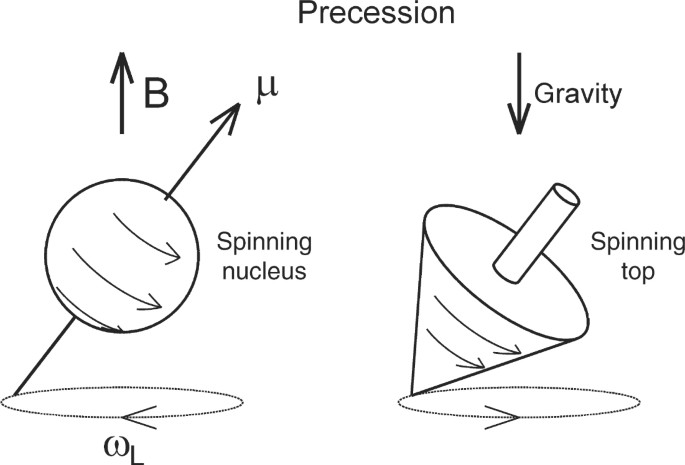
\includegraphics[width = 0.45 \textwidth]{figures/lamor.jpg}
    \caption{Left, model of Larmor precession of the nuclear spin about the direction of a steady applied magnetic field \textbf{B}. Right, analogous system a spinning top in a gravitational field.~\cite{Prasad2008}}
    \label{fig:lamor}
\end{figure}

  In the classical description of the resonance condition a rotating charge can be treated as a circulating current loop and as a result will have a magnetic dipole ($\mu$) described by $\mu = iA$, where `$i$' is the current and `$A$' is the cross-sectional area of the enclosed loop.~\cite{nmr65} However, as a proton is quantum object its magnetic moment is characterized by $\mu = \hbar \gamma \mathbf{I}$, where $\gamma$ is magnetogyric ratio and \textbf{I} is the magnetic quantum number given by nuclear spin.~\cite{nmr65}  When the a nucleon with magnetic moment $\mu$ is placed in a magnetic field the Hamiltonian for the system is given by

  \begin{gather}
    \mathscr{H} = -\mathbf{\mu}\cdot \mathbf{B} = -\hbar \gamma\mathbf{I}\cdot \mathbf{B} 
  \end{gather}
  with eigenvalues given by equation~\ref{eq:eigval}, ~\cite{nmr65}
  \begin{gather}
    E = \hbar \gamma m_z B_0 \label{eq:eigval}\\
    \Delta E = 2 \hbar \gamma m_z B_0 \label{eq:esplit}
  \end{gather}
  In the case of a proton $m_z = \pm 1/2$. This causes an energy split given by equation~\ref{eq:esplit} between the two levels as one state will align with the applied magnetic field while the other will be anti-aligned. Here m$_z$ are the projected values of \textbf{I} onto the z-axis defined by the magnetic field. 


  As this motion is akin to a harmonic oscillator we can set the energy difference equal to a characteristic, or in this case resonant frequency. The harmonic motion is the rotation or precession about the axis of the applied magnetic field. A toy model of this can be seen in figure~\ref{fig:lamor}. 

  \begin{gather}
    \Delta E_{proton} = \hbar \omega =  \hbar \gamma B_0 \nonumber \\
    \omega_0 = \gamma B_0 \rightarrow f_0 = \frac{\gamma B_0}{2 \pi}
  \end{gather}

  In properly address macroscopic samples we must define a net magnetization $\mathbf{M} = \sum_{i} \mu_i$. Now  we are able to look at a population of spins precessing about an applied magnetic field axis. However, the current model is only useful in a static equilibrium system, so in order to see the time evolution we can consider the system relaxing \textit{towards} equilibrium under the influence of an applied magentic field $\mathbf{B} = B_0 \hat{z}$ and solve the differential equation as shown by equations~\ref{eq:diff1}--\ref{eq:mzt1}.

\begin{gather}
    \mathbf{M}|_{\mathbf{B}} = M_0 \hat{z} \label{eq:diff1} \\
    \frac{dM_z}{dt} = \frac{M_0 - M_{z}}{T_1} \\
    M_z(t) = M_0 \left(1-2 e^\frac{-t}{T_1}\right) \label{eq:mzt1}
\end{gather}

  Here we took $M_z(t=0) = -M_0$, such that the initial magnetization vector pointed in the $-\hat{z}$-axis.This corresponds to complete anti-alignment with the applied field. Notice that we included a characteristic constant $T_1$, which is a characteristic constant that corresponds to the spin-lattice relaxation constant. This name comes from how the spins give the energy gained from the RF pulse to the surrounding lattice.~\cite{nmr65}

  The previous analysis fails to take into account the transverse magnetizations $M_x$ and $M_y$. This can be treated by solving the differential equation

  \begin{gather}
    \frac{dM_{i^*}}{dt} = \frac{M_0 - M_{i^*}}{T_2} \\
    \text{where } i = x , y
  \end{gather}


  Solving this system gives a simple exponential, with a characteristic time constant \tg that defines the spin-spin relaxation time constant. However, equation~\ref{eq:mzt2_wrong} is difficult to measure experimentally as there is some loss of the transverse magnetization due to stochastic fluctuations in the local nuclear fields. As a result the spin echo is typically measured instead (equation~\ref{eq:mzt2}). 

  \begin{gather}
    M_z(t) = M_0  e^\frac{-t}{T_2}  \label{eq:mzt2_wrong}\\
    M_z(t) = M_0  e^\frac{-2\tau}{T_2}  \label{eq:mzt2}
  \end{gather}

  The spin echo is related to how the spins dephase and rephase. Once the system is allowed to evolve the nuclear spins can precess in any direction as a result the measured signal is lost. If the spins are pulsed with a RF wave, they can be forced to realign themselves. This realignment and subsequent thermalization is the spin echo. In order to probe this various pulse sequences are used to coax the nuclear spins into behaving as desired.  

\subsection*{Pulse Sequences}


  Broad intro with applications thisi s a test of figure reference look at fig

  basics of physics i.e. nucelar spin and magnetic field alignment

\subsubsection*{T1 sequence}



\subsubsection*{spin echo}

\subsubsection*{CP method}

\subsubsection*{MG method}


\section*{Experimental }

\subsection*{Equipment}

    \begin{figure}[h]
      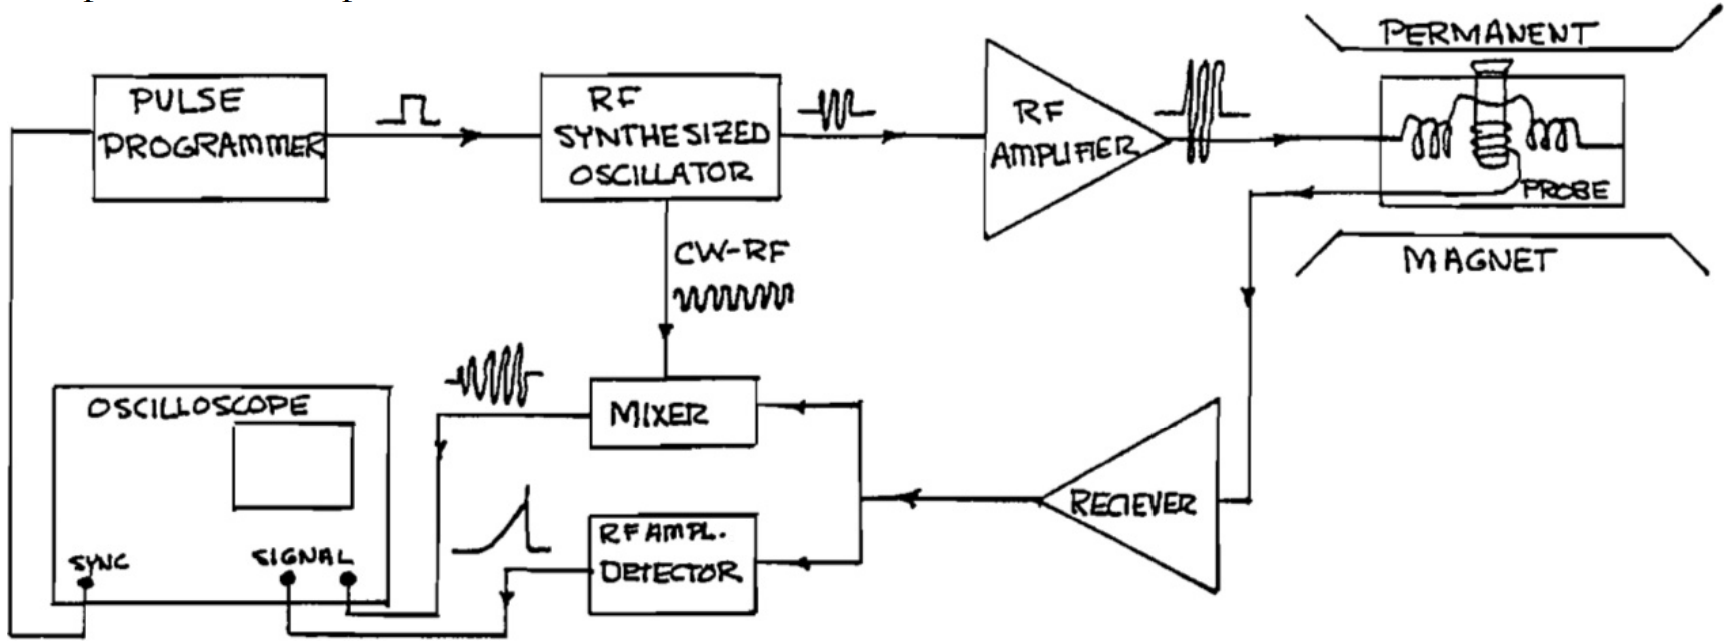
\includegraphics[width=0.4 \textwidth]{figures/block_diagram.png}
      \caption{Block diagram of experimental set up.}
      \label{fig:block}
    \end{figure}


    For these experiments, a TeachSpin PS1-A system was used to produce/amplify the pulse sequences, and pickup/amplify the output signal. The signal was then processed/synced and displayed on a Tektronix TBS 1052B Digital Oscilloscope. A simplified block diagram of the system is shown in figure~\ref{fig:block}. The pulse sequence begins at the \textbf{pulse programer}. The exact number of pulses, their widths, and time characteristics are defined in this module. This sends two signals, the first goes to the \textbf{oscilloscope}, the second to the \textbf{RF synthesized oscillator}. This first signal is to let the oscilloscope know when a output signal is coming. The second signal tells the RF synthesized oscillator what pulse sequence to generate. From there the pulse sequence is sent to an \textbf{RF amplifier} and the \textbf{mixer}. The amplifier ensure that a strong enough signal sequence is transmitted to the transmitter Helmholtz coils in the sample chamber such that it influences the nuclear spins. The mixer combines the reference signal with the sample output signal. Before getting to the mixer the sample output signal goes to the \textbf{receiver}. The receiver also sends the output signal to a \textbf{RF amplifier detector}. The mixer and RF amplifier detector both send the signal to the oscilloscope. 
    
    The \textbf{pulse programer} outputs pulses that are about 4V with a rise time of 15ns. The length of these pulses can be controlled with the A-width or B-width knobs and ranges from 1-30$\mu$s. The two knobs exists because it is able to program the number of pulses. Its capable of producing 1 A-pulse and between 0-99 B-pulses for a maximum of 100 pulses. It also can set the delay time ($\tau$) between pulses. This is done using the dial switches between the pulse width knobs.  If there are more than one B-pulses then the delay between the B-pulses is 2$\tau$. The repetition time knobs in the center of the module decide how long to wait before starting the next pulse train. 
    
    
  
    
    
    P1: block diagram and overview of set usepackage
    
    P2: 3module system

    p3: sample holder

    p4: oscilloscope


Discribe 3 module system,  oscilloscope. 


\subsection*{Procedure}

\subsubsection*{Sample Preparation} 
    The two chemical species of interest were mineral oil, and CuSO$_{4} \boldsymbol{\cdot} $H$_2$O. The mineral oil was used as purchased from supplier. As CuSO$_{4}$ is a blue crystalline solid it was dissolved in deionized water prior to measurement.Seven sample concentrations of 0.005M, 0.01M, 0.05M, 0.1M, 0.2M 0.5M, \& 1M \cuso were prepared. 

    Chemical species were loaded into their own glass sample vials. Samples should be approximately cubical (~5mm tall) so that the magnetic field is experienced uniformly in the entire sample. Sample vials are caped with a rubber stop to ensure that concentrations are consistent and there is minimal evaporation or contamination. A rubber o-ring was used to adjust the sample depth inside of the probe. The optimal depth maximizes the signal amplitude and is roughly 1.5 inches from the bottom of the sample vial. The o-ring was placed at the same height for all sample. 


\subsubsection*{Single pulse FID}
    
    The procedure used in this section are used for the rest of the sections as well, as the goal of this section is to get a spectra that is in resonance. It should be assumed that for all measurements after this that this section is repeated.

    In order to maximize signal output on the oscilloscope, the spectrometer receiver must be tuned. First the signal to noise ratio must be reasonable. There are two parameters that control this. The gain knob on the receiver was set to 50\%. Additionally, the time constant knob was set to 0.1ms, because above this point the signal amplitude decreased. From there the spectrometer was tuned using the tuning knob is located on the receiver. This knob turns a capacitor inside the receiver and should be rotated in such a way that the signal amplitude is maximized. These parameters are relatively consistent between samples however some minor tuning may be necessary.

    On the pulse programer the mode was set to int. Additionally, the repetition time is set to be long enough for the magnetization vector to return to its equilibrium position. In the case of mineral oil we set the repetition time to 500 ms. At this point, the pulse sequence needs to be programed. Each sequence is unique but the programming of them is procedurally the same. In the case of the one pulse free induction decay (FID) pulse sequence we have a single $90^\circ$ A-pulse. However, other sequences may have multiple pulses. In those cases you turn on the B-pulses as well, select the number of B-pulses and choose the desired B-pulse-angle in a similar manner to the A-pulse. 

    To find the desired pulse angle the A- or B-width knob is rotated clockwise starting from the zero point. For a $90^\circ$ pulse the signal amplitude will be at a maximum. On our instrument that was about 20\% of the way on. It is recommended that while finding the desired pulse length the other pulse is turned off and the sync is set to the pulse of interest. For example, if tuning the B-pulse to $90^\circ$ the A-pulse should be switched off, the sync should be on B and the number of pulses should be 1. This is so that no other factors influence the peak amplitude. The same is true when tuning the A-pulse; B-pulse should be off and sync set to A. 

    
    \begin{figure}
        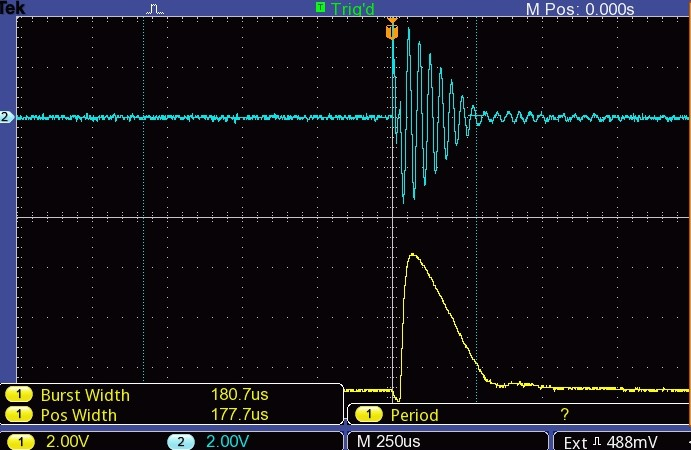
\includegraphics[width= 0.45\textwidth]{figures/noResonance.JPG}
        \caption{Single Pulse Free Induction Decay (FID) when out of resonance.}
        \label{fig:beats}
    \end{figure}

    As the magnet is $\sim 0.35$ Tesla, the resonant frequency will be around 15MHz. To find resonant frequency the frequency adjust knob is rotated until the mixer out spectra on the oscilloscope doesn't show any ``beats''. If the frequency is incorrect the displayed pulse will have multiple peaks within a single pulse, this is known as a beat (figure~\ref{fig:beats}). The resonance condition is when there is a single clean line that outlines a pulse or if it is perfectly flat. 

    Taking these parameters into account in order to acquire a single pulse FID of mineral oil the spectrometer must be set to output only the A-pulse, with a width of $\sim 20\%$, and a repetition time of 500m. From there a single clean pulse was found by tuning the frequency to 15.42707 MHz. A screenshot of the oscilloscope was taken. 

\subsubsection*{Magnetic Field Contours}

    In order to maximize signal amplitude the spatial dependence of the magnetic field was mapped so the sample can be placed in the section with the most uniform field. This was done by finding the resonant frequency at every point in a regular grid. Field uniformity is determined by a region with minimal change in the resonant frequency. Due to thermal effects the resonant frequency of the magnet drifts over time, thus  it is crucial to take these measurements rapidly. As the constant magnetic field $(B_0)$ was produced by a permanent ferromagnet, magnetic domain effects come into play. Some domains may be smaller than other and the most uniform field may not necessarily be in the center. However, it is also critical to avoid edge effects. 
    
    The direction of $B_0$ is parallel to the table top and will be called the z-axis. The sample holder allowed for freedom of movement in the x and y directions. Here the y-axis moved the sample up and down relative to table surface, while the x-direction moved the sample parallel to the surface but perpendicular to $B_0$. The values of the y-axis range from $0\ldots20~cm$ and begin at the bottom of the magnet and finish at the top. The x-axis places its zero point at the center of the magnet and ranges from $-10\ldots10~cm$. The field was mapped from $-1~cm \leq x \leq +1~cm$ with step sizes of $0.2~cm$ and from $9~cm \leq y \leq 11~cm$ with step sizes of $0.5~cm$. The resonance frequency values were mapped onto a contour plot and the section with the least change  in the resonant frequency was determined to have the most uniform magnetic field. 

\subsubsection*{Spin-Lattice Relaxation: T1 Sequence}


    A quick estimate of T$_1$ was acquired. First the spectrometer was set to resonance for a single pulse FID with a large repetition time. The repetition time was slowly lowered until the maximum amplitude of the FID decreased. The point just before the amplitude decrease is $\sim 4-5\times$T$_1$.

    For accurate measurement of T$_1$ a two pulse sequence of: $180^{\circ}- \tau \text{(variable)} - 90^{\circ}\text{ (FID)}$. An $180^{\circ}$ pulse is characterized by the amplitude of the pulse of interest being at a minimum, while a $90^{\circ}$ pulse is when the pulse amplitude is at a maximum as previously stated. So in this sequence the `A' pulse should be a minimum while the `B' pulse is maximized. However, if the sample is back in alignment with $B_0$ the signal received after the B-pulse will be unchanging. Thus by varying the delay time $(\tau )$ the amplitude of the B-pulse will vary until the saturation point is reached. By measuring the B-pulse amplitude over a range of delay times a fit can be made to equation~\ref{eq:mzt1}. \textbf{Note:} as the oscilloscope outputs the magnitude of the signal it will first appear as the signal is decreasing then increasing once it reaches zero see fig~\ref{fig:magnetization_t1}. Also for ease of measurement insure that pulse programer is synced to the B-pulse makes the measurement easier. 

    \begin{center}
        \begin{figure}[b]
            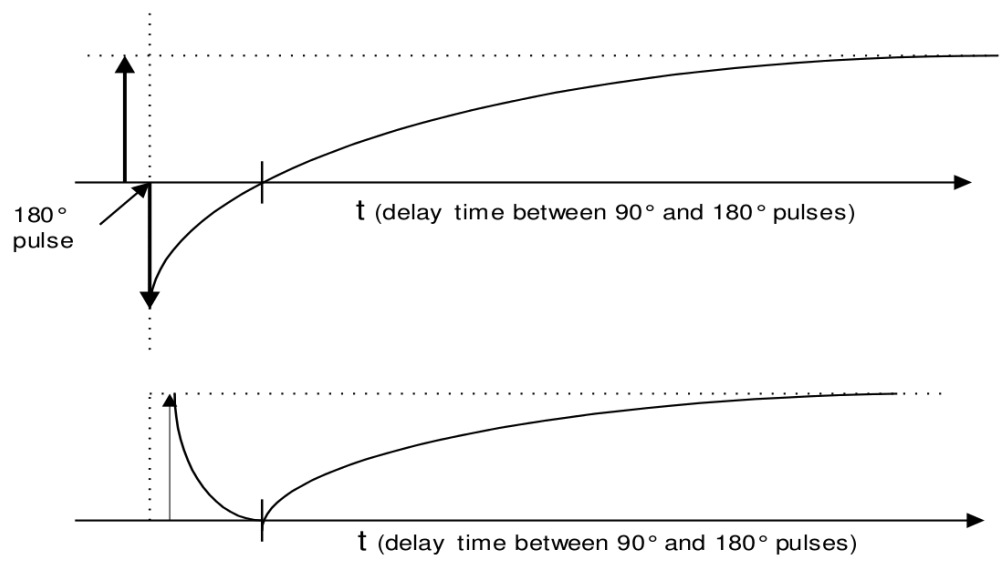
\includegraphics[width=0.4\textwidth]{figures/t1_pulse_magnetization.png}
            \caption{Top the z-component of the magnetization $(M_z)$vector over time. Bottom the amplitude of the magnetization.}
            \label{fig:magnetization_t1}
          \end{figure}
    \end{center}

\subsubsection*{Spin-Echo and Carl-Purcell methods}

    Both spin-echo and the Carl-Purcell method of measuring $T_2$ were only done on the mineral oil sample as the Meiboom-Gill pulse sequence is more accurate in nearly all cases.

    The spin-echo sequence is also a two pulse method however its sequence is: $90^{\circ}- \tau  - 180^{\circ}-\tau-\text{echo(at $2\tau$)}$. Similar to the $T_1$ measurement the signal amplitude decays as a function of the delay time. Thus the delay was varied by intervals of 10. The first two values were 1.5ms and 10ms and measurements ended at 90ms. The amplitudes were measured at varying delay times just like in the $T_1$ two-pulse method. A plot of delay time versus spin-echo amplitude was made and the $T_2$ was found by fitting equation~\ref{eq:mzt2}.

    The CP sequence is like the spin-echo method but with multiple B-pulses. Its sequence is: $90^{\circ}- \tau  - 180^{\circ}-2\tau- 180^{\circ}-2\tau- \dots$. Here the choice of delay time is critical as the spacing $2\tau$ should be short compared to the diffusion time of the spin through the magnetic field gradient. We used a delay time of 5 ms and 80 B-pulses for our measurements. The oscilloscope output was frozen and the spin-echo amplitude was measured at 10 points in intervals of $\sim$16 ms between peaks. Again the results were plotted and fitted to equation~\ref{eq:mzt2}.


    \begin{table}
    \begin{center}
    \begin{tabular}[t]{ |c|c|c| }
        \hline
        \multicolumn{3}{|c|}{Mineral Oil} \\ \hline 
        Molarity (mol/L) & Delay Time (ms) & Num. Pulses \\ \hline
        - & 4 & 60 \\ \hline 
    
        \multicolumn{3}{|c|}{CuSO$_{4} \boldsymbol{\cdot} $H$_2$O} \\ \hline
        Molarity (mol/L) & Delay Time (ms) & Num. Pulses \\ \hline
        0.005 M & 4 & 50 \\ \hline 
        0.01 M & 4 & 40  \\ \hline
        0.05 M & 1 & 50  \\ \hline 
        0.1 M & 0.8 & 50  \\ \hline
        0.2 M & 0.8 & 50  \\ \hline 
        0.5 M & 0.8 & 50  \\ \hline
        1.0 M & 0.1 & 20  \\ \hline 
    \end{tabular}
    \caption{The delay time and number of pulses used in the Meiboom-Gill pulse sequence for each mineral oil and \cuso. }
    \label{tab:delaytime}
    \end{center}
    \end{table}

\subsubsection*{Meiboom-Gill method}

    The MG method was used to find $T_2$ for the mineral oil and all the \cuso samples. This sequence is nearly identical to the CP sequence the only difference is that the $180^\circ$ pulses alternate in their direction; i.e. the sequence is $90^{\circ}- \tau  - 180^{\circ}-2\tau- ^{-}180^{\circ}-2\tau- 180^{\circ}\dots$. This is accomplished by turning on the MG switch on the pulse amplifier/mixer. The output signal was frozen on the oscilloscope monitor and 10--15 amplitudes were measured at regular time intervals. As the spin diffusion time is dependent on the chemical species and environment the optimal delay time and number of pulses changed between samples. Table~\ref{tab:delaytime} displays the values used in our lab. The results for each chemical species and concentration were plotted and fitted to equation~\ref{eq:mzt2}.


\section*{Results \lowercase{and} Discussion }

    The measured $T_1$ and $T_2$ values for both mineral oil and \cuso are summarized in table~\ref{tab:summery}. Additionally, detailed plots for all of the \cuso concentrations can be found in the Appendix. These sections will discuss the trends in the results with key examples.
  
\subsubsection*{Magnetic Field Contours}

  \begin{figure}[h]
    \resizebox{0.45\textwidth}{!}{%% Creator: Matplotlib, PGF backend
%%
%% To include the figure in your LaTeX document, write
%%   \input{<filename>.pgf}
%%
%% Make sure the required packages are loaded in your preamble
%%   \usepackage{pgf}
%%
%% Also ensure that all the required font packages are loaded; for instance,
%% the lmodern package is sometimes necessary when using math font.
%%   \usepackage{lmodern}
%%
%% Figures using additional raster images can only be included by \input if
%% they are in the same directory as the main LaTeX file. For loading figures
%% from other directories you can use the `import` package
%%   \usepackage{import}
%%
%% and then include the figures with
%%   \import{<path to file>}{<filename>.pgf}
%%
%% Matplotlib used the following preamble
%%   \usepackage{fontspec}
%%   \setmainfont{DejaVuSerif.ttf}[Path=\detokenize{/usr/share/matplotlib/mpl-data/fonts/ttf/}]
%%   \setsansfont{DejaVuSans.ttf}[Path=\detokenize{/usr/share/matplotlib/mpl-data/fonts/ttf/}]
%%   \setmonofont{DejaVuSansMono.ttf}[Path=\detokenize{/usr/share/matplotlib/mpl-data/fonts/ttf/}]
%%
\begingroup%
\makeatletter%
\begin{pgfpicture}%
\pgfpathrectangle{\pgfpointorigin}{\pgfqpoint{6.400000in}{4.800000in}}%
\pgfusepath{use as bounding box, clip}%
\begin{pgfscope}%
\pgfsetbuttcap%
\pgfsetmiterjoin%
\definecolor{currentfill}{rgb}{1.000000,1.000000,1.000000}%
\pgfsetfillcolor{currentfill}%
\pgfsetlinewidth{0.000000pt}%
\definecolor{currentstroke}{rgb}{1.000000,1.000000,1.000000}%
\pgfsetstrokecolor{currentstroke}%
\pgfsetdash{}{0pt}%
\pgfpathmoveto{\pgfqpoint{0.000000in}{0.000000in}}%
\pgfpathlineto{\pgfqpoint{6.400000in}{0.000000in}}%
\pgfpathlineto{\pgfqpoint{6.400000in}{4.800000in}}%
\pgfpathlineto{\pgfqpoint{0.000000in}{4.800000in}}%
\pgfpathlineto{\pgfqpoint{0.000000in}{0.000000in}}%
\pgfpathclose%
\pgfusepath{fill}%
\end{pgfscope}%
\begin{pgfscope}%
\pgfsetbuttcap%
\pgfsetmiterjoin%
\definecolor{currentfill}{rgb}{1.000000,1.000000,1.000000}%
\pgfsetfillcolor{currentfill}%
\pgfsetlinewidth{0.000000pt}%
\definecolor{currentstroke}{rgb}{0.000000,0.000000,0.000000}%
\pgfsetstrokecolor{currentstroke}%
\pgfsetstrokeopacity{0.000000}%
\pgfsetdash{}{0pt}%
\pgfpathmoveto{\pgfqpoint{1.485698in}{0.840429in}}%
\pgfpathlineto{\pgfqpoint{4.958681in}{0.840429in}}%
\pgfpathlineto{\pgfqpoint{4.958681in}{4.313411in}}%
\pgfpathlineto{\pgfqpoint{1.485698in}{4.313411in}}%
\pgfpathlineto{\pgfqpoint{1.485698in}{0.840429in}}%
\pgfpathclose%
\pgfusepath{fill}%
\end{pgfscope}%
\begin{pgfscope}%
\pgfpathrectangle{\pgfqpoint{1.485698in}{0.840429in}}{\pgfqpoint{3.472982in}{3.472982in}}%
\pgfusepath{clip}%
\pgfsetbuttcap%
\pgfsetroundjoin%
\definecolor{currentfill}{rgb}{0.020588,0.020588,0.028645}%
\pgfsetfillcolor{currentfill}%
\pgfsetlinewidth{0.000000pt}%
\definecolor{currentstroke}{rgb}{0.000000,0.000000,0.000000}%
\pgfsetstrokecolor{currentstroke}%
\pgfsetdash{}{0pt}%
\pgfpathmoveto{\pgfqpoint{4.958681in}{4.069795in}}%
\pgfpathlineto{\pgfqpoint{4.958681in}{4.313411in}}%
\pgfpathlineto{\pgfqpoint{4.717629in}{4.313411in}}%
\pgfpathlineto{\pgfqpoint{4.958681in}{4.069795in}}%
\pgfpathclose%
\pgfusepath{fill}%
\end{pgfscope}%
\begin{pgfscope}%
\pgfpathrectangle{\pgfqpoint{1.485698in}{0.840429in}}{\pgfqpoint{3.472982in}{3.472982in}}%
\pgfusepath{clip}%
\pgfsetbuttcap%
\pgfsetroundjoin%
\definecolor{currentfill}{rgb}{0.065196,0.065196,0.090708}%
\pgfsetfillcolor{currentfill}%
\pgfsetlinewidth{0.000000pt}%
\definecolor{currentstroke}{rgb}{0.000000,0.000000,0.000000}%
\pgfsetstrokecolor{currentstroke}%
\pgfsetdash{}{0pt}%
\pgfpathmoveto{\pgfqpoint{4.611382in}{4.004099in}}%
\pgfpathlineto{\pgfqpoint{4.958681in}{3.699174in}}%
\pgfpathlineto{\pgfqpoint{4.958681in}{4.069795in}}%
\pgfpathlineto{\pgfqpoint{4.717629in}{4.313411in}}%
\pgfpathlineto{\pgfqpoint{4.611382in}{4.313411in}}%
\pgfpathlineto{\pgfqpoint{4.428086in}{4.313411in}}%
\pgfpathlineto{\pgfqpoint{4.611382in}{4.004099in}}%
\pgfpathclose%
\pgfusepath{fill}%
\end{pgfscope}%
\begin{pgfscope}%
\pgfpathrectangle{\pgfqpoint{1.485698in}{0.840429in}}{\pgfqpoint{3.472982in}{3.472982in}}%
\pgfusepath{clip}%
\pgfsetbuttcap%
\pgfsetroundjoin%
\definecolor{currentfill}{rgb}{0.109804,0.109804,0.152771}%
\pgfsetfillcolor{currentfill}%
\pgfsetlinewidth{0.000000pt}%
\definecolor{currentstroke}{rgb}{0.000000,0.000000,0.000000}%
\pgfsetstrokecolor{currentstroke}%
\pgfsetdash{}{0pt}%
\pgfpathmoveto{\pgfqpoint{4.958681in}{2.478796in}}%
\pgfpathlineto{\pgfqpoint{4.958681in}{2.576920in}}%
\pgfpathlineto{\pgfqpoint{4.958681in}{3.445166in}}%
\pgfpathlineto{\pgfqpoint{4.958681in}{3.699174in}}%
\pgfpathlineto{\pgfqpoint{4.611382in}{4.004099in}}%
\pgfpathlineto{\pgfqpoint{4.428086in}{4.313411in}}%
\pgfpathlineto{\pgfqpoint{4.264084in}{4.313411in}}%
\pgfpathlineto{\pgfqpoint{4.212255in}{4.313411in}}%
\pgfpathlineto{\pgfqpoint{4.264084in}{4.137049in}}%
\pgfpathlineto{\pgfqpoint{4.611382in}{3.568620in}}%
\pgfpathlineto{\pgfqpoint{4.775987in}{3.445166in}}%
\pgfpathlineto{\pgfqpoint{4.835180in}{2.576920in}}%
\pgfpathlineto{\pgfqpoint{4.958681in}{2.478796in}}%
\pgfpathclose%
\pgfusepath{fill}%
\end{pgfscope}%
\begin{pgfscope}%
\pgfpathrectangle{\pgfqpoint{1.485698in}{0.840429in}}{\pgfqpoint{3.472982in}{3.472982in}}%
\pgfusepath{clip}%
\pgfsetbuttcap%
\pgfsetroundjoin%
\definecolor{currentfill}{rgb}{0.150980,0.150980,0.210060}%
\pgfsetfillcolor{currentfill}%
\pgfsetlinewidth{0.000000pt}%
\definecolor{currentstroke}{rgb}{0.000000,0.000000,0.000000}%
\pgfsetstrokecolor{currentstroke}%
\pgfsetdash{}{0pt}%
\pgfpathmoveto{\pgfqpoint{4.611382in}{2.561760in}}%
\pgfpathlineto{\pgfqpoint{4.958681in}{2.287901in}}%
\pgfpathlineto{\pgfqpoint{4.958681in}{2.478796in}}%
\pgfpathlineto{\pgfqpoint{4.835180in}{2.576920in}}%
\pgfpathlineto{\pgfqpoint{4.775987in}{3.445166in}}%
\pgfpathlineto{\pgfqpoint{4.611382in}{3.568620in}}%
\pgfpathlineto{\pgfqpoint{4.264084in}{4.137049in}}%
\pgfpathlineto{\pgfqpoint{4.212255in}{4.313411in}}%
\pgfpathlineto{\pgfqpoint{4.070058in}{4.313411in}}%
\pgfpathlineto{\pgfqpoint{4.264084in}{3.653183in}}%
\pgfpathlineto{\pgfqpoint{4.394321in}{3.445166in}}%
\pgfpathlineto{\pgfqpoint{4.588088in}{2.576920in}}%
\pgfpathlineto{\pgfqpoint{4.611382in}{2.561760in}}%
\pgfpathclose%
\pgfusepath{fill}%
\end{pgfscope}%
\begin{pgfscope}%
\pgfpathrectangle{\pgfqpoint{1.485698in}{0.840429in}}{\pgfqpoint{3.472982in}{3.472982in}}%
\pgfusepath{clip}%
\pgfsetbuttcap%
\pgfsetroundjoin%
\definecolor{currentfill}{rgb}{0.195588,0.195588,0.272123}%
\pgfsetfillcolor{currentfill}%
\pgfsetlinewidth{0.000000pt}%
\definecolor{currentstroke}{rgb}{0.000000,0.000000,0.000000}%
\pgfsetstrokecolor{currentstroke}%
\pgfsetdash{}{0pt}%
\pgfpathmoveto{\pgfqpoint{4.264084in}{2.565957in}}%
\pgfpathlineto{\pgfqpoint{4.611382in}{2.340564in}}%
\pgfpathlineto{\pgfqpoint{4.958681in}{2.097006in}}%
\pgfpathlineto{\pgfqpoint{4.958681in}{2.287901in}}%
\pgfpathlineto{\pgfqpoint{4.611382in}{2.561760in}}%
\pgfpathlineto{\pgfqpoint{4.588088in}{2.576920in}}%
\pgfpathlineto{\pgfqpoint{4.394321in}{3.445166in}}%
\pgfpathlineto{\pgfqpoint{4.264084in}{3.653183in}}%
\pgfpathlineto{\pgfqpoint{4.070058in}{4.313411in}}%
\pgfpathlineto{\pgfqpoint{3.927860in}{4.313411in}}%
\pgfpathlineto{\pgfqpoint{4.141862in}{3.445166in}}%
\pgfpathlineto{\pgfqpoint{4.251681in}{2.576920in}}%
\pgfpathlineto{\pgfqpoint{4.264084in}{2.565957in}}%
\pgfpathclose%
\pgfusepath{fill}%
\end{pgfscope}%
\begin{pgfscope}%
\pgfpathrectangle{\pgfqpoint{1.485698in}{0.840429in}}{\pgfqpoint{3.472982in}{3.472982in}}%
\pgfusepath{clip}%
\pgfsetbuttcap%
\pgfsetroundjoin%
\definecolor{currentfill}{rgb}{0.240196,0.240196,0.334186}%
\pgfsetfillcolor{currentfill}%
\pgfsetlinewidth{0.000000pt}%
\definecolor{currentstroke}{rgb}{0.000000,0.000000,0.000000}%
\pgfsetstrokecolor{currentstroke}%
\pgfsetdash{}{0pt}%
\pgfpathmoveto{\pgfqpoint{4.264084in}{2.331356in}}%
\pgfpathlineto{\pgfqpoint{4.611382in}{2.119368in}}%
\pgfpathlineto{\pgfqpoint{4.958681in}{1.906111in}}%
\pgfpathlineto{\pgfqpoint{4.958681in}{2.097006in}}%
\pgfpathlineto{\pgfqpoint{4.611382in}{2.340564in}}%
\pgfpathlineto{\pgfqpoint{4.264084in}{2.565957in}}%
\pgfpathlineto{\pgfqpoint{4.251681in}{2.576920in}}%
\pgfpathlineto{\pgfqpoint{4.141862in}{3.445166in}}%
\pgfpathlineto{\pgfqpoint{3.927860in}{4.313411in}}%
\pgfpathlineto{\pgfqpoint{3.916786in}{4.313411in}}%
\pgfpathlineto{\pgfqpoint{3.591469in}{4.313411in}}%
\pgfpathlineto{\pgfqpoint{3.916786in}{3.489690in}}%
\pgfpathlineto{\pgfqpoint{3.927472in}{3.445166in}}%
\pgfpathlineto{\pgfqpoint{3.986246in}{2.576920in}}%
\pgfpathlineto{\pgfqpoint{4.264084in}{2.331356in}}%
\pgfpathclose%
\pgfusepath{fill}%
\end{pgfscope}%
\begin{pgfscope}%
\pgfpathrectangle{\pgfqpoint{1.485698in}{0.840429in}}{\pgfqpoint{3.472982in}{3.472982in}}%
\pgfusepath{clip}%
\pgfsetbuttcap%
\pgfsetroundjoin%
\definecolor{currentfill}{rgb}{0.240196,0.240196,0.334186}%
\pgfsetfillcolor{currentfill}%
\pgfsetlinewidth{0.000000pt}%
\definecolor{currentstroke}{rgb}{0.000000,0.000000,0.000000}%
\pgfsetstrokecolor{currentstroke}%
\pgfsetdash{}{0pt}%
\pgfpathmoveto{\pgfqpoint{1.522432in}{4.313411in}}%
\pgfpathlineto{\pgfqpoint{1.485698in}{4.313411in}}%
\pgfpathlineto{\pgfqpoint{1.485698in}{4.304527in}}%
\pgfpathlineto{\pgfqpoint{1.522432in}{4.313411in}}%
\pgfpathclose%
\pgfusepath{fill}%
\end{pgfscope}%
\begin{pgfscope}%
\pgfpathrectangle{\pgfqpoint{1.485698in}{0.840429in}}{\pgfqpoint{3.472982in}{3.472982in}}%
\pgfusepath{clip}%
\pgfsetbuttcap%
\pgfsetroundjoin%
\definecolor{currentfill}{rgb}{0.284804,0.284804,0.396249}%
\pgfsetfillcolor{currentfill}%
\pgfsetlinewidth{0.000000pt}%
\definecolor{currentstroke}{rgb}{0.000000,0.000000,0.000000}%
\pgfsetstrokecolor{currentstroke}%
\pgfsetdash{}{0pt}%
\pgfpathmoveto{\pgfqpoint{4.958681in}{0.840429in}}%
\pgfpathlineto{\pgfqpoint{4.958681in}{1.657875in}}%
\pgfpathlineto{\pgfqpoint{4.771266in}{0.840429in}}%
\pgfpathlineto{\pgfqpoint{4.958681in}{0.840429in}}%
\pgfpathclose%
\pgfusepath{fill}%
\end{pgfscope}%
\begin{pgfscope}%
\pgfpathrectangle{\pgfqpoint{1.485698in}{0.840429in}}{\pgfqpoint{3.472982in}{3.472982in}}%
\pgfusepath{clip}%
\pgfsetbuttcap%
\pgfsetroundjoin%
\definecolor{currentfill}{rgb}{0.284804,0.284804,0.396249}%
\pgfsetfillcolor{currentfill}%
\pgfsetlinewidth{0.000000pt}%
\definecolor{currentstroke}{rgb}{0.000000,0.000000,0.000000}%
\pgfsetstrokecolor{currentstroke}%
\pgfsetdash{}{0pt}%
\pgfpathmoveto{\pgfqpoint{3.916786in}{2.370320in}}%
\pgfpathlineto{\pgfqpoint{4.264084in}{2.096754in}}%
\pgfpathlineto{\pgfqpoint{4.611382in}{1.898173in}}%
\pgfpathlineto{\pgfqpoint{4.958681in}{1.715216in}}%
\pgfpathlineto{\pgfqpoint{4.958681in}{1.906111in}}%
\pgfpathlineto{\pgfqpoint{4.611382in}{2.119368in}}%
\pgfpathlineto{\pgfqpoint{4.264084in}{2.331356in}}%
\pgfpathlineto{\pgfqpoint{3.986246in}{2.576920in}}%
\pgfpathlineto{\pgfqpoint{3.927472in}{3.445166in}}%
\pgfpathlineto{\pgfqpoint{3.916786in}{3.489690in}}%
\pgfpathlineto{\pgfqpoint{3.591469in}{4.313411in}}%
\pgfpathlineto{\pgfqpoint{3.569488in}{4.313411in}}%
\pgfpathlineto{\pgfqpoint{3.222190in}{4.313411in}}%
\pgfpathlineto{\pgfqpoint{3.101820in}{4.313411in}}%
\pgfpathlineto{\pgfqpoint{3.222190in}{4.118695in}}%
\pgfpathlineto{\pgfqpoint{3.569488in}{3.553697in}}%
\pgfpathlineto{\pgfqpoint{3.612401in}{3.445166in}}%
\pgfpathlineto{\pgfqpoint{3.822825in}{2.576920in}}%
\pgfpathlineto{\pgfqpoint{3.916786in}{2.370320in}}%
\pgfpathclose%
\pgfusepath{fill}%
\end{pgfscope}%
\begin{pgfscope}%
\pgfpathrectangle{\pgfqpoint{1.485698in}{0.840429in}}{\pgfqpoint{3.472982in}{3.472982in}}%
\pgfusepath{clip}%
\pgfsetbuttcap%
\pgfsetroundjoin%
\definecolor{currentfill}{rgb}{0.284804,0.284804,0.396249}%
\pgfsetfillcolor{currentfill}%
\pgfsetlinewidth{0.000000pt}%
\definecolor{currentstroke}{rgb}{0.000000,0.000000,0.000000}%
\pgfsetstrokecolor{currentstroke}%
\pgfsetdash{}{0pt}%
\pgfpathmoveto{\pgfqpoint{1.790419in}{4.313411in}}%
\pgfpathlineto{\pgfqpoint{1.522432in}{4.313411in}}%
\pgfpathlineto{\pgfqpoint{1.485698in}{4.304527in}}%
\pgfpathlineto{\pgfqpoint{1.485698in}{4.239712in}}%
\pgfpathlineto{\pgfqpoint{1.790419in}{4.313411in}}%
\pgfpathclose%
\pgfusepath{fill}%
\end{pgfscope}%
\begin{pgfscope}%
\pgfpathrectangle{\pgfqpoint{1.485698in}{0.840429in}}{\pgfqpoint{3.472982in}{3.472982in}}%
\pgfusepath{clip}%
\pgfsetbuttcap%
\pgfsetroundjoin%
\definecolor{currentfill}{rgb}{0.329412,0.333150,0.454412}%
\pgfsetfillcolor{currentfill}%
\pgfsetlinewidth{0.000000pt}%
\definecolor{currentstroke}{rgb}{0.000000,0.000000,0.000000}%
\pgfsetstrokecolor{currentstroke}%
\pgfsetdash{}{0pt}%
\pgfpathmoveto{\pgfqpoint{4.611382in}{0.840429in}}%
\pgfpathlineto{\pgfqpoint{4.771266in}{0.840429in}}%
\pgfpathlineto{\pgfqpoint{4.958681in}{1.657875in}}%
\pgfpathlineto{\pgfqpoint{4.958681in}{1.708675in}}%
\pgfpathlineto{\pgfqpoint{4.958681in}{1.715216in}}%
\pgfpathlineto{\pgfqpoint{4.611382in}{1.898173in}}%
\pgfpathlineto{\pgfqpoint{4.264084in}{2.096754in}}%
\pgfpathlineto{\pgfqpoint{3.916786in}{2.370320in}}%
\pgfpathlineto{\pgfqpoint{3.822825in}{2.576920in}}%
\pgfpathlineto{\pgfqpoint{3.612401in}{3.445166in}}%
\pgfpathlineto{\pgfqpoint{3.569488in}{3.553697in}}%
\pgfpathlineto{\pgfqpoint{3.222190in}{4.118695in}}%
\pgfpathlineto{\pgfqpoint{3.101820in}{4.313411in}}%
\pgfpathlineto{\pgfqpoint{2.874891in}{4.313411in}}%
\pgfpathlineto{\pgfqpoint{2.527593in}{4.313411in}}%
\pgfpathlineto{\pgfqpoint{2.180295in}{4.313411in}}%
\pgfpathlineto{\pgfqpoint{1.832997in}{4.313411in}}%
\pgfpathlineto{\pgfqpoint{1.790419in}{4.313411in}}%
\pgfpathlineto{\pgfqpoint{1.485698in}{4.239712in}}%
\pgfpathlineto{\pgfqpoint{1.485698in}{4.174896in}}%
\pgfpathlineto{\pgfqpoint{1.819156in}{3.445166in}}%
\pgfpathlineto{\pgfqpoint{1.832997in}{3.290122in}}%
\pgfpathlineto{\pgfqpoint{2.180295in}{3.274039in}}%
\pgfpathlineto{\pgfqpoint{2.527593in}{3.343494in}}%
\pgfpathlineto{\pgfqpoint{2.776227in}{3.445166in}}%
\pgfpathlineto{\pgfqpoint{2.874891in}{3.614745in}}%
\pgfpathlineto{\pgfqpoint{2.983422in}{3.445166in}}%
\pgfpathlineto{\pgfqpoint{3.222190in}{3.309502in}}%
\pgfpathlineto{\pgfqpoint{3.569488in}{3.040179in}}%
\pgfpathlineto{\pgfqpoint{3.695562in}{2.576920in}}%
\pgfpathlineto{\pgfqpoint{3.916786in}{2.090494in}}%
\pgfpathlineto{\pgfqpoint{4.264084in}{1.862153in}}%
\pgfpathlineto{\pgfqpoint{4.548977in}{1.708675in}}%
\pgfpathlineto{\pgfqpoint{4.474714in}{0.840429in}}%
\pgfpathlineto{\pgfqpoint{4.611382in}{0.840429in}}%
\pgfpathclose%
\pgfusepath{fill}%
\end{pgfscope}%
\begin{pgfscope}%
\pgfpathrectangle{\pgfqpoint{1.485698in}{0.840429in}}{\pgfqpoint{3.472982in}{3.472982in}}%
\pgfusepath{clip}%
\pgfsetbuttcap%
\pgfsetroundjoin%
\definecolor{currentfill}{rgb}{0.370588,0.389767,0.495588}%
\pgfsetfillcolor{currentfill}%
\pgfsetlinewidth{0.000000pt}%
\definecolor{currentstroke}{rgb}{0.000000,0.000000,0.000000}%
\pgfsetstrokecolor{currentstroke}%
\pgfsetdash{}{0pt}%
\pgfpathmoveto{\pgfqpoint{4.264084in}{0.840429in}}%
\pgfpathlineto{\pgfqpoint{4.474714in}{0.840429in}}%
\pgfpathlineto{\pgfqpoint{4.548977in}{1.708675in}}%
\pgfpathlineto{\pgfqpoint{4.264084in}{1.862153in}}%
\pgfpathlineto{\pgfqpoint{3.916786in}{2.090494in}}%
\pgfpathlineto{\pgfqpoint{3.695562in}{2.576920in}}%
\pgfpathlineto{\pgfqpoint{3.569488in}{3.040179in}}%
\pgfpathlineto{\pgfqpoint{3.222190in}{3.309502in}}%
\pgfpathlineto{\pgfqpoint{2.983422in}{3.445166in}}%
\pgfpathlineto{\pgfqpoint{2.874891in}{3.614745in}}%
\pgfpathlineto{\pgfqpoint{2.776227in}{3.445166in}}%
\pgfpathlineto{\pgfqpoint{2.527593in}{3.343494in}}%
\pgfpathlineto{\pgfqpoint{2.180295in}{3.274039in}}%
\pgfpathlineto{\pgfqpoint{1.832997in}{3.290122in}}%
\pgfpathlineto{\pgfqpoint{1.819156in}{3.445166in}}%
\pgfpathlineto{\pgfqpoint{1.485698in}{4.174896in}}%
\pgfpathlineto{\pgfqpoint{1.485698in}{4.110080in}}%
\pgfpathlineto{\pgfqpoint{1.789538in}{3.445166in}}%
\pgfpathlineto{\pgfqpoint{1.832997in}{2.958328in}}%
\pgfpathlineto{\pgfqpoint{2.180295in}{2.984923in}}%
\pgfpathlineto{\pgfqpoint{2.527593in}{3.084473in}}%
\pgfpathlineto{\pgfqpoint{2.874891in}{3.133930in}}%
\pgfpathlineto{\pgfqpoint{3.222190in}{2.913612in}}%
\pgfpathlineto{\pgfqpoint{3.565713in}{2.576920in}}%
\pgfpathlineto{\pgfqpoint{3.569488in}{2.573863in}}%
\pgfpathlineto{\pgfqpoint{3.916786in}{1.810668in}}%
\pgfpathlineto{\pgfqpoint{4.095005in}{1.708675in}}%
\pgfpathlineto{\pgfqpoint{4.218346in}{0.840429in}}%
\pgfpathlineto{\pgfqpoint{4.264084in}{0.840429in}}%
\pgfpathclose%
\pgfusepath{fill}%
\end{pgfscope}%
\begin{pgfscope}%
\pgfpathrectangle{\pgfqpoint{1.485698in}{0.840429in}}{\pgfqpoint{3.472982in}{3.472982in}}%
\pgfusepath{clip}%
\pgfsetbuttcap%
\pgfsetroundjoin%
\definecolor{currentfill}{rgb}{0.415196,0.451103,0.540196}%
\pgfsetfillcolor{currentfill}%
\pgfsetlinewidth{0.000000pt}%
\definecolor{currentstroke}{rgb}{0.000000,0.000000,0.000000}%
\pgfsetstrokecolor{currentstroke}%
\pgfsetdash{}{0pt}%
\pgfpathmoveto{\pgfqpoint{1.521626in}{1.708675in}}%
\pgfpathlineto{\pgfqpoint{1.535314in}{2.576920in}}%
\pgfpathlineto{\pgfqpoint{1.485698in}{2.579251in}}%
\pgfpathlineto{\pgfqpoint{1.485698in}{2.576920in}}%
\pgfpathlineto{\pgfqpoint{1.485698in}{1.708675in}}%
\pgfpathlineto{\pgfqpoint{1.485698in}{1.689890in}}%
\pgfpathlineto{\pgfqpoint{1.521626in}{1.708675in}}%
\pgfpathclose%
\pgfusepath{fill}%
\end{pgfscope}%
\begin{pgfscope}%
\pgfpathrectangle{\pgfqpoint{1.485698in}{0.840429in}}{\pgfqpoint{3.472982in}{3.472982in}}%
\pgfusepath{clip}%
\pgfsetbuttcap%
\pgfsetroundjoin%
\definecolor{currentfill}{rgb}{0.415196,0.451103,0.540196}%
\pgfsetfillcolor{currentfill}%
\pgfsetlinewidth{0.000000pt}%
\definecolor{currentstroke}{rgb}{0.000000,0.000000,0.000000}%
\pgfsetstrokecolor{currentstroke}%
\pgfsetdash{}{0pt}%
\pgfpathmoveto{\pgfqpoint{3.916786in}{1.057490in}}%
\pgfpathlineto{\pgfqpoint{3.969501in}{0.840429in}}%
\pgfpathlineto{\pgfqpoint{4.218346in}{0.840429in}}%
\pgfpathlineto{\pgfqpoint{4.095005in}{1.708675in}}%
\pgfpathlineto{\pgfqpoint{3.916786in}{1.810668in}}%
\pgfpathlineto{\pgfqpoint{3.569488in}{2.573863in}}%
\pgfpathlineto{\pgfqpoint{3.565713in}{2.576920in}}%
\pgfpathlineto{\pgfqpoint{3.222190in}{2.913612in}}%
\pgfpathlineto{\pgfqpoint{2.874891in}{3.133930in}}%
\pgfpathlineto{\pgfqpoint{2.527593in}{3.084473in}}%
\pgfpathlineto{\pgfqpoint{2.180295in}{2.984923in}}%
\pgfpathlineto{\pgfqpoint{1.832997in}{2.958328in}}%
\pgfpathlineto{\pgfqpoint{1.789538in}{3.445166in}}%
\pgfpathlineto{\pgfqpoint{1.485698in}{4.110080in}}%
\pgfpathlineto{\pgfqpoint{1.485698in}{4.045265in}}%
\pgfpathlineto{\pgfqpoint{1.759920in}{3.445166in}}%
\pgfpathlineto{\pgfqpoint{1.832997in}{2.626534in}}%
\pgfpathlineto{\pgfqpoint{2.180295in}{2.695808in}}%
\pgfpathlineto{\pgfqpoint{2.527593in}{2.825451in}}%
\pgfpathlineto{\pgfqpoint{2.874891in}{2.765270in}}%
\pgfpathlineto{\pgfqpoint{3.143556in}{2.576920in}}%
\pgfpathlineto{\pgfqpoint{3.222190in}{2.524564in}}%
\pgfpathlineto{\pgfqpoint{3.569488in}{2.246742in}}%
\pgfpathlineto{\pgfqpoint{3.819998in}{1.708675in}}%
\pgfpathlineto{\pgfqpoint{3.916786in}{1.057490in}}%
\pgfpathclose%
\pgfusepath{fill}%
\end{pgfscope}%
\begin{pgfscope}%
\pgfpathrectangle{\pgfqpoint{1.485698in}{0.840429in}}{\pgfqpoint{3.472982in}{3.472982in}}%
\pgfusepath{clip}%
\pgfsetbuttcap%
\pgfsetroundjoin%
\definecolor{currentfill}{rgb}{0.459804,0.512439,0.584804}%
\pgfsetfillcolor{currentfill}%
\pgfsetlinewidth{0.000000pt}%
\definecolor{currentstroke}{rgb}{0.000000,0.000000,0.000000}%
\pgfsetstrokecolor{currentstroke}%
\pgfsetdash{}{0pt}%
\pgfpathmoveto{\pgfqpoint{1.832997in}{1.703337in}}%
\pgfpathlineto{\pgfqpoint{1.843850in}{1.708675in}}%
\pgfpathlineto{\pgfqpoint{2.180295in}{2.226282in}}%
\pgfpathlineto{\pgfqpoint{2.527593in}{2.560418in}}%
\pgfpathlineto{\pgfqpoint{2.874891in}{2.269905in}}%
\pgfpathlineto{\pgfqpoint{3.222190in}{2.174429in}}%
\pgfpathlineto{\pgfqpoint{3.569488in}{1.919622in}}%
\pgfpathlineto{\pgfqpoint{3.667699in}{1.708675in}}%
\pgfpathlineto{\pgfqpoint{3.703518in}{0.840429in}}%
\pgfpathlineto{\pgfqpoint{3.916786in}{0.840429in}}%
\pgfpathlineto{\pgfqpoint{3.969501in}{0.840429in}}%
\pgfpathlineto{\pgfqpoint{3.916786in}{1.057490in}}%
\pgfpathlineto{\pgfqpoint{3.819998in}{1.708675in}}%
\pgfpathlineto{\pgfqpoint{3.569488in}{2.246742in}}%
\pgfpathlineto{\pgfqpoint{3.222190in}{2.524564in}}%
\pgfpathlineto{\pgfqpoint{3.143556in}{2.576920in}}%
\pgfpathlineto{\pgfqpoint{2.874891in}{2.765270in}}%
\pgfpathlineto{\pgfqpoint{2.527593in}{2.825451in}}%
\pgfpathlineto{\pgfqpoint{2.180295in}{2.695808in}}%
\pgfpathlineto{\pgfqpoint{1.832997in}{2.626534in}}%
\pgfpathlineto{\pgfqpoint{1.759920in}{3.445166in}}%
\pgfpathlineto{\pgfqpoint{1.485698in}{4.045265in}}%
\pgfpathlineto{\pgfqpoint{1.485698in}{3.980449in}}%
\pgfpathlineto{\pgfqpoint{1.730302in}{3.445166in}}%
\pgfpathlineto{\pgfqpoint{1.485698in}{2.672777in}}%
\pgfpathlineto{\pgfqpoint{1.485698in}{2.579251in}}%
\pgfpathlineto{\pgfqpoint{1.535314in}{2.576920in}}%
\pgfpathlineto{\pgfqpoint{1.521626in}{1.708675in}}%
\pgfpathlineto{\pgfqpoint{1.485698in}{1.689890in}}%
\pgfpathlineto{\pgfqpoint{1.485698in}{1.522398in}}%
\pgfpathlineto{\pgfqpoint{1.832997in}{1.703337in}}%
\pgfpathclose%
\pgfusepath{fill}%
\end{pgfscope}%
\begin{pgfscope}%
\pgfpathrectangle{\pgfqpoint{1.485698in}{0.840429in}}{\pgfqpoint{3.472982in}{3.472982in}}%
\pgfusepath{clip}%
\pgfsetbuttcap%
\pgfsetroundjoin%
\definecolor{currentfill}{rgb}{0.504412,0.573774,0.629412}%
\pgfsetfillcolor{currentfill}%
\pgfsetlinewidth{0.000000pt}%
\definecolor{currentstroke}{rgb}{0.000000,0.000000,0.000000}%
\pgfsetstrokecolor{currentstroke}%
\pgfsetdash{}{0pt}%
\pgfpathmoveto{\pgfqpoint{1.832997in}{1.512964in}}%
\pgfpathlineto{\pgfqpoint{2.180295in}{1.677020in}}%
\pgfpathlineto{\pgfqpoint{2.217505in}{1.708675in}}%
\pgfpathlineto{\pgfqpoint{2.527593in}{2.152952in}}%
\pgfpathlineto{\pgfqpoint{2.844141in}{1.708675in}}%
\pgfpathlineto{\pgfqpoint{2.874891in}{1.667213in}}%
\pgfpathlineto{\pgfqpoint{2.959236in}{1.708675in}}%
\pgfpathlineto{\pgfqpoint{3.222190in}{1.824295in}}%
\pgfpathlineto{\pgfqpoint{3.389524in}{1.708675in}}%
\pgfpathlineto{\pgfqpoint{3.520135in}{0.840429in}}%
\pgfpathlineto{\pgfqpoint{3.569488in}{0.840429in}}%
\pgfpathlineto{\pgfqpoint{3.703518in}{0.840429in}}%
\pgfpathlineto{\pgfqpoint{3.667699in}{1.708675in}}%
\pgfpathlineto{\pgfqpoint{3.569488in}{1.919622in}}%
\pgfpathlineto{\pgfqpoint{3.222190in}{2.174429in}}%
\pgfpathlineto{\pgfqpoint{2.874891in}{2.269905in}}%
\pgfpathlineto{\pgfqpoint{2.527593in}{2.560418in}}%
\pgfpathlineto{\pgfqpoint{2.180295in}{2.226282in}}%
\pgfpathlineto{\pgfqpoint{1.843850in}{1.708675in}}%
\pgfpathlineto{\pgfqpoint{1.832997in}{1.703337in}}%
\pgfpathlineto{\pgfqpoint{1.485698in}{1.522398in}}%
\pgfpathlineto{\pgfqpoint{1.485698in}{1.354906in}}%
\pgfpathlineto{\pgfqpoint{1.832997in}{1.512964in}}%
\pgfpathclose%
\pgfusepath{fill}%
\end{pgfscope}%
\begin{pgfscope}%
\pgfpathrectangle{\pgfqpoint{1.485698in}{0.840429in}}{\pgfqpoint{3.472982in}{3.472982in}}%
\pgfusepath{clip}%
\pgfsetbuttcap%
\pgfsetroundjoin%
\definecolor{currentfill}{rgb}{0.504412,0.573774,0.629412}%
\pgfsetfillcolor{currentfill}%
\pgfsetlinewidth{0.000000pt}%
\definecolor{currentstroke}{rgb}{0.000000,0.000000,0.000000}%
\pgfsetstrokecolor{currentstroke}%
\pgfsetdash{}{0pt}%
\pgfpathmoveto{\pgfqpoint{2.527593in}{0.840429in}}%
\pgfpathlineto{\pgfqpoint{2.616703in}{0.840429in}}%
\pgfpathlineto{\pgfqpoint{2.527593in}{1.188322in}}%
\pgfpathlineto{\pgfqpoint{2.467126in}{0.840429in}}%
\pgfpathlineto{\pgfqpoint{2.527593in}{0.840429in}}%
\pgfpathclose%
\pgfusepath{fill}%
\end{pgfscope}%
\begin{pgfscope}%
\pgfpathrectangle{\pgfqpoint{1.485698in}{0.840429in}}{\pgfqpoint{3.472982in}{3.472982in}}%
\pgfusepath{clip}%
\pgfsetbuttcap%
\pgfsetroundjoin%
\definecolor{currentfill}{rgb}{0.504412,0.573774,0.629412}%
\pgfsetfillcolor{currentfill}%
\pgfsetlinewidth{0.000000pt}%
\definecolor{currentstroke}{rgb}{0.000000,0.000000,0.000000}%
\pgfsetstrokecolor{currentstroke}%
\pgfsetdash{}{0pt}%
\pgfpathmoveto{\pgfqpoint{1.730302in}{3.445166in}}%
\pgfpathlineto{\pgfqpoint{1.485698in}{3.980449in}}%
\pgfpathlineto{\pgfqpoint{1.485698in}{3.915634in}}%
\pgfpathlineto{\pgfqpoint{1.700684in}{3.445166in}}%
\pgfpathlineto{\pgfqpoint{1.485698in}{2.766303in}}%
\pgfpathlineto{\pgfqpoint{1.485698in}{2.672777in}}%
\pgfpathlineto{\pgfqpoint{1.730302in}{3.445166in}}%
\pgfpathclose%
\pgfusepath{fill}%
\end{pgfscope}%
\begin{pgfscope}%
\pgfpathrectangle{\pgfqpoint{1.485698in}{0.840429in}}{\pgfqpoint{3.472982in}{3.472982in}}%
\pgfusepath{clip}%
\pgfsetbuttcap%
\pgfsetroundjoin%
\definecolor{currentfill}{rgb}{0.549020,0.635110,0.674020}%
\pgfsetfillcolor{currentfill}%
\pgfsetlinewidth{0.000000pt}%
\definecolor{currentstroke}{rgb}{0.000000,0.000000,0.000000}%
\pgfsetstrokecolor{currentstroke}%
\pgfsetdash{}{0pt}%
\pgfpathmoveto{\pgfqpoint{1.832997in}{1.322590in}}%
\pgfpathlineto{\pgfqpoint{2.180295in}{1.435087in}}%
\pgfpathlineto{\pgfqpoint{2.384178in}{0.840429in}}%
\pgfpathlineto{\pgfqpoint{2.467126in}{0.840429in}}%
\pgfpathlineto{\pgfqpoint{2.527593in}{1.188322in}}%
\pgfpathlineto{\pgfqpoint{2.616703in}{0.840429in}}%
\pgfpathlineto{\pgfqpoint{2.738942in}{0.840429in}}%
\pgfpathlineto{\pgfqpoint{2.874891in}{1.275771in}}%
\pgfpathlineto{\pgfqpoint{3.222190in}{1.494600in}}%
\pgfpathlineto{\pgfqpoint{3.422343in}{0.840429in}}%
\pgfpathlineto{\pgfqpoint{3.520135in}{0.840429in}}%
\pgfpathlineto{\pgfqpoint{3.389524in}{1.708675in}}%
\pgfpathlineto{\pgfqpoint{3.222190in}{1.824295in}}%
\pgfpathlineto{\pgfqpoint{2.959236in}{1.708675in}}%
\pgfpathlineto{\pgfqpoint{2.874891in}{1.667213in}}%
\pgfpathlineto{\pgfqpoint{2.844141in}{1.708675in}}%
\pgfpathlineto{\pgfqpoint{2.527593in}{2.152952in}}%
\pgfpathlineto{\pgfqpoint{2.217505in}{1.708675in}}%
\pgfpathlineto{\pgfqpoint{2.180295in}{1.677020in}}%
\pgfpathlineto{\pgfqpoint{1.832997in}{1.512964in}}%
\pgfpathlineto{\pgfqpoint{1.485698in}{1.354906in}}%
\pgfpathlineto{\pgfqpoint{1.485698in}{1.187414in}}%
\pgfpathlineto{\pgfqpoint{1.832997in}{1.322590in}}%
\pgfpathclose%
\pgfpathmoveto{\pgfqpoint{2.501900in}{1.708675in}}%
\pgfpathlineto{\pgfqpoint{2.527593in}{1.745487in}}%
\pgfpathlineto{\pgfqpoint{2.553822in}{1.708675in}}%
\pgfpathlineto{\pgfqpoint{2.527593in}{1.665560in}}%
\pgfpathlineto{\pgfqpoint{2.501900in}{1.708675in}}%
\pgfpathclose%
\pgfusepath{fill}%
\end{pgfscope}%
\begin{pgfscope}%
\pgfpathrectangle{\pgfqpoint{1.485698in}{0.840429in}}{\pgfqpoint{3.472982in}{3.472982in}}%
\pgfusepath{clip}%
\pgfsetbuttcap%
\pgfsetroundjoin%
\definecolor{currentfill}{rgb}{0.549020,0.635110,0.674020}%
\pgfsetfillcolor{currentfill}%
\pgfsetlinewidth{0.000000pt}%
\definecolor{currentstroke}{rgb}{0.000000,0.000000,0.000000}%
\pgfsetstrokecolor{currentstroke}%
\pgfsetdash{}{0pt}%
\pgfpathmoveto{\pgfqpoint{1.700684in}{3.445166in}}%
\pgfpathlineto{\pgfqpoint{1.485698in}{3.915634in}}%
\pgfpathlineto{\pgfqpoint{1.485698in}{3.850818in}}%
\pgfpathlineto{\pgfqpoint{1.671066in}{3.445166in}}%
\pgfpathlineto{\pgfqpoint{1.485698in}{2.859829in}}%
\pgfpathlineto{\pgfqpoint{1.485698in}{2.766303in}}%
\pgfpathlineto{\pgfqpoint{1.700684in}{3.445166in}}%
\pgfpathclose%
\pgfusepath{fill}%
\end{pgfscope}%
\begin{pgfscope}%
\pgfpathrectangle{\pgfqpoint{1.485698in}{0.840429in}}{\pgfqpoint{3.472982in}{3.472982in}}%
\pgfusepath{clip}%
\pgfsetbuttcap%
\pgfsetroundjoin%
\definecolor{currentfill}{rgb}{0.590196,0.691728,0.715196}%
\pgfsetfillcolor{currentfill}%
\pgfsetlinewidth{0.000000pt}%
\definecolor{currentstroke}{rgb}{0.000000,0.000000,0.000000}%
\pgfsetstrokecolor{currentstroke}%
\pgfsetdash{}{0pt}%
\pgfpathmoveto{\pgfqpoint{1.832997in}{1.132217in}}%
\pgfpathlineto{\pgfqpoint{2.180295in}{1.193154in}}%
\pgfpathlineto{\pgfqpoint{2.301229in}{0.840429in}}%
\pgfpathlineto{\pgfqpoint{2.384178in}{0.840429in}}%
\pgfpathlineto{\pgfqpoint{2.180295in}{1.435087in}}%
\pgfpathlineto{\pgfqpoint{1.832997in}{1.322590in}}%
\pgfpathlineto{\pgfqpoint{1.485698in}{1.187414in}}%
\pgfpathlineto{\pgfqpoint{1.485698in}{1.019922in}}%
\pgfpathlineto{\pgfqpoint{1.832997in}{1.132217in}}%
\pgfpathclose%
\pgfusepath{fill}%
\end{pgfscope}%
\begin{pgfscope}%
\pgfpathrectangle{\pgfqpoint{1.485698in}{0.840429in}}{\pgfqpoint{3.472982in}{3.472982in}}%
\pgfusepath{clip}%
\pgfsetbuttcap%
\pgfsetroundjoin%
\definecolor{currentfill}{rgb}{0.590196,0.691728,0.715196}%
\pgfsetfillcolor{currentfill}%
\pgfsetlinewidth{0.000000pt}%
\definecolor{currentstroke}{rgb}{0.000000,0.000000,0.000000}%
\pgfsetstrokecolor{currentstroke}%
\pgfsetdash{}{0pt}%
\pgfpathmoveto{\pgfqpoint{2.527593in}{1.665560in}}%
\pgfpathlineto{\pgfqpoint{2.553822in}{1.708675in}}%
\pgfpathlineto{\pgfqpoint{2.527593in}{1.745487in}}%
\pgfpathlineto{\pgfqpoint{2.501900in}{1.708675in}}%
\pgfpathlineto{\pgfqpoint{2.527593in}{1.665560in}}%
\pgfpathclose%
\pgfusepath{fill}%
\end{pgfscope}%
\begin{pgfscope}%
\pgfpathrectangle{\pgfqpoint{1.485698in}{0.840429in}}{\pgfqpoint{3.472982in}{3.472982in}}%
\pgfusepath{clip}%
\pgfsetbuttcap%
\pgfsetroundjoin%
\definecolor{currentfill}{rgb}{0.590196,0.691728,0.715196}%
\pgfsetfillcolor{currentfill}%
\pgfsetlinewidth{0.000000pt}%
\definecolor{currentstroke}{rgb}{0.000000,0.000000,0.000000}%
\pgfsetstrokecolor{currentstroke}%
\pgfsetdash{}{0pt}%
\pgfpathmoveto{\pgfqpoint{2.874891in}{0.884329in}}%
\pgfpathlineto{\pgfqpoint{3.222190in}{1.174983in}}%
\pgfpathlineto{\pgfqpoint{3.324551in}{0.840429in}}%
\pgfpathlineto{\pgfqpoint{3.422343in}{0.840429in}}%
\pgfpathlineto{\pgfqpoint{3.222190in}{1.494600in}}%
\pgfpathlineto{\pgfqpoint{2.874891in}{1.275771in}}%
\pgfpathlineto{\pgfqpoint{2.738942in}{0.840429in}}%
\pgfpathlineto{\pgfqpoint{2.861182in}{0.840429in}}%
\pgfpathlineto{\pgfqpoint{2.874891in}{0.884329in}}%
\pgfpathclose%
\pgfusepath{fill}%
\end{pgfscope}%
\begin{pgfscope}%
\pgfpathrectangle{\pgfqpoint{1.485698in}{0.840429in}}{\pgfqpoint{3.472982in}{3.472982in}}%
\pgfusepath{clip}%
\pgfsetbuttcap%
\pgfsetroundjoin%
\definecolor{currentfill}{rgb}{0.590196,0.691728,0.715196}%
\pgfsetfillcolor{currentfill}%
\pgfsetlinewidth{0.000000pt}%
\definecolor{currentstroke}{rgb}{0.000000,0.000000,0.000000}%
\pgfsetstrokecolor{currentstroke}%
\pgfsetdash{}{0pt}%
\pgfpathmoveto{\pgfqpoint{1.671066in}{3.445166in}}%
\pgfpathlineto{\pgfqpoint{1.485698in}{3.850818in}}%
\pgfpathlineto{\pgfqpoint{1.485698in}{3.786003in}}%
\pgfpathlineto{\pgfqpoint{1.641448in}{3.445166in}}%
\pgfpathlineto{\pgfqpoint{1.485698in}{2.953354in}}%
\pgfpathlineto{\pgfqpoint{1.485698in}{2.859829in}}%
\pgfpathlineto{\pgfqpoint{1.671066in}{3.445166in}}%
\pgfpathclose%
\pgfusepath{fill}%
\end{pgfscope}%
\begin{pgfscope}%
\pgfpathrectangle{\pgfqpoint{1.485698in}{0.840429in}}{\pgfqpoint{3.472982in}{3.472982in}}%
\pgfusepath{clip}%
\pgfsetbuttcap%
\pgfsetroundjoin%
\definecolor{currentfill}{rgb}{0.634804,0.753064,0.759804}%
\pgfsetfillcolor{currentfill}%
\pgfsetlinewidth{0.000000pt}%
\definecolor{currentstroke}{rgb}{0.000000,0.000000,0.000000}%
\pgfsetstrokecolor{currentstroke}%
\pgfsetdash{}{0pt}%
\pgfpathmoveto{\pgfqpoint{1.832997in}{0.941843in}}%
\pgfpathlineto{\pgfqpoint{2.180295in}{0.951221in}}%
\pgfpathlineto{\pgfqpoint{2.218281in}{0.840429in}}%
\pgfpathlineto{\pgfqpoint{2.301229in}{0.840429in}}%
\pgfpathlineto{\pgfqpoint{2.180295in}{1.193154in}}%
\pgfpathlineto{\pgfqpoint{1.832997in}{1.132217in}}%
\pgfpathlineto{\pgfqpoint{1.485698in}{1.019922in}}%
\pgfpathlineto{\pgfqpoint{1.485698in}{0.852430in}}%
\pgfpathlineto{\pgfqpoint{1.832997in}{0.941843in}}%
\pgfpathclose%
\pgfusepath{fill}%
\end{pgfscope}%
\begin{pgfscope}%
\pgfpathrectangle{\pgfqpoint{1.485698in}{0.840429in}}{\pgfqpoint{3.472982in}{3.472982in}}%
\pgfusepath{clip}%
\pgfsetbuttcap%
\pgfsetroundjoin%
\definecolor{currentfill}{rgb}{0.634804,0.753064,0.759804}%
\pgfsetfillcolor{currentfill}%
\pgfsetlinewidth{0.000000pt}%
\definecolor{currentstroke}{rgb}{0.000000,0.000000,0.000000}%
\pgfsetstrokecolor{currentstroke}%
\pgfsetdash{}{0pt}%
\pgfpathmoveto{\pgfqpoint{2.874891in}{0.840429in}}%
\pgfpathlineto{\pgfqpoint{3.204824in}{0.840429in}}%
\pgfpathlineto{\pgfqpoint{3.222190in}{0.855365in}}%
\pgfpathlineto{\pgfqpoint{3.226759in}{0.840429in}}%
\pgfpathlineto{\pgfqpoint{3.324551in}{0.840429in}}%
\pgfpathlineto{\pgfqpoint{3.222190in}{1.174983in}}%
\pgfpathlineto{\pgfqpoint{2.874891in}{0.884329in}}%
\pgfpathlineto{\pgfqpoint{2.861182in}{0.840429in}}%
\pgfpathlineto{\pgfqpoint{2.874891in}{0.840429in}}%
\pgfpathclose%
\pgfusepath{fill}%
\end{pgfscope}%
\begin{pgfscope}%
\pgfpathrectangle{\pgfqpoint{1.485698in}{0.840429in}}{\pgfqpoint{3.472982in}{3.472982in}}%
\pgfusepath{clip}%
\pgfsetbuttcap%
\pgfsetroundjoin%
\definecolor{currentfill}{rgb}{0.634804,0.753064,0.759804}%
\pgfsetfillcolor{currentfill}%
\pgfsetlinewidth{0.000000pt}%
\definecolor{currentstroke}{rgb}{0.000000,0.000000,0.000000}%
\pgfsetstrokecolor{currentstroke}%
\pgfsetdash{}{0pt}%
\pgfpathmoveto{\pgfqpoint{1.641448in}{3.445166in}}%
\pgfpathlineto{\pgfqpoint{1.485698in}{3.786003in}}%
\pgfpathlineto{\pgfqpoint{1.485698in}{3.721187in}}%
\pgfpathlineto{\pgfqpoint{1.611829in}{3.445166in}}%
\pgfpathlineto{\pgfqpoint{1.485698in}{3.046880in}}%
\pgfpathlineto{\pgfqpoint{1.485698in}{2.953354in}}%
\pgfpathlineto{\pgfqpoint{1.641448in}{3.445166in}}%
\pgfpathclose%
\pgfusepath{fill}%
\end{pgfscope}%
\begin{pgfscope}%
\pgfpathrectangle{\pgfqpoint{1.485698in}{0.840429in}}{\pgfqpoint{3.472982in}{3.472982in}}%
\pgfusepath{clip}%
\pgfsetbuttcap%
\pgfsetroundjoin%
\definecolor{currentfill}{rgb}{0.694393,0.804412,0.804412}%
\pgfsetfillcolor{currentfill}%
\pgfsetlinewidth{0.000000pt}%
\definecolor{currentstroke}{rgb}{0.000000,0.000000,0.000000}%
\pgfsetstrokecolor{currentstroke}%
\pgfsetdash{}{0pt}%
\pgfpathmoveto{\pgfqpoint{1.832997in}{0.840429in}}%
\pgfpathlineto{\pgfqpoint{2.180295in}{0.840429in}}%
\pgfpathlineto{\pgfqpoint{2.218281in}{0.840429in}}%
\pgfpathlineto{\pgfqpoint{2.180295in}{0.951221in}}%
\pgfpathlineto{\pgfqpoint{1.832997in}{0.941843in}}%
\pgfpathlineto{\pgfqpoint{1.485698in}{0.852430in}}%
\pgfpathlineto{\pgfqpoint{1.485698in}{0.840429in}}%
\pgfpathlineto{\pgfqpoint{1.832997in}{0.840429in}}%
\pgfpathclose%
\pgfusepath{fill}%
\end{pgfscope}%
\begin{pgfscope}%
\pgfpathrectangle{\pgfqpoint{1.485698in}{0.840429in}}{\pgfqpoint{3.472982in}{3.472982in}}%
\pgfusepath{clip}%
\pgfsetbuttcap%
\pgfsetroundjoin%
\definecolor{currentfill}{rgb}{0.694393,0.804412,0.804412}%
\pgfsetfillcolor{currentfill}%
\pgfsetlinewidth{0.000000pt}%
\definecolor{currentstroke}{rgb}{0.000000,0.000000,0.000000}%
\pgfsetstrokecolor{currentstroke}%
\pgfsetdash{}{0pt}%
\pgfpathmoveto{\pgfqpoint{3.222190in}{0.840429in}}%
\pgfpathlineto{\pgfqpoint{3.226759in}{0.840429in}}%
\pgfpathlineto{\pgfqpoint{3.222190in}{0.855365in}}%
\pgfpathlineto{\pgfqpoint{3.204824in}{0.840429in}}%
\pgfpathlineto{\pgfqpoint{3.222190in}{0.840429in}}%
\pgfpathclose%
\pgfusepath{fill}%
\end{pgfscope}%
\begin{pgfscope}%
\pgfpathrectangle{\pgfqpoint{1.485698in}{0.840429in}}{\pgfqpoint{3.472982in}{3.472982in}}%
\pgfusepath{clip}%
\pgfsetbuttcap%
\pgfsetroundjoin%
\definecolor{currentfill}{rgb}{0.694393,0.804412,0.804412}%
\pgfsetfillcolor{currentfill}%
\pgfsetlinewidth{0.000000pt}%
\definecolor{currentstroke}{rgb}{0.000000,0.000000,0.000000}%
\pgfsetstrokecolor{currentstroke}%
\pgfsetdash{}{0pt}%
\pgfpathmoveto{\pgfqpoint{1.611829in}{3.445166in}}%
\pgfpathlineto{\pgfqpoint{1.485698in}{3.721187in}}%
\pgfpathlineto{\pgfqpoint{1.485698in}{3.656372in}}%
\pgfpathlineto{\pgfqpoint{1.582211in}{3.445166in}}%
\pgfpathlineto{\pgfqpoint{1.485698in}{3.140406in}}%
\pgfpathlineto{\pgfqpoint{1.485698in}{3.046880in}}%
\pgfpathlineto{\pgfqpoint{1.611829in}{3.445166in}}%
\pgfpathclose%
\pgfusepath{fill}%
\end{pgfscope}%
\begin{pgfscope}%
\pgfpathrectangle{\pgfqpoint{1.485698in}{0.840429in}}{\pgfqpoint{3.472982in}{3.472982in}}%
\pgfusepath{clip}%
\pgfsetbuttcap%
\pgfsetroundjoin%
\definecolor{currentfill}{rgb}{0.764093,0.849020,0.849020}%
\pgfsetfillcolor{currentfill}%
\pgfsetlinewidth{0.000000pt}%
\definecolor{currentstroke}{rgb}{0.000000,0.000000,0.000000}%
\pgfsetstrokecolor{currentstroke}%
\pgfsetdash{}{0pt}%
\pgfpathmoveto{\pgfqpoint{1.582211in}{3.445166in}}%
\pgfpathlineto{\pgfqpoint{1.485698in}{3.656372in}}%
\pgfpathlineto{\pgfqpoint{1.485698in}{3.591556in}}%
\pgfpathlineto{\pgfqpoint{1.552593in}{3.445166in}}%
\pgfpathlineto{\pgfqpoint{1.485698in}{3.233932in}}%
\pgfpathlineto{\pgfqpoint{1.485698in}{3.140406in}}%
\pgfpathlineto{\pgfqpoint{1.582211in}{3.445166in}}%
\pgfpathclose%
\pgfusepath{fill}%
\end{pgfscope}%
\begin{pgfscope}%
\pgfpathrectangle{\pgfqpoint{1.485698in}{0.840429in}}{\pgfqpoint{3.472982in}{3.472982in}}%
\pgfusepath{clip}%
\pgfsetbuttcap%
\pgfsetroundjoin%
\definecolor{currentfill}{rgb}{0.833793,0.893627,0.893627}%
\pgfsetfillcolor{currentfill}%
\pgfsetlinewidth{0.000000pt}%
\definecolor{currentstroke}{rgb}{0.000000,0.000000,0.000000}%
\pgfsetstrokecolor{currentstroke}%
\pgfsetdash{}{0pt}%
\pgfpathmoveto{\pgfqpoint{1.552593in}{3.445166in}}%
\pgfpathlineto{\pgfqpoint{1.485698in}{3.591556in}}%
\pgfpathlineto{\pgfqpoint{1.485698in}{3.526741in}}%
\pgfpathlineto{\pgfqpoint{1.522975in}{3.445166in}}%
\pgfpathlineto{\pgfqpoint{1.485698in}{3.327457in}}%
\pgfpathlineto{\pgfqpoint{1.485698in}{3.233932in}}%
\pgfpathlineto{\pgfqpoint{1.552593in}{3.445166in}}%
\pgfpathclose%
\pgfusepath{fill}%
\end{pgfscope}%
\begin{pgfscope}%
\pgfpathrectangle{\pgfqpoint{1.485698in}{0.840429in}}{\pgfqpoint{3.472982in}{3.472982in}}%
\pgfusepath{clip}%
\pgfsetbuttcap%
\pgfsetroundjoin%
\definecolor{currentfill}{rgb}{0.898131,0.934804,0.934804}%
\pgfsetfillcolor{currentfill}%
\pgfsetlinewidth{0.000000pt}%
\definecolor{currentstroke}{rgb}{0.000000,0.000000,0.000000}%
\pgfsetstrokecolor{currentstroke}%
\pgfsetdash{}{0pt}%
\pgfpathmoveto{\pgfqpoint{1.522975in}{3.445166in}}%
\pgfpathlineto{\pgfqpoint{1.485698in}{3.526741in}}%
\pgfpathlineto{\pgfqpoint{1.485698in}{3.461925in}}%
\pgfpathlineto{\pgfqpoint{1.493357in}{3.445166in}}%
\pgfpathlineto{\pgfqpoint{1.485698in}{3.420983in}}%
\pgfpathlineto{\pgfqpoint{1.485698in}{3.327457in}}%
\pgfpathlineto{\pgfqpoint{1.522975in}{3.445166in}}%
\pgfpathclose%
\pgfusepath{fill}%
\end{pgfscope}%
\begin{pgfscope}%
\pgfpathrectangle{\pgfqpoint{1.485698in}{0.840429in}}{\pgfqpoint{3.472982in}{3.472982in}}%
\pgfusepath{clip}%
\pgfsetbuttcap%
\pgfsetroundjoin%
\definecolor{currentfill}{rgb}{0.967831,0.979412,0.979412}%
\pgfsetfillcolor{currentfill}%
\pgfsetlinewidth{0.000000pt}%
\definecolor{currentstroke}{rgb}{0.000000,0.000000,0.000000}%
\pgfsetstrokecolor{currentstroke}%
\pgfsetdash{}{0pt}%
\pgfpathmoveto{\pgfqpoint{1.493357in}{3.445166in}}%
\pgfpathlineto{\pgfqpoint{1.485698in}{3.461925in}}%
\pgfpathlineto{\pgfqpoint{1.485698in}{3.445166in}}%
\pgfpathlineto{\pgfqpoint{1.485698in}{3.420983in}}%
\pgfpathlineto{\pgfqpoint{1.493357in}{3.445166in}}%
\pgfpathclose%
\pgfusepath{fill}%
\end{pgfscope}%
\begin{pgfscope}%
\pgfsetbuttcap%
\pgfsetroundjoin%
\definecolor{currentfill}{rgb}{0.000000,0.000000,0.000000}%
\pgfsetfillcolor{currentfill}%
\pgfsetlinewidth{0.803000pt}%
\definecolor{currentstroke}{rgb}{0.000000,0.000000,0.000000}%
\pgfsetstrokecolor{currentstroke}%
\pgfsetdash{}{0pt}%
\pgfsys@defobject{currentmarker}{\pgfqpoint{0.000000in}{-0.048611in}}{\pgfqpoint{0.000000in}{0.000000in}}{%
\pgfpathmoveto{\pgfqpoint{0.000000in}{0.000000in}}%
\pgfpathlineto{\pgfqpoint{0.000000in}{-0.048611in}}%
\pgfusepath{stroke,fill}%
}%
\begin{pgfscope}%
\pgfsys@transformshift{1.485698in}{0.840429in}%
\pgfsys@useobject{currentmarker}{}%
\end{pgfscope}%
\end{pgfscope}%
\begin{pgfscope}%
\definecolor{textcolor}{rgb}{0.000000,0.000000,0.000000}%
\pgfsetstrokecolor{textcolor}%
\pgfsetfillcolor{textcolor}%
\pgftext[x=1.485698in,y=0.743207in,,top]{\color{textcolor}\sffamily\fontsize{20.000000}{24.000000}\selectfont \ensuremath{-}1.0}%
\end{pgfscope}%
\begin{pgfscope}%
\pgfsetbuttcap%
\pgfsetroundjoin%
\definecolor{currentfill}{rgb}{0.000000,0.000000,0.000000}%
\pgfsetfillcolor{currentfill}%
\pgfsetlinewidth{0.803000pt}%
\definecolor{currentstroke}{rgb}{0.000000,0.000000,0.000000}%
\pgfsetstrokecolor{currentstroke}%
\pgfsetdash{}{0pt}%
\pgfsys@defobject{currentmarker}{\pgfqpoint{0.000000in}{-0.048611in}}{\pgfqpoint{0.000000in}{0.000000in}}{%
\pgfpathmoveto{\pgfqpoint{0.000000in}{0.000000in}}%
\pgfpathlineto{\pgfqpoint{0.000000in}{-0.048611in}}%
\pgfusepath{stroke,fill}%
}%
\begin{pgfscope}%
\pgfsys@transformshift{2.353944in}{0.840429in}%
\pgfsys@useobject{currentmarker}{}%
\end{pgfscope}%
\end{pgfscope}%
\begin{pgfscope}%
\definecolor{textcolor}{rgb}{0.000000,0.000000,0.000000}%
\pgfsetstrokecolor{textcolor}%
\pgfsetfillcolor{textcolor}%
\pgftext[x=2.353944in,y=0.743207in,,top]{\color{textcolor}\sffamily\fontsize{20.000000}{24.000000}\selectfont \ensuremath{-}0.5}%
\end{pgfscope}%
\begin{pgfscope}%
\pgfsetbuttcap%
\pgfsetroundjoin%
\definecolor{currentfill}{rgb}{0.000000,0.000000,0.000000}%
\pgfsetfillcolor{currentfill}%
\pgfsetlinewidth{0.803000pt}%
\definecolor{currentstroke}{rgb}{0.000000,0.000000,0.000000}%
\pgfsetstrokecolor{currentstroke}%
\pgfsetdash{}{0pt}%
\pgfsys@defobject{currentmarker}{\pgfqpoint{0.000000in}{-0.048611in}}{\pgfqpoint{0.000000in}{0.000000in}}{%
\pgfpathmoveto{\pgfqpoint{0.000000in}{0.000000in}}%
\pgfpathlineto{\pgfqpoint{0.000000in}{-0.048611in}}%
\pgfusepath{stroke,fill}%
}%
\begin{pgfscope}%
\pgfsys@transformshift{3.222190in}{0.840429in}%
\pgfsys@useobject{currentmarker}{}%
\end{pgfscope}%
\end{pgfscope}%
\begin{pgfscope}%
\definecolor{textcolor}{rgb}{0.000000,0.000000,0.000000}%
\pgfsetstrokecolor{textcolor}%
\pgfsetfillcolor{textcolor}%
\pgftext[x=3.222190in,y=0.743207in,,top]{\color{textcolor}\sffamily\fontsize{20.000000}{24.000000}\selectfont 0.0}%
\end{pgfscope}%
\begin{pgfscope}%
\pgfsetbuttcap%
\pgfsetroundjoin%
\definecolor{currentfill}{rgb}{0.000000,0.000000,0.000000}%
\pgfsetfillcolor{currentfill}%
\pgfsetlinewidth{0.803000pt}%
\definecolor{currentstroke}{rgb}{0.000000,0.000000,0.000000}%
\pgfsetstrokecolor{currentstroke}%
\pgfsetdash{}{0pt}%
\pgfsys@defobject{currentmarker}{\pgfqpoint{0.000000in}{-0.048611in}}{\pgfqpoint{0.000000in}{0.000000in}}{%
\pgfpathmoveto{\pgfqpoint{0.000000in}{0.000000in}}%
\pgfpathlineto{\pgfqpoint{0.000000in}{-0.048611in}}%
\pgfusepath{stroke,fill}%
}%
\begin{pgfscope}%
\pgfsys@transformshift{4.090435in}{0.840429in}%
\pgfsys@useobject{currentmarker}{}%
\end{pgfscope}%
\end{pgfscope}%
\begin{pgfscope}%
\definecolor{textcolor}{rgb}{0.000000,0.000000,0.000000}%
\pgfsetstrokecolor{textcolor}%
\pgfsetfillcolor{textcolor}%
\pgftext[x=4.090435in,y=0.743207in,,top]{\color{textcolor}\sffamily\fontsize{20.000000}{24.000000}\selectfont 0.5}%
\end{pgfscope}%
\begin{pgfscope}%
\pgfsetbuttcap%
\pgfsetroundjoin%
\definecolor{currentfill}{rgb}{0.000000,0.000000,0.000000}%
\pgfsetfillcolor{currentfill}%
\pgfsetlinewidth{0.803000pt}%
\definecolor{currentstroke}{rgb}{0.000000,0.000000,0.000000}%
\pgfsetstrokecolor{currentstroke}%
\pgfsetdash{}{0pt}%
\pgfsys@defobject{currentmarker}{\pgfqpoint{0.000000in}{-0.048611in}}{\pgfqpoint{0.000000in}{0.000000in}}{%
\pgfpathmoveto{\pgfqpoint{0.000000in}{0.000000in}}%
\pgfpathlineto{\pgfqpoint{0.000000in}{-0.048611in}}%
\pgfusepath{stroke,fill}%
}%
\begin{pgfscope}%
\pgfsys@transformshift{4.958681in}{0.840429in}%
\pgfsys@useobject{currentmarker}{}%
\end{pgfscope}%
\end{pgfscope}%
\begin{pgfscope}%
\definecolor{textcolor}{rgb}{0.000000,0.000000,0.000000}%
\pgfsetstrokecolor{textcolor}%
\pgfsetfillcolor{textcolor}%
\pgftext[x=4.958681in,y=0.743207in,,top]{\color{textcolor}\sffamily\fontsize{20.000000}{24.000000}\selectfont 1.0}%
\end{pgfscope}%
\begin{pgfscope}%
\definecolor{textcolor}{rgb}{0.000000,0.000000,0.000000}%
\pgfsetstrokecolor{textcolor}%
\pgfsetfillcolor{textcolor}%
\pgftext[x=3.222190in,y=0.418826in,,top]{\color{textcolor}\sffamily\fontsize{20.000000}{24.000000}\selectfont X-axis (cm)}%
\end{pgfscope}%
\begin{pgfscope}%
\pgfsetbuttcap%
\pgfsetroundjoin%
\definecolor{currentfill}{rgb}{0.000000,0.000000,0.000000}%
\pgfsetfillcolor{currentfill}%
\pgfsetlinewidth{0.803000pt}%
\definecolor{currentstroke}{rgb}{0.000000,0.000000,0.000000}%
\pgfsetstrokecolor{currentstroke}%
\pgfsetdash{}{0pt}%
\pgfsys@defobject{currentmarker}{\pgfqpoint{-0.048611in}{0.000000in}}{\pgfqpoint{-0.000000in}{0.000000in}}{%
\pgfpathmoveto{\pgfqpoint{-0.000000in}{0.000000in}}%
\pgfpathlineto{\pgfqpoint{-0.048611in}{0.000000in}}%
\pgfusepath{stroke,fill}%
}%
\begin{pgfscope}%
\pgfsys@transformshift{1.485698in}{0.840429in}%
\pgfsys@useobject{currentmarker}{}%
\end{pgfscope}%
\end{pgfscope}%
\begin{pgfscope}%
\definecolor{textcolor}{rgb}{0.000000,0.000000,0.000000}%
\pgfsetstrokecolor{textcolor}%
\pgfsetfillcolor{textcolor}%
\pgftext[x=0.946717in, y=0.734906in, left, base]{\color{textcolor}\sffamily\fontsize{20.000000}{24.000000}\selectfont 9.0}%
\end{pgfscope}%
\begin{pgfscope}%
\pgfsetbuttcap%
\pgfsetroundjoin%
\definecolor{currentfill}{rgb}{0.000000,0.000000,0.000000}%
\pgfsetfillcolor{currentfill}%
\pgfsetlinewidth{0.803000pt}%
\definecolor{currentstroke}{rgb}{0.000000,0.000000,0.000000}%
\pgfsetstrokecolor{currentstroke}%
\pgfsetdash{}{0pt}%
\pgfsys@defobject{currentmarker}{\pgfqpoint{-0.048611in}{0.000000in}}{\pgfqpoint{-0.000000in}{0.000000in}}{%
\pgfpathmoveto{\pgfqpoint{-0.000000in}{0.000000in}}%
\pgfpathlineto{\pgfqpoint{-0.048611in}{0.000000in}}%
\pgfusepath{stroke,fill}%
}%
\begin{pgfscope}%
\pgfsys@transformshift{1.485698in}{1.708675in}%
\pgfsys@useobject{currentmarker}{}%
\end{pgfscope}%
\end{pgfscope}%
\begin{pgfscope}%
\definecolor{textcolor}{rgb}{0.000000,0.000000,0.000000}%
\pgfsetstrokecolor{textcolor}%
\pgfsetfillcolor{textcolor}%
\pgftext[x=0.946717in, y=1.603152in, left, base]{\color{textcolor}\sffamily\fontsize{20.000000}{24.000000}\selectfont 9.5}%
\end{pgfscope}%
\begin{pgfscope}%
\pgfsetbuttcap%
\pgfsetroundjoin%
\definecolor{currentfill}{rgb}{0.000000,0.000000,0.000000}%
\pgfsetfillcolor{currentfill}%
\pgfsetlinewidth{0.803000pt}%
\definecolor{currentstroke}{rgb}{0.000000,0.000000,0.000000}%
\pgfsetstrokecolor{currentstroke}%
\pgfsetdash{}{0pt}%
\pgfsys@defobject{currentmarker}{\pgfqpoint{-0.048611in}{0.000000in}}{\pgfqpoint{-0.000000in}{0.000000in}}{%
\pgfpathmoveto{\pgfqpoint{-0.000000in}{0.000000in}}%
\pgfpathlineto{\pgfqpoint{-0.048611in}{0.000000in}}%
\pgfusepath{stroke,fill}%
}%
\begin{pgfscope}%
\pgfsys@transformshift{1.485698in}{2.576920in}%
\pgfsys@useobject{currentmarker}{}%
\end{pgfscope}%
\end{pgfscope}%
\begin{pgfscope}%
\definecolor{textcolor}{rgb}{0.000000,0.000000,0.000000}%
\pgfsetstrokecolor{textcolor}%
\pgfsetfillcolor{textcolor}%
\pgftext[x=0.769987in, y=2.471397in, left, base]{\color{textcolor}\sffamily\fontsize{20.000000}{24.000000}\selectfont 10.0}%
\end{pgfscope}%
\begin{pgfscope}%
\pgfsetbuttcap%
\pgfsetroundjoin%
\definecolor{currentfill}{rgb}{0.000000,0.000000,0.000000}%
\pgfsetfillcolor{currentfill}%
\pgfsetlinewidth{0.803000pt}%
\definecolor{currentstroke}{rgb}{0.000000,0.000000,0.000000}%
\pgfsetstrokecolor{currentstroke}%
\pgfsetdash{}{0pt}%
\pgfsys@defobject{currentmarker}{\pgfqpoint{-0.048611in}{0.000000in}}{\pgfqpoint{-0.000000in}{0.000000in}}{%
\pgfpathmoveto{\pgfqpoint{-0.000000in}{0.000000in}}%
\pgfpathlineto{\pgfqpoint{-0.048611in}{0.000000in}}%
\pgfusepath{stroke,fill}%
}%
\begin{pgfscope}%
\pgfsys@transformshift{1.485698in}{3.445166in}%
\pgfsys@useobject{currentmarker}{}%
\end{pgfscope}%
\end{pgfscope}%
\begin{pgfscope}%
\definecolor{textcolor}{rgb}{0.000000,0.000000,0.000000}%
\pgfsetstrokecolor{textcolor}%
\pgfsetfillcolor{textcolor}%
\pgftext[x=0.769987in, y=3.339643in, left, base]{\color{textcolor}\sffamily\fontsize{20.000000}{24.000000}\selectfont 10.5}%
\end{pgfscope}%
\begin{pgfscope}%
\pgfsetbuttcap%
\pgfsetroundjoin%
\definecolor{currentfill}{rgb}{0.000000,0.000000,0.000000}%
\pgfsetfillcolor{currentfill}%
\pgfsetlinewidth{0.803000pt}%
\definecolor{currentstroke}{rgb}{0.000000,0.000000,0.000000}%
\pgfsetstrokecolor{currentstroke}%
\pgfsetdash{}{0pt}%
\pgfsys@defobject{currentmarker}{\pgfqpoint{-0.048611in}{0.000000in}}{\pgfqpoint{-0.000000in}{0.000000in}}{%
\pgfpathmoveto{\pgfqpoint{-0.000000in}{0.000000in}}%
\pgfpathlineto{\pgfqpoint{-0.048611in}{0.000000in}}%
\pgfusepath{stroke,fill}%
}%
\begin{pgfscope}%
\pgfsys@transformshift{1.485698in}{4.313411in}%
\pgfsys@useobject{currentmarker}{}%
\end{pgfscope}%
\end{pgfscope}%
\begin{pgfscope}%
\definecolor{textcolor}{rgb}{0.000000,0.000000,0.000000}%
\pgfsetstrokecolor{textcolor}%
\pgfsetfillcolor{textcolor}%
\pgftext[x=0.769987in, y=4.207888in, left, base]{\color{textcolor}\sffamily\fontsize{20.000000}{24.000000}\selectfont 11.0}%
\end{pgfscope}%
\begin{pgfscope}%
\definecolor{textcolor}{rgb}{0.000000,0.000000,0.000000}%
\pgfsetstrokecolor{textcolor}%
\pgfsetfillcolor{textcolor}%
\pgftext[x=0.714431in,y=2.576920in,,bottom,rotate=90.000000]{\color{textcolor}\sffamily\fontsize{20.000000}{24.000000}\selectfont Y-axis (cm)}%
\end{pgfscope}%
\begin{pgfscope}%
\pgfsetrectcap%
\pgfsetmiterjoin%
\pgfsetlinewidth{0.803000pt}%
\definecolor{currentstroke}{rgb}{0.000000,0.000000,0.000000}%
\pgfsetstrokecolor{currentstroke}%
\pgfsetdash{}{0pt}%
\pgfpathmoveto{\pgfqpoint{1.485698in}{0.840429in}}%
\pgfpathlineto{\pgfqpoint{1.485698in}{4.313411in}}%
\pgfusepath{stroke}%
\end{pgfscope}%
\begin{pgfscope}%
\pgfsetrectcap%
\pgfsetmiterjoin%
\pgfsetlinewidth{0.803000pt}%
\definecolor{currentstroke}{rgb}{0.000000,0.000000,0.000000}%
\pgfsetstrokecolor{currentstroke}%
\pgfsetdash{}{0pt}%
\pgfpathmoveto{\pgfqpoint{4.958681in}{0.840429in}}%
\pgfpathlineto{\pgfqpoint{4.958681in}{4.313411in}}%
\pgfusepath{stroke}%
\end{pgfscope}%
\begin{pgfscope}%
\pgfsetrectcap%
\pgfsetmiterjoin%
\pgfsetlinewidth{0.803000pt}%
\definecolor{currentstroke}{rgb}{0.000000,0.000000,0.000000}%
\pgfsetstrokecolor{currentstroke}%
\pgfsetdash{}{0pt}%
\pgfpathmoveto{\pgfqpoint{1.485698in}{0.840429in}}%
\pgfpathlineto{\pgfqpoint{4.958681in}{0.840429in}}%
\pgfusepath{stroke}%
\end{pgfscope}%
\begin{pgfscope}%
\pgfsetrectcap%
\pgfsetmiterjoin%
\pgfsetlinewidth{0.803000pt}%
\definecolor{currentstroke}{rgb}{0.000000,0.000000,0.000000}%
\pgfsetstrokecolor{currentstroke}%
\pgfsetdash{}{0pt}%
\pgfpathmoveto{\pgfqpoint{1.485698in}{4.313411in}}%
\pgfpathlineto{\pgfqpoint{4.958681in}{4.313411in}}%
\pgfusepath{stroke}%
\end{pgfscope}%
\begin{pgfscope}%
\definecolor{textcolor}{rgb}{0.000000,0.000000,0.000000}%
\pgfsetstrokecolor{textcolor}%
\pgfsetfillcolor{textcolor}%
\pgftext[x=3.222190in,y=4.396745in,,base]{\color{textcolor}\sffamily\fontsize{24.000000}{28.800000}\selectfont Magnetic Field Contour}%
\end{pgfscope}%
\begin{pgfscope}%
\pgfsetbuttcap%
\pgfsetmiterjoin%
\definecolor{currentfill}{rgb}{1.000000,1.000000,1.000000}%
\pgfsetfillcolor{currentfill}%
\pgfsetlinewidth{0.000000pt}%
\definecolor{currentstroke}{rgb}{0.000000,0.000000,0.000000}%
\pgfsetstrokecolor{currentstroke}%
\pgfsetstrokeopacity{0.000000}%
\pgfsetdash{}{0pt}%
\pgfpathmoveto{\pgfqpoint{5.211217in}{0.840429in}}%
\pgfpathlineto{\pgfqpoint{5.384867in}{0.840429in}}%
\pgfpathlineto{\pgfqpoint{5.384867in}{4.313411in}}%
\pgfpathlineto{\pgfqpoint{5.211217in}{4.313411in}}%
\pgfpathlineto{\pgfqpoint{5.211217in}{0.840429in}}%
\pgfpathclose%
\pgfusepath{fill}%
\end{pgfscope}%
\begin{pgfscope}%
\pgfpathrectangle{\pgfqpoint{5.211217in}{0.840429in}}{\pgfqpoint{0.173649in}{3.472982in}}%
\pgfusepath{clip}%
\pgfsetbuttcap%
\pgfsetmiterjoin%
\definecolor{currentfill}{rgb}{1.000000,1.000000,1.000000}%
\pgfsetfillcolor{currentfill}%
\pgfsetlinewidth{0.010037pt}%
\definecolor{currentstroke}{rgb}{1.000000,1.000000,1.000000}%
\pgfsetstrokecolor{currentstroke}%
\pgfsetdash{}{0pt}%
\pgfusepath{stroke,fill}%
\end{pgfscope}%
\begin{pgfscope}%
\pgfpathrectangle{\pgfqpoint{5.211217in}{0.840429in}}{\pgfqpoint{0.173649in}{3.472982in}}%
\pgfusepath{clip}%
\pgfsetbuttcap%
\pgfsetroundjoin%
\definecolor{currentfill}{rgb}{0.020588,0.020588,0.028645}%
\pgfsetfillcolor{currentfill}%
\pgfsetlinewidth{0.000000pt}%
\definecolor{currentstroke}{rgb}{0.000000,0.000000,0.000000}%
\pgfsetstrokecolor{currentstroke}%
\pgfsetdash{}{0pt}%
\pgfpathmoveto{\pgfqpoint{5.211217in}{0.840429in}}%
\pgfpathlineto{\pgfqpoint{5.384867in}{0.840429in}}%
\pgfpathlineto{\pgfqpoint{5.384867in}{1.014078in}}%
\pgfpathlineto{\pgfqpoint{5.211217in}{1.014078in}}%
\pgfpathlineto{\pgfqpoint{5.211217in}{0.840429in}}%
\pgfusepath{fill}%
\end{pgfscope}%
\begin{pgfscope}%
\pgfpathrectangle{\pgfqpoint{5.211217in}{0.840429in}}{\pgfqpoint{0.173649in}{3.472982in}}%
\pgfusepath{clip}%
\pgfsetbuttcap%
\pgfsetroundjoin%
\definecolor{currentfill}{rgb}{0.065196,0.065196,0.090708}%
\pgfsetfillcolor{currentfill}%
\pgfsetlinewidth{0.000000pt}%
\definecolor{currentstroke}{rgb}{0.000000,0.000000,0.000000}%
\pgfsetstrokecolor{currentstroke}%
\pgfsetdash{}{0pt}%
\pgfpathmoveto{\pgfqpoint{5.211217in}{1.014078in}}%
\pgfpathlineto{\pgfqpoint{5.384867in}{1.014078in}}%
\pgfpathlineto{\pgfqpoint{5.384867in}{1.187727in}}%
\pgfpathlineto{\pgfqpoint{5.211217in}{1.187727in}}%
\pgfpathlineto{\pgfqpoint{5.211217in}{1.014078in}}%
\pgfusepath{fill}%
\end{pgfscope}%
\begin{pgfscope}%
\pgfpathrectangle{\pgfqpoint{5.211217in}{0.840429in}}{\pgfqpoint{0.173649in}{3.472982in}}%
\pgfusepath{clip}%
\pgfsetbuttcap%
\pgfsetroundjoin%
\definecolor{currentfill}{rgb}{0.109804,0.109804,0.152771}%
\pgfsetfillcolor{currentfill}%
\pgfsetlinewidth{0.000000pt}%
\definecolor{currentstroke}{rgb}{0.000000,0.000000,0.000000}%
\pgfsetstrokecolor{currentstroke}%
\pgfsetdash{}{0pt}%
\pgfpathmoveto{\pgfqpoint{5.211217in}{1.187727in}}%
\pgfpathlineto{\pgfqpoint{5.384867in}{1.187727in}}%
\pgfpathlineto{\pgfqpoint{5.384867in}{1.361377in}}%
\pgfpathlineto{\pgfqpoint{5.211217in}{1.361377in}}%
\pgfpathlineto{\pgfqpoint{5.211217in}{1.187727in}}%
\pgfusepath{fill}%
\end{pgfscope}%
\begin{pgfscope}%
\pgfpathrectangle{\pgfqpoint{5.211217in}{0.840429in}}{\pgfqpoint{0.173649in}{3.472982in}}%
\pgfusepath{clip}%
\pgfsetbuttcap%
\pgfsetroundjoin%
\definecolor{currentfill}{rgb}{0.150980,0.150980,0.210060}%
\pgfsetfillcolor{currentfill}%
\pgfsetlinewidth{0.000000pt}%
\definecolor{currentstroke}{rgb}{0.000000,0.000000,0.000000}%
\pgfsetstrokecolor{currentstroke}%
\pgfsetdash{}{0pt}%
\pgfpathmoveto{\pgfqpoint{5.211217in}{1.361377in}}%
\pgfpathlineto{\pgfqpoint{5.384867in}{1.361377in}}%
\pgfpathlineto{\pgfqpoint{5.384867in}{1.535026in}}%
\pgfpathlineto{\pgfqpoint{5.211217in}{1.535026in}}%
\pgfpathlineto{\pgfqpoint{5.211217in}{1.361377in}}%
\pgfusepath{fill}%
\end{pgfscope}%
\begin{pgfscope}%
\pgfpathrectangle{\pgfqpoint{5.211217in}{0.840429in}}{\pgfqpoint{0.173649in}{3.472982in}}%
\pgfusepath{clip}%
\pgfsetbuttcap%
\pgfsetroundjoin%
\definecolor{currentfill}{rgb}{0.195588,0.195588,0.272123}%
\pgfsetfillcolor{currentfill}%
\pgfsetlinewidth{0.000000pt}%
\definecolor{currentstroke}{rgb}{0.000000,0.000000,0.000000}%
\pgfsetstrokecolor{currentstroke}%
\pgfsetdash{}{0pt}%
\pgfpathmoveto{\pgfqpoint{5.211217in}{1.535026in}}%
\pgfpathlineto{\pgfqpoint{5.384867in}{1.535026in}}%
\pgfpathlineto{\pgfqpoint{5.384867in}{1.708675in}}%
\pgfpathlineto{\pgfqpoint{5.211217in}{1.708675in}}%
\pgfpathlineto{\pgfqpoint{5.211217in}{1.535026in}}%
\pgfusepath{fill}%
\end{pgfscope}%
\begin{pgfscope}%
\pgfpathrectangle{\pgfqpoint{5.211217in}{0.840429in}}{\pgfqpoint{0.173649in}{3.472982in}}%
\pgfusepath{clip}%
\pgfsetbuttcap%
\pgfsetroundjoin%
\definecolor{currentfill}{rgb}{0.240196,0.240196,0.334186}%
\pgfsetfillcolor{currentfill}%
\pgfsetlinewidth{0.000000pt}%
\definecolor{currentstroke}{rgb}{0.000000,0.000000,0.000000}%
\pgfsetstrokecolor{currentstroke}%
\pgfsetdash{}{0pt}%
\pgfpathmoveto{\pgfqpoint{5.211217in}{1.708675in}}%
\pgfpathlineto{\pgfqpoint{5.384867in}{1.708675in}}%
\pgfpathlineto{\pgfqpoint{5.384867in}{1.882324in}}%
\pgfpathlineto{\pgfqpoint{5.211217in}{1.882324in}}%
\pgfpathlineto{\pgfqpoint{5.211217in}{1.708675in}}%
\pgfusepath{fill}%
\end{pgfscope}%
\begin{pgfscope}%
\pgfpathrectangle{\pgfqpoint{5.211217in}{0.840429in}}{\pgfqpoint{0.173649in}{3.472982in}}%
\pgfusepath{clip}%
\pgfsetbuttcap%
\pgfsetroundjoin%
\definecolor{currentfill}{rgb}{0.284804,0.284804,0.396249}%
\pgfsetfillcolor{currentfill}%
\pgfsetlinewidth{0.000000pt}%
\definecolor{currentstroke}{rgb}{0.000000,0.000000,0.000000}%
\pgfsetstrokecolor{currentstroke}%
\pgfsetdash{}{0pt}%
\pgfpathmoveto{\pgfqpoint{5.211217in}{1.882324in}}%
\pgfpathlineto{\pgfqpoint{5.384867in}{1.882324in}}%
\pgfpathlineto{\pgfqpoint{5.384867in}{2.055973in}}%
\pgfpathlineto{\pgfqpoint{5.211217in}{2.055973in}}%
\pgfpathlineto{\pgfqpoint{5.211217in}{1.882324in}}%
\pgfusepath{fill}%
\end{pgfscope}%
\begin{pgfscope}%
\pgfpathrectangle{\pgfqpoint{5.211217in}{0.840429in}}{\pgfqpoint{0.173649in}{3.472982in}}%
\pgfusepath{clip}%
\pgfsetbuttcap%
\pgfsetroundjoin%
\definecolor{currentfill}{rgb}{0.329412,0.333150,0.454412}%
\pgfsetfillcolor{currentfill}%
\pgfsetlinewidth{0.000000pt}%
\definecolor{currentstroke}{rgb}{0.000000,0.000000,0.000000}%
\pgfsetstrokecolor{currentstroke}%
\pgfsetdash{}{0pt}%
\pgfpathmoveto{\pgfqpoint{5.211217in}{2.055973in}}%
\pgfpathlineto{\pgfqpoint{5.384867in}{2.055973in}}%
\pgfpathlineto{\pgfqpoint{5.384867in}{2.229622in}}%
\pgfpathlineto{\pgfqpoint{5.211217in}{2.229622in}}%
\pgfpathlineto{\pgfqpoint{5.211217in}{2.055973in}}%
\pgfusepath{fill}%
\end{pgfscope}%
\begin{pgfscope}%
\pgfpathrectangle{\pgfqpoint{5.211217in}{0.840429in}}{\pgfqpoint{0.173649in}{3.472982in}}%
\pgfusepath{clip}%
\pgfsetbuttcap%
\pgfsetroundjoin%
\definecolor{currentfill}{rgb}{0.370588,0.389767,0.495588}%
\pgfsetfillcolor{currentfill}%
\pgfsetlinewidth{0.000000pt}%
\definecolor{currentstroke}{rgb}{0.000000,0.000000,0.000000}%
\pgfsetstrokecolor{currentstroke}%
\pgfsetdash{}{0pt}%
\pgfpathmoveto{\pgfqpoint{5.211217in}{2.229622in}}%
\pgfpathlineto{\pgfqpoint{5.384867in}{2.229622in}}%
\pgfpathlineto{\pgfqpoint{5.384867in}{2.403271in}}%
\pgfpathlineto{\pgfqpoint{5.211217in}{2.403271in}}%
\pgfpathlineto{\pgfqpoint{5.211217in}{2.229622in}}%
\pgfusepath{fill}%
\end{pgfscope}%
\begin{pgfscope}%
\pgfpathrectangle{\pgfqpoint{5.211217in}{0.840429in}}{\pgfqpoint{0.173649in}{3.472982in}}%
\pgfusepath{clip}%
\pgfsetbuttcap%
\pgfsetroundjoin%
\definecolor{currentfill}{rgb}{0.415196,0.451103,0.540196}%
\pgfsetfillcolor{currentfill}%
\pgfsetlinewidth{0.000000pt}%
\definecolor{currentstroke}{rgb}{0.000000,0.000000,0.000000}%
\pgfsetstrokecolor{currentstroke}%
\pgfsetdash{}{0pt}%
\pgfpathmoveto{\pgfqpoint{5.211217in}{2.403271in}}%
\pgfpathlineto{\pgfqpoint{5.384867in}{2.403271in}}%
\pgfpathlineto{\pgfqpoint{5.384867in}{2.576920in}}%
\pgfpathlineto{\pgfqpoint{5.211217in}{2.576920in}}%
\pgfpathlineto{\pgfqpoint{5.211217in}{2.403271in}}%
\pgfusepath{fill}%
\end{pgfscope}%
\begin{pgfscope}%
\pgfpathrectangle{\pgfqpoint{5.211217in}{0.840429in}}{\pgfqpoint{0.173649in}{3.472982in}}%
\pgfusepath{clip}%
\pgfsetbuttcap%
\pgfsetroundjoin%
\definecolor{currentfill}{rgb}{0.459804,0.512439,0.584804}%
\pgfsetfillcolor{currentfill}%
\pgfsetlinewidth{0.000000pt}%
\definecolor{currentstroke}{rgb}{0.000000,0.000000,0.000000}%
\pgfsetstrokecolor{currentstroke}%
\pgfsetdash{}{0pt}%
\pgfpathmoveto{\pgfqpoint{5.211217in}{2.576920in}}%
\pgfpathlineto{\pgfqpoint{5.384867in}{2.576920in}}%
\pgfpathlineto{\pgfqpoint{5.384867in}{2.750569in}}%
\pgfpathlineto{\pgfqpoint{5.211217in}{2.750569in}}%
\pgfpathlineto{\pgfqpoint{5.211217in}{2.576920in}}%
\pgfusepath{fill}%
\end{pgfscope}%
\begin{pgfscope}%
\pgfpathrectangle{\pgfqpoint{5.211217in}{0.840429in}}{\pgfqpoint{0.173649in}{3.472982in}}%
\pgfusepath{clip}%
\pgfsetbuttcap%
\pgfsetroundjoin%
\definecolor{currentfill}{rgb}{0.504412,0.573774,0.629412}%
\pgfsetfillcolor{currentfill}%
\pgfsetlinewidth{0.000000pt}%
\definecolor{currentstroke}{rgb}{0.000000,0.000000,0.000000}%
\pgfsetstrokecolor{currentstroke}%
\pgfsetdash{}{0pt}%
\pgfpathmoveto{\pgfqpoint{5.211217in}{2.750569in}}%
\pgfpathlineto{\pgfqpoint{5.384867in}{2.750569in}}%
\pgfpathlineto{\pgfqpoint{5.384867in}{2.924219in}}%
\pgfpathlineto{\pgfqpoint{5.211217in}{2.924219in}}%
\pgfpathlineto{\pgfqpoint{5.211217in}{2.750569in}}%
\pgfusepath{fill}%
\end{pgfscope}%
\begin{pgfscope}%
\pgfpathrectangle{\pgfqpoint{5.211217in}{0.840429in}}{\pgfqpoint{0.173649in}{3.472982in}}%
\pgfusepath{clip}%
\pgfsetbuttcap%
\pgfsetroundjoin%
\definecolor{currentfill}{rgb}{0.549020,0.635110,0.674020}%
\pgfsetfillcolor{currentfill}%
\pgfsetlinewidth{0.000000pt}%
\definecolor{currentstroke}{rgb}{0.000000,0.000000,0.000000}%
\pgfsetstrokecolor{currentstroke}%
\pgfsetdash{}{0pt}%
\pgfpathmoveto{\pgfqpoint{5.211217in}{2.924219in}}%
\pgfpathlineto{\pgfqpoint{5.384867in}{2.924219in}}%
\pgfpathlineto{\pgfqpoint{5.384867in}{3.097868in}}%
\pgfpathlineto{\pgfqpoint{5.211217in}{3.097868in}}%
\pgfpathlineto{\pgfqpoint{5.211217in}{2.924219in}}%
\pgfusepath{fill}%
\end{pgfscope}%
\begin{pgfscope}%
\pgfpathrectangle{\pgfqpoint{5.211217in}{0.840429in}}{\pgfqpoint{0.173649in}{3.472982in}}%
\pgfusepath{clip}%
\pgfsetbuttcap%
\pgfsetroundjoin%
\definecolor{currentfill}{rgb}{0.590196,0.691728,0.715196}%
\pgfsetfillcolor{currentfill}%
\pgfsetlinewidth{0.000000pt}%
\definecolor{currentstroke}{rgb}{0.000000,0.000000,0.000000}%
\pgfsetstrokecolor{currentstroke}%
\pgfsetdash{}{0pt}%
\pgfpathmoveto{\pgfqpoint{5.211217in}{3.097868in}}%
\pgfpathlineto{\pgfqpoint{5.384867in}{3.097868in}}%
\pgfpathlineto{\pgfqpoint{5.384867in}{3.271517in}}%
\pgfpathlineto{\pgfqpoint{5.211217in}{3.271517in}}%
\pgfpathlineto{\pgfqpoint{5.211217in}{3.097868in}}%
\pgfusepath{fill}%
\end{pgfscope}%
\begin{pgfscope}%
\pgfpathrectangle{\pgfqpoint{5.211217in}{0.840429in}}{\pgfqpoint{0.173649in}{3.472982in}}%
\pgfusepath{clip}%
\pgfsetbuttcap%
\pgfsetroundjoin%
\definecolor{currentfill}{rgb}{0.634804,0.753064,0.759804}%
\pgfsetfillcolor{currentfill}%
\pgfsetlinewidth{0.000000pt}%
\definecolor{currentstroke}{rgb}{0.000000,0.000000,0.000000}%
\pgfsetstrokecolor{currentstroke}%
\pgfsetdash{}{0pt}%
\pgfpathmoveto{\pgfqpoint{5.211217in}{3.271517in}}%
\pgfpathlineto{\pgfqpoint{5.384867in}{3.271517in}}%
\pgfpathlineto{\pgfqpoint{5.384867in}{3.445166in}}%
\pgfpathlineto{\pgfqpoint{5.211217in}{3.445166in}}%
\pgfpathlineto{\pgfqpoint{5.211217in}{3.271517in}}%
\pgfusepath{fill}%
\end{pgfscope}%
\begin{pgfscope}%
\pgfpathrectangle{\pgfqpoint{5.211217in}{0.840429in}}{\pgfqpoint{0.173649in}{3.472982in}}%
\pgfusepath{clip}%
\pgfsetbuttcap%
\pgfsetroundjoin%
\definecolor{currentfill}{rgb}{0.694393,0.804412,0.804412}%
\pgfsetfillcolor{currentfill}%
\pgfsetlinewidth{0.000000pt}%
\definecolor{currentstroke}{rgb}{0.000000,0.000000,0.000000}%
\pgfsetstrokecolor{currentstroke}%
\pgfsetdash{}{0pt}%
\pgfpathmoveto{\pgfqpoint{5.211217in}{3.445166in}}%
\pgfpathlineto{\pgfqpoint{5.384867in}{3.445166in}}%
\pgfpathlineto{\pgfqpoint{5.384867in}{3.618815in}}%
\pgfpathlineto{\pgfqpoint{5.211217in}{3.618815in}}%
\pgfpathlineto{\pgfqpoint{5.211217in}{3.445166in}}%
\pgfusepath{fill}%
\end{pgfscope}%
\begin{pgfscope}%
\pgfpathrectangle{\pgfqpoint{5.211217in}{0.840429in}}{\pgfqpoint{0.173649in}{3.472982in}}%
\pgfusepath{clip}%
\pgfsetbuttcap%
\pgfsetroundjoin%
\definecolor{currentfill}{rgb}{0.764093,0.849020,0.849020}%
\pgfsetfillcolor{currentfill}%
\pgfsetlinewidth{0.000000pt}%
\definecolor{currentstroke}{rgb}{0.000000,0.000000,0.000000}%
\pgfsetstrokecolor{currentstroke}%
\pgfsetdash{}{0pt}%
\pgfpathmoveto{\pgfqpoint{5.211217in}{3.618815in}}%
\pgfpathlineto{\pgfqpoint{5.384867in}{3.618815in}}%
\pgfpathlineto{\pgfqpoint{5.384867in}{3.792464in}}%
\pgfpathlineto{\pgfqpoint{5.211217in}{3.792464in}}%
\pgfpathlineto{\pgfqpoint{5.211217in}{3.618815in}}%
\pgfusepath{fill}%
\end{pgfscope}%
\begin{pgfscope}%
\pgfpathrectangle{\pgfqpoint{5.211217in}{0.840429in}}{\pgfqpoint{0.173649in}{3.472982in}}%
\pgfusepath{clip}%
\pgfsetbuttcap%
\pgfsetroundjoin%
\definecolor{currentfill}{rgb}{0.833793,0.893627,0.893627}%
\pgfsetfillcolor{currentfill}%
\pgfsetlinewidth{0.000000pt}%
\definecolor{currentstroke}{rgb}{0.000000,0.000000,0.000000}%
\pgfsetstrokecolor{currentstroke}%
\pgfsetdash{}{0pt}%
\pgfpathmoveto{\pgfqpoint{5.211217in}{3.792464in}}%
\pgfpathlineto{\pgfqpoint{5.384867in}{3.792464in}}%
\pgfpathlineto{\pgfqpoint{5.384867in}{3.966113in}}%
\pgfpathlineto{\pgfqpoint{5.211217in}{3.966113in}}%
\pgfpathlineto{\pgfqpoint{5.211217in}{3.792464in}}%
\pgfusepath{fill}%
\end{pgfscope}%
\begin{pgfscope}%
\pgfpathrectangle{\pgfqpoint{5.211217in}{0.840429in}}{\pgfqpoint{0.173649in}{3.472982in}}%
\pgfusepath{clip}%
\pgfsetbuttcap%
\pgfsetroundjoin%
\definecolor{currentfill}{rgb}{0.898131,0.934804,0.934804}%
\pgfsetfillcolor{currentfill}%
\pgfsetlinewidth{0.000000pt}%
\definecolor{currentstroke}{rgb}{0.000000,0.000000,0.000000}%
\pgfsetstrokecolor{currentstroke}%
\pgfsetdash{}{0pt}%
\pgfpathmoveto{\pgfqpoint{5.211217in}{3.966113in}}%
\pgfpathlineto{\pgfqpoint{5.384867in}{3.966113in}}%
\pgfpathlineto{\pgfqpoint{5.384867in}{4.139762in}}%
\pgfpathlineto{\pgfqpoint{5.211217in}{4.139762in}}%
\pgfpathlineto{\pgfqpoint{5.211217in}{3.966113in}}%
\pgfusepath{fill}%
\end{pgfscope}%
\begin{pgfscope}%
\pgfpathrectangle{\pgfqpoint{5.211217in}{0.840429in}}{\pgfqpoint{0.173649in}{3.472982in}}%
\pgfusepath{clip}%
\pgfsetbuttcap%
\pgfsetroundjoin%
\definecolor{currentfill}{rgb}{0.967831,0.979412,0.979412}%
\pgfsetfillcolor{currentfill}%
\pgfsetlinewidth{0.000000pt}%
\definecolor{currentstroke}{rgb}{0.000000,0.000000,0.000000}%
\pgfsetstrokecolor{currentstroke}%
\pgfsetdash{}{0pt}%
\pgfpathmoveto{\pgfqpoint{5.211217in}{4.139762in}}%
\pgfpathlineto{\pgfqpoint{5.384867in}{4.139762in}}%
\pgfpathlineto{\pgfqpoint{5.384867in}{4.313411in}}%
\pgfpathlineto{\pgfqpoint{5.211217in}{4.313411in}}%
\pgfpathlineto{\pgfqpoint{5.211217in}{4.139762in}}%
\pgfusepath{fill}%
\end{pgfscope}%
\begin{pgfscope}%
\pgfsetbuttcap%
\pgfsetroundjoin%
\definecolor{currentfill}{rgb}{0.000000,0.000000,0.000000}%
\pgfsetfillcolor{currentfill}%
\pgfsetlinewidth{0.803000pt}%
\definecolor{currentstroke}{rgb}{0.000000,0.000000,0.000000}%
\pgfsetstrokecolor{currentstroke}%
\pgfsetdash{}{0pt}%
\pgfsys@defobject{currentmarker}{\pgfqpoint{0.000000in}{0.000000in}}{\pgfqpoint{0.048611in}{0.000000in}}{%
\pgfpathmoveto{\pgfqpoint{0.000000in}{0.000000in}}%
\pgfpathlineto{\pgfqpoint{0.048611in}{0.000000in}}%
\pgfusepath{stroke,fill}%
}%
\begin{pgfscope}%
\pgfsys@transformshift{5.384867in}{0.840429in}%
\pgfsys@useobject{currentmarker}{}%
\end{pgfscope}%
\end{pgfscope}%
\begin{pgfscope}%
\definecolor{textcolor}{rgb}{0.000000,0.000000,0.000000}%
\pgfsetstrokecolor{textcolor}%
\pgfsetfillcolor{textcolor}%
\pgftext[x=5.482089in, y=0.787668in, left, base]{\color{textcolor}\sffamily\fontsize{10.000000}{12.000000}\selectfont 57.658}%
\end{pgfscope}%
\begin{pgfscope}%
\pgfsetbuttcap%
\pgfsetroundjoin%
\definecolor{currentfill}{rgb}{0.000000,0.000000,0.000000}%
\pgfsetfillcolor{currentfill}%
\pgfsetlinewidth{0.803000pt}%
\definecolor{currentstroke}{rgb}{0.000000,0.000000,0.000000}%
\pgfsetstrokecolor{currentstroke}%
\pgfsetdash{}{0pt}%
\pgfsys@defobject{currentmarker}{\pgfqpoint{0.000000in}{0.000000in}}{\pgfqpoint{0.048611in}{0.000000in}}{%
\pgfpathmoveto{\pgfqpoint{0.000000in}{0.000000in}}%
\pgfpathlineto{\pgfqpoint{0.048611in}{0.000000in}}%
\pgfusepath{stroke,fill}%
}%
\begin{pgfscope}%
\pgfsys@transformshift{5.384867in}{1.361377in}%
\pgfsys@useobject{currentmarker}{}%
\end{pgfscope}%
\end{pgfscope}%
\begin{pgfscope}%
\definecolor{textcolor}{rgb}{0.000000,0.000000,0.000000}%
\pgfsetstrokecolor{textcolor}%
\pgfsetfillcolor{textcolor}%
\pgftext[x=5.482089in, y=1.308615in, left, base]{\color{textcolor}\sffamily\fontsize{10.000000}{12.000000}\selectfont 57.667}%
\end{pgfscope}%
\begin{pgfscope}%
\pgfsetbuttcap%
\pgfsetroundjoin%
\definecolor{currentfill}{rgb}{0.000000,0.000000,0.000000}%
\pgfsetfillcolor{currentfill}%
\pgfsetlinewidth{0.803000pt}%
\definecolor{currentstroke}{rgb}{0.000000,0.000000,0.000000}%
\pgfsetstrokecolor{currentstroke}%
\pgfsetdash{}{0pt}%
\pgfsys@defobject{currentmarker}{\pgfqpoint{0.000000in}{0.000000in}}{\pgfqpoint{0.048611in}{0.000000in}}{%
\pgfpathmoveto{\pgfqpoint{0.000000in}{0.000000in}}%
\pgfpathlineto{\pgfqpoint{0.048611in}{0.000000in}}%
\pgfusepath{stroke,fill}%
}%
\begin{pgfscope}%
\pgfsys@transformshift{5.384867in}{1.882324in}%
\pgfsys@useobject{currentmarker}{}%
\end{pgfscope}%
\end{pgfscope}%
\begin{pgfscope}%
\definecolor{textcolor}{rgb}{0.000000,0.000000,0.000000}%
\pgfsetstrokecolor{textcolor}%
\pgfsetfillcolor{textcolor}%
\pgftext[x=5.482089in, y=1.829562in, left, base]{\color{textcolor}\sffamily\fontsize{10.000000}{12.000000}\selectfont 57.676}%
\end{pgfscope}%
\begin{pgfscope}%
\pgfsetbuttcap%
\pgfsetroundjoin%
\definecolor{currentfill}{rgb}{0.000000,0.000000,0.000000}%
\pgfsetfillcolor{currentfill}%
\pgfsetlinewidth{0.803000pt}%
\definecolor{currentstroke}{rgb}{0.000000,0.000000,0.000000}%
\pgfsetstrokecolor{currentstroke}%
\pgfsetdash{}{0pt}%
\pgfsys@defobject{currentmarker}{\pgfqpoint{0.000000in}{0.000000in}}{\pgfqpoint{0.048611in}{0.000000in}}{%
\pgfpathmoveto{\pgfqpoint{0.000000in}{0.000000in}}%
\pgfpathlineto{\pgfqpoint{0.048611in}{0.000000in}}%
\pgfusepath{stroke,fill}%
}%
\begin{pgfscope}%
\pgfsys@transformshift{5.384867in}{2.403271in}%
\pgfsys@useobject{currentmarker}{}%
\end{pgfscope}%
\end{pgfscope}%
\begin{pgfscope}%
\definecolor{textcolor}{rgb}{0.000000,0.000000,0.000000}%
\pgfsetstrokecolor{textcolor}%
\pgfsetfillcolor{textcolor}%
\pgftext[x=5.482089in, y=2.350510in, left, base]{\color{textcolor}\sffamily\fontsize{10.000000}{12.000000}\selectfont 57.685}%
\end{pgfscope}%
\begin{pgfscope}%
\pgfsetbuttcap%
\pgfsetroundjoin%
\definecolor{currentfill}{rgb}{0.000000,0.000000,0.000000}%
\pgfsetfillcolor{currentfill}%
\pgfsetlinewidth{0.803000pt}%
\definecolor{currentstroke}{rgb}{0.000000,0.000000,0.000000}%
\pgfsetstrokecolor{currentstroke}%
\pgfsetdash{}{0pt}%
\pgfsys@defobject{currentmarker}{\pgfqpoint{0.000000in}{0.000000in}}{\pgfqpoint{0.048611in}{0.000000in}}{%
\pgfpathmoveto{\pgfqpoint{0.000000in}{0.000000in}}%
\pgfpathlineto{\pgfqpoint{0.048611in}{0.000000in}}%
\pgfusepath{stroke,fill}%
}%
\begin{pgfscope}%
\pgfsys@transformshift{5.384867in}{2.924219in}%
\pgfsys@useobject{currentmarker}{}%
\end{pgfscope}%
\end{pgfscope}%
\begin{pgfscope}%
\definecolor{textcolor}{rgb}{0.000000,0.000000,0.000000}%
\pgfsetstrokecolor{textcolor}%
\pgfsetfillcolor{textcolor}%
\pgftext[x=5.482089in, y=2.871457in, left, base]{\color{textcolor}\sffamily\fontsize{10.000000}{12.000000}\selectfont 57.694}%
\end{pgfscope}%
\begin{pgfscope}%
\pgfsetbuttcap%
\pgfsetroundjoin%
\definecolor{currentfill}{rgb}{0.000000,0.000000,0.000000}%
\pgfsetfillcolor{currentfill}%
\pgfsetlinewidth{0.803000pt}%
\definecolor{currentstroke}{rgb}{0.000000,0.000000,0.000000}%
\pgfsetstrokecolor{currentstroke}%
\pgfsetdash{}{0pt}%
\pgfsys@defobject{currentmarker}{\pgfqpoint{0.000000in}{0.000000in}}{\pgfqpoint{0.048611in}{0.000000in}}{%
\pgfpathmoveto{\pgfqpoint{0.000000in}{0.000000in}}%
\pgfpathlineto{\pgfqpoint{0.048611in}{0.000000in}}%
\pgfusepath{stroke,fill}%
}%
\begin{pgfscope}%
\pgfsys@transformshift{5.384867in}{3.445166in}%
\pgfsys@useobject{currentmarker}{}%
\end{pgfscope}%
\end{pgfscope}%
\begin{pgfscope}%
\definecolor{textcolor}{rgb}{0.000000,0.000000,0.000000}%
\pgfsetstrokecolor{textcolor}%
\pgfsetfillcolor{textcolor}%
\pgftext[x=5.482089in, y=3.392404in, left, base]{\color{textcolor}\sffamily\fontsize{10.000000}{12.000000}\selectfont 57.703}%
\end{pgfscope}%
\begin{pgfscope}%
\pgfsetbuttcap%
\pgfsetroundjoin%
\definecolor{currentfill}{rgb}{0.000000,0.000000,0.000000}%
\pgfsetfillcolor{currentfill}%
\pgfsetlinewidth{0.803000pt}%
\definecolor{currentstroke}{rgb}{0.000000,0.000000,0.000000}%
\pgfsetstrokecolor{currentstroke}%
\pgfsetdash{}{0pt}%
\pgfsys@defobject{currentmarker}{\pgfqpoint{0.000000in}{0.000000in}}{\pgfqpoint{0.048611in}{0.000000in}}{%
\pgfpathmoveto{\pgfqpoint{0.000000in}{0.000000in}}%
\pgfpathlineto{\pgfqpoint{0.048611in}{0.000000in}}%
\pgfusepath{stroke,fill}%
}%
\begin{pgfscope}%
\pgfsys@transformshift{5.384867in}{3.966113in}%
\pgfsys@useobject{currentmarker}{}%
\end{pgfscope}%
\end{pgfscope}%
\begin{pgfscope}%
\definecolor{textcolor}{rgb}{0.000000,0.000000,0.000000}%
\pgfsetstrokecolor{textcolor}%
\pgfsetfillcolor{textcolor}%
\pgftext[x=5.482089in, y=3.913352in, left, base]{\color{textcolor}\sffamily\fontsize{10.000000}{12.000000}\selectfont 57.712}%
\end{pgfscope}%
\begin{pgfscope}%
\definecolor{textcolor}{rgb}{0.000000,0.000000,0.000000}%
\pgfsetstrokecolor{textcolor}%
\pgfsetfillcolor{textcolor}%
\pgftext[x=6.023620in,y=2.576920in,,top,rotate=90.000000]{\color{textcolor}\sffamily\fontsize{15.000000}{18.000000}\selectfont B (mT)}%
\end{pgfscope}%
\begin{pgfscope}%
\pgfsetrectcap%
\pgfsetmiterjoin%
\pgfsetlinewidth{0.803000pt}%
\definecolor{currentstroke}{rgb}{0.000000,0.000000,0.000000}%
\pgfsetstrokecolor{currentstroke}%
\pgfsetdash{}{0pt}%
\pgfpathmoveto{\pgfqpoint{5.211217in}{0.840429in}}%
\pgfpathlineto{\pgfqpoint{5.298042in}{0.840429in}}%
\pgfpathlineto{\pgfqpoint{5.384867in}{0.840429in}}%
\pgfpathlineto{\pgfqpoint{5.384867in}{4.313411in}}%
\pgfpathlineto{\pgfqpoint{5.298042in}{4.313411in}}%
\pgfpathlineto{\pgfqpoint{5.211217in}{4.313411in}}%
\pgfpathlineto{\pgfqpoint{5.211217in}{0.840429in}}%
\pgfpathclose%
\pgfusepath{stroke}%
\end{pgfscope}%
\end{pgfpicture}%
\makeatother%
\endgroup%
}
    \caption{Contour plot of magnetic field produced by the permanent magnet}
    \label{fig:magContour}
  \end{figure}

  By plotting the spatial dependence of the resonant frequency (fig~\ref{fig:magContour}) we were able to determine that the most uniform magnetic field was in the domain between $-0.75 \leq x \leq 0.1 $ cm and $10.5 \leq y \leq 11 $ cm. We chose to place the samples in center of this region as a ``buffer'' to any thermal drift that may occur over time. Hence all future measurements were done with the sample at $ (x,y) = (-0.2, 10.75)$. 

\subsubsection*{Spin-Lattice $T_1$}

    All data was fit using the standard python library scipy with the command  ``\textbf{scipy.optimize.curve\textunderscore fit}''. In the case of the \tc fit to eq.~\ref{eq:mzt1}. Here the `$+c$' comes from the offset value when taking measurements on the oscilloscope. 

    \begin{gather*}
        M_z(t) = M_0 \left(1-2 e^\frac{-t}{T_1}\right) + c \tag{\ref{eq:mzt1} revisted}
    \end{gather*}

    
    \begin{figure}[b]
        \resizebox{0.45\textwidth}{!}{%% Creator: Matplotlib, PGF backend
%%
%% To include the figure in your LaTeX document, write
%%   \input{<filename>.pgf}
%%
%% Make sure the required packages are loaded in your preamble
%%   \usepackage{pgf}
%%
%% Also ensure that all the required font packages are loaded; for instance,
%% the lmodern package is sometimes necessary when using math font.
%%   \usepackage{lmodern}
%%
%% Figures using additional raster images can only be included by \input if
%% they are in the same directory as the main LaTeX file. For loading figures
%% from other directories you can use the `import` package
%%   \usepackage{import}
%%
%% and then include the figures with
%%   \import{<path to file>}{<filename>.pgf}
%%
%% Matplotlib used the following preamble
%%   \usepackage{fontspec}
%%   \setmainfont{DejaVuSerif.ttf}[Path=\detokenize{/usr/share/matplotlib/mpl-data/fonts/ttf/}]
%%   \setsansfont{DejaVuSans.ttf}[Path=\detokenize{/usr/share/matplotlib/mpl-data/fonts/ttf/}]
%%   \setmonofont{DejaVuSansMono.ttf}[Path=\detokenize{/usr/share/matplotlib/mpl-data/fonts/ttf/}]
%%
\begingroup%
\makeatletter%
\begin{pgfpicture}%
\pgfpathrectangle{\pgfpointorigin}{\pgfqpoint{8.000000in}{5.500000in}}%
\pgfusepath{use as bounding box, clip}%
\begin{pgfscope}%
\pgfsetbuttcap%
\pgfsetmiterjoin%
\definecolor{currentfill}{rgb}{1.000000,1.000000,1.000000}%
\pgfsetfillcolor{currentfill}%
\pgfsetlinewidth{0.000000pt}%
\definecolor{currentstroke}{rgb}{1.000000,1.000000,1.000000}%
\pgfsetstrokecolor{currentstroke}%
\pgfsetdash{}{0pt}%
\pgfpathmoveto{\pgfqpoint{0.000000in}{0.000000in}}%
\pgfpathlineto{\pgfqpoint{8.000000in}{0.000000in}}%
\pgfpathlineto{\pgfqpoint{8.000000in}{5.500000in}}%
\pgfpathlineto{\pgfqpoint{0.000000in}{5.500000in}}%
\pgfpathlineto{\pgfqpoint{0.000000in}{0.000000in}}%
\pgfpathclose%
\pgfusepath{fill}%
\end{pgfscope}%
\begin{pgfscope}%
\pgfsetbuttcap%
\pgfsetmiterjoin%
\definecolor{currentfill}{rgb}{0.917647,0.917647,0.949020}%
\pgfsetfillcolor{currentfill}%
\pgfsetlinewidth{0.000000pt}%
\definecolor{currentstroke}{rgb}{0.000000,0.000000,0.000000}%
\pgfsetstrokecolor{currentstroke}%
\pgfsetstrokeopacity{0.000000}%
\pgfsetdash{}{0pt}%
\pgfpathmoveto{\pgfqpoint{1.026143in}{0.898915in}}%
\pgfpathlineto{\pgfqpoint{7.850000in}{0.898915in}}%
\pgfpathlineto{\pgfqpoint{7.850000in}{5.013411in}}%
\pgfpathlineto{\pgfqpoint{1.026143in}{5.013411in}}%
\pgfpathlineto{\pgfqpoint{1.026143in}{0.898915in}}%
\pgfpathclose%
\pgfusepath{fill}%
\end{pgfscope}%
\begin{pgfscope}%
\pgfpathrectangle{\pgfqpoint{1.026143in}{0.898915in}}{\pgfqpoint{6.823857in}{4.114497in}}%
\pgfusepath{clip}%
\pgfsetroundcap%
\pgfsetroundjoin%
\pgfsetlinewidth{1.003750pt}%
\definecolor{currentstroke}{rgb}{1.000000,1.000000,1.000000}%
\pgfsetstrokecolor{currentstroke}%
\pgfsetdash{}{0pt}%
\pgfpathmoveto{\pgfqpoint{1.273657in}{0.898915in}}%
\pgfpathlineto{\pgfqpoint{1.273657in}{5.013411in}}%
\pgfusepath{stroke}%
\end{pgfscope}%
\begin{pgfscope}%
\definecolor{textcolor}{rgb}{0.150000,0.150000,0.150000}%
\pgfsetstrokecolor{textcolor}%
\pgfsetfillcolor{textcolor}%
\pgftext[x=1.273657in,y=0.801692in,,top]{\color{textcolor}\rmfamily\fontsize{20.000000}{24.000000}\selectfont 0}%
\end{pgfscope}%
\begin{pgfscope}%
\pgfpathrectangle{\pgfqpoint{1.026143in}{0.898915in}}{\pgfqpoint{6.823857in}{4.114497in}}%
\pgfusepath{clip}%
\pgfsetroundcap%
\pgfsetroundjoin%
\pgfsetlinewidth{1.003750pt}%
\definecolor{currentstroke}{rgb}{1.000000,1.000000,1.000000}%
\pgfsetstrokecolor{currentstroke}%
\pgfsetdash{}{0pt}%
\pgfpathmoveto{\pgfqpoint{2.526891in}{0.898915in}}%
\pgfpathlineto{\pgfqpoint{2.526891in}{5.013411in}}%
\pgfusepath{stroke}%
\end{pgfscope}%
\begin{pgfscope}%
\definecolor{textcolor}{rgb}{0.150000,0.150000,0.150000}%
\pgfsetstrokecolor{textcolor}%
\pgfsetfillcolor{textcolor}%
\pgftext[x=2.526891in,y=0.801692in,,top]{\color{textcolor}\rmfamily\fontsize{20.000000}{24.000000}\selectfont 20}%
\end{pgfscope}%
\begin{pgfscope}%
\pgfpathrectangle{\pgfqpoint{1.026143in}{0.898915in}}{\pgfqpoint{6.823857in}{4.114497in}}%
\pgfusepath{clip}%
\pgfsetroundcap%
\pgfsetroundjoin%
\pgfsetlinewidth{1.003750pt}%
\definecolor{currentstroke}{rgb}{1.000000,1.000000,1.000000}%
\pgfsetstrokecolor{currentstroke}%
\pgfsetdash{}{0pt}%
\pgfpathmoveto{\pgfqpoint{3.780124in}{0.898915in}}%
\pgfpathlineto{\pgfqpoint{3.780124in}{5.013411in}}%
\pgfusepath{stroke}%
\end{pgfscope}%
\begin{pgfscope}%
\definecolor{textcolor}{rgb}{0.150000,0.150000,0.150000}%
\pgfsetstrokecolor{textcolor}%
\pgfsetfillcolor{textcolor}%
\pgftext[x=3.780124in,y=0.801692in,,top]{\color{textcolor}\rmfamily\fontsize{20.000000}{24.000000}\selectfont 40}%
\end{pgfscope}%
\begin{pgfscope}%
\pgfpathrectangle{\pgfqpoint{1.026143in}{0.898915in}}{\pgfqpoint{6.823857in}{4.114497in}}%
\pgfusepath{clip}%
\pgfsetroundcap%
\pgfsetroundjoin%
\pgfsetlinewidth{1.003750pt}%
\definecolor{currentstroke}{rgb}{1.000000,1.000000,1.000000}%
\pgfsetstrokecolor{currentstroke}%
\pgfsetdash{}{0pt}%
\pgfpathmoveto{\pgfqpoint{5.033358in}{0.898915in}}%
\pgfpathlineto{\pgfqpoint{5.033358in}{5.013411in}}%
\pgfusepath{stroke}%
\end{pgfscope}%
\begin{pgfscope}%
\definecolor{textcolor}{rgb}{0.150000,0.150000,0.150000}%
\pgfsetstrokecolor{textcolor}%
\pgfsetfillcolor{textcolor}%
\pgftext[x=5.033358in,y=0.801692in,,top]{\color{textcolor}\rmfamily\fontsize{20.000000}{24.000000}\selectfont 60}%
\end{pgfscope}%
\begin{pgfscope}%
\pgfpathrectangle{\pgfqpoint{1.026143in}{0.898915in}}{\pgfqpoint{6.823857in}{4.114497in}}%
\pgfusepath{clip}%
\pgfsetroundcap%
\pgfsetroundjoin%
\pgfsetlinewidth{1.003750pt}%
\definecolor{currentstroke}{rgb}{1.000000,1.000000,1.000000}%
\pgfsetstrokecolor{currentstroke}%
\pgfsetdash{}{0pt}%
\pgfpathmoveto{\pgfqpoint{6.286591in}{0.898915in}}%
\pgfpathlineto{\pgfqpoint{6.286591in}{5.013411in}}%
\pgfusepath{stroke}%
\end{pgfscope}%
\begin{pgfscope}%
\definecolor{textcolor}{rgb}{0.150000,0.150000,0.150000}%
\pgfsetstrokecolor{textcolor}%
\pgfsetfillcolor{textcolor}%
\pgftext[x=6.286591in,y=0.801692in,,top]{\color{textcolor}\rmfamily\fontsize{20.000000}{24.000000}\selectfont 80}%
\end{pgfscope}%
\begin{pgfscope}%
\pgfpathrectangle{\pgfqpoint{1.026143in}{0.898915in}}{\pgfqpoint{6.823857in}{4.114497in}}%
\pgfusepath{clip}%
\pgfsetroundcap%
\pgfsetroundjoin%
\pgfsetlinewidth{1.003750pt}%
\definecolor{currentstroke}{rgb}{1.000000,1.000000,1.000000}%
\pgfsetstrokecolor{currentstroke}%
\pgfsetdash{}{0pt}%
\pgfpathmoveto{\pgfqpoint{7.539825in}{0.898915in}}%
\pgfpathlineto{\pgfqpoint{7.539825in}{5.013411in}}%
\pgfusepath{stroke}%
\end{pgfscope}%
\begin{pgfscope}%
\definecolor{textcolor}{rgb}{0.150000,0.150000,0.150000}%
\pgfsetstrokecolor{textcolor}%
\pgfsetfillcolor{textcolor}%
\pgftext[x=7.539825in,y=0.801692in,,top]{\color{textcolor}\rmfamily\fontsize{20.000000}{24.000000}\selectfont 100}%
\end{pgfscope}%
\begin{pgfscope}%
\definecolor{textcolor}{rgb}{0.150000,0.150000,0.150000}%
\pgfsetstrokecolor{textcolor}%
\pgfsetfillcolor{textcolor}%
\pgftext[x=4.438072in,y=0.477311in,,top]{\color{textcolor}\rmfamily\fontsize{24.000000}{28.800000}\selectfont Delay Time (ms)}%
\end{pgfscope}%
\begin{pgfscope}%
\pgfpathrectangle{\pgfqpoint{1.026143in}{0.898915in}}{\pgfqpoint{6.823857in}{4.114497in}}%
\pgfusepath{clip}%
\pgfsetroundcap%
\pgfsetroundjoin%
\pgfsetlinewidth{1.003750pt}%
\definecolor{currentstroke}{rgb}{1.000000,1.000000,1.000000}%
\pgfsetstrokecolor{currentstroke}%
\pgfsetdash{}{0pt}%
\pgfpathmoveto{\pgfqpoint{1.026143in}{1.222157in}}%
\pgfpathlineto{\pgfqpoint{7.850000in}{1.222157in}}%
\pgfusepath{stroke}%
\end{pgfscope}%
\begin{pgfscope}%
\definecolor{textcolor}{rgb}{0.150000,0.150000,0.150000}%
\pgfsetstrokecolor{textcolor}%
\pgfsetfillcolor{textcolor}%
\pgftext[x=0.528147in, y=1.116634in, left, base]{\color{textcolor}\rmfamily\fontsize{20.000000}{24.000000}\selectfont \ensuremath{-}6}%
\end{pgfscope}%
\begin{pgfscope}%
\pgfpathrectangle{\pgfqpoint{1.026143in}{0.898915in}}{\pgfqpoint{6.823857in}{4.114497in}}%
\pgfusepath{clip}%
\pgfsetroundcap%
\pgfsetroundjoin%
\pgfsetlinewidth{1.003750pt}%
\definecolor{currentstroke}{rgb}{1.000000,1.000000,1.000000}%
\pgfsetstrokecolor{currentstroke}%
\pgfsetdash{}{0pt}%
\pgfpathmoveto{\pgfqpoint{1.026143in}{1.928444in}}%
\pgfpathlineto{\pgfqpoint{7.850000in}{1.928444in}}%
\pgfusepath{stroke}%
\end{pgfscope}%
\begin{pgfscope}%
\definecolor{textcolor}{rgb}{0.150000,0.150000,0.150000}%
\pgfsetstrokecolor{textcolor}%
\pgfsetfillcolor{textcolor}%
\pgftext[x=0.528147in, y=1.822921in, left, base]{\color{textcolor}\rmfamily\fontsize{20.000000}{24.000000}\selectfont \ensuremath{-}4}%
\end{pgfscope}%
\begin{pgfscope}%
\pgfpathrectangle{\pgfqpoint{1.026143in}{0.898915in}}{\pgfqpoint{6.823857in}{4.114497in}}%
\pgfusepath{clip}%
\pgfsetroundcap%
\pgfsetroundjoin%
\pgfsetlinewidth{1.003750pt}%
\definecolor{currentstroke}{rgb}{1.000000,1.000000,1.000000}%
\pgfsetstrokecolor{currentstroke}%
\pgfsetdash{}{0pt}%
\pgfpathmoveto{\pgfqpoint{1.026143in}{2.634730in}}%
\pgfpathlineto{\pgfqpoint{7.850000in}{2.634730in}}%
\pgfusepath{stroke}%
\end{pgfscope}%
\begin{pgfscope}%
\definecolor{textcolor}{rgb}{0.150000,0.150000,0.150000}%
\pgfsetstrokecolor{textcolor}%
\pgfsetfillcolor{textcolor}%
\pgftext[x=0.528147in, y=2.529207in, left, base]{\color{textcolor}\rmfamily\fontsize{20.000000}{24.000000}\selectfont \ensuremath{-}2}%
\end{pgfscope}%
\begin{pgfscope}%
\pgfpathrectangle{\pgfqpoint{1.026143in}{0.898915in}}{\pgfqpoint{6.823857in}{4.114497in}}%
\pgfusepath{clip}%
\pgfsetroundcap%
\pgfsetroundjoin%
\pgfsetlinewidth{1.003750pt}%
\definecolor{currentstroke}{rgb}{1.000000,1.000000,1.000000}%
\pgfsetstrokecolor{currentstroke}%
\pgfsetdash{}{0pt}%
\pgfpathmoveto{\pgfqpoint{1.026143in}{3.341017in}}%
\pgfpathlineto{\pgfqpoint{7.850000in}{3.341017in}}%
\pgfusepath{stroke}%
\end{pgfscope}%
\begin{pgfscope}%
\definecolor{textcolor}{rgb}{0.150000,0.150000,0.150000}%
\pgfsetstrokecolor{textcolor}%
\pgfsetfillcolor{textcolor}%
\pgftext[x=0.752190in, y=3.235494in, left, base]{\color{textcolor}\rmfamily\fontsize{20.000000}{24.000000}\selectfont 0}%
\end{pgfscope}%
\begin{pgfscope}%
\pgfpathrectangle{\pgfqpoint{1.026143in}{0.898915in}}{\pgfqpoint{6.823857in}{4.114497in}}%
\pgfusepath{clip}%
\pgfsetroundcap%
\pgfsetroundjoin%
\pgfsetlinewidth{1.003750pt}%
\definecolor{currentstroke}{rgb}{1.000000,1.000000,1.000000}%
\pgfsetstrokecolor{currentstroke}%
\pgfsetdash{}{0pt}%
\pgfpathmoveto{\pgfqpoint{1.026143in}{4.047303in}}%
\pgfpathlineto{\pgfqpoint{7.850000in}{4.047303in}}%
\pgfusepath{stroke}%
\end{pgfscope}%
\begin{pgfscope}%
\definecolor{textcolor}{rgb}{0.150000,0.150000,0.150000}%
\pgfsetstrokecolor{textcolor}%
\pgfsetfillcolor{textcolor}%
\pgftext[x=0.752190in, y=3.941780in, left, base]{\color{textcolor}\rmfamily\fontsize{20.000000}{24.000000}\selectfont 2}%
\end{pgfscope}%
\begin{pgfscope}%
\pgfpathrectangle{\pgfqpoint{1.026143in}{0.898915in}}{\pgfqpoint{6.823857in}{4.114497in}}%
\pgfusepath{clip}%
\pgfsetroundcap%
\pgfsetroundjoin%
\pgfsetlinewidth{1.003750pt}%
\definecolor{currentstroke}{rgb}{1.000000,1.000000,1.000000}%
\pgfsetstrokecolor{currentstroke}%
\pgfsetdash{}{0pt}%
\pgfpathmoveto{\pgfqpoint{1.026143in}{4.753590in}}%
\pgfpathlineto{\pgfqpoint{7.850000in}{4.753590in}}%
\pgfusepath{stroke}%
\end{pgfscope}%
\begin{pgfscope}%
\definecolor{textcolor}{rgb}{0.150000,0.150000,0.150000}%
\pgfsetstrokecolor{textcolor}%
\pgfsetfillcolor{textcolor}%
\pgftext[x=0.752190in, y=4.648067in, left, base]{\color{textcolor}\rmfamily\fontsize{20.000000}{24.000000}\selectfont 4}%
\end{pgfscope}%
\begin{pgfscope}%
\definecolor{textcolor}{rgb}{0.150000,0.150000,0.150000}%
\pgfsetstrokecolor{textcolor}%
\pgfsetfillcolor{textcolor}%
\pgftext[x=0.472591in,y=2.956163in,,bottom,rotate=90.000000]{\color{textcolor}\rmfamily\fontsize{24.000000}{28.800000}\selectfont Pulse Amplitude (V)}%
\end{pgfscope}%
\begin{pgfscope}%
\pgfpathrectangle{\pgfqpoint{1.026143in}{0.898915in}}{\pgfqpoint{6.823857in}{4.114497in}}%
\pgfusepath{clip}%
\pgfsetbuttcap%
\pgfsetroundjoin%
\definecolor{currentfill}{rgb}{0.392157,0.584314,0.929412}%
\pgfsetfillcolor{currentfill}%
\pgfsetlinewidth{0.301125pt}%
\definecolor{currentstroke}{rgb}{0.392157,0.584314,0.929412}%
\pgfsetstrokecolor{currentstroke}%
\pgfsetdash{}{0pt}%
\pgfsys@defobject{currentmarker}{\pgfqpoint{-0.048611in}{-0.048611in}}{\pgfqpoint{0.048611in}{0.048611in}}{%
\pgfpathmoveto{\pgfqpoint{0.000000in}{-0.048611in}}%
\pgfpathcurveto{\pgfqpoint{0.012892in}{-0.048611in}}{\pgfqpoint{0.025257in}{-0.043489in}}{\pgfqpoint{0.034373in}{-0.034373in}}%
\pgfpathcurveto{\pgfqpoint{0.043489in}{-0.025257in}}{\pgfqpoint{0.048611in}{-0.012892in}}{\pgfqpoint{0.048611in}{0.000000in}}%
\pgfpathcurveto{\pgfqpoint{0.048611in}{0.012892in}}{\pgfqpoint{0.043489in}{0.025257in}}{\pgfqpoint{0.034373in}{0.034373in}}%
\pgfpathcurveto{\pgfqpoint{0.025257in}{0.043489in}}{\pgfqpoint{0.012892in}{0.048611in}}{\pgfqpoint{0.000000in}{0.048611in}}%
\pgfpathcurveto{\pgfqpoint{-0.012892in}{0.048611in}}{\pgfqpoint{-0.025257in}{0.043489in}}{\pgfqpoint{-0.034373in}{0.034373in}}%
\pgfpathcurveto{\pgfqpoint{-0.043489in}{0.025257in}}{\pgfqpoint{-0.048611in}{0.012892in}}{\pgfqpoint{-0.048611in}{0.000000in}}%
\pgfpathcurveto{\pgfqpoint{-0.048611in}{-0.012892in}}{\pgfqpoint{-0.043489in}{-0.025257in}}{\pgfqpoint{-0.034373in}{-0.034373in}}%
\pgfpathcurveto{\pgfqpoint{-0.025257in}{-0.043489in}}{\pgfqpoint{-0.012892in}{-0.048611in}}{\pgfqpoint{0.000000in}{-0.048611in}}%
\pgfpathlineto{\pgfqpoint{0.000000in}{-0.048611in}}%
\pgfpathclose%
\pgfusepath{stroke,fill}%
}%
\begin{pgfscope}%
\pgfsys@transformshift{1.336319in}{1.123277in}%
\pgfsys@useobject{currentmarker}{}%
\end{pgfscope}%
\begin{pgfscope}%
\pgfsys@transformshift{1.586965in}{1.504672in}%
\pgfsys@useobject{currentmarker}{}%
\end{pgfscope}%
\begin{pgfscope}%
\pgfsys@transformshift{1.900274in}{1.843689in}%
\pgfsys@useobject{currentmarker}{}%
\end{pgfscope}%
\begin{pgfscope}%
\pgfsys@transformshift{2.213582in}{2.154455in}%
\pgfsys@useobject{currentmarker}{}%
\end{pgfscope}%
\begin{pgfscope}%
\pgfsys@transformshift{2.526891in}{2.422844in}%
\pgfsys@useobject{currentmarker}{}%
\end{pgfscope}%
\begin{pgfscope}%
\pgfsys@transformshift{2.840199in}{2.648856in}%
\pgfsys@useobject{currentmarker}{}%
\end{pgfscope}%
\begin{pgfscope}%
\pgfsys@transformshift{3.153507in}{2.903119in}%
\pgfsys@useobject{currentmarker}{}%
\end{pgfscope}%
\begin{pgfscope}%
\pgfsys@transformshift{3.466816in}{3.228011in}%
\pgfsys@useobject{currentmarker}{}%
\end{pgfscope}%
\begin{pgfscope}%
\pgfsys@transformshift{3.780124in}{3.581154in}%
\pgfsys@useobject{currentmarker}{}%
\end{pgfscope}%
\begin{pgfscope}%
\pgfsys@transformshift{4.093432in}{3.821292in}%
\pgfsys@useobject{currentmarker}{}%
\end{pgfscope}%
\begin{pgfscope}%
\pgfsys@transformshift{4.406741in}{3.990800in}%
\pgfsys@useobject{currentmarker}{}%
\end{pgfscope}%
\begin{pgfscope}%
\pgfsys@transformshift{5.033358in}{4.202686in}%
\pgfsys@useobject{currentmarker}{}%
\end{pgfscope}%
\begin{pgfscope}%
\pgfsys@transformshift{5.659974in}{4.372195in}%
\pgfsys@useobject{currentmarker}{}%
\end{pgfscope}%
\begin{pgfscope}%
\pgfsys@transformshift{6.286591in}{4.527578in}%
\pgfsys@useobject{currentmarker}{}%
\end{pgfscope}%
\begin{pgfscope}%
\pgfsys@transformshift{6.913208in}{4.654710in}%
\pgfsys@useobject{currentmarker}{}%
\end{pgfscope}%
\begin{pgfscope}%
\pgfsys@transformshift{7.539825in}{4.767715in}%
\pgfsys@useobject{currentmarker}{}%
\end{pgfscope}%
\end{pgfscope}%
\begin{pgfscope}%
\pgfpathrectangle{\pgfqpoint{1.026143in}{0.898915in}}{\pgfqpoint{6.823857in}{4.114497in}}%
\pgfusepath{clip}%
\pgfsetroundcap%
\pgfsetroundjoin%
\pgfsetlinewidth{1.756562pt}%
\definecolor{currentstroke}{rgb}{0.298039,0.447059,0.690196}%
\pgfsetstrokecolor{currentstroke}%
\pgfsetdash{}{0pt}%
\pgfpathmoveto{\pgfqpoint{1.336319in}{1.085937in}}%
\pgfpathlineto{\pgfqpoint{1.398980in}{1.175730in}}%
\pgfpathlineto{\pgfqpoint{1.461642in}{1.263628in}}%
\pgfpathlineto{\pgfqpoint{1.524304in}{1.349672in}}%
\pgfpathlineto{\pgfqpoint{1.586965in}{1.433900in}}%
\pgfpathlineto{\pgfqpoint{1.649627in}{1.516351in}}%
\pgfpathlineto{\pgfqpoint{1.712289in}{1.597063in}}%
\pgfpathlineto{\pgfqpoint{1.774950in}{1.676071in}}%
\pgfpathlineto{\pgfqpoint{1.837612in}{1.753413in}}%
\pgfpathlineto{\pgfqpoint{1.900274in}{1.829123in}}%
\pgfpathlineto{\pgfqpoint{1.962935in}{1.903235in}}%
\pgfpathlineto{\pgfqpoint{2.025597in}{1.975784in}}%
\pgfpathlineto{\pgfqpoint{2.088259in}{2.046802in}}%
\pgfpathlineto{\pgfqpoint{2.150920in}{2.116322in}}%
\pgfpathlineto{\pgfqpoint{2.213582in}{2.184375in}}%
\pgfpathlineto{\pgfqpoint{2.276244in}{2.250992in}}%
\pgfpathlineto{\pgfqpoint{2.338905in}{2.316203in}}%
\pgfpathlineto{\pgfqpoint{2.401567in}{2.380039in}}%
\pgfpathlineto{\pgfqpoint{2.464229in}{2.442528in}}%
\pgfpathlineto{\pgfqpoint{2.526891in}{2.503698in}}%
\pgfpathlineto{\pgfqpoint{2.589552in}{2.563578in}}%
\pgfpathlineto{\pgfqpoint{2.652214in}{2.622194in}}%
\pgfpathlineto{\pgfqpoint{2.714876in}{2.679574in}}%
\pgfpathlineto{\pgfqpoint{2.777537in}{2.735743in}}%
\pgfpathlineto{\pgfqpoint{2.840199in}{2.790727in}}%
\pgfpathlineto{\pgfqpoint{2.902861in}{2.844551in}}%
\pgfpathlineto{\pgfqpoint{2.965522in}{2.897239in}}%
\pgfpathlineto{\pgfqpoint{3.028184in}{2.948816in}}%
\pgfpathlineto{\pgfqpoint{3.090846in}{2.999304in}}%
\pgfpathlineto{\pgfqpoint{3.153507in}{3.048727in}}%
\pgfpathlineto{\pgfqpoint{3.216169in}{3.097108in}}%
\pgfpathlineto{\pgfqpoint{3.278831in}{3.144468in}}%
\pgfpathlineto{\pgfqpoint{3.341492in}{3.190828in}}%
\pgfpathlineto{\pgfqpoint{3.404154in}{3.236210in}}%
\pgfpathlineto{\pgfqpoint{3.466816in}{3.280635in}}%
\pgfpathlineto{\pgfqpoint{3.529477in}{3.324122in}}%
\pgfpathlineto{\pgfqpoint{3.592139in}{3.366692in}}%
\pgfpathlineto{\pgfqpoint{3.654801in}{3.408364in}}%
\pgfpathlineto{\pgfqpoint{3.717462in}{3.449157in}}%
\pgfpathlineto{\pgfqpoint{3.780124in}{3.489089in}}%
\pgfpathlineto{\pgfqpoint{3.842786in}{3.528178in}}%
\pgfpathlineto{\pgfqpoint{3.905447in}{3.566443in}}%
\pgfpathlineto{\pgfqpoint{3.968109in}{3.603900in}}%
\pgfpathlineto{\pgfqpoint{4.030771in}{3.640567in}}%
\pgfpathlineto{\pgfqpoint{4.093432in}{3.676460in}}%
\pgfpathlineto{\pgfqpoint{4.156094in}{3.711596in}}%
\pgfpathlineto{\pgfqpoint{4.218756in}{3.745991in}}%
\pgfpathlineto{\pgfqpoint{4.281417in}{3.779660in}}%
\pgfpathlineto{\pgfqpoint{4.344079in}{3.812619in}}%
\pgfpathlineto{\pgfqpoint{4.406741in}{3.844882in}}%
\pgfpathlineto{\pgfqpoint{4.469403in}{3.876465in}}%
\pgfpathlineto{\pgfqpoint{4.532064in}{3.907381in}}%
\pgfpathlineto{\pgfqpoint{4.594726in}{3.937645in}}%
\pgfpathlineto{\pgfqpoint{4.657388in}{3.967270in}}%
\pgfpathlineto{\pgfqpoint{4.720049in}{3.996271in}}%
\pgfpathlineto{\pgfqpoint{4.782711in}{4.024659in}}%
\pgfpathlineto{\pgfqpoint{4.845373in}{4.052449in}}%
\pgfpathlineto{\pgfqpoint{4.908034in}{4.079652in}}%
\pgfpathlineto{\pgfqpoint{4.970696in}{4.106281in}}%
\pgfpathlineto{\pgfqpoint{5.033358in}{4.132349in}}%
\pgfpathlineto{\pgfqpoint{5.096019in}{4.157866in}}%
\pgfpathlineto{\pgfqpoint{5.158681in}{4.182845in}}%
\pgfpathlineto{\pgfqpoint{5.221343in}{4.207297in}}%
\pgfpathlineto{\pgfqpoint{5.284004in}{4.231233in}}%
\pgfpathlineto{\pgfqpoint{5.346666in}{4.254664in}}%
\pgfpathlineto{\pgfqpoint{5.409328in}{4.277601in}}%
\pgfpathlineto{\pgfqpoint{5.471989in}{4.300054in}}%
\pgfpathlineto{\pgfqpoint{5.534651in}{4.322033in}}%
\pgfpathlineto{\pgfqpoint{5.597313in}{4.343548in}}%
\pgfpathlineto{\pgfqpoint{5.659974in}{4.364610in}}%
\pgfpathlineto{\pgfqpoint{5.722636in}{4.385227in}}%
\pgfpathlineto{\pgfqpoint{5.785298in}{4.405409in}}%
\pgfpathlineto{\pgfqpoint{5.847959in}{4.425165in}}%
\pgfpathlineto{\pgfqpoint{5.910621in}{4.444505in}}%
\pgfpathlineto{\pgfqpoint{5.973283in}{4.463436in}}%
\pgfpathlineto{\pgfqpoint{6.035944in}{4.481968in}}%
\pgfpathlineto{\pgfqpoint{6.098606in}{4.500109in}}%
\pgfpathlineto{\pgfqpoint{6.161268in}{4.517867in}}%
\pgfpathlineto{\pgfqpoint{6.223929in}{4.535250in}}%
\pgfpathlineto{\pgfqpoint{6.286591in}{4.552267in}}%
\pgfpathlineto{\pgfqpoint{6.349253in}{4.568925in}}%
\pgfpathlineto{\pgfqpoint{6.411915in}{4.585231in}}%
\pgfpathlineto{\pgfqpoint{6.474576in}{4.601193in}}%
\pgfpathlineto{\pgfqpoint{6.537238in}{4.616819in}}%
\pgfpathlineto{\pgfqpoint{6.599900in}{4.632115in}}%
\pgfpathlineto{\pgfqpoint{6.662561in}{4.647088in}}%
\pgfpathlineto{\pgfqpoint{6.725223in}{4.661745in}}%
\pgfpathlineto{\pgfqpoint{6.787885in}{4.676093in}}%
\pgfpathlineto{\pgfqpoint{6.850546in}{4.690138in}}%
\pgfpathlineto{\pgfqpoint{6.913208in}{4.703887in}}%
\pgfpathlineto{\pgfqpoint{6.975870in}{4.717345in}}%
\pgfpathlineto{\pgfqpoint{7.038531in}{4.730520in}}%
\pgfpathlineto{\pgfqpoint{7.101193in}{4.743417in}}%
\pgfpathlineto{\pgfqpoint{7.163855in}{4.756042in}}%
\pgfpathlineto{\pgfqpoint{7.226516in}{4.768400in}}%
\pgfpathlineto{\pgfqpoint{7.289178in}{4.780498in}}%
\pgfpathlineto{\pgfqpoint{7.351840in}{4.792340in}}%
\pgfpathlineto{\pgfqpoint{7.414501in}{4.803932in}}%
\pgfpathlineto{\pgfqpoint{7.477163in}{4.815280in}}%
\pgfpathlineto{\pgfqpoint{7.539825in}{4.826389in}}%
\pgfusepath{stroke}%
\end{pgfscope}%
\begin{pgfscope}%
\pgfsetrectcap%
\pgfsetmiterjoin%
\pgfsetlinewidth{0.000000pt}%
\definecolor{currentstroke}{rgb}{1.000000,1.000000,1.000000}%
\pgfsetstrokecolor{currentstroke}%
\pgfsetdash{}{0pt}%
\pgfpathmoveto{\pgfqpoint{1.026143in}{0.898915in}}%
\pgfpathlineto{\pgfqpoint{1.026143in}{5.013411in}}%
\pgfusepath{}%
\end{pgfscope}%
\begin{pgfscope}%
\pgfsetrectcap%
\pgfsetmiterjoin%
\pgfsetlinewidth{0.000000pt}%
\definecolor{currentstroke}{rgb}{1.000000,1.000000,1.000000}%
\pgfsetstrokecolor{currentstroke}%
\pgfsetdash{}{0pt}%
\pgfpathmoveto{\pgfqpoint{7.850000in}{0.898915in}}%
\pgfpathlineto{\pgfqpoint{7.850000in}{5.013411in}}%
\pgfusepath{}%
\end{pgfscope}%
\begin{pgfscope}%
\pgfsetrectcap%
\pgfsetmiterjoin%
\pgfsetlinewidth{0.000000pt}%
\definecolor{currentstroke}{rgb}{1.000000,1.000000,1.000000}%
\pgfsetstrokecolor{currentstroke}%
\pgfsetdash{}{0pt}%
\pgfpathmoveto{\pgfqpoint{1.026143in}{0.898915in}}%
\pgfpathlineto{\pgfqpoint{7.850000in}{0.898915in}}%
\pgfusepath{}%
\end{pgfscope}%
\begin{pgfscope}%
\pgfsetrectcap%
\pgfsetmiterjoin%
\pgfsetlinewidth{0.000000pt}%
\definecolor{currentstroke}{rgb}{1.000000,1.000000,1.000000}%
\pgfsetstrokecolor{currentstroke}%
\pgfsetdash{}{0pt}%
\pgfpathmoveto{\pgfqpoint{1.026143in}{5.013411in}}%
\pgfpathlineto{\pgfqpoint{7.850000in}{5.013411in}}%
\pgfusepath{}%
\end{pgfscope}%
\begin{pgfscope}%
\definecolor{textcolor}{rgb}{0.150000,0.150000,0.150000}%
\pgfsetstrokecolor{textcolor}%
\pgfsetfillcolor{textcolor}%
\pgftext[x=2.526891in, y=1.716213in, left, base]{\color{textcolor}\rmfamily\fontsize{20.000000}{24.000000}\selectfont M\(\displaystyle _z\)(t) = 6.16(1\(\displaystyle -\)2\(\displaystyle exp[\frac{-t}{T_1}]\))\(\displaystyle +\)-0.49}%
\end{pgfscope}%
\begin{pgfscope}%
\definecolor{textcolor}{rgb}{0.150000,0.150000,0.150000}%
\pgfsetstrokecolor{textcolor}%
\pgfsetfillcolor{textcolor}%
\pgftext[x=2.526891in, y=1.222157in, left, base]{\color{textcolor}\rmfamily\fontsize{20.000000}{24.000000}\selectfont T\(\displaystyle _1\) = 46.8\(\displaystyle \pm\)3.7 ms}%
\end{pgfscope}%
\begin{pgfscope}%
\definecolor{textcolor}{rgb}{0.150000,0.150000,0.150000}%
\pgfsetstrokecolor{textcolor}%
\pgfsetfillcolor{textcolor}%
\pgftext[x=4.438072in,y=5.096745in,,base]{\color{textcolor}\rmfamily\fontsize{24.000000}{28.800000}\selectfont T\(\displaystyle _1\) measurement of Mineral Oil}%
\end{pgfscope}%
\begin{pgfscope}%
\pgfsetbuttcap%
\pgfsetroundjoin%
\definecolor{currentfill}{rgb}{0.392157,0.584314,0.929412}%
\pgfsetfillcolor{currentfill}%
\pgfsetlinewidth{0.301125pt}%
\definecolor{currentstroke}{rgb}{0.392157,0.584314,0.929412}%
\pgfsetstrokecolor{currentstroke}%
\pgfsetdash{}{0pt}%
\pgfsys@defobject{currentmarker}{\pgfqpoint{-0.048611in}{-0.048611in}}{\pgfqpoint{0.048611in}{0.048611in}}{%
\pgfpathmoveto{\pgfqpoint{0.000000in}{-0.048611in}}%
\pgfpathcurveto{\pgfqpoint{0.012892in}{-0.048611in}}{\pgfqpoint{0.025257in}{-0.043489in}}{\pgfqpoint{0.034373in}{-0.034373in}}%
\pgfpathcurveto{\pgfqpoint{0.043489in}{-0.025257in}}{\pgfqpoint{0.048611in}{-0.012892in}}{\pgfqpoint{0.048611in}{0.000000in}}%
\pgfpathcurveto{\pgfqpoint{0.048611in}{0.012892in}}{\pgfqpoint{0.043489in}{0.025257in}}{\pgfqpoint{0.034373in}{0.034373in}}%
\pgfpathcurveto{\pgfqpoint{0.025257in}{0.043489in}}{\pgfqpoint{0.012892in}{0.048611in}}{\pgfqpoint{0.000000in}{0.048611in}}%
\pgfpathcurveto{\pgfqpoint{-0.012892in}{0.048611in}}{\pgfqpoint{-0.025257in}{0.043489in}}{\pgfqpoint{-0.034373in}{0.034373in}}%
\pgfpathcurveto{\pgfqpoint{-0.043489in}{0.025257in}}{\pgfqpoint{-0.048611in}{0.012892in}}{\pgfqpoint{-0.048611in}{0.000000in}}%
\pgfpathcurveto{\pgfqpoint{-0.048611in}{-0.012892in}}{\pgfqpoint{-0.043489in}{-0.025257in}}{\pgfqpoint{-0.034373in}{-0.034373in}}%
\pgfpathcurveto{\pgfqpoint{-0.025257in}{-0.043489in}}{\pgfqpoint{-0.012892in}{-0.048611in}}{\pgfqpoint{0.000000in}{-0.048611in}}%
\pgfpathlineto{\pgfqpoint{0.000000in}{-0.048611in}}%
\pgfpathclose%
\pgfusepath{stroke,fill}%
}%
\begin{pgfscope}%
\pgfsys@transformshift{1.553921in}{4.625282in}%
\pgfsys@useobject{currentmarker}{}%
\end{pgfscope}%
\end{pgfscope}%
\begin{pgfscope}%
\definecolor{textcolor}{rgb}{0.150000,0.150000,0.150000}%
\pgfsetstrokecolor{textcolor}%
\pgfsetfillcolor{textcolor}%
\pgftext[x=2.053921in,y=4.552365in,left,base]{\color{textcolor}\rmfamily\fontsize{20.000000}{24.000000}\selectfont Data}%
\end{pgfscope}%
\begin{pgfscope}%
\pgfsetroundcap%
\pgfsetroundjoin%
\pgfsetlinewidth{1.756562pt}%
\definecolor{currentstroke}{rgb}{0.298039,0.447059,0.690196}%
\pgfsetstrokecolor{currentstroke}%
\pgfsetdash{}{0pt}%
\pgfpathmoveto{\pgfqpoint{1.276143in}{4.241873in}}%
\pgfpathlineto{\pgfqpoint{1.553921in}{4.241873in}}%
\pgfpathlineto{\pgfqpoint{1.831699in}{4.241873in}}%
\pgfusepath{stroke}%
\end{pgfscope}%
\begin{pgfscope}%
\definecolor{textcolor}{rgb}{0.150000,0.150000,0.150000}%
\pgfsetstrokecolor{textcolor}%
\pgfsetfillcolor{textcolor}%
\pgftext[x=2.053921in,y=4.144651in,left,base]{\color{textcolor}\rmfamily\fontsize{20.000000}{24.000000}\selectfont Fitted Curve}%
\end{pgfscope}%
\end{pgfpicture}%
\makeatother%
\endgroup%
}
        \caption{T1 measurement of mineral oil using the two-pulse method }
        \label{fig:mo_t1}
      \end{figure}

    The first sample analyzed was mineral oil. The quick estimate of \tc acquired by lowering the repetition time yielded a value of 60-75 ms as the amplitude began to drop around 300 ms. A more accurate value comes from solving eq~\ref{eq:mzt1} for \tc when the magnetization in the z-direction is zero eq~\ref{eq:t1_2}. The zero crossing in our data is between 35-40 ms which gives a range of 50.5-57.7 ms. However, the most accurate value comes from fitting the data (fig~\ref{fig:mo_t1}). This returned a value of $T_1=47\pm 4$ ms.

    \begin{gather}
        T_1 = \frac{t|_{M_z=0}}{ln(2)} \label{eq:t1_2}
    \end{gather}

    To maintain accuracy, only the curve fit was used to find \tc for the \cuso samples. The spin-lattice relaxation time had an inverse relationship with the concentration of CuSO$_4$. In our measurements it ranged from $240\pm40$ ms for a 5 mM solution to $0.75\pm0.05$ cm at a concentration of 1.0 M. For reference the \tc of deionized water in a 14.71MHz magnet is $\sim$2700 ms.~\cite{medphys} Due to CuSO$_4$ ions having unpaired electron spins on the copper atoms, the hydrogen atoms in the hydrate-complex experience a large localized magnetic field from the ionic magnetic moment. This results in even a small amount of CuSO$_4$ causing both \tc and most notably \tc[2] to shift dramatically.~\cite{nmr65}

    
    \begin{figure}[t]
        \resizebox{0.45\textwidth}{!}{%% Creator: Matplotlib, PGF backend
%%
%% To include the figure in your LaTeX document, write
%%   \input{<filename>.pgf}
%%
%% Make sure the required packages are loaded in your preamble
%%   \usepackage{pgf}
%%
%% Also ensure that all the required font packages are loaded; for instance,
%% the lmodern package is sometimes necessary when using math font.
%%   \usepackage{lmodern}
%%
%% Figures using additional raster images can only be included by \input if
%% they are in the same directory as the main LaTeX file. For loading figures
%% from other directories you can use the `import` package
%%   \usepackage{import}
%%
%% and then include the figures with
%%   \import{<path to file>}{<filename>.pgf}
%%
%% Matplotlib used the following preamble
%%   \usepackage{fontspec}
%%   \setmainfont{DejaVuSerif.ttf}[Path=\detokenize{/usr/share/matplotlib/mpl-data/fonts/ttf/}]
%%   \setsansfont{DejaVuSans.ttf}[Path=\detokenize{/usr/share/matplotlib/mpl-data/fonts/ttf/}]
%%   \setmonofont{DejaVuSansMono.ttf}[Path=\detokenize{/usr/share/matplotlib/mpl-data/fonts/ttf/}]
%%
\begingroup%
\makeatletter%
\begin{pgfpicture}%
\pgfpathrectangle{\pgfpointorigin}{\pgfqpoint{8.000000in}{5.500000in}}%
\pgfusepath{use as bounding box, clip}%
\begin{pgfscope}%
\pgfsetbuttcap%
\pgfsetmiterjoin%
\definecolor{currentfill}{rgb}{1.000000,1.000000,1.000000}%
\pgfsetfillcolor{currentfill}%
\pgfsetlinewidth{0.000000pt}%
\definecolor{currentstroke}{rgb}{1.000000,1.000000,1.000000}%
\pgfsetstrokecolor{currentstroke}%
\pgfsetdash{}{0pt}%
\pgfpathmoveto{\pgfqpoint{0.000000in}{0.000000in}}%
\pgfpathlineto{\pgfqpoint{8.000000in}{0.000000in}}%
\pgfpathlineto{\pgfqpoint{8.000000in}{5.500000in}}%
\pgfpathlineto{\pgfqpoint{0.000000in}{5.500000in}}%
\pgfpathlineto{\pgfqpoint{0.000000in}{0.000000in}}%
\pgfpathclose%
\pgfusepath{fill}%
\end{pgfscope}%
\begin{pgfscope}%
\pgfsetbuttcap%
\pgfsetmiterjoin%
\definecolor{currentfill}{rgb}{0.917647,0.917647,0.949020}%
\pgfsetfillcolor{currentfill}%
\pgfsetlinewidth{0.000000pt}%
\definecolor{currentstroke}{rgb}{0.000000,0.000000,0.000000}%
\pgfsetstrokecolor{currentstroke}%
\pgfsetstrokeopacity{0.000000}%
\pgfsetdash{}{0pt}%
\pgfpathmoveto{\pgfqpoint{1.026143in}{0.898915in}}%
\pgfpathlineto{\pgfqpoint{7.788711in}{0.898915in}}%
\pgfpathlineto{\pgfqpoint{7.788711in}{5.013411in}}%
\pgfpathlineto{\pgfqpoint{1.026143in}{5.013411in}}%
\pgfpathlineto{\pgfqpoint{1.026143in}{0.898915in}}%
\pgfpathclose%
\pgfusepath{fill}%
\end{pgfscope}%
\begin{pgfscope}%
\pgfpathrectangle{\pgfqpoint{1.026143in}{0.898915in}}{\pgfqpoint{6.762568in}{4.114497in}}%
\pgfusepath{clip}%
\pgfsetroundcap%
\pgfsetroundjoin%
\pgfsetlinewidth{1.003750pt}%
\definecolor{currentstroke}{rgb}{1.000000,1.000000,1.000000}%
\pgfsetstrokecolor{currentstroke}%
\pgfsetdash{}{0pt}%
\pgfpathmoveto{\pgfqpoint{1.277131in}{0.898915in}}%
\pgfpathlineto{\pgfqpoint{1.277131in}{5.013411in}}%
\pgfusepath{stroke}%
\end{pgfscope}%
\begin{pgfscope}%
\definecolor{textcolor}{rgb}{0.150000,0.150000,0.150000}%
\pgfsetstrokecolor{textcolor}%
\pgfsetfillcolor{textcolor}%
\pgftext[x=1.277131in,y=0.801692in,,top]{\color{textcolor}\rmfamily\fontsize{20.000000}{24.000000}\selectfont 0}%
\end{pgfscope}%
\begin{pgfscope}%
\pgfpathrectangle{\pgfqpoint{1.026143in}{0.898915in}}{\pgfqpoint{6.762568in}{4.114497in}}%
\pgfusepath{clip}%
\pgfsetroundcap%
\pgfsetroundjoin%
\pgfsetlinewidth{1.003750pt}%
\definecolor{currentstroke}{rgb}{1.000000,1.000000,1.000000}%
\pgfsetstrokecolor{currentstroke}%
\pgfsetdash{}{0pt}%
\pgfpathmoveto{\pgfqpoint{2.405166in}{0.898915in}}%
\pgfpathlineto{\pgfqpoint{2.405166in}{5.013411in}}%
\pgfusepath{stroke}%
\end{pgfscope}%
\begin{pgfscope}%
\definecolor{textcolor}{rgb}{0.150000,0.150000,0.150000}%
\pgfsetstrokecolor{textcolor}%
\pgfsetfillcolor{textcolor}%
\pgftext[x=2.405166in,y=0.801692in,,top]{\color{textcolor}\rmfamily\fontsize{20.000000}{24.000000}\selectfont 20}%
\end{pgfscope}%
\begin{pgfscope}%
\pgfpathrectangle{\pgfqpoint{1.026143in}{0.898915in}}{\pgfqpoint{6.762568in}{4.114497in}}%
\pgfusepath{clip}%
\pgfsetroundcap%
\pgfsetroundjoin%
\pgfsetlinewidth{1.003750pt}%
\definecolor{currentstroke}{rgb}{1.000000,1.000000,1.000000}%
\pgfsetstrokecolor{currentstroke}%
\pgfsetdash{}{0pt}%
\pgfpathmoveto{\pgfqpoint{3.533200in}{0.898915in}}%
\pgfpathlineto{\pgfqpoint{3.533200in}{5.013411in}}%
\pgfusepath{stroke}%
\end{pgfscope}%
\begin{pgfscope}%
\definecolor{textcolor}{rgb}{0.150000,0.150000,0.150000}%
\pgfsetstrokecolor{textcolor}%
\pgfsetfillcolor{textcolor}%
\pgftext[x=3.533200in,y=0.801692in,,top]{\color{textcolor}\rmfamily\fontsize{20.000000}{24.000000}\selectfont 40}%
\end{pgfscope}%
\begin{pgfscope}%
\pgfpathrectangle{\pgfqpoint{1.026143in}{0.898915in}}{\pgfqpoint{6.762568in}{4.114497in}}%
\pgfusepath{clip}%
\pgfsetroundcap%
\pgfsetroundjoin%
\pgfsetlinewidth{1.003750pt}%
\definecolor{currentstroke}{rgb}{1.000000,1.000000,1.000000}%
\pgfsetstrokecolor{currentstroke}%
\pgfsetdash{}{0pt}%
\pgfpathmoveto{\pgfqpoint{4.661235in}{0.898915in}}%
\pgfpathlineto{\pgfqpoint{4.661235in}{5.013411in}}%
\pgfusepath{stroke}%
\end{pgfscope}%
\begin{pgfscope}%
\definecolor{textcolor}{rgb}{0.150000,0.150000,0.150000}%
\pgfsetstrokecolor{textcolor}%
\pgfsetfillcolor{textcolor}%
\pgftext[x=4.661235in,y=0.801692in,,top]{\color{textcolor}\rmfamily\fontsize{20.000000}{24.000000}\selectfont 60}%
\end{pgfscope}%
\begin{pgfscope}%
\pgfpathrectangle{\pgfqpoint{1.026143in}{0.898915in}}{\pgfqpoint{6.762568in}{4.114497in}}%
\pgfusepath{clip}%
\pgfsetroundcap%
\pgfsetroundjoin%
\pgfsetlinewidth{1.003750pt}%
\definecolor{currentstroke}{rgb}{1.000000,1.000000,1.000000}%
\pgfsetstrokecolor{currentstroke}%
\pgfsetdash{}{0pt}%
\pgfpathmoveto{\pgfqpoint{5.789270in}{0.898915in}}%
\pgfpathlineto{\pgfqpoint{5.789270in}{5.013411in}}%
\pgfusepath{stroke}%
\end{pgfscope}%
\begin{pgfscope}%
\definecolor{textcolor}{rgb}{0.150000,0.150000,0.150000}%
\pgfsetstrokecolor{textcolor}%
\pgfsetfillcolor{textcolor}%
\pgftext[x=5.789270in,y=0.801692in,,top]{\color{textcolor}\rmfamily\fontsize{20.000000}{24.000000}\selectfont 80}%
\end{pgfscope}%
\begin{pgfscope}%
\pgfpathrectangle{\pgfqpoint{1.026143in}{0.898915in}}{\pgfqpoint{6.762568in}{4.114497in}}%
\pgfusepath{clip}%
\pgfsetroundcap%
\pgfsetroundjoin%
\pgfsetlinewidth{1.003750pt}%
\definecolor{currentstroke}{rgb}{1.000000,1.000000,1.000000}%
\pgfsetstrokecolor{currentstroke}%
\pgfsetdash{}{0pt}%
\pgfpathmoveto{\pgfqpoint{6.917304in}{0.898915in}}%
\pgfpathlineto{\pgfqpoint{6.917304in}{5.013411in}}%
\pgfusepath{stroke}%
\end{pgfscope}%
\begin{pgfscope}%
\definecolor{textcolor}{rgb}{0.150000,0.150000,0.150000}%
\pgfsetstrokecolor{textcolor}%
\pgfsetfillcolor{textcolor}%
\pgftext[x=6.917304in,y=0.801692in,,top]{\color{textcolor}\rmfamily\fontsize{20.000000}{24.000000}\selectfont 100}%
\end{pgfscope}%
\begin{pgfscope}%
\definecolor{textcolor}{rgb}{0.150000,0.150000,0.150000}%
\pgfsetstrokecolor{textcolor}%
\pgfsetfillcolor{textcolor}%
\pgftext[x=4.407427in,y=0.477311in,,top]{\color{textcolor}\rmfamily\fontsize{24.000000}{28.800000}\selectfont Delay Time (ms)}%
\end{pgfscope}%
\begin{pgfscope}%
\pgfpathrectangle{\pgfqpoint{1.026143in}{0.898915in}}{\pgfqpoint{6.762568in}{4.114497in}}%
\pgfusepath{clip}%
\pgfsetroundcap%
\pgfsetroundjoin%
\pgfsetlinewidth{1.003750pt}%
\definecolor{currentstroke}{rgb}{1.000000,1.000000,1.000000}%
\pgfsetstrokecolor{currentstroke}%
\pgfsetdash{}{0pt}%
\pgfpathmoveto{\pgfqpoint{1.026143in}{1.553260in}}%
\pgfpathlineto{\pgfqpoint{7.788711in}{1.553260in}}%
\pgfusepath{stroke}%
\end{pgfscope}%
\begin{pgfscope}%
\definecolor{textcolor}{rgb}{0.150000,0.150000,0.150000}%
\pgfsetstrokecolor{textcolor}%
\pgfsetfillcolor{textcolor}%
\pgftext[x=0.528147in, y=1.447737in, left, base]{\color{textcolor}\rmfamily\fontsize{20.000000}{24.000000}\selectfont \ensuremath{-}8}%
\end{pgfscope}%
\begin{pgfscope}%
\pgfpathrectangle{\pgfqpoint{1.026143in}{0.898915in}}{\pgfqpoint{6.762568in}{4.114497in}}%
\pgfusepath{clip}%
\pgfsetroundcap%
\pgfsetroundjoin%
\pgfsetlinewidth{1.003750pt}%
\definecolor{currentstroke}{rgb}{1.000000,1.000000,1.000000}%
\pgfsetstrokecolor{currentstroke}%
\pgfsetdash{}{0pt}%
\pgfpathmoveto{\pgfqpoint{1.026143in}{2.451958in}}%
\pgfpathlineto{\pgfqpoint{7.788711in}{2.451958in}}%
\pgfusepath{stroke}%
\end{pgfscope}%
\begin{pgfscope}%
\definecolor{textcolor}{rgb}{0.150000,0.150000,0.150000}%
\pgfsetstrokecolor{textcolor}%
\pgfsetfillcolor{textcolor}%
\pgftext[x=0.528147in, y=2.346435in, left, base]{\color{textcolor}\rmfamily\fontsize{20.000000}{24.000000}\selectfont \ensuremath{-}6}%
\end{pgfscope}%
\begin{pgfscope}%
\pgfpathrectangle{\pgfqpoint{1.026143in}{0.898915in}}{\pgfqpoint{6.762568in}{4.114497in}}%
\pgfusepath{clip}%
\pgfsetroundcap%
\pgfsetroundjoin%
\pgfsetlinewidth{1.003750pt}%
\definecolor{currentstroke}{rgb}{1.000000,1.000000,1.000000}%
\pgfsetstrokecolor{currentstroke}%
\pgfsetdash{}{0pt}%
\pgfpathmoveto{\pgfqpoint{1.026143in}{3.350656in}}%
\pgfpathlineto{\pgfqpoint{7.788711in}{3.350656in}}%
\pgfusepath{stroke}%
\end{pgfscope}%
\begin{pgfscope}%
\definecolor{textcolor}{rgb}{0.150000,0.150000,0.150000}%
\pgfsetstrokecolor{textcolor}%
\pgfsetfillcolor{textcolor}%
\pgftext[x=0.528147in, y=3.245133in, left, base]{\color{textcolor}\rmfamily\fontsize{20.000000}{24.000000}\selectfont \ensuremath{-}4}%
\end{pgfscope}%
\begin{pgfscope}%
\pgfpathrectangle{\pgfqpoint{1.026143in}{0.898915in}}{\pgfqpoint{6.762568in}{4.114497in}}%
\pgfusepath{clip}%
\pgfsetroundcap%
\pgfsetroundjoin%
\pgfsetlinewidth{1.003750pt}%
\definecolor{currentstroke}{rgb}{1.000000,1.000000,1.000000}%
\pgfsetstrokecolor{currentstroke}%
\pgfsetdash{}{0pt}%
\pgfpathmoveto{\pgfqpoint{1.026143in}{4.249355in}}%
\pgfpathlineto{\pgfqpoint{7.788711in}{4.249355in}}%
\pgfusepath{stroke}%
\end{pgfscope}%
\begin{pgfscope}%
\definecolor{textcolor}{rgb}{0.150000,0.150000,0.150000}%
\pgfsetstrokecolor{textcolor}%
\pgfsetfillcolor{textcolor}%
\pgftext[x=0.528147in, y=4.143832in, left, base]{\color{textcolor}\rmfamily\fontsize{20.000000}{24.000000}\selectfont \ensuremath{-}2}%
\end{pgfscope}%
\begin{pgfscope}%
\definecolor{textcolor}{rgb}{0.150000,0.150000,0.150000}%
\pgfsetstrokecolor{textcolor}%
\pgfsetfillcolor{textcolor}%
\pgftext[x=0.472591in,y=2.956163in,,bottom,rotate=90.000000]{\color{textcolor}\rmfamily\fontsize{24.000000}{28.800000}\selectfont Pulse Amplitude (V)}%
\end{pgfscope}%
\begin{pgfscope}%
\pgfpathrectangle{\pgfqpoint{1.026143in}{0.898915in}}{\pgfqpoint{6.762568in}{4.114497in}}%
\pgfusepath{clip}%
\pgfsetbuttcap%
\pgfsetroundjoin%
\definecolor{currentfill}{rgb}{0.392157,0.584314,0.929412}%
\pgfsetfillcolor{currentfill}%
\pgfsetlinewidth{0.301125pt}%
\definecolor{currentstroke}{rgb}{0.392157,0.584314,0.929412}%
\pgfsetstrokecolor{currentstroke}%
\pgfsetdash{}{0pt}%
\pgfsys@defobject{currentmarker}{\pgfqpoint{-0.048611in}{-0.048611in}}{\pgfqpoint{0.048611in}{0.048611in}}{%
\pgfpathmoveto{\pgfqpoint{0.000000in}{-0.048611in}}%
\pgfpathcurveto{\pgfqpoint{0.012892in}{-0.048611in}}{\pgfqpoint{0.025257in}{-0.043489in}}{\pgfqpoint{0.034373in}{-0.034373in}}%
\pgfpathcurveto{\pgfqpoint{0.043489in}{-0.025257in}}{\pgfqpoint{0.048611in}{-0.012892in}}{\pgfqpoint{0.048611in}{0.000000in}}%
\pgfpathcurveto{\pgfqpoint{0.048611in}{0.012892in}}{\pgfqpoint{0.043489in}{0.025257in}}{\pgfqpoint{0.034373in}{0.034373in}}%
\pgfpathcurveto{\pgfqpoint{0.025257in}{0.043489in}}{\pgfqpoint{0.012892in}{0.048611in}}{\pgfqpoint{0.000000in}{0.048611in}}%
\pgfpathcurveto{\pgfqpoint{-0.012892in}{0.048611in}}{\pgfqpoint{-0.025257in}{0.043489in}}{\pgfqpoint{-0.034373in}{0.034373in}}%
\pgfpathcurveto{\pgfqpoint{-0.043489in}{0.025257in}}{\pgfqpoint{-0.048611in}{0.012892in}}{\pgfqpoint{-0.048611in}{0.000000in}}%
\pgfpathcurveto{\pgfqpoint{-0.048611in}{-0.012892in}}{\pgfqpoint{-0.043489in}{-0.025257in}}{\pgfqpoint{-0.034373in}{-0.034373in}}%
\pgfpathcurveto{\pgfqpoint{-0.025257in}{-0.043489in}}{\pgfqpoint{-0.012892in}{-0.048611in}}{\pgfqpoint{0.000000in}{-0.048611in}}%
\pgfpathlineto{\pgfqpoint{0.000000in}{-0.048611in}}%
\pgfpathclose%
\pgfusepath{stroke,fill}%
}%
\begin{pgfscope}%
\pgfsys@transformshift{1.333533in}{1.085937in}%
\pgfsys@useobject{currentmarker}{}%
\end{pgfscope}%
\begin{pgfscope}%
\pgfsys@transformshift{1.841148in}{1.517312in}%
\pgfsys@useobject{currentmarker}{}%
\end{pgfscope}%
\begin{pgfscope}%
\pgfsys@transformshift{2.405166in}{1.876792in}%
\pgfsys@useobject{currentmarker}{}%
\end{pgfscope}%
\begin{pgfscope}%
\pgfsys@transformshift{2.969183in}{2.272219in}%
\pgfsys@useobject{currentmarker}{}%
\end{pgfscope}%
\begin{pgfscope}%
\pgfsys@transformshift{3.533200in}{2.631698in}%
\pgfsys@useobject{currentmarker}{}%
\end{pgfscope}%
\begin{pgfscope}%
\pgfsys@transformshift{4.097218in}{2.991177in}%
\pgfsys@useobject{currentmarker}{}%
\end{pgfscope}%
\begin{pgfscope}%
\pgfsys@transformshift{4.661235in}{3.314709in}%
\pgfsys@useobject{currentmarker}{}%
\end{pgfscope}%
\begin{pgfscope}%
\pgfsys@transformshift{5.225252in}{3.638240in}%
\pgfsys@useobject{currentmarker}{}%
\end{pgfscope}%
\begin{pgfscope}%
\pgfsys@transformshift{5.789270in}{3.961771in}%
\pgfsys@useobject{currentmarker}{}%
\end{pgfscope}%
\begin{pgfscope}%
\pgfsys@transformshift{6.353287in}{4.249355in}%
\pgfsys@useobject{currentmarker}{}%
\end{pgfscope}%
\begin{pgfscope}%
\pgfsys@transformshift{6.917304in}{4.644782in}%
\pgfsys@useobject{currentmarker}{}%
\end{pgfscope}%
\begin{pgfscope}%
\pgfsys@transformshift{7.481321in}{4.770600in}%
\pgfsys@useobject{currentmarker}{}%
\end{pgfscope}%
\end{pgfscope}%
\begin{pgfscope}%
\pgfpathrectangle{\pgfqpoint{1.026143in}{0.898915in}}{\pgfqpoint{6.762568in}{4.114497in}}%
\pgfusepath{clip}%
\pgfsetroundcap%
\pgfsetroundjoin%
\pgfsetlinewidth{1.756562pt}%
\definecolor{currentstroke}{rgb}{0.298039,0.447059,0.690196}%
\pgfsetstrokecolor{currentstroke}%
\pgfsetdash{}{0pt}%
\pgfpathmoveto{\pgfqpoint{1.333533in}{1.107574in}}%
\pgfpathlineto{\pgfqpoint{1.395632in}{1.154216in}}%
\pgfpathlineto{\pgfqpoint{1.457731in}{1.200644in}}%
\pgfpathlineto{\pgfqpoint{1.519829in}{1.246859in}}%
\pgfpathlineto{\pgfqpoint{1.581928in}{1.292863in}}%
\pgfpathlineto{\pgfqpoint{1.644027in}{1.338655in}}%
\pgfpathlineto{\pgfqpoint{1.706126in}{1.384238in}}%
\pgfpathlineto{\pgfqpoint{1.768225in}{1.429612in}}%
\pgfpathlineto{\pgfqpoint{1.830324in}{1.474778in}}%
\pgfpathlineto{\pgfqpoint{1.892423in}{1.519737in}}%
\pgfpathlineto{\pgfqpoint{1.954522in}{1.564490in}}%
\pgfpathlineto{\pgfqpoint{2.016620in}{1.609038in}}%
\pgfpathlineto{\pgfqpoint{2.078719in}{1.653382in}}%
\pgfpathlineto{\pgfqpoint{2.140818in}{1.697523in}}%
\pgfpathlineto{\pgfqpoint{2.202917in}{1.741461in}}%
\pgfpathlineto{\pgfqpoint{2.265016in}{1.785198in}}%
\pgfpathlineto{\pgfqpoint{2.327115in}{1.828734in}}%
\pgfpathlineto{\pgfqpoint{2.389214in}{1.872072in}}%
\pgfpathlineto{\pgfqpoint{2.451313in}{1.915210in}}%
\pgfpathlineto{\pgfqpoint{2.513411in}{1.958151in}}%
\pgfpathlineto{\pgfqpoint{2.575510in}{2.000895in}}%
\pgfpathlineto{\pgfqpoint{2.637609in}{2.043443in}}%
\pgfpathlineto{\pgfqpoint{2.699708in}{2.085796in}}%
\pgfpathlineto{\pgfqpoint{2.761807in}{2.127955in}}%
\pgfpathlineto{\pgfqpoint{2.823906in}{2.169921in}}%
\pgfpathlineto{\pgfqpoint{2.886005in}{2.211695in}}%
\pgfpathlineto{\pgfqpoint{2.948104in}{2.253277in}}%
\pgfpathlineto{\pgfqpoint{3.010202in}{2.294669in}}%
\pgfpathlineto{\pgfqpoint{3.072301in}{2.335871in}}%
\pgfpathlineto{\pgfqpoint{3.134400in}{2.376884in}}%
\pgfpathlineto{\pgfqpoint{3.196499in}{2.417709in}}%
\pgfpathlineto{\pgfqpoint{3.258598in}{2.458347in}}%
\pgfpathlineto{\pgfqpoint{3.320697in}{2.498799in}}%
\pgfpathlineto{\pgfqpoint{3.382796in}{2.539066in}}%
\pgfpathlineto{\pgfqpoint{3.444895in}{2.579148in}}%
\pgfpathlineto{\pgfqpoint{3.506993in}{2.619046in}}%
\pgfpathlineto{\pgfqpoint{3.569092in}{2.658762in}}%
\pgfpathlineto{\pgfqpoint{3.631191in}{2.698295in}}%
\pgfpathlineto{\pgfqpoint{3.693290in}{2.737648in}}%
\pgfpathlineto{\pgfqpoint{3.755389in}{2.776820in}}%
\pgfpathlineto{\pgfqpoint{3.817488in}{2.815812in}}%
\pgfpathlineto{\pgfqpoint{3.879587in}{2.854626in}}%
\pgfpathlineto{\pgfqpoint{3.941686in}{2.893262in}}%
\pgfpathlineto{\pgfqpoint{4.003784in}{2.931721in}}%
\pgfpathlineto{\pgfqpoint{4.065883in}{2.970004in}}%
\pgfpathlineto{\pgfqpoint{4.127982in}{3.008111in}}%
\pgfpathlineto{\pgfqpoint{4.190081in}{3.046044in}}%
\pgfpathlineto{\pgfqpoint{4.252180in}{3.083803in}}%
\pgfpathlineto{\pgfqpoint{4.314279in}{3.121388in}}%
\pgfpathlineto{\pgfqpoint{4.376378in}{3.158802in}}%
\pgfpathlineto{\pgfqpoint{4.438477in}{3.196044in}}%
\pgfpathlineto{\pgfqpoint{4.500575in}{3.233116in}}%
\pgfpathlineto{\pgfqpoint{4.562674in}{3.270017in}}%
\pgfpathlineto{\pgfqpoint{4.624773in}{3.306750in}}%
\pgfpathlineto{\pgfqpoint{4.686872in}{3.343314in}}%
\pgfpathlineto{\pgfqpoint{4.748971in}{3.379711in}}%
\pgfpathlineto{\pgfqpoint{4.811070in}{3.415941in}}%
\pgfpathlineto{\pgfqpoint{4.873169in}{3.452004in}}%
\pgfpathlineto{\pgfqpoint{4.935268in}{3.487903in}}%
\pgfpathlineto{\pgfqpoint{4.997366in}{3.523637in}}%
\pgfpathlineto{\pgfqpoint{5.059465in}{3.559207in}}%
\pgfpathlineto{\pgfqpoint{5.121564in}{3.594615in}}%
\pgfpathlineto{\pgfqpoint{5.183663in}{3.629860in}}%
\pgfpathlineto{\pgfqpoint{5.245762in}{3.664943in}}%
\pgfpathlineto{\pgfqpoint{5.307861in}{3.699866in}}%
\pgfpathlineto{\pgfqpoint{5.369960in}{3.734629in}}%
\pgfpathlineto{\pgfqpoint{5.432059in}{3.769232in}}%
\pgfpathlineto{\pgfqpoint{5.494157in}{3.803677in}}%
\pgfpathlineto{\pgfqpoint{5.556256in}{3.837964in}}%
\pgfpathlineto{\pgfqpoint{5.618355in}{3.872094in}}%
\pgfpathlineto{\pgfqpoint{5.680454in}{3.906068in}}%
\pgfpathlineto{\pgfqpoint{5.742553in}{3.939886in}}%
\pgfpathlineto{\pgfqpoint{5.804652in}{3.973549in}}%
\pgfpathlineto{\pgfqpoint{5.866751in}{4.007057in}}%
\pgfpathlineto{\pgfqpoint{5.928850in}{4.040412in}}%
\pgfpathlineto{\pgfqpoint{5.990948in}{4.073615in}}%
\pgfpathlineto{\pgfqpoint{6.053047in}{4.106665in}}%
\pgfpathlineto{\pgfqpoint{6.115146in}{4.139563in}}%
\pgfpathlineto{\pgfqpoint{6.177245in}{4.172311in}}%
\pgfpathlineto{\pgfqpoint{6.239344in}{4.204909in}}%
\pgfpathlineto{\pgfqpoint{6.301443in}{4.237358in}}%
\pgfpathlineto{\pgfqpoint{6.363542in}{4.269657in}}%
\pgfpathlineto{\pgfqpoint{6.425641in}{4.301809in}}%
\pgfpathlineto{\pgfqpoint{6.487739in}{4.333814in}}%
\pgfpathlineto{\pgfqpoint{6.549838in}{4.365671in}}%
\pgfpathlineto{\pgfqpoint{6.611937in}{4.397383in}}%
\pgfpathlineto{\pgfqpoint{6.674036in}{4.428950in}}%
\pgfpathlineto{\pgfqpoint{6.736135in}{4.460371in}}%
\pgfpathlineto{\pgfqpoint{6.798234in}{4.491649in}}%
\pgfpathlineto{\pgfqpoint{6.860333in}{4.522784in}}%
\pgfpathlineto{\pgfqpoint{6.922432in}{4.553776in}}%
\pgfpathlineto{\pgfqpoint{6.984530in}{4.584625in}}%
\pgfpathlineto{\pgfqpoint{7.046629in}{4.615334in}}%
\pgfpathlineto{\pgfqpoint{7.108728in}{4.645902in}}%
\pgfpathlineto{\pgfqpoint{7.170827in}{4.676329in}}%
\pgfpathlineto{\pgfqpoint{7.232926in}{4.706617in}}%
\pgfpathlineto{\pgfqpoint{7.295025in}{4.736767in}}%
\pgfpathlineto{\pgfqpoint{7.357124in}{4.766778in}}%
\pgfpathlineto{\pgfqpoint{7.419223in}{4.796652in}}%
\pgfpathlineto{\pgfqpoint{7.481321in}{4.826389in}}%
\pgfusepath{stroke}%
\end{pgfscope}%
\begin{pgfscope}%
\pgfsetrectcap%
\pgfsetmiterjoin%
\pgfsetlinewidth{0.000000pt}%
\definecolor{currentstroke}{rgb}{1.000000,1.000000,1.000000}%
\pgfsetstrokecolor{currentstroke}%
\pgfsetdash{}{0pt}%
\pgfpathmoveto{\pgfqpoint{1.026143in}{0.898915in}}%
\pgfpathlineto{\pgfqpoint{1.026143in}{5.013411in}}%
\pgfusepath{}%
\end{pgfscope}%
\begin{pgfscope}%
\pgfsetrectcap%
\pgfsetmiterjoin%
\pgfsetlinewidth{0.000000pt}%
\definecolor{currentstroke}{rgb}{1.000000,1.000000,1.000000}%
\pgfsetstrokecolor{currentstroke}%
\pgfsetdash{}{0pt}%
\pgfpathmoveto{\pgfqpoint{7.788711in}{0.898915in}}%
\pgfpathlineto{\pgfqpoint{7.788711in}{5.013411in}}%
\pgfusepath{}%
\end{pgfscope}%
\begin{pgfscope}%
\pgfsetrectcap%
\pgfsetmiterjoin%
\pgfsetlinewidth{0.000000pt}%
\definecolor{currentstroke}{rgb}{1.000000,1.000000,1.000000}%
\pgfsetstrokecolor{currentstroke}%
\pgfsetdash{}{0pt}%
\pgfpathmoveto{\pgfqpoint{1.026143in}{0.898915in}}%
\pgfpathlineto{\pgfqpoint{7.788711in}{0.898915in}}%
\pgfusepath{}%
\end{pgfscope}%
\begin{pgfscope}%
\pgfsetrectcap%
\pgfsetmiterjoin%
\pgfsetlinewidth{0.000000pt}%
\definecolor{currentstroke}{rgb}{1.000000,1.000000,1.000000}%
\pgfsetstrokecolor{currentstroke}%
\pgfsetdash{}{0pt}%
\pgfpathmoveto{\pgfqpoint{1.026143in}{5.013411in}}%
\pgfpathlineto{\pgfqpoint{7.788711in}{5.013411in}}%
\pgfusepath{}%
\end{pgfscope}%
\begin{pgfscope}%
\definecolor{textcolor}{rgb}{0.150000,0.150000,0.150000}%
\pgfsetstrokecolor{textcolor}%
\pgfsetfillcolor{textcolor}%
\pgftext[x=2.969183in, y=1.597967in, left, base]{\color{textcolor}\rmfamily\fontsize{20.000000}{24.000000}\selectfont M\(\displaystyle _z\)(t) = 11.37(1\(\displaystyle -\)2\(\displaystyle exp[\frac{-t}{T_1}]\))\(\displaystyle +\)2.29}%
\end{pgfscope}%
\begin{pgfscope}%
\definecolor{textcolor}{rgb}{0.150000,0.150000,0.150000}%
\pgfsetstrokecolor{textcolor}%
\pgfsetfillcolor{textcolor}%
\pgftext[x=2.969183in, y=1.103911in, left, base]{\color{textcolor}\rmfamily\fontsize{20.000000}{24.000000}\selectfont T\(\displaystyle _1\) = 239.7\(\displaystyle \pm\)37.53 ms}%
\end{pgfscope}%
\begin{pgfscope}%
\definecolor{textcolor}{rgb}{0.150000,0.150000,0.150000}%
\pgfsetstrokecolor{textcolor}%
\pgfsetfillcolor{textcolor}%
\pgftext[x=4.407427in,y=5.096745in,,base]{\color{textcolor}\rmfamily\fontsize{24.000000}{28.800000}\selectfont T\(\displaystyle _1\) measurement of 0.005 M CuSO\(\displaystyle _4\)}%
\end{pgfscope}%
\begin{pgfscope}%
\pgfsetbuttcap%
\pgfsetroundjoin%
\definecolor{currentfill}{rgb}{0.392157,0.584314,0.929412}%
\pgfsetfillcolor{currentfill}%
\pgfsetlinewidth{0.301125pt}%
\definecolor{currentstroke}{rgb}{0.392157,0.584314,0.929412}%
\pgfsetstrokecolor{currentstroke}%
\pgfsetdash{}{0pt}%
\pgfsys@defobject{currentmarker}{\pgfqpoint{-0.048611in}{-0.048611in}}{\pgfqpoint{0.048611in}{0.048611in}}{%
\pgfpathmoveto{\pgfqpoint{0.000000in}{-0.048611in}}%
\pgfpathcurveto{\pgfqpoint{0.012892in}{-0.048611in}}{\pgfqpoint{0.025257in}{-0.043489in}}{\pgfqpoint{0.034373in}{-0.034373in}}%
\pgfpathcurveto{\pgfqpoint{0.043489in}{-0.025257in}}{\pgfqpoint{0.048611in}{-0.012892in}}{\pgfqpoint{0.048611in}{0.000000in}}%
\pgfpathcurveto{\pgfqpoint{0.048611in}{0.012892in}}{\pgfqpoint{0.043489in}{0.025257in}}{\pgfqpoint{0.034373in}{0.034373in}}%
\pgfpathcurveto{\pgfqpoint{0.025257in}{0.043489in}}{\pgfqpoint{0.012892in}{0.048611in}}{\pgfqpoint{0.000000in}{0.048611in}}%
\pgfpathcurveto{\pgfqpoint{-0.012892in}{0.048611in}}{\pgfqpoint{-0.025257in}{0.043489in}}{\pgfqpoint{-0.034373in}{0.034373in}}%
\pgfpathcurveto{\pgfqpoint{-0.043489in}{0.025257in}}{\pgfqpoint{-0.048611in}{0.012892in}}{\pgfqpoint{-0.048611in}{0.000000in}}%
\pgfpathcurveto{\pgfqpoint{-0.048611in}{-0.012892in}}{\pgfqpoint{-0.043489in}{-0.025257in}}{\pgfqpoint{-0.034373in}{-0.034373in}}%
\pgfpathcurveto{\pgfqpoint{-0.025257in}{-0.043489in}}{\pgfqpoint{-0.012892in}{-0.048611in}}{\pgfqpoint{0.000000in}{-0.048611in}}%
\pgfpathlineto{\pgfqpoint{0.000000in}{-0.048611in}}%
\pgfpathclose%
\pgfusepath{stroke,fill}%
}%
\begin{pgfscope}%
\pgfsys@transformshift{1.553921in}{4.625282in}%
\pgfsys@useobject{currentmarker}{}%
\end{pgfscope}%
\end{pgfscope}%
\begin{pgfscope}%
\definecolor{textcolor}{rgb}{0.150000,0.150000,0.150000}%
\pgfsetstrokecolor{textcolor}%
\pgfsetfillcolor{textcolor}%
\pgftext[x=2.053921in,y=4.552365in,left,base]{\color{textcolor}\rmfamily\fontsize{20.000000}{24.000000}\selectfont Data}%
\end{pgfscope}%
\begin{pgfscope}%
\pgfsetroundcap%
\pgfsetroundjoin%
\pgfsetlinewidth{1.756562pt}%
\definecolor{currentstroke}{rgb}{0.298039,0.447059,0.690196}%
\pgfsetstrokecolor{currentstroke}%
\pgfsetdash{}{0pt}%
\pgfpathmoveto{\pgfqpoint{1.276143in}{4.241873in}}%
\pgfpathlineto{\pgfqpoint{1.553921in}{4.241873in}}%
\pgfpathlineto{\pgfqpoint{1.831699in}{4.241873in}}%
\pgfusepath{stroke}%
\end{pgfscope}%
\begin{pgfscope}%
\definecolor{textcolor}{rgb}{0.150000,0.150000,0.150000}%
\pgfsetstrokecolor{textcolor}%
\pgfsetfillcolor{textcolor}%
\pgftext[x=2.053921in,y=4.144651in,left,base]{\color{textcolor}\rmfamily\fontsize{20.000000}{24.000000}\selectfont Fitted Curve}%
\end{pgfscope}%
\end{pgfpicture}%
\makeatother%
\endgroup%
}
        \caption{T1 measurement of 0.005 M  CuSO$_{4} \boldsymbol{\cdot} $H$_2$O using the two-pulse method }
        \label{fig:0d005_t1}
      \end{figure}
    
      \begin{figure}[b]
        \resizebox{0.45\textwidth}{!}{%% Creator: Matplotlib, PGF backend
%%
%% To include the figure in your LaTeX document, write
%%   \input{<filename>.pgf}
%%
%% Make sure the required packages are loaded in your preamble
%%   \usepackage{pgf}
%%
%% Also ensure that all the required font packages are loaded; for instance,
%% the lmodern package is sometimes necessary when using math font.
%%   \usepackage{lmodern}
%%
%% Figures using additional raster images can only be included by \input if
%% they are in the same directory as the main LaTeX file. For loading figures
%% from other directories you can use the `import` package
%%   \usepackage{import}
%%
%% and then include the figures with
%%   \import{<path to file>}{<filename>.pgf}
%%
%% Matplotlib used the following preamble
%%   \usepackage{fontspec}
%%   \setmainfont{DejaVuSerif.ttf}[Path=\detokenize{/usr/share/matplotlib/mpl-data/fonts/ttf/}]
%%   \setsansfont{DejaVuSans.ttf}[Path=\detokenize{/usr/share/matplotlib/mpl-data/fonts/ttf/}]
%%   \setmonofont{DejaVuSansMono.ttf}[Path=\detokenize{/usr/share/matplotlib/mpl-data/fonts/ttf/}]
%%
\begingroup%
\makeatletter%
\begin{pgfpicture}%
\pgfpathrectangle{\pgfpointorigin}{\pgfqpoint{8.000000in}{5.500000in}}%
\pgfusepath{use as bounding box, clip}%
\begin{pgfscope}%
\pgfsetbuttcap%
\pgfsetmiterjoin%
\definecolor{currentfill}{rgb}{1.000000,1.000000,1.000000}%
\pgfsetfillcolor{currentfill}%
\pgfsetlinewidth{0.000000pt}%
\definecolor{currentstroke}{rgb}{1.000000,1.000000,1.000000}%
\pgfsetstrokecolor{currentstroke}%
\pgfsetdash{}{0pt}%
\pgfpathmoveto{\pgfqpoint{0.000000in}{0.000000in}}%
\pgfpathlineto{\pgfqpoint{8.000000in}{0.000000in}}%
\pgfpathlineto{\pgfqpoint{8.000000in}{5.500000in}}%
\pgfpathlineto{\pgfqpoint{0.000000in}{5.500000in}}%
\pgfpathlineto{\pgfqpoint{0.000000in}{0.000000in}}%
\pgfpathclose%
\pgfusepath{fill}%
\end{pgfscope}%
\begin{pgfscope}%
\pgfsetbuttcap%
\pgfsetmiterjoin%
\definecolor{currentfill}{rgb}{0.917647,0.917647,0.949020}%
\pgfsetfillcolor{currentfill}%
\pgfsetlinewidth{0.000000pt}%
\definecolor{currentstroke}{rgb}{0.000000,0.000000,0.000000}%
\pgfsetstrokecolor{currentstroke}%
\pgfsetstrokeopacity{0.000000}%
\pgfsetdash{}{0pt}%
\pgfpathmoveto{\pgfqpoint{1.291172in}{0.898915in}}%
\pgfpathlineto{\pgfqpoint{7.816307in}{0.898915in}}%
\pgfpathlineto{\pgfqpoint{7.816307in}{5.013411in}}%
\pgfpathlineto{\pgfqpoint{1.291172in}{5.013411in}}%
\pgfpathlineto{\pgfqpoint{1.291172in}{0.898915in}}%
\pgfpathclose%
\pgfusepath{fill}%
\end{pgfscope}%
\begin{pgfscope}%
\pgfpathrectangle{\pgfqpoint{1.291172in}{0.898915in}}{\pgfqpoint{6.525136in}{4.114497in}}%
\pgfusepath{clip}%
\pgfsetroundcap%
\pgfsetroundjoin%
\pgfsetlinewidth{1.003750pt}%
\definecolor{currentstroke}{rgb}{1.000000,1.000000,1.000000}%
\pgfsetstrokecolor{currentstroke}%
\pgfsetdash{}{0pt}%
\pgfpathmoveto{\pgfqpoint{1.383219in}{0.898915in}}%
\pgfpathlineto{\pgfqpoint{1.383219in}{5.013411in}}%
\pgfusepath{stroke}%
\end{pgfscope}%
\begin{pgfscope}%
\definecolor{textcolor}{rgb}{0.150000,0.150000,0.150000}%
\pgfsetstrokecolor{textcolor}%
\pgfsetfillcolor{textcolor}%
\pgftext[x=1.383219in,y=0.801692in,,top]{\color{textcolor}\rmfamily\fontsize{20.000000}{24.000000}\selectfont 0.0}%
\end{pgfscope}%
\begin{pgfscope}%
\pgfpathrectangle{\pgfqpoint{1.291172in}{0.898915in}}{\pgfqpoint{6.525136in}{4.114497in}}%
\pgfusepath{clip}%
\pgfsetroundcap%
\pgfsetroundjoin%
\pgfsetlinewidth{1.003750pt}%
\definecolor{currentstroke}{rgb}{1.000000,1.000000,1.000000}%
\pgfsetstrokecolor{currentstroke}%
\pgfsetdash{}{0pt}%
\pgfpathmoveto{\pgfqpoint{2.405967in}{0.898915in}}%
\pgfpathlineto{\pgfqpoint{2.405967in}{5.013411in}}%
\pgfusepath{stroke}%
\end{pgfscope}%
\begin{pgfscope}%
\definecolor{textcolor}{rgb}{0.150000,0.150000,0.150000}%
\pgfsetstrokecolor{textcolor}%
\pgfsetfillcolor{textcolor}%
\pgftext[x=2.405967in,y=0.801692in,,top]{\color{textcolor}\rmfamily\fontsize{20.000000}{24.000000}\selectfont 0.5}%
\end{pgfscope}%
\begin{pgfscope}%
\pgfpathrectangle{\pgfqpoint{1.291172in}{0.898915in}}{\pgfqpoint{6.525136in}{4.114497in}}%
\pgfusepath{clip}%
\pgfsetroundcap%
\pgfsetroundjoin%
\pgfsetlinewidth{1.003750pt}%
\definecolor{currentstroke}{rgb}{1.000000,1.000000,1.000000}%
\pgfsetstrokecolor{currentstroke}%
\pgfsetdash{}{0pt}%
\pgfpathmoveto{\pgfqpoint{3.428716in}{0.898915in}}%
\pgfpathlineto{\pgfqpoint{3.428716in}{5.013411in}}%
\pgfusepath{stroke}%
\end{pgfscope}%
\begin{pgfscope}%
\definecolor{textcolor}{rgb}{0.150000,0.150000,0.150000}%
\pgfsetstrokecolor{textcolor}%
\pgfsetfillcolor{textcolor}%
\pgftext[x=3.428716in,y=0.801692in,,top]{\color{textcolor}\rmfamily\fontsize{20.000000}{24.000000}\selectfont 1.0}%
\end{pgfscope}%
\begin{pgfscope}%
\pgfpathrectangle{\pgfqpoint{1.291172in}{0.898915in}}{\pgfqpoint{6.525136in}{4.114497in}}%
\pgfusepath{clip}%
\pgfsetroundcap%
\pgfsetroundjoin%
\pgfsetlinewidth{1.003750pt}%
\definecolor{currentstroke}{rgb}{1.000000,1.000000,1.000000}%
\pgfsetstrokecolor{currentstroke}%
\pgfsetdash{}{0pt}%
\pgfpathmoveto{\pgfqpoint{4.451465in}{0.898915in}}%
\pgfpathlineto{\pgfqpoint{4.451465in}{5.013411in}}%
\pgfusepath{stroke}%
\end{pgfscope}%
\begin{pgfscope}%
\definecolor{textcolor}{rgb}{0.150000,0.150000,0.150000}%
\pgfsetstrokecolor{textcolor}%
\pgfsetfillcolor{textcolor}%
\pgftext[x=4.451465in,y=0.801692in,,top]{\color{textcolor}\rmfamily\fontsize{20.000000}{24.000000}\selectfont 1.5}%
\end{pgfscope}%
\begin{pgfscope}%
\pgfpathrectangle{\pgfqpoint{1.291172in}{0.898915in}}{\pgfqpoint{6.525136in}{4.114497in}}%
\pgfusepath{clip}%
\pgfsetroundcap%
\pgfsetroundjoin%
\pgfsetlinewidth{1.003750pt}%
\definecolor{currentstroke}{rgb}{1.000000,1.000000,1.000000}%
\pgfsetstrokecolor{currentstroke}%
\pgfsetdash{}{0pt}%
\pgfpathmoveto{\pgfqpoint{5.474213in}{0.898915in}}%
\pgfpathlineto{\pgfqpoint{5.474213in}{5.013411in}}%
\pgfusepath{stroke}%
\end{pgfscope}%
\begin{pgfscope}%
\definecolor{textcolor}{rgb}{0.150000,0.150000,0.150000}%
\pgfsetstrokecolor{textcolor}%
\pgfsetfillcolor{textcolor}%
\pgftext[x=5.474213in,y=0.801692in,,top]{\color{textcolor}\rmfamily\fontsize{20.000000}{24.000000}\selectfont 2.0}%
\end{pgfscope}%
\begin{pgfscope}%
\pgfpathrectangle{\pgfqpoint{1.291172in}{0.898915in}}{\pgfqpoint{6.525136in}{4.114497in}}%
\pgfusepath{clip}%
\pgfsetroundcap%
\pgfsetroundjoin%
\pgfsetlinewidth{1.003750pt}%
\definecolor{currentstroke}{rgb}{1.000000,1.000000,1.000000}%
\pgfsetstrokecolor{currentstroke}%
\pgfsetdash{}{0pt}%
\pgfpathmoveto{\pgfqpoint{6.496962in}{0.898915in}}%
\pgfpathlineto{\pgfqpoint{6.496962in}{5.013411in}}%
\pgfusepath{stroke}%
\end{pgfscope}%
\begin{pgfscope}%
\definecolor{textcolor}{rgb}{0.150000,0.150000,0.150000}%
\pgfsetstrokecolor{textcolor}%
\pgfsetfillcolor{textcolor}%
\pgftext[x=6.496962in,y=0.801692in,,top]{\color{textcolor}\rmfamily\fontsize{20.000000}{24.000000}\selectfont 2.5}%
\end{pgfscope}%
\begin{pgfscope}%
\pgfpathrectangle{\pgfqpoint{1.291172in}{0.898915in}}{\pgfqpoint{6.525136in}{4.114497in}}%
\pgfusepath{clip}%
\pgfsetroundcap%
\pgfsetroundjoin%
\pgfsetlinewidth{1.003750pt}%
\definecolor{currentstroke}{rgb}{1.000000,1.000000,1.000000}%
\pgfsetstrokecolor{currentstroke}%
\pgfsetdash{}{0pt}%
\pgfpathmoveto{\pgfqpoint{7.519710in}{0.898915in}}%
\pgfpathlineto{\pgfqpoint{7.519710in}{5.013411in}}%
\pgfusepath{stroke}%
\end{pgfscope}%
\begin{pgfscope}%
\definecolor{textcolor}{rgb}{0.150000,0.150000,0.150000}%
\pgfsetstrokecolor{textcolor}%
\pgfsetfillcolor{textcolor}%
\pgftext[x=7.519710in,y=0.801692in,,top]{\color{textcolor}\rmfamily\fontsize{20.000000}{24.000000}\selectfont 3.0}%
\end{pgfscope}%
\begin{pgfscope}%
\definecolor{textcolor}{rgb}{0.150000,0.150000,0.150000}%
\pgfsetstrokecolor{textcolor}%
\pgfsetfillcolor{textcolor}%
\pgftext[x=4.553739in,y=0.477311in,,top]{\color{textcolor}\rmfamily\fontsize{24.000000}{28.800000}\selectfont Delay Time (ms)}%
\end{pgfscope}%
\begin{pgfscope}%
\pgfpathrectangle{\pgfqpoint{1.291172in}{0.898915in}}{\pgfqpoint{6.525136in}{4.114497in}}%
\pgfusepath{clip}%
\pgfsetroundcap%
\pgfsetroundjoin%
\pgfsetlinewidth{1.003750pt}%
\definecolor{currentstroke}{rgb}{1.000000,1.000000,1.000000}%
\pgfsetstrokecolor{currentstroke}%
\pgfsetdash{}{0pt}%
\pgfpathmoveto{\pgfqpoint{1.291172in}{1.562066in}}%
\pgfpathlineto{\pgfqpoint{7.816307in}{1.562066in}}%
\pgfusepath{stroke}%
\end{pgfscope}%
\begin{pgfscope}%
\definecolor{textcolor}{rgb}{0.150000,0.150000,0.150000}%
\pgfsetstrokecolor{textcolor}%
\pgfsetfillcolor{textcolor}%
\pgftext[x=0.528147in, y=1.456543in, left, base]{\color{textcolor}\rmfamily\fontsize{20.000000}{24.000000}\selectfont \ensuremath{-}5.0}%
\end{pgfscope}%
\begin{pgfscope}%
\pgfpathrectangle{\pgfqpoint{1.291172in}{0.898915in}}{\pgfqpoint{6.525136in}{4.114497in}}%
\pgfusepath{clip}%
\pgfsetroundcap%
\pgfsetroundjoin%
\pgfsetlinewidth{1.003750pt}%
\definecolor{currentstroke}{rgb}{1.000000,1.000000,1.000000}%
\pgfsetstrokecolor{currentstroke}%
\pgfsetdash{}{0pt}%
\pgfpathmoveto{\pgfqpoint{1.291172in}{2.260745in}}%
\pgfpathlineto{\pgfqpoint{7.816307in}{2.260745in}}%
\pgfusepath{stroke}%
\end{pgfscope}%
\begin{pgfscope}%
\definecolor{textcolor}{rgb}{0.150000,0.150000,0.150000}%
\pgfsetstrokecolor{textcolor}%
\pgfsetfillcolor{textcolor}%
\pgftext[x=0.528147in, y=2.155222in, left, base]{\color{textcolor}\rmfamily\fontsize{20.000000}{24.000000}\selectfont \ensuremath{-}2.5}%
\end{pgfscope}%
\begin{pgfscope}%
\pgfpathrectangle{\pgfqpoint{1.291172in}{0.898915in}}{\pgfqpoint{6.525136in}{4.114497in}}%
\pgfusepath{clip}%
\pgfsetroundcap%
\pgfsetroundjoin%
\pgfsetlinewidth{1.003750pt}%
\definecolor{currentstroke}{rgb}{1.000000,1.000000,1.000000}%
\pgfsetstrokecolor{currentstroke}%
\pgfsetdash{}{0pt}%
\pgfpathmoveto{\pgfqpoint{1.291172in}{2.959424in}}%
\pgfpathlineto{\pgfqpoint{7.816307in}{2.959424in}}%
\pgfusepath{stroke}%
\end{pgfscope}%
\begin{pgfscope}%
\definecolor{textcolor}{rgb}{0.150000,0.150000,0.150000}%
\pgfsetstrokecolor{textcolor}%
\pgfsetfillcolor{textcolor}%
\pgftext[x=0.752190in, y=2.853901in, left, base]{\color{textcolor}\rmfamily\fontsize{20.000000}{24.000000}\selectfont 0.0}%
\end{pgfscope}%
\begin{pgfscope}%
\pgfpathrectangle{\pgfqpoint{1.291172in}{0.898915in}}{\pgfqpoint{6.525136in}{4.114497in}}%
\pgfusepath{clip}%
\pgfsetroundcap%
\pgfsetroundjoin%
\pgfsetlinewidth{1.003750pt}%
\definecolor{currentstroke}{rgb}{1.000000,1.000000,1.000000}%
\pgfsetstrokecolor{currentstroke}%
\pgfsetdash{}{0pt}%
\pgfpathmoveto{\pgfqpoint{1.291172in}{3.658103in}}%
\pgfpathlineto{\pgfqpoint{7.816307in}{3.658103in}}%
\pgfusepath{stroke}%
\end{pgfscope}%
\begin{pgfscope}%
\definecolor{textcolor}{rgb}{0.150000,0.150000,0.150000}%
\pgfsetstrokecolor{textcolor}%
\pgfsetfillcolor{textcolor}%
\pgftext[x=0.752190in, y=3.552580in, left, base]{\color{textcolor}\rmfamily\fontsize{20.000000}{24.000000}\selectfont 2.5}%
\end{pgfscope}%
\begin{pgfscope}%
\pgfpathrectangle{\pgfqpoint{1.291172in}{0.898915in}}{\pgfqpoint{6.525136in}{4.114497in}}%
\pgfusepath{clip}%
\pgfsetroundcap%
\pgfsetroundjoin%
\pgfsetlinewidth{1.003750pt}%
\definecolor{currentstroke}{rgb}{1.000000,1.000000,1.000000}%
\pgfsetstrokecolor{currentstroke}%
\pgfsetdash{}{0pt}%
\pgfpathmoveto{\pgfqpoint{1.291172in}{4.356782in}}%
\pgfpathlineto{\pgfqpoint{7.816307in}{4.356782in}}%
\pgfusepath{stroke}%
\end{pgfscope}%
\begin{pgfscope}%
\definecolor{textcolor}{rgb}{0.150000,0.150000,0.150000}%
\pgfsetstrokecolor{textcolor}%
\pgfsetfillcolor{textcolor}%
\pgftext[x=0.752190in, y=4.251259in, left, base]{\color{textcolor}\rmfamily\fontsize{20.000000}{24.000000}\selectfont 5.0}%
\end{pgfscope}%
\begin{pgfscope}%
\definecolor{textcolor}{rgb}{0.150000,0.150000,0.150000}%
\pgfsetstrokecolor{textcolor}%
\pgfsetfillcolor{textcolor}%
\pgftext[x=0.472591in,y=2.956163in,,bottom,rotate=90.000000]{\color{textcolor}\rmfamily\fontsize{24.000000}{28.800000}\selectfont Pulse Amplitude (V)}%
\end{pgfscope}%
\begin{pgfscope}%
\pgfpathrectangle{\pgfqpoint{1.291172in}{0.898915in}}{\pgfqpoint{6.525136in}{4.114497in}}%
\pgfusepath{clip}%
\pgfsetbuttcap%
\pgfsetroundjoin%
\definecolor{currentfill}{rgb}{0.392157,0.584314,0.929412}%
\pgfsetfillcolor{currentfill}%
\pgfsetlinewidth{0.301125pt}%
\definecolor{currentstroke}{rgb}{0.392157,0.584314,0.929412}%
\pgfsetstrokecolor{currentstroke}%
\pgfsetdash{}{0pt}%
\pgfsys@defobject{currentmarker}{\pgfqpoint{-0.048611in}{-0.048611in}}{\pgfqpoint{0.048611in}{0.048611in}}{%
\pgfpathmoveto{\pgfqpoint{0.000000in}{-0.048611in}}%
\pgfpathcurveto{\pgfqpoint{0.012892in}{-0.048611in}}{\pgfqpoint{0.025257in}{-0.043489in}}{\pgfqpoint{0.034373in}{-0.034373in}}%
\pgfpathcurveto{\pgfqpoint{0.043489in}{-0.025257in}}{\pgfqpoint{0.048611in}{-0.012892in}}{\pgfqpoint{0.048611in}{0.000000in}}%
\pgfpathcurveto{\pgfqpoint{0.048611in}{0.012892in}}{\pgfqpoint{0.043489in}{0.025257in}}{\pgfqpoint{0.034373in}{0.034373in}}%
\pgfpathcurveto{\pgfqpoint{0.025257in}{0.043489in}}{\pgfqpoint{0.012892in}{0.048611in}}{\pgfqpoint{0.000000in}{0.048611in}}%
\pgfpathcurveto{\pgfqpoint{-0.012892in}{0.048611in}}{\pgfqpoint{-0.025257in}{0.043489in}}{\pgfqpoint{-0.034373in}{0.034373in}}%
\pgfpathcurveto{\pgfqpoint{-0.043489in}{0.025257in}}{\pgfqpoint{-0.048611in}{0.012892in}}{\pgfqpoint{-0.048611in}{0.000000in}}%
\pgfpathcurveto{\pgfqpoint{-0.048611in}{-0.012892in}}{\pgfqpoint{-0.043489in}{-0.025257in}}{\pgfqpoint{-0.034373in}{-0.034373in}}%
\pgfpathcurveto{\pgfqpoint{-0.025257in}{-0.043489in}}{\pgfqpoint{-0.012892in}{-0.048611in}}{\pgfqpoint{0.000000in}{-0.048611in}}%
\pgfpathlineto{\pgfqpoint{0.000000in}{-0.048611in}}%
\pgfpathclose%
\pgfusepath{stroke,fill}%
}%
\begin{pgfscope}%
\pgfsys@transformshift{1.587769in}{1.215521in}%
\pgfsys@useobject{currentmarker}{}%
\end{pgfscope}%
\begin{pgfscope}%
\pgfsys@transformshift{1.792318in}{1.584423in}%
\pgfsys@useobject{currentmarker}{}%
\end{pgfscope}%
\begin{pgfscope}%
\pgfsys@transformshift{1.996868in}{1.908611in}%
\pgfsys@useobject{currentmarker}{}%
\end{pgfscope}%
\begin{pgfscope}%
\pgfsys@transformshift{2.201418in}{2.221619in}%
\pgfsys@useobject{currentmarker}{}%
\end{pgfscope}%
\begin{pgfscope}%
\pgfsys@transformshift{2.405967in}{2.512269in}%
\pgfsys@useobject{currentmarker}{}%
\end{pgfscope}%
\begin{pgfscope}%
\pgfsys@transformshift{2.610517in}{2.747026in}%
\pgfsys@useobject{currentmarker}{}%
\end{pgfscope}%
\begin{pgfscope}%
\pgfsys@transformshift{2.815067in}{3.317148in}%
\pgfsys@useobject{currentmarker}{}%
\end{pgfscope}%
\begin{pgfscope}%
\pgfsys@transformshift{3.019617in}{3.529546in}%
\pgfsys@useobject{currentmarker}{}%
\end{pgfscope}%
\begin{pgfscope}%
\pgfsys@transformshift{3.224166in}{3.686050in}%
\pgfsys@useobject{currentmarker}{}%
\end{pgfscope}%
\begin{pgfscope}%
\pgfsys@transformshift{3.428716in}{3.831375in}%
\pgfsys@useobject{currentmarker}{}%
\end{pgfscope}%
\begin{pgfscope}%
\pgfsys@transformshift{4.451465in}{4.334424in}%
\pgfsys@useobject{currentmarker}{}%
\end{pgfscope}%
\begin{pgfscope}%
\pgfsys@transformshift{5.474213in}{4.569181in}%
\pgfsys@useobject{currentmarker}{}%
\end{pgfscope}%
\begin{pgfscope}%
\pgfsys@transformshift{6.496962in}{4.725685in}%
\pgfsys@useobject{currentmarker}{}%
\end{pgfscope}%
\begin{pgfscope}%
\pgfsys@transformshift{7.519710in}{4.792758in}%
\pgfsys@useobject{currentmarker}{}%
\end{pgfscope}%
\end{pgfscope}%
\begin{pgfscope}%
\pgfpathrectangle{\pgfqpoint{1.291172in}{0.898915in}}{\pgfqpoint{6.525136in}{4.114497in}}%
\pgfusepath{clip}%
\pgfsetroundcap%
\pgfsetroundjoin%
\pgfsetlinewidth{1.756562pt}%
\definecolor{currentstroke}{rgb}{0.298039,0.447059,0.690196}%
\pgfsetstrokecolor{currentstroke}%
\pgfsetdash{}{0pt}%
\pgfpathmoveto{\pgfqpoint{1.587769in}{1.085937in}}%
\pgfpathlineto{\pgfqpoint{1.647687in}{1.231711in}}%
\pgfpathlineto{\pgfqpoint{1.707606in}{1.371925in}}%
\pgfpathlineto{\pgfqpoint{1.767524in}{1.506790in}}%
\pgfpathlineto{\pgfqpoint{1.827443in}{1.636512in}}%
\pgfpathlineto{\pgfqpoint{1.887362in}{1.761285in}}%
\pgfpathlineto{\pgfqpoint{1.947280in}{1.881299in}}%
\pgfpathlineto{\pgfqpoint{2.007199in}{1.996736in}}%
\pgfpathlineto{\pgfqpoint{2.067117in}{2.107769in}}%
\pgfpathlineto{\pgfqpoint{2.127036in}{2.214567in}}%
\pgfpathlineto{\pgfqpoint{2.186955in}{2.317292in}}%
\pgfpathlineto{\pgfqpoint{2.246873in}{2.416098in}}%
\pgfpathlineto{\pgfqpoint{2.306792in}{2.511136in}}%
\pgfpathlineto{\pgfqpoint{2.366710in}{2.602548in}}%
\pgfpathlineto{\pgfqpoint{2.426629in}{2.690474in}}%
\pgfpathlineto{\pgfqpoint{2.486548in}{2.775046in}}%
\pgfpathlineto{\pgfqpoint{2.546466in}{2.856392in}}%
\pgfpathlineto{\pgfqpoint{2.606385in}{2.934636in}}%
\pgfpathlineto{\pgfqpoint{2.666303in}{3.009895in}}%
\pgfpathlineto{\pgfqpoint{2.726222in}{3.082283in}}%
\pgfpathlineto{\pgfqpoint{2.786141in}{3.151911in}}%
\pgfpathlineto{\pgfqpoint{2.846059in}{3.218882in}}%
\pgfpathlineto{\pgfqpoint{2.905978in}{3.283299in}}%
\pgfpathlineto{\pgfqpoint{2.965896in}{3.345259in}}%
\pgfpathlineto{\pgfqpoint{3.025815in}{3.404856in}}%
\pgfpathlineto{\pgfqpoint{3.085734in}{3.462179in}}%
\pgfpathlineto{\pgfqpoint{3.145652in}{3.517316in}}%
\pgfpathlineto{\pgfqpoint{3.205571in}{3.570350in}}%
\pgfpathlineto{\pgfqpoint{3.265489in}{3.621361in}}%
\pgfpathlineto{\pgfqpoint{3.325408in}{3.670426in}}%
\pgfpathlineto{\pgfqpoint{3.385327in}{3.717620in}}%
\pgfpathlineto{\pgfqpoint{3.445245in}{3.763013in}}%
\pgfpathlineto{\pgfqpoint{3.505164in}{3.806676in}}%
\pgfpathlineto{\pgfqpoint{3.565082in}{3.848672in}}%
\pgfpathlineto{\pgfqpoint{3.625001in}{3.889067in}}%
\pgfpathlineto{\pgfqpoint{3.684920in}{3.927921in}}%
\pgfpathlineto{\pgfqpoint{3.744838in}{3.965293in}}%
\pgfpathlineto{\pgfqpoint{3.804757in}{4.001240in}}%
\pgfpathlineto{\pgfqpoint{3.864675in}{4.035816in}}%
\pgfpathlineto{\pgfqpoint{3.924594in}{4.069072in}}%
\pgfpathlineto{\pgfqpoint{3.984513in}{4.101060in}}%
\pgfpathlineto{\pgfqpoint{4.044431in}{4.131829in}}%
\pgfpathlineto{\pgfqpoint{4.104350in}{4.161423in}}%
\pgfpathlineto{\pgfqpoint{4.164268in}{4.189889in}}%
\pgfpathlineto{\pgfqpoint{4.224187in}{4.217269in}}%
\pgfpathlineto{\pgfqpoint{4.284106in}{4.243604in}}%
\pgfpathlineto{\pgfqpoint{4.344024in}{4.268935in}}%
\pgfpathlineto{\pgfqpoint{4.403943in}{4.293300in}}%
\pgfpathlineto{\pgfqpoint{4.463861in}{4.316735in}}%
\pgfpathlineto{\pgfqpoint{4.523780in}{4.339277in}}%
\pgfpathlineto{\pgfqpoint{4.583699in}{4.360959in}}%
\pgfpathlineto{\pgfqpoint{4.643617in}{4.381813in}}%
\pgfpathlineto{\pgfqpoint{4.703536in}{4.401873in}}%
\pgfpathlineto{\pgfqpoint{4.763454in}{4.421167in}}%
\pgfpathlineto{\pgfqpoint{4.823373in}{4.439725in}}%
\pgfpathlineto{\pgfqpoint{4.883292in}{4.457575in}}%
\pgfpathlineto{\pgfqpoint{4.943210in}{4.474745in}}%
\pgfpathlineto{\pgfqpoint{5.003129in}{4.491260in}}%
\pgfpathlineto{\pgfqpoint{5.063047in}{4.507144in}}%
\pgfpathlineto{\pgfqpoint{5.122966in}{4.522423in}}%
\pgfpathlineto{\pgfqpoint{5.182885in}{4.537119in}}%
\pgfpathlineto{\pgfqpoint{5.242803in}{4.551254in}}%
\pgfpathlineto{\pgfqpoint{5.302722in}{4.564851in}}%
\pgfpathlineto{\pgfqpoint{5.362640in}{4.577928in}}%
\pgfpathlineto{\pgfqpoint{5.422559in}{4.590507in}}%
\pgfpathlineto{\pgfqpoint{5.482478in}{4.602606in}}%
\pgfpathlineto{\pgfqpoint{5.542396in}{4.614244in}}%
\pgfpathlineto{\pgfqpoint{5.602315in}{4.625438in}}%
\pgfpathlineto{\pgfqpoint{5.662233in}{4.636204in}}%
\pgfpathlineto{\pgfqpoint{5.722152in}{4.646560in}}%
\pgfpathlineto{\pgfqpoint{5.782071in}{4.656521in}}%
\pgfpathlineto{\pgfqpoint{5.841989in}{4.666103in}}%
\pgfpathlineto{\pgfqpoint{5.901908in}{4.675318in}}%
\pgfpathlineto{\pgfqpoint{5.961826in}{4.684182in}}%
\pgfpathlineto{\pgfqpoint{6.021745in}{4.692708in}}%
\pgfpathlineto{\pgfqpoint{6.081664in}{4.700909in}}%
\pgfpathlineto{\pgfqpoint{6.141582in}{4.708797in}}%
\pgfpathlineto{\pgfqpoint{6.201501in}{4.716384in}}%
\pgfpathlineto{\pgfqpoint{6.261419in}{4.723682in}}%
\pgfpathlineto{\pgfqpoint{6.321338in}{4.730701in}}%
\pgfpathlineto{\pgfqpoint{6.381257in}{4.737453in}}%
\pgfpathlineto{\pgfqpoint{6.441175in}{4.743947in}}%
\pgfpathlineto{\pgfqpoint{6.501094in}{4.750194in}}%
\pgfpathlineto{\pgfqpoint{6.561012in}{4.756202in}}%
\pgfpathlineto{\pgfqpoint{6.620931in}{4.761981in}}%
\pgfpathlineto{\pgfqpoint{6.680850in}{4.767539in}}%
\pgfpathlineto{\pgfqpoint{6.740768in}{4.772886in}}%
\pgfpathlineto{\pgfqpoint{6.800687in}{4.778028in}}%
\pgfpathlineto{\pgfqpoint{6.860606in}{4.782975in}}%
\pgfpathlineto{\pgfqpoint{6.920524in}{4.787733in}}%
\pgfpathlineto{\pgfqpoint{6.980443in}{4.792309in}}%
\pgfpathlineto{\pgfqpoint{7.040361in}{4.796711in}}%
\pgfpathlineto{\pgfqpoint{7.100280in}{4.800945in}}%
\pgfpathlineto{\pgfqpoint{7.160199in}{4.805017in}}%
\pgfpathlineto{\pgfqpoint{7.220117in}{4.808934in}}%
\pgfpathlineto{\pgfqpoint{7.280036in}{4.812702in}}%
\pgfpathlineto{\pgfqpoint{7.339954in}{4.816326in}}%
\pgfpathlineto{\pgfqpoint{7.399873in}{4.819811in}}%
\pgfpathlineto{\pgfqpoint{7.459792in}{4.823164in}}%
\pgfpathlineto{\pgfqpoint{7.519710in}{4.826389in}}%
\pgfusepath{stroke}%
\end{pgfscope}%
\begin{pgfscope}%
\pgfsetrectcap%
\pgfsetmiterjoin%
\pgfsetlinewidth{0.000000pt}%
\definecolor{currentstroke}{rgb}{1.000000,1.000000,1.000000}%
\pgfsetstrokecolor{currentstroke}%
\pgfsetdash{}{0pt}%
\pgfpathmoveto{\pgfqpoint{1.291172in}{0.898915in}}%
\pgfpathlineto{\pgfqpoint{1.291172in}{5.013411in}}%
\pgfusepath{}%
\end{pgfscope}%
\begin{pgfscope}%
\pgfsetrectcap%
\pgfsetmiterjoin%
\pgfsetlinewidth{0.000000pt}%
\definecolor{currentstroke}{rgb}{1.000000,1.000000,1.000000}%
\pgfsetstrokecolor{currentstroke}%
\pgfsetdash{}{0pt}%
\pgfpathmoveto{\pgfqpoint{7.816307in}{0.898915in}}%
\pgfpathlineto{\pgfqpoint{7.816307in}{5.013411in}}%
\pgfusepath{}%
\end{pgfscope}%
\begin{pgfscope}%
\pgfsetrectcap%
\pgfsetmiterjoin%
\pgfsetlinewidth{0.000000pt}%
\definecolor{currentstroke}{rgb}{1.000000,1.000000,1.000000}%
\pgfsetstrokecolor{currentstroke}%
\pgfsetdash{}{0pt}%
\pgfpathmoveto{\pgfqpoint{1.291172in}{0.898915in}}%
\pgfpathlineto{\pgfqpoint{7.816307in}{0.898915in}}%
\pgfusepath{}%
\end{pgfscope}%
\begin{pgfscope}%
\pgfsetrectcap%
\pgfsetmiterjoin%
\pgfsetlinewidth{0.000000pt}%
\definecolor{currentstroke}{rgb}{1.000000,1.000000,1.000000}%
\pgfsetstrokecolor{currentstroke}%
\pgfsetdash{}{0pt}%
\pgfpathmoveto{\pgfqpoint{1.291172in}{5.013411in}}%
\pgfpathlineto{\pgfqpoint{7.816307in}{5.013411in}}%
\pgfusepath{}%
\end{pgfscope}%
\begin{pgfscope}%
\definecolor{textcolor}{rgb}{0.150000,0.150000,0.150000}%
\pgfsetstrokecolor{textcolor}%
\pgfsetfillcolor{textcolor}%
\pgftext[x=3.224166in, y=2.475329in, left, base]{\color{textcolor}\rmfamily\fontsize{20.000000}{24.000000}\selectfont M\(\displaystyle _z\)(t) = 7.81(1\(\displaystyle -\)2\(\displaystyle exp[\frac{-t}{T_1}]\))\(\displaystyle +\)-0.84}%
\end{pgfscope}%
\begin{pgfscope}%
\definecolor{textcolor}{rgb}{0.150000,0.150000,0.150000}%
\pgfsetstrokecolor{textcolor}%
\pgfsetfillcolor{textcolor}%
\pgftext[x=3.224166in, y=1.981273in, left, base]{\color{textcolor}\rmfamily\fontsize{20.000000}{24.000000}\selectfont T\(\displaystyle _1\) = 0.7532\(\displaystyle \pm\)0.0535 ms}%
\end{pgfscope}%
\begin{pgfscope}%
\definecolor{textcolor}{rgb}{0.150000,0.150000,0.150000}%
\pgfsetstrokecolor{textcolor}%
\pgfsetfillcolor{textcolor}%
\pgftext[x=4.553739in,y=5.096745in,,base]{\color{textcolor}\rmfamily\fontsize{24.000000}{28.800000}\selectfont T\(\displaystyle _1\) measurement of 1 M CuSO\(\displaystyle _4\)}%
\end{pgfscope}%
\begin{pgfscope}%
\pgfsetbuttcap%
\pgfsetroundjoin%
\definecolor{currentfill}{rgb}{0.392157,0.584314,0.929412}%
\pgfsetfillcolor{currentfill}%
\pgfsetlinewidth{0.301125pt}%
\definecolor{currentstroke}{rgb}{0.392157,0.584314,0.929412}%
\pgfsetstrokecolor{currentstroke}%
\pgfsetdash{}{0pt}%
\pgfsys@defobject{currentmarker}{\pgfqpoint{-0.048611in}{-0.048611in}}{\pgfqpoint{0.048611in}{0.048611in}}{%
\pgfpathmoveto{\pgfqpoint{0.000000in}{-0.048611in}}%
\pgfpathcurveto{\pgfqpoint{0.012892in}{-0.048611in}}{\pgfqpoint{0.025257in}{-0.043489in}}{\pgfqpoint{0.034373in}{-0.034373in}}%
\pgfpathcurveto{\pgfqpoint{0.043489in}{-0.025257in}}{\pgfqpoint{0.048611in}{-0.012892in}}{\pgfqpoint{0.048611in}{0.000000in}}%
\pgfpathcurveto{\pgfqpoint{0.048611in}{0.012892in}}{\pgfqpoint{0.043489in}{0.025257in}}{\pgfqpoint{0.034373in}{0.034373in}}%
\pgfpathcurveto{\pgfqpoint{0.025257in}{0.043489in}}{\pgfqpoint{0.012892in}{0.048611in}}{\pgfqpoint{0.000000in}{0.048611in}}%
\pgfpathcurveto{\pgfqpoint{-0.012892in}{0.048611in}}{\pgfqpoint{-0.025257in}{0.043489in}}{\pgfqpoint{-0.034373in}{0.034373in}}%
\pgfpathcurveto{\pgfqpoint{-0.043489in}{0.025257in}}{\pgfqpoint{-0.048611in}{0.012892in}}{\pgfqpoint{-0.048611in}{0.000000in}}%
\pgfpathcurveto{\pgfqpoint{-0.048611in}{-0.012892in}}{\pgfqpoint{-0.043489in}{-0.025257in}}{\pgfqpoint{-0.034373in}{-0.034373in}}%
\pgfpathcurveto{\pgfqpoint{-0.025257in}{-0.043489in}}{\pgfqpoint{-0.012892in}{-0.048611in}}{\pgfqpoint{0.000000in}{-0.048611in}}%
\pgfpathlineto{\pgfqpoint{0.000000in}{-0.048611in}}%
\pgfpathclose%
\pgfusepath{stroke,fill}%
}%
\begin{pgfscope}%
\pgfsys@transformshift{5.285437in}{1.687326in}%
\pgfsys@useobject{currentmarker}{}%
\end{pgfscope}%
\end{pgfscope}%
\begin{pgfscope}%
\definecolor{textcolor}{rgb}{0.150000,0.150000,0.150000}%
\pgfsetstrokecolor{textcolor}%
\pgfsetfillcolor{textcolor}%
\pgftext[x=5.785437in,y=1.614409in,left,base]{\color{textcolor}\rmfamily\fontsize{20.000000}{24.000000}\selectfont Data}%
\end{pgfscope}%
\begin{pgfscope}%
\pgfsetroundcap%
\pgfsetroundjoin%
\pgfsetlinewidth{1.756562pt}%
\definecolor{currentstroke}{rgb}{0.298039,0.447059,0.690196}%
\pgfsetstrokecolor{currentstroke}%
\pgfsetdash{}{0pt}%
\pgfpathmoveto{\pgfqpoint{5.007659in}{1.303917in}}%
\pgfpathlineto{\pgfqpoint{5.285437in}{1.303917in}}%
\pgfpathlineto{\pgfqpoint{5.563215in}{1.303917in}}%
\pgfusepath{stroke}%
\end{pgfscope}%
\begin{pgfscope}%
\definecolor{textcolor}{rgb}{0.150000,0.150000,0.150000}%
\pgfsetstrokecolor{textcolor}%
\pgfsetfillcolor{textcolor}%
\pgftext[x=5.785437in,y=1.206694in,left,base]{\color{textcolor}\rmfamily\fontsize{20.000000}{24.000000}\selectfont Fitted Curve}%
\end{pgfscope}%
\end{pgfpicture}%
\makeatother%
\endgroup%
}
        \caption{T1 measurement of 1.0 M  CuSO$_{4} \boldsymbol{\cdot} $H$_2$O using the two-pulse method }
        \label{fig:1d0_t1}
      \end{figure}
    
    The relative error (error/$T_1$) was larger for the lower concentration samples. The largest contributor to the error at these concentrations is that the data taken was in too small of a range. For the lower concentrations the delay times measured did not extend to the saturation point of the sample as seen by how fig~\ref{fig:0d005_t1} is almost linear and doesn't cross into the positive values, while fig~\ref{fig:1d0_t1} shows the distinctive asymptotic approach to the saturation point. There are additional sources of error that arise from the sample concentrations. At lower concentrations any extra or missing water can substantially alter the real concentration of the sample. Finally, as the temperature of the laboratory was not controlled there is likely minimal resonant frequency drift due to thermal fluctuations. 



\subsubsection*{Mineral Oil Spin-Spin Relaxation}

    
    The \tc[2] data for all the different pulse sequences were fitted using equation~\ref{eq:mzt2} where the `$+c$' is from the oscilloscope offset.
    
    \begin{gather*}
        M_z(t) = M_0  e^\frac{-2t}{T_1} + c \tag{\ref{eq:mzt2} revisted}
    \end{gather*}


    \begin{figure}[t]
        \resizebox{0.45\textwidth}{!}{%% Creator: Matplotlib, PGF backend
%%
%% To include the figure in your LaTeX document, write
%%   \input{<filename>.pgf}
%%
%% Make sure the required packages are loaded in your preamble
%%   \usepackage{pgf}
%%
%% Also ensure that all the required font packages are loaded; for instance,
%% the lmodern package is sometimes necessary when using math font.
%%   \usepackage{lmodern}
%%
%% Figures using additional raster images can only be included by \input if
%% they are in the same directory as the main LaTeX file. For loading figures
%% from other directories you can use the `import` package
%%   \usepackage{import}
%%
%% and then include the figures with
%%   \import{<path to file>}{<filename>.pgf}
%%
%% Matplotlib used the following preamble
%%   \usepackage{fontspec}
%%   \setmainfont{DejaVuSerif.ttf}[Path=\detokenize{/usr/share/matplotlib/mpl-data/fonts/ttf/}]
%%   \setsansfont{DejaVuSans.ttf}[Path=\detokenize{/usr/share/matplotlib/mpl-data/fonts/ttf/}]
%%   \setmonofont{DejaVuSansMono.ttf}[Path=\detokenize{/usr/share/matplotlib/mpl-data/fonts/ttf/}]
%%
\begingroup%
\makeatletter%
\begin{pgfpicture}%
\pgfpathrectangle{\pgfpointorigin}{\pgfqpoint{8.000000in}{5.500000in}}%
\pgfusepath{use as bounding box, clip}%
\begin{pgfscope}%
\pgfsetbuttcap%
\pgfsetmiterjoin%
\definecolor{currentfill}{rgb}{1.000000,1.000000,1.000000}%
\pgfsetfillcolor{currentfill}%
\pgfsetlinewidth{0.000000pt}%
\definecolor{currentstroke}{rgb}{1.000000,1.000000,1.000000}%
\pgfsetstrokecolor{currentstroke}%
\pgfsetdash{}{0pt}%
\pgfpathmoveto{\pgfqpoint{0.000000in}{0.000000in}}%
\pgfpathlineto{\pgfqpoint{8.000000in}{0.000000in}}%
\pgfpathlineto{\pgfqpoint{8.000000in}{5.500000in}}%
\pgfpathlineto{\pgfqpoint{0.000000in}{5.500000in}}%
\pgfpathlineto{\pgfqpoint{0.000000in}{0.000000in}}%
\pgfpathclose%
\pgfusepath{fill}%
\end{pgfscope}%
\begin{pgfscope}%
\pgfsetbuttcap%
\pgfsetmiterjoin%
\definecolor{currentfill}{rgb}{0.917647,0.917647,0.949020}%
\pgfsetfillcolor{currentfill}%
\pgfsetlinewidth{0.000000pt}%
\definecolor{currentstroke}{rgb}{0.000000,0.000000,0.000000}%
\pgfsetstrokecolor{currentstroke}%
\pgfsetstrokeopacity{0.000000}%
\pgfsetdash{}{0pt}%
\pgfpathmoveto{\pgfqpoint{0.802099in}{0.894194in}}%
\pgfpathlineto{\pgfqpoint{7.675188in}{0.894194in}}%
\pgfpathlineto{\pgfqpoint{7.675188in}{5.013411in}}%
\pgfpathlineto{\pgfqpoint{0.802099in}{5.013411in}}%
\pgfpathlineto{\pgfqpoint{0.802099in}{0.894194in}}%
\pgfpathclose%
\pgfusepath{fill}%
\end{pgfscope}%
\begin{pgfscope}%
\pgfpathrectangle{\pgfqpoint{0.802099in}{0.894194in}}{\pgfqpoint{6.873088in}{4.119217in}}%
\pgfusepath{clip}%
\pgfsetroundcap%
\pgfsetroundjoin%
\pgfsetlinewidth{1.003750pt}%
\definecolor{currentstroke}{rgb}{1.000000,1.000000,1.000000}%
\pgfsetstrokecolor{currentstroke}%
\pgfsetdash{}{0pt}%
\pgfpathmoveto{\pgfqpoint{1.008610in}{0.894194in}}%
\pgfpathlineto{\pgfqpoint{1.008610in}{5.013411in}}%
\pgfusepath{stroke}%
\end{pgfscope}%
\begin{pgfscope}%
\definecolor{textcolor}{rgb}{0.150000,0.150000,0.150000}%
\pgfsetstrokecolor{textcolor}%
\pgfsetfillcolor{textcolor}%
\pgftext[x=1.008610in,y=0.796972in,,top]{\color{textcolor}\rmfamily\fontsize{20.000000}{24.000000}\selectfont 0}%
\end{pgfscope}%
\begin{pgfscope}%
\pgfpathrectangle{\pgfqpoint{0.802099in}{0.894194in}}{\pgfqpoint{6.873088in}{4.119217in}}%
\pgfusepath{clip}%
\pgfsetroundcap%
\pgfsetroundjoin%
\pgfsetlinewidth{1.003750pt}%
\definecolor{currentstroke}{rgb}{1.000000,1.000000,1.000000}%
\pgfsetstrokecolor{currentstroke}%
\pgfsetdash{}{0pt}%
\pgfpathmoveto{\pgfqpoint{2.420646in}{0.894194in}}%
\pgfpathlineto{\pgfqpoint{2.420646in}{5.013411in}}%
\pgfusepath{stroke}%
\end{pgfscope}%
\begin{pgfscope}%
\definecolor{textcolor}{rgb}{0.150000,0.150000,0.150000}%
\pgfsetstrokecolor{textcolor}%
\pgfsetfillcolor{textcolor}%
\pgftext[x=2.420646in,y=0.796972in,,top]{\color{textcolor}\rmfamily\fontsize{20.000000}{24.000000}\selectfont 20}%
\end{pgfscope}%
\begin{pgfscope}%
\pgfpathrectangle{\pgfqpoint{0.802099in}{0.894194in}}{\pgfqpoint{6.873088in}{4.119217in}}%
\pgfusepath{clip}%
\pgfsetroundcap%
\pgfsetroundjoin%
\pgfsetlinewidth{1.003750pt}%
\definecolor{currentstroke}{rgb}{1.000000,1.000000,1.000000}%
\pgfsetstrokecolor{currentstroke}%
\pgfsetdash{}{0pt}%
\pgfpathmoveto{\pgfqpoint{3.832683in}{0.894194in}}%
\pgfpathlineto{\pgfqpoint{3.832683in}{5.013411in}}%
\pgfusepath{stroke}%
\end{pgfscope}%
\begin{pgfscope}%
\definecolor{textcolor}{rgb}{0.150000,0.150000,0.150000}%
\pgfsetstrokecolor{textcolor}%
\pgfsetfillcolor{textcolor}%
\pgftext[x=3.832683in,y=0.796972in,,top]{\color{textcolor}\rmfamily\fontsize{20.000000}{24.000000}\selectfont 40}%
\end{pgfscope}%
\begin{pgfscope}%
\pgfpathrectangle{\pgfqpoint{0.802099in}{0.894194in}}{\pgfqpoint{6.873088in}{4.119217in}}%
\pgfusepath{clip}%
\pgfsetroundcap%
\pgfsetroundjoin%
\pgfsetlinewidth{1.003750pt}%
\definecolor{currentstroke}{rgb}{1.000000,1.000000,1.000000}%
\pgfsetstrokecolor{currentstroke}%
\pgfsetdash{}{0pt}%
\pgfpathmoveto{\pgfqpoint{5.244720in}{0.894194in}}%
\pgfpathlineto{\pgfqpoint{5.244720in}{5.013411in}}%
\pgfusepath{stroke}%
\end{pgfscope}%
\begin{pgfscope}%
\definecolor{textcolor}{rgb}{0.150000,0.150000,0.150000}%
\pgfsetstrokecolor{textcolor}%
\pgfsetfillcolor{textcolor}%
\pgftext[x=5.244720in,y=0.796972in,,top]{\color{textcolor}\rmfamily\fontsize{20.000000}{24.000000}\selectfont 60}%
\end{pgfscope}%
\begin{pgfscope}%
\pgfpathrectangle{\pgfqpoint{0.802099in}{0.894194in}}{\pgfqpoint{6.873088in}{4.119217in}}%
\pgfusepath{clip}%
\pgfsetroundcap%
\pgfsetroundjoin%
\pgfsetlinewidth{1.003750pt}%
\definecolor{currentstroke}{rgb}{1.000000,1.000000,1.000000}%
\pgfsetstrokecolor{currentstroke}%
\pgfsetdash{}{0pt}%
\pgfpathmoveto{\pgfqpoint{6.656756in}{0.894194in}}%
\pgfpathlineto{\pgfqpoint{6.656756in}{5.013411in}}%
\pgfusepath{stroke}%
\end{pgfscope}%
\begin{pgfscope}%
\definecolor{textcolor}{rgb}{0.150000,0.150000,0.150000}%
\pgfsetstrokecolor{textcolor}%
\pgfsetfillcolor{textcolor}%
\pgftext[x=6.656756in,y=0.796972in,,top]{\color{textcolor}\rmfamily\fontsize{20.000000}{24.000000}\selectfont 80}%
\end{pgfscope}%
\begin{pgfscope}%
\definecolor{textcolor}{rgb}{0.150000,0.150000,0.150000}%
\pgfsetstrokecolor{textcolor}%
\pgfsetfillcolor{textcolor}%
\pgftext[x=4.238644in,y=0.472591in,,top]{\color{textcolor}\rmfamily\fontsize{24.000000}{28.800000}\selectfont Time (ms)}%
\end{pgfscope}%
\begin{pgfscope}%
\pgfpathrectangle{\pgfqpoint{0.802099in}{0.894194in}}{\pgfqpoint{6.873088in}{4.119217in}}%
\pgfusepath{clip}%
\pgfsetroundcap%
\pgfsetroundjoin%
\pgfsetlinewidth{1.003750pt}%
\definecolor{currentstroke}{rgb}{1.000000,1.000000,1.000000}%
\pgfsetstrokecolor{currentstroke}%
\pgfsetdash{}{0pt}%
\pgfpathmoveto{\pgfqpoint{0.802099in}{1.529746in}}%
\pgfpathlineto{\pgfqpoint{7.675188in}{1.529746in}}%
\pgfusepath{stroke}%
\end{pgfscope}%
\begin{pgfscope}%
\definecolor{textcolor}{rgb}{0.150000,0.150000,0.150000}%
\pgfsetstrokecolor{textcolor}%
\pgfsetfillcolor{textcolor}%
\pgftext[x=0.528147in, y=1.424223in, left, base]{\color{textcolor}\rmfamily\fontsize{20.000000}{24.000000}\selectfont 1}%
\end{pgfscope}%
\begin{pgfscope}%
\pgfpathrectangle{\pgfqpoint{0.802099in}{0.894194in}}{\pgfqpoint{6.873088in}{4.119217in}}%
\pgfusepath{clip}%
\pgfsetroundcap%
\pgfsetroundjoin%
\pgfsetlinewidth{1.003750pt}%
\definecolor{currentstroke}{rgb}{1.000000,1.000000,1.000000}%
\pgfsetstrokecolor{currentstroke}%
\pgfsetdash{}{0pt}%
\pgfpathmoveto{\pgfqpoint{0.802099in}{2.189032in}}%
\pgfpathlineto{\pgfqpoint{7.675188in}{2.189032in}}%
\pgfusepath{stroke}%
\end{pgfscope}%
\begin{pgfscope}%
\definecolor{textcolor}{rgb}{0.150000,0.150000,0.150000}%
\pgfsetstrokecolor{textcolor}%
\pgfsetfillcolor{textcolor}%
\pgftext[x=0.528147in, y=2.083509in, left, base]{\color{textcolor}\rmfamily\fontsize{20.000000}{24.000000}\selectfont 2}%
\end{pgfscope}%
\begin{pgfscope}%
\pgfpathrectangle{\pgfqpoint{0.802099in}{0.894194in}}{\pgfqpoint{6.873088in}{4.119217in}}%
\pgfusepath{clip}%
\pgfsetroundcap%
\pgfsetroundjoin%
\pgfsetlinewidth{1.003750pt}%
\definecolor{currentstroke}{rgb}{1.000000,1.000000,1.000000}%
\pgfsetstrokecolor{currentstroke}%
\pgfsetdash{}{0pt}%
\pgfpathmoveto{\pgfqpoint{0.802099in}{2.848317in}}%
\pgfpathlineto{\pgfqpoint{7.675188in}{2.848317in}}%
\pgfusepath{stroke}%
\end{pgfscope}%
\begin{pgfscope}%
\definecolor{textcolor}{rgb}{0.150000,0.150000,0.150000}%
\pgfsetstrokecolor{textcolor}%
\pgfsetfillcolor{textcolor}%
\pgftext[x=0.528147in, y=2.742794in, left, base]{\color{textcolor}\rmfamily\fontsize{20.000000}{24.000000}\selectfont 3}%
\end{pgfscope}%
\begin{pgfscope}%
\pgfpathrectangle{\pgfqpoint{0.802099in}{0.894194in}}{\pgfqpoint{6.873088in}{4.119217in}}%
\pgfusepath{clip}%
\pgfsetroundcap%
\pgfsetroundjoin%
\pgfsetlinewidth{1.003750pt}%
\definecolor{currentstroke}{rgb}{1.000000,1.000000,1.000000}%
\pgfsetstrokecolor{currentstroke}%
\pgfsetdash{}{0pt}%
\pgfpathmoveto{\pgfqpoint{0.802099in}{3.507603in}}%
\pgfpathlineto{\pgfqpoint{7.675188in}{3.507603in}}%
\pgfusepath{stroke}%
\end{pgfscope}%
\begin{pgfscope}%
\definecolor{textcolor}{rgb}{0.150000,0.150000,0.150000}%
\pgfsetstrokecolor{textcolor}%
\pgfsetfillcolor{textcolor}%
\pgftext[x=0.528147in, y=3.402080in, left, base]{\color{textcolor}\rmfamily\fontsize{20.000000}{24.000000}\selectfont 4}%
\end{pgfscope}%
\begin{pgfscope}%
\pgfpathrectangle{\pgfqpoint{0.802099in}{0.894194in}}{\pgfqpoint{6.873088in}{4.119217in}}%
\pgfusepath{clip}%
\pgfsetroundcap%
\pgfsetroundjoin%
\pgfsetlinewidth{1.003750pt}%
\definecolor{currentstroke}{rgb}{1.000000,1.000000,1.000000}%
\pgfsetstrokecolor{currentstroke}%
\pgfsetdash{}{0pt}%
\pgfpathmoveto{\pgfqpoint{0.802099in}{4.166889in}}%
\pgfpathlineto{\pgfqpoint{7.675188in}{4.166889in}}%
\pgfusepath{stroke}%
\end{pgfscope}%
\begin{pgfscope}%
\definecolor{textcolor}{rgb}{0.150000,0.150000,0.150000}%
\pgfsetstrokecolor{textcolor}%
\pgfsetfillcolor{textcolor}%
\pgftext[x=0.528147in, y=4.061366in, left, base]{\color{textcolor}\rmfamily\fontsize{20.000000}{24.000000}\selectfont 5}%
\end{pgfscope}%
\begin{pgfscope}%
\pgfpathrectangle{\pgfqpoint{0.802099in}{0.894194in}}{\pgfqpoint{6.873088in}{4.119217in}}%
\pgfusepath{clip}%
\pgfsetroundcap%
\pgfsetroundjoin%
\pgfsetlinewidth{1.003750pt}%
\definecolor{currentstroke}{rgb}{1.000000,1.000000,1.000000}%
\pgfsetstrokecolor{currentstroke}%
\pgfsetdash{}{0pt}%
\pgfpathmoveto{\pgfqpoint{0.802099in}{4.826174in}}%
\pgfpathlineto{\pgfqpoint{7.675188in}{4.826174in}}%
\pgfusepath{stroke}%
\end{pgfscope}%
\begin{pgfscope}%
\definecolor{textcolor}{rgb}{0.150000,0.150000,0.150000}%
\pgfsetstrokecolor{textcolor}%
\pgfsetfillcolor{textcolor}%
\pgftext[x=0.528147in, y=4.720651in, left, base]{\color{textcolor}\rmfamily\fontsize{20.000000}{24.000000}\selectfont 6}%
\end{pgfscope}%
\begin{pgfscope}%
\definecolor{textcolor}{rgb}{0.150000,0.150000,0.150000}%
\pgfsetstrokecolor{textcolor}%
\pgfsetfillcolor{textcolor}%
\pgftext[x=0.472591in,y=2.953803in,,bottom,rotate=90.000000]{\color{textcolor}\rmfamily\fontsize{24.000000}{28.800000}\selectfont Pulse Amplitude (V)}%
\end{pgfscope}%
\begin{pgfscope}%
\pgfpathrectangle{\pgfqpoint{0.802099in}{0.894194in}}{\pgfqpoint{6.873088in}{4.119217in}}%
\pgfusepath{clip}%
\pgfsetbuttcap%
\pgfsetroundjoin%
\definecolor{currentfill}{rgb}{0.698039,0.133333,0.133333}%
\pgfsetfillcolor{currentfill}%
\pgfsetlinewidth{0.301125pt}%
\definecolor{currentstroke}{rgb}{0.698039,0.133333,0.133333}%
\pgfsetstrokecolor{currentstroke}%
\pgfsetdash{}{0pt}%
\pgfsys@defobject{currentmarker}{\pgfqpoint{-0.048611in}{-0.048611in}}{\pgfqpoint{0.048611in}{0.048611in}}{%
\pgfpathmoveto{\pgfqpoint{0.000000in}{-0.048611in}}%
\pgfpathcurveto{\pgfqpoint{0.012892in}{-0.048611in}}{\pgfqpoint{0.025257in}{-0.043489in}}{\pgfqpoint{0.034373in}{-0.034373in}}%
\pgfpathcurveto{\pgfqpoint{0.043489in}{-0.025257in}}{\pgfqpoint{0.048611in}{-0.012892in}}{\pgfqpoint{0.048611in}{0.000000in}}%
\pgfpathcurveto{\pgfqpoint{0.048611in}{0.012892in}}{\pgfqpoint{0.043489in}{0.025257in}}{\pgfqpoint{0.034373in}{0.034373in}}%
\pgfpathcurveto{\pgfqpoint{0.025257in}{0.043489in}}{\pgfqpoint{0.012892in}{0.048611in}}{\pgfqpoint{0.000000in}{0.048611in}}%
\pgfpathcurveto{\pgfqpoint{-0.012892in}{0.048611in}}{\pgfqpoint{-0.025257in}{0.043489in}}{\pgfqpoint{-0.034373in}{0.034373in}}%
\pgfpathcurveto{\pgfqpoint{-0.043489in}{0.025257in}}{\pgfqpoint{-0.048611in}{0.012892in}}{\pgfqpoint{-0.048611in}{0.000000in}}%
\pgfpathcurveto{\pgfqpoint{-0.048611in}{-0.012892in}}{\pgfqpoint{-0.043489in}{-0.025257in}}{\pgfqpoint{-0.034373in}{-0.034373in}}%
\pgfpathcurveto{\pgfqpoint{-0.025257in}{-0.043489in}}{\pgfqpoint{-0.012892in}{-0.048611in}}{\pgfqpoint{0.000000in}{-0.048611in}}%
\pgfpathlineto{\pgfqpoint{0.000000in}{-0.048611in}}%
\pgfpathclose%
\pgfusepath{stroke,fill}%
}%
\begin{pgfscope}%
\pgfsys@transformshift{1.114513in}{4.826174in}%
\pgfsys@useobject{currentmarker}{}%
\end{pgfscope}%
\begin{pgfscope}%
\pgfsys@transformshift{1.714628in}{3.692203in}%
\pgfsys@useobject{currentmarker}{}%
\end{pgfscope}%
\begin{pgfscope}%
\pgfsys@transformshift{2.420646in}{2.874689in}%
\pgfsys@useobject{currentmarker}{}%
\end{pgfscope}%
\begin{pgfscope}%
\pgfsys@transformshift{3.126665in}{2.347260in}%
\pgfsys@useobject{currentmarker}{}%
\end{pgfscope}%
\begin{pgfscope}%
\pgfsys@transformshift{3.832683in}{1.978060in}%
\pgfsys@useobject{currentmarker}{}%
\end{pgfscope}%
\begin{pgfscope}%
\pgfsys@transformshift{4.538701in}{1.740717in}%
\pgfsys@useobject{currentmarker}{}%
\end{pgfscope}%
\begin{pgfscope}%
\pgfsys@transformshift{5.244720in}{1.450632in}%
\pgfsys@useobject{currentmarker}{}%
\end{pgfscope}%
\begin{pgfscope}%
\pgfsys@transformshift{5.950738in}{1.318774in}%
\pgfsys@useobject{currentmarker}{}%
\end{pgfscope}%
\begin{pgfscope}%
\pgfsys@transformshift{6.656756in}{1.213289in}%
\pgfsys@useobject{currentmarker}{}%
\end{pgfscope}%
\begin{pgfscope}%
\pgfsys@transformshift{7.362775in}{1.081432in}%
\pgfsys@useobject{currentmarker}{}%
\end{pgfscope}%
\end{pgfscope}%
\begin{pgfscope}%
\pgfpathrectangle{\pgfqpoint{0.802099in}{0.894194in}}{\pgfqpoint{6.873088in}{4.119217in}}%
\pgfusepath{clip}%
\pgfsetroundcap%
\pgfsetroundjoin%
\pgfsetlinewidth{1.756562pt}%
\definecolor{currentstroke}{rgb}{0.298039,0.447059,0.690196}%
\pgfsetstrokecolor{currentstroke}%
\pgfsetdash{}{0pt}%
\pgfpathmoveto{\pgfqpoint{1.114513in}{4.767111in}}%
\pgfpathlineto{\pgfqpoint{1.177626in}{4.647254in}}%
\pgfpathlineto{\pgfqpoint{1.240740in}{4.531207in}}%
\pgfpathlineto{\pgfqpoint{1.303854in}{4.418848in}}%
\pgfpathlineto{\pgfqpoint{1.366968in}{4.310059in}}%
\pgfpathlineto{\pgfqpoint{1.430081in}{4.204728in}}%
\pgfpathlineto{\pgfqpoint{1.493195in}{4.102744in}}%
\pgfpathlineto{\pgfqpoint{1.556309in}{4.004001in}}%
\pgfpathlineto{\pgfqpoint{1.619423in}{3.908396in}}%
\pgfpathlineto{\pgfqpoint{1.682536in}{3.815830in}}%
\pgfpathlineto{\pgfqpoint{1.745650in}{3.726205in}}%
\pgfpathlineto{\pgfqpoint{1.808764in}{3.639428in}}%
\pgfpathlineto{\pgfqpoint{1.871878in}{3.555409in}}%
\pgfpathlineto{\pgfqpoint{1.934991in}{3.474061in}}%
\pgfpathlineto{\pgfqpoint{1.998105in}{3.395297in}}%
\pgfpathlineto{\pgfqpoint{2.061219in}{3.319037in}}%
\pgfpathlineto{\pgfqpoint{2.124333in}{3.245200in}}%
\pgfpathlineto{\pgfqpoint{2.187446in}{3.173710in}}%
\pgfpathlineto{\pgfqpoint{2.250560in}{3.104491in}}%
\pgfpathlineto{\pgfqpoint{2.313674in}{3.037473in}}%
\pgfpathlineto{\pgfqpoint{2.376788in}{2.972584in}}%
\pgfpathlineto{\pgfqpoint{2.439901in}{2.909757in}}%
\pgfpathlineto{\pgfqpoint{2.503015in}{2.848927in}}%
\pgfpathlineto{\pgfqpoint{2.566129in}{2.790031in}}%
\pgfpathlineto{\pgfqpoint{2.629243in}{2.733006in}}%
\pgfpathlineto{\pgfqpoint{2.692357in}{2.677793in}}%
\pgfpathlineto{\pgfqpoint{2.755470in}{2.624334in}}%
\pgfpathlineto{\pgfqpoint{2.818584in}{2.572575in}}%
\pgfpathlineto{\pgfqpoint{2.881698in}{2.522461in}}%
\pgfpathlineto{\pgfqpoint{2.944812in}{2.473939in}}%
\pgfpathlineto{\pgfqpoint{3.007925in}{2.426959in}}%
\pgfpathlineto{\pgfqpoint{3.071039in}{2.381472in}}%
\pgfpathlineto{\pgfqpoint{3.134153in}{2.337431in}}%
\pgfpathlineto{\pgfqpoint{3.197267in}{2.294790in}}%
\pgfpathlineto{\pgfqpoint{3.260380in}{2.253503in}}%
\pgfpathlineto{\pgfqpoint{3.323494in}{2.213529in}}%
\pgfpathlineto{\pgfqpoint{3.386608in}{2.174825in}}%
\pgfpathlineto{\pgfqpoint{3.449722in}{2.137351in}}%
\pgfpathlineto{\pgfqpoint{3.512835in}{2.101068in}}%
\pgfpathlineto{\pgfqpoint{3.575949in}{2.065938in}}%
\pgfpathlineto{\pgfqpoint{3.639063in}{2.031924in}}%
\pgfpathlineto{\pgfqpoint{3.702177in}{1.998992in}}%
\pgfpathlineto{\pgfqpoint{3.765290in}{1.967106in}}%
\pgfpathlineto{\pgfqpoint{3.828404in}{1.936233in}}%
\pgfpathlineto{\pgfqpoint{3.891518in}{1.906341in}}%
\pgfpathlineto{\pgfqpoint{3.954632in}{1.877400in}}%
\pgfpathlineto{\pgfqpoint{4.017745in}{1.849378in}}%
\pgfpathlineto{\pgfqpoint{4.080859in}{1.822247in}}%
\pgfpathlineto{\pgfqpoint{4.143973in}{1.795977in}}%
\pgfpathlineto{\pgfqpoint{4.207087in}{1.770543in}}%
\pgfpathlineto{\pgfqpoint{4.270200in}{1.745917in}}%
\pgfpathlineto{\pgfqpoint{4.333314in}{1.722074in}}%
\pgfpathlineto{\pgfqpoint{4.396428in}{1.698988in}}%
\pgfpathlineto{\pgfqpoint{4.459542in}{1.676636in}}%
\pgfpathlineto{\pgfqpoint{4.522656in}{1.654995in}}%
\pgfpathlineto{\pgfqpoint{4.585769in}{1.634041in}}%
\pgfpathlineto{\pgfqpoint{4.648883in}{1.613753in}}%
\pgfpathlineto{\pgfqpoint{4.711997in}{1.594110in}}%
\pgfpathlineto{\pgfqpoint{4.775111in}{1.575091in}}%
\pgfpathlineto{\pgfqpoint{4.838224in}{1.556676in}}%
\pgfpathlineto{\pgfqpoint{4.901338in}{1.538847in}}%
\pgfpathlineto{\pgfqpoint{4.964452in}{1.521584in}}%
\pgfpathlineto{\pgfqpoint{5.027566in}{1.504870in}}%
\pgfpathlineto{\pgfqpoint{5.090679in}{1.488687in}}%
\pgfpathlineto{\pgfqpoint{5.153793in}{1.473018in}}%
\pgfpathlineto{\pgfqpoint{5.216907in}{1.457848in}}%
\pgfpathlineto{\pgfqpoint{5.280021in}{1.443159in}}%
\pgfpathlineto{\pgfqpoint{5.343134in}{1.428937in}}%
\pgfpathlineto{\pgfqpoint{5.406248in}{1.415168in}}%
\pgfpathlineto{\pgfqpoint{5.469362in}{1.401835in}}%
\pgfpathlineto{\pgfqpoint{5.532476in}{1.388927in}}%
\pgfpathlineto{\pgfqpoint{5.595589in}{1.376429in}}%
\pgfpathlineto{\pgfqpoint{5.658703in}{1.364327in}}%
\pgfpathlineto{\pgfqpoint{5.721817in}{1.352611in}}%
\pgfpathlineto{\pgfqpoint{5.784931in}{1.341267in}}%
\pgfpathlineto{\pgfqpoint{5.848044in}{1.330283in}}%
\pgfpathlineto{\pgfqpoint{5.911158in}{1.319648in}}%
\pgfpathlineto{\pgfqpoint{5.974272in}{1.309352in}}%
\pgfpathlineto{\pgfqpoint{6.037386in}{1.299382in}}%
\pgfpathlineto{\pgfqpoint{6.100499in}{1.289730in}}%
\pgfpathlineto{\pgfqpoint{6.163613in}{1.280384in}}%
\pgfpathlineto{\pgfqpoint{6.226727in}{1.271335in}}%
\pgfpathlineto{\pgfqpoint{6.289841in}{1.262574in}}%
\pgfpathlineto{\pgfqpoint{6.352955in}{1.254091in}}%
\pgfpathlineto{\pgfqpoint{6.416068in}{1.245878in}}%
\pgfpathlineto{\pgfqpoint{6.479182in}{1.237926in}}%
\pgfpathlineto{\pgfqpoint{6.542296in}{1.230226in}}%
\pgfpathlineto{\pgfqpoint{6.605410in}{1.222771in}}%
\pgfpathlineto{\pgfqpoint{6.668523in}{1.215554in}}%
\pgfpathlineto{\pgfqpoint{6.731637in}{1.208565in}}%
\pgfpathlineto{\pgfqpoint{6.794751in}{1.201799in}}%
\pgfpathlineto{\pgfqpoint{6.857865in}{1.195247in}}%
\pgfpathlineto{\pgfqpoint{6.920978in}{1.188904in}}%
\pgfpathlineto{\pgfqpoint{6.984092in}{1.182762in}}%
\pgfpathlineto{\pgfqpoint{7.047206in}{1.176816in}}%
\pgfpathlineto{\pgfqpoint{7.110320in}{1.171059in}}%
\pgfpathlineto{\pgfqpoint{7.173433in}{1.165484in}}%
\pgfpathlineto{\pgfqpoint{7.236547in}{1.160087in}}%
\pgfpathlineto{\pgfqpoint{7.299661in}{1.154861in}}%
\pgfpathlineto{\pgfqpoint{7.362775in}{1.149801in}}%
\pgfusepath{stroke}%
\end{pgfscope}%
\begin{pgfscope}%
\pgfsetrectcap%
\pgfsetmiterjoin%
\pgfsetlinewidth{0.000000pt}%
\definecolor{currentstroke}{rgb}{1.000000,1.000000,1.000000}%
\pgfsetstrokecolor{currentstroke}%
\pgfsetdash{}{0pt}%
\pgfpathmoveto{\pgfqpoint{0.802099in}{0.894194in}}%
\pgfpathlineto{\pgfqpoint{0.802099in}{5.013411in}}%
\pgfusepath{}%
\end{pgfscope}%
\begin{pgfscope}%
\pgfsetrectcap%
\pgfsetmiterjoin%
\pgfsetlinewidth{0.000000pt}%
\definecolor{currentstroke}{rgb}{1.000000,1.000000,1.000000}%
\pgfsetstrokecolor{currentstroke}%
\pgfsetdash{}{0pt}%
\pgfpathmoveto{\pgfqpoint{7.675188in}{0.894194in}}%
\pgfpathlineto{\pgfqpoint{7.675188in}{5.013411in}}%
\pgfusepath{}%
\end{pgfscope}%
\begin{pgfscope}%
\pgfsetrectcap%
\pgfsetmiterjoin%
\pgfsetlinewidth{0.000000pt}%
\definecolor{currentstroke}{rgb}{1.000000,1.000000,1.000000}%
\pgfsetstrokecolor{currentstroke}%
\pgfsetdash{}{0pt}%
\pgfpathmoveto{\pgfqpoint{0.802099in}{0.894194in}}%
\pgfpathlineto{\pgfqpoint{7.675188in}{0.894194in}}%
\pgfusepath{}%
\end{pgfscope}%
\begin{pgfscope}%
\pgfsetrectcap%
\pgfsetmiterjoin%
\pgfsetlinewidth{0.000000pt}%
\definecolor{currentstroke}{rgb}{1.000000,1.000000,1.000000}%
\pgfsetstrokecolor{currentstroke}%
\pgfsetdash{}{0pt}%
\pgfpathmoveto{\pgfqpoint{0.802099in}{5.013411in}}%
\pgfpathlineto{\pgfqpoint{7.675188in}{5.013411in}}%
\pgfusepath{}%
\end{pgfscope}%
\begin{pgfscope}%
\definecolor{textcolor}{rgb}{0.150000,0.150000,0.150000}%
\pgfsetstrokecolor{textcolor}%
\pgfsetfillcolor{textcolor}%
\pgftext[x=3.832683in, y=3.507194in, left, base]{\color{textcolor}\rmfamily\fontsize{20.000000}{24.000000}\selectfont M\(\displaystyle _z\)(t) = 6.04\(\displaystyle exp[\frac{-2t}{T_2}]+\)0.19}%
\end{pgfscope}%
\begin{pgfscope}%
\definecolor{textcolor}{rgb}{0.150000,0.150000,0.150000}%
\pgfsetstrokecolor{textcolor}%
\pgfsetfillcolor{textcolor}%
\pgftext[x=3.832683in, y=3.013139in, left, base]{\color{textcolor}\rmfamily\fontsize{20.000000}{24.000000}\selectfont T\(\displaystyle _2\) = 55.3\(\displaystyle \pm\)2.8 ms}%
\end{pgfscope}%
\begin{pgfscope}%
\definecolor{textcolor}{rgb}{0.150000,0.150000,0.150000}%
\pgfsetstrokecolor{textcolor}%
\pgfsetfillcolor{textcolor}%
\pgftext[x=4.238644in,y=5.096745in,,base]{\color{textcolor}\rmfamily\fontsize{24.000000}{28.800000}\selectfont  Spin Echo T\(\displaystyle _2\) measurement of Mineral Oil}%
\end{pgfscope}%
\begin{pgfscope}%
\pgfsetbuttcap%
\pgfsetroundjoin%
\definecolor{currentfill}{rgb}{0.698039,0.133333,0.133333}%
\pgfsetfillcolor{currentfill}%
\pgfsetlinewidth{0.301125pt}%
\definecolor{currentstroke}{rgb}{0.698039,0.133333,0.133333}%
\pgfsetstrokecolor{currentstroke}%
\pgfsetdash{}{0pt}%
\pgfsys@defobject{currentmarker}{\pgfqpoint{-0.048611in}{-0.048611in}}{\pgfqpoint{0.048611in}{0.048611in}}{%
\pgfpathmoveto{\pgfqpoint{0.000000in}{-0.048611in}}%
\pgfpathcurveto{\pgfqpoint{0.012892in}{-0.048611in}}{\pgfqpoint{0.025257in}{-0.043489in}}{\pgfqpoint{0.034373in}{-0.034373in}}%
\pgfpathcurveto{\pgfqpoint{0.043489in}{-0.025257in}}{\pgfqpoint{0.048611in}{-0.012892in}}{\pgfqpoint{0.048611in}{0.000000in}}%
\pgfpathcurveto{\pgfqpoint{0.048611in}{0.012892in}}{\pgfqpoint{0.043489in}{0.025257in}}{\pgfqpoint{0.034373in}{0.034373in}}%
\pgfpathcurveto{\pgfqpoint{0.025257in}{0.043489in}}{\pgfqpoint{0.012892in}{0.048611in}}{\pgfqpoint{0.000000in}{0.048611in}}%
\pgfpathcurveto{\pgfqpoint{-0.012892in}{0.048611in}}{\pgfqpoint{-0.025257in}{0.043489in}}{\pgfqpoint{-0.034373in}{0.034373in}}%
\pgfpathcurveto{\pgfqpoint{-0.043489in}{0.025257in}}{\pgfqpoint{-0.048611in}{0.012892in}}{\pgfqpoint{-0.048611in}{0.000000in}}%
\pgfpathcurveto{\pgfqpoint{-0.048611in}{-0.012892in}}{\pgfqpoint{-0.043489in}{-0.025257in}}{\pgfqpoint{-0.034373in}{-0.034373in}}%
\pgfpathcurveto{\pgfqpoint{-0.025257in}{-0.043489in}}{\pgfqpoint{-0.012892in}{-0.048611in}}{\pgfqpoint{0.000000in}{-0.048611in}}%
\pgfpathlineto{\pgfqpoint{0.000000in}{-0.048611in}}%
\pgfpathclose%
\pgfusepath{stroke,fill}%
}%
\begin{pgfscope}%
\pgfsys@transformshift{5.144317in}{4.625282in}%
\pgfsys@useobject{currentmarker}{}%
\end{pgfscope}%
\end{pgfscope}%
\begin{pgfscope}%
\definecolor{textcolor}{rgb}{0.150000,0.150000,0.150000}%
\pgfsetstrokecolor{textcolor}%
\pgfsetfillcolor{textcolor}%
\pgftext[x=5.644317in,y=4.552365in,left,base]{\color{textcolor}\rmfamily\fontsize{20.000000}{24.000000}\selectfont Data}%
\end{pgfscope}%
\begin{pgfscope}%
\pgfsetroundcap%
\pgfsetroundjoin%
\pgfsetlinewidth{1.756562pt}%
\definecolor{currentstroke}{rgb}{0.298039,0.447059,0.690196}%
\pgfsetstrokecolor{currentstroke}%
\pgfsetdash{}{0pt}%
\pgfpathmoveto{\pgfqpoint{4.866540in}{4.241873in}}%
\pgfpathlineto{\pgfqpoint{5.144317in}{4.241873in}}%
\pgfpathlineto{\pgfqpoint{5.422095in}{4.241873in}}%
\pgfusepath{stroke}%
\end{pgfscope}%
\begin{pgfscope}%
\definecolor{textcolor}{rgb}{0.150000,0.150000,0.150000}%
\pgfsetstrokecolor{textcolor}%
\pgfsetfillcolor{textcolor}%
\pgftext[x=5.644317in,y=4.144651in,left,base]{\color{textcolor}\rmfamily\fontsize{20.000000}{24.000000}\selectfont Fitted Curve}%
\end{pgfscope}%
\end{pgfpicture}%
\makeatother%
\endgroup%
}
        \caption{T2 measurement of mineral oil using the spin-echo pulse sequence }
        \label{fig:mo_se}
    \end{figure}

    \begin{figure}[b]
        \resizebox{0.45\textwidth}{!}{%% Creator: Matplotlib, PGF backend
%%
%% To include the figure in your LaTeX document, write
%%   \input{<filename>.pgf}
%%
%% Make sure the required packages are loaded in your preamble
%%   \usepackage{pgf}
%%
%% Also ensure that all the required font packages are loaded; for instance,
%% the lmodern package is sometimes necessary when using math font.
%%   \usepackage{lmodern}
%%
%% Figures using additional raster images can only be included by \input if
%% they are in the same directory as the main LaTeX file. For loading figures
%% from other directories you can use the `import` package
%%   \usepackage{import}
%%
%% and then include the figures with
%%   \import{<path to file>}{<filename>.pgf}
%%
%% Matplotlib used the following preamble
%%   \usepackage{fontspec}
%%   \setmainfont{DejaVuSerif.ttf}[Path=\detokenize{/usr/share/matplotlib/mpl-data/fonts/ttf/}]
%%   \setsansfont{DejaVuSans.ttf}[Path=\detokenize{/usr/share/matplotlib/mpl-data/fonts/ttf/}]
%%   \setmonofont{DejaVuSansMono.ttf}[Path=\detokenize{/usr/share/matplotlib/mpl-data/fonts/ttf/}]
%%
\begingroup%
\makeatletter%
\begin{pgfpicture}%
\pgfpathrectangle{\pgfpointorigin}{\pgfqpoint{8.000000in}{5.500000in}}%
\pgfusepath{use as bounding box, clip}%
\begin{pgfscope}%
\pgfsetbuttcap%
\pgfsetmiterjoin%
\definecolor{currentfill}{rgb}{1.000000,1.000000,1.000000}%
\pgfsetfillcolor{currentfill}%
\pgfsetlinewidth{0.000000pt}%
\definecolor{currentstroke}{rgb}{1.000000,1.000000,1.000000}%
\pgfsetstrokecolor{currentstroke}%
\pgfsetdash{}{0pt}%
\pgfpathmoveto{\pgfqpoint{0.000000in}{0.000000in}}%
\pgfpathlineto{\pgfqpoint{8.000000in}{0.000000in}}%
\pgfpathlineto{\pgfqpoint{8.000000in}{5.500000in}}%
\pgfpathlineto{\pgfqpoint{0.000000in}{5.500000in}}%
\pgfpathlineto{\pgfqpoint{0.000000in}{0.000000in}}%
\pgfpathclose%
\pgfusepath{fill}%
\end{pgfscope}%
\begin{pgfscope}%
\pgfsetbuttcap%
\pgfsetmiterjoin%
\definecolor{currentfill}{rgb}{0.917647,0.917647,0.949020}%
\pgfsetfillcolor{currentfill}%
\pgfsetlinewidth{0.000000pt}%
\definecolor{currentstroke}{rgb}{0.000000,0.000000,0.000000}%
\pgfsetstrokecolor{currentstroke}%
\pgfsetstrokeopacity{0.000000}%
\pgfsetdash{}{0pt}%
\pgfpathmoveto{\pgfqpoint{0.802099in}{0.894194in}}%
\pgfpathlineto{\pgfqpoint{7.593478in}{0.894194in}}%
\pgfpathlineto{\pgfqpoint{7.593478in}{5.013411in}}%
\pgfpathlineto{\pgfqpoint{0.802099in}{5.013411in}}%
\pgfpathlineto{\pgfqpoint{0.802099in}{0.894194in}}%
\pgfpathclose%
\pgfusepath{fill}%
\end{pgfscope}%
\begin{pgfscope}%
\pgfpathrectangle{\pgfqpoint{0.802099in}{0.894194in}}{\pgfqpoint{6.791378in}{4.119217in}}%
\pgfusepath{clip}%
\pgfsetroundcap%
\pgfsetroundjoin%
\pgfsetlinewidth{1.003750pt}%
\definecolor{currentstroke}{rgb}{1.000000,1.000000,1.000000}%
\pgfsetstrokecolor{currentstroke}%
\pgfsetdash{}{0pt}%
\pgfpathmoveto{\pgfqpoint{0.834352in}{0.894194in}}%
\pgfpathlineto{\pgfqpoint{0.834352in}{5.013411in}}%
\pgfusepath{stroke}%
\end{pgfscope}%
\begin{pgfscope}%
\definecolor{textcolor}{rgb}{0.150000,0.150000,0.150000}%
\pgfsetstrokecolor{textcolor}%
\pgfsetfillcolor{textcolor}%
\pgftext[x=0.834352in,y=0.796972in,,top]{\color{textcolor}\rmfamily\fontsize{20.000000}{24.000000}\selectfont 0}%
\end{pgfscope}%
\begin{pgfscope}%
\pgfpathrectangle{\pgfqpoint{0.802099in}{0.894194in}}{\pgfqpoint{6.791378in}{4.119217in}}%
\pgfusepath{clip}%
\pgfsetroundcap%
\pgfsetroundjoin%
\pgfsetlinewidth{1.003750pt}%
\definecolor{currentstroke}{rgb}{1.000000,1.000000,1.000000}%
\pgfsetstrokecolor{currentstroke}%
\pgfsetdash{}{0pt}%
\pgfpathmoveto{\pgfqpoint{1.755841in}{0.894194in}}%
\pgfpathlineto{\pgfqpoint{1.755841in}{5.013411in}}%
\pgfusepath{stroke}%
\end{pgfscope}%
\begin{pgfscope}%
\definecolor{textcolor}{rgb}{0.150000,0.150000,0.150000}%
\pgfsetstrokecolor{textcolor}%
\pgfsetfillcolor{textcolor}%
\pgftext[x=1.755841in,y=0.796972in,,top]{\color{textcolor}\rmfamily\fontsize{20.000000}{24.000000}\selectfont 20}%
\end{pgfscope}%
\begin{pgfscope}%
\pgfpathrectangle{\pgfqpoint{0.802099in}{0.894194in}}{\pgfqpoint{6.791378in}{4.119217in}}%
\pgfusepath{clip}%
\pgfsetroundcap%
\pgfsetroundjoin%
\pgfsetlinewidth{1.003750pt}%
\definecolor{currentstroke}{rgb}{1.000000,1.000000,1.000000}%
\pgfsetstrokecolor{currentstroke}%
\pgfsetdash{}{0pt}%
\pgfpathmoveto{\pgfqpoint{2.677331in}{0.894194in}}%
\pgfpathlineto{\pgfqpoint{2.677331in}{5.013411in}}%
\pgfusepath{stroke}%
\end{pgfscope}%
\begin{pgfscope}%
\definecolor{textcolor}{rgb}{0.150000,0.150000,0.150000}%
\pgfsetstrokecolor{textcolor}%
\pgfsetfillcolor{textcolor}%
\pgftext[x=2.677331in,y=0.796972in,,top]{\color{textcolor}\rmfamily\fontsize{20.000000}{24.000000}\selectfont 40}%
\end{pgfscope}%
\begin{pgfscope}%
\pgfpathrectangle{\pgfqpoint{0.802099in}{0.894194in}}{\pgfqpoint{6.791378in}{4.119217in}}%
\pgfusepath{clip}%
\pgfsetroundcap%
\pgfsetroundjoin%
\pgfsetlinewidth{1.003750pt}%
\definecolor{currentstroke}{rgb}{1.000000,1.000000,1.000000}%
\pgfsetstrokecolor{currentstroke}%
\pgfsetdash{}{0pt}%
\pgfpathmoveto{\pgfqpoint{3.598820in}{0.894194in}}%
\pgfpathlineto{\pgfqpoint{3.598820in}{5.013411in}}%
\pgfusepath{stroke}%
\end{pgfscope}%
\begin{pgfscope}%
\definecolor{textcolor}{rgb}{0.150000,0.150000,0.150000}%
\pgfsetstrokecolor{textcolor}%
\pgfsetfillcolor{textcolor}%
\pgftext[x=3.598820in,y=0.796972in,,top]{\color{textcolor}\rmfamily\fontsize{20.000000}{24.000000}\selectfont 60}%
\end{pgfscope}%
\begin{pgfscope}%
\pgfpathrectangle{\pgfqpoint{0.802099in}{0.894194in}}{\pgfqpoint{6.791378in}{4.119217in}}%
\pgfusepath{clip}%
\pgfsetroundcap%
\pgfsetroundjoin%
\pgfsetlinewidth{1.003750pt}%
\definecolor{currentstroke}{rgb}{1.000000,1.000000,1.000000}%
\pgfsetstrokecolor{currentstroke}%
\pgfsetdash{}{0pt}%
\pgfpathmoveto{\pgfqpoint{4.520310in}{0.894194in}}%
\pgfpathlineto{\pgfqpoint{4.520310in}{5.013411in}}%
\pgfusepath{stroke}%
\end{pgfscope}%
\begin{pgfscope}%
\definecolor{textcolor}{rgb}{0.150000,0.150000,0.150000}%
\pgfsetstrokecolor{textcolor}%
\pgfsetfillcolor{textcolor}%
\pgftext[x=4.520310in,y=0.796972in,,top]{\color{textcolor}\rmfamily\fontsize{20.000000}{24.000000}\selectfont 80}%
\end{pgfscope}%
\begin{pgfscope}%
\pgfpathrectangle{\pgfqpoint{0.802099in}{0.894194in}}{\pgfqpoint{6.791378in}{4.119217in}}%
\pgfusepath{clip}%
\pgfsetroundcap%
\pgfsetroundjoin%
\pgfsetlinewidth{1.003750pt}%
\definecolor{currentstroke}{rgb}{1.000000,1.000000,1.000000}%
\pgfsetstrokecolor{currentstroke}%
\pgfsetdash{}{0pt}%
\pgfpathmoveto{\pgfqpoint{5.441799in}{0.894194in}}%
\pgfpathlineto{\pgfqpoint{5.441799in}{5.013411in}}%
\pgfusepath{stroke}%
\end{pgfscope}%
\begin{pgfscope}%
\definecolor{textcolor}{rgb}{0.150000,0.150000,0.150000}%
\pgfsetstrokecolor{textcolor}%
\pgfsetfillcolor{textcolor}%
\pgftext[x=5.441799in,y=0.796972in,,top]{\color{textcolor}\rmfamily\fontsize{20.000000}{24.000000}\selectfont 100}%
\end{pgfscope}%
\begin{pgfscope}%
\pgfpathrectangle{\pgfqpoint{0.802099in}{0.894194in}}{\pgfqpoint{6.791378in}{4.119217in}}%
\pgfusepath{clip}%
\pgfsetroundcap%
\pgfsetroundjoin%
\pgfsetlinewidth{1.003750pt}%
\definecolor{currentstroke}{rgb}{1.000000,1.000000,1.000000}%
\pgfsetstrokecolor{currentstroke}%
\pgfsetdash{}{0pt}%
\pgfpathmoveto{\pgfqpoint{6.363289in}{0.894194in}}%
\pgfpathlineto{\pgfqpoint{6.363289in}{5.013411in}}%
\pgfusepath{stroke}%
\end{pgfscope}%
\begin{pgfscope}%
\definecolor{textcolor}{rgb}{0.150000,0.150000,0.150000}%
\pgfsetstrokecolor{textcolor}%
\pgfsetfillcolor{textcolor}%
\pgftext[x=6.363289in,y=0.796972in,,top]{\color{textcolor}\rmfamily\fontsize{20.000000}{24.000000}\selectfont 120}%
\end{pgfscope}%
\begin{pgfscope}%
\pgfpathrectangle{\pgfqpoint{0.802099in}{0.894194in}}{\pgfqpoint{6.791378in}{4.119217in}}%
\pgfusepath{clip}%
\pgfsetroundcap%
\pgfsetroundjoin%
\pgfsetlinewidth{1.003750pt}%
\definecolor{currentstroke}{rgb}{1.000000,1.000000,1.000000}%
\pgfsetstrokecolor{currentstroke}%
\pgfsetdash{}{0pt}%
\pgfpathmoveto{\pgfqpoint{7.284779in}{0.894194in}}%
\pgfpathlineto{\pgfqpoint{7.284779in}{5.013411in}}%
\pgfusepath{stroke}%
\end{pgfscope}%
\begin{pgfscope}%
\definecolor{textcolor}{rgb}{0.150000,0.150000,0.150000}%
\pgfsetstrokecolor{textcolor}%
\pgfsetfillcolor{textcolor}%
\pgftext[x=7.284779in,y=0.796972in,,top]{\color{textcolor}\rmfamily\fontsize{20.000000}{24.000000}\selectfont 140}%
\end{pgfscope}%
\begin{pgfscope}%
\definecolor{textcolor}{rgb}{0.150000,0.150000,0.150000}%
\pgfsetstrokecolor{textcolor}%
\pgfsetfillcolor{textcolor}%
\pgftext[x=4.197788in,y=0.472591in,,top]{\color{textcolor}\rmfamily\fontsize{24.000000}{28.800000}\selectfont Time (ms)}%
\end{pgfscope}%
\begin{pgfscope}%
\pgfpathrectangle{\pgfqpoint{0.802099in}{0.894194in}}{\pgfqpoint{6.791378in}{4.119217in}}%
\pgfusepath{clip}%
\pgfsetroundcap%
\pgfsetroundjoin%
\pgfsetlinewidth{1.003750pt}%
\definecolor{currentstroke}{rgb}{1.000000,1.000000,1.000000}%
\pgfsetstrokecolor{currentstroke}%
\pgfsetdash{}{0pt}%
\pgfpathmoveto{\pgfqpoint{0.802099in}{1.621214in}}%
\pgfpathlineto{\pgfqpoint{7.593478in}{1.621214in}}%
\pgfusepath{stroke}%
\end{pgfscope}%
\begin{pgfscope}%
\definecolor{textcolor}{rgb}{0.150000,0.150000,0.150000}%
\pgfsetstrokecolor{textcolor}%
\pgfsetfillcolor{textcolor}%
\pgftext[x=0.528147in, y=1.515691in, left, base]{\color{textcolor}\rmfamily\fontsize{20.000000}{24.000000}\selectfont 1}%
\end{pgfscope}%
\begin{pgfscope}%
\pgfpathrectangle{\pgfqpoint{0.802099in}{0.894194in}}{\pgfqpoint{6.791378in}{4.119217in}}%
\pgfusepath{clip}%
\pgfsetroundcap%
\pgfsetroundjoin%
\pgfsetlinewidth{1.003750pt}%
\definecolor{currentstroke}{rgb}{1.000000,1.000000,1.000000}%
\pgfsetstrokecolor{currentstroke}%
\pgfsetdash{}{0pt}%
\pgfpathmoveto{\pgfqpoint{0.802099in}{2.464625in}}%
\pgfpathlineto{\pgfqpoint{7.593478in}{2.464625in}}%
\pgfusepath{stroke}%
\end{pgfscope}%
\begin{pgfscope}%
\definecolor{textcolor}{rgb}{0.150000,0.150000,0.150000}%
\pgfsetstrokecolor{textcolor}%
\pgfsetfillcolor{textcolor}%
\pgftext[x=0.528147in, y=2.359102in, left, base]{\color{textcolor}\rmfamily\fontsize{20.000000}{24.000000}\selectfont 2}%
\end{pgfscope}%
\begin{pgfscope}%
\pgfpathrectangle{\pgfqpoint{0.802099in}{0.894194in}}{\pgfqpoint{6.791378in}{4.119217in}}%
\pgfusepath{clip}%
\pgfsetroundcap%
\pgfsetroundjoin%
\pgfsetlinewidth{1.003750pt}%
\definecolor{currentstroke}{rgb}{1.000000,1.000000,1.000000}%
\pgfsetstrokecolor{currentstroke}%
\pgfsetdash{}{0pt}%
\pgfpathmoveto{\pgfqpoint{0.802099in}{3.308035in}}%
\pgfpathlineto{\pgfqpoint{7.593478in}{3.308035in}}%
\pgfusepath{stroke}%
\end{pgfscope}%
\begin{pgfscope}%
\definecolor{textcolor}{rgb}{0.150000,0.150000,0.150000}%
\pgfsetstrokecolor{textcolor}%
\pgfsetfillcolor{textcolor}%
\pgftext[x=0.528147in, y=3.202512in, left, base]{\color{textcolor}\rmfamily\fontsize{20.000000}{24.000000}\selectfont 3}%
\end{pgfscope}%
\begin{pgfscope}%
\pgfpathrectangle{\pgfqpoint{0.802099in}{0.894194in}}{\pgfqpoint{6.791378in}{4.119217in}}%
\pgfusepath{clip}%
\pgfsetroundcap%
\pgfsetroundjoin%
\pgfsetlinewidth{1.003750pt}%
\definecolor{currentstroke}{rgb}{1.000000,1.000000,1.000000}%
\pgfsetstrokecolor{currentstroke}%
\pgfsetdash{}{0pt}%
\pgfpathmoveto{\pgfqpoint{0.802099in}{4.151446in}}%
\pgfpathlineto{\pgfqpoint{7.593478in}{4.151446in}}%
\pgfusepath{stroke}%
\end{pgfscope}%
\begin{pgfscope}%
\definecolor{textcolor}{rgb}{0.150000,0.150000,0.150000}%
\pgfsetstrokecolor{textcolor}%
\pgfsetfillcolor{textcolor}%
\pgftext[x=0.528147in, y=4.045923in, left, base]{\color{textcolor}\rmfamily\fontsize{20.000000}{24.000000}\selectfont 4}%
\end{pgfscope}%
\begin{pgfscope}%
\pgfpathrectangle{\pgfqpoint{0.802099in}{0.894194in}}{\pgfqpoint{6.791378in}{4.119217in}}%
\pgfusepath{clip}%
\pgfsetroundcap%
\pgfsetroundjoin%
\pgfsetlinewidth{1.003750pt}%
\definecolor{currentstroke}{rgb}{1.000000,1.000000,1.000000}%
\pgfsetstrokecolor{currentstroke}%
\pgfsetdash{}{0pt}%
\pgfpathmoveto{\pgfqpoint{0.802099in}{4.994856in}}%
\pgfpathlineto{\pgfqpoint{7.593478in}{4.994856in}}%
\pgfusepath{stroke}%
\end{pgfscope}%
\begin{pgfscope}%
\definecolor{textcolor}{rgb}{0.150000,0.150000,0.150000}%
\pgfsetstrokecolor{textcolor}%
\pgfsetfillcolor{textcolor}%
\pgftext[x=0.528147in, y=4.889333in, left, base]{\color{textcolor}\rmfamily\fontsize{20.000000}{24.000000}\selectfont 5}%
\end{pgfscope}%
\begin{pgfscope}%
\definecolor{textcolor}{rgb}{0.150000,0.150000,0.150000}%
\pgfsetstrokecolor{textcolor}%
\pgfsetfillcolor{textcolor}%
\pgftext[x=0.472591in,y=2.953803in,,bottom,rotate=90.000000]{\color{textcolor}\rmfamily\fontsize{24.000000}{28.800000}\selectfont Pulse Amplitude (V)}%
\end{pgfscope}%
\begin{pgfscope}%
\pgfpathrectangle{\pgfqpoint{0.802099in}{0.894194in}}{\pgfqpoint{6.791378in}{4.119217in}}%
\pgfusepath{clip}%
\pgfsetbuttcap%
\pgfsetroundjoin%
\definecolor{currentfill}{rgb}{0.698039,0.133333,0.133333}%
\pgfsetfillcolor{currentfill}%
\pgfsetlinewidth{0.301125pt}%
\definecolor{currentstroke}{rgb}{0.698039,0.133333,0.133333}%
\pgfsetstrokecolor{currentstroke}%
\pgfsetdash{}{0pt}%
\pgfsys@defobject{currentmarker}{\pgfqpoint{-0.048611in}{-0.048611in}}{\pgfqpoint{0.048611in}{0.048611in}}{%
\pgfpathmoveto{\pgfqpoint{0.000000in}{-0.048611in}}%
\pgfpathcurveto{\pgfqpoint{0.012892in}{-0.048611in}}{\pgfqpoint{0.025257in}{-0.043489in}}{\pgfqpoint{0.034373in}{-0.034373in}}%
\pgfpathcurveto{\pgfqpoint{0.043489in}{-0.025257in}}{\pgfqpoint{0.048611in}{-0.012892in}}{\pgfqpoint{0.048611in}{0.000000in}}%
\pgfpathcurveto{\pgfqpoint{0.048611in}{0.012892in}}{\pgfqpoint{0.043489in}{0.025257in}}{\pgfqpoint{0.034373in}{0.034373in}}%
\pgfpathcurveto{\pgfqpoint{0.025257in}{0.043489in}}{\pgfqpoint{0.012892in}{0.048611in}}{\pgfqpoint{0.000000in}{0.048611in}}%
\pgfpathcurveto{\pgfqpoint{-0.012892in}{0.048611in}}{\pgfqpoint{-0.025257in}{0.043489in}}{\pgfqpoint{-0.034373in}{0.034373in}}%
\pgfpathcurveto{\pgfqpoint{-0.043489in}{0.025257in}}{\pgfqpoint{-0.048611in}{0.012892in}}{\pgfqpoint{-0.048611in}{0.000000in}}%
\pgfpathcurveto{\pgfqpoint{-0.048611in}{-0.012892in}}{\pgfqpoint{-0.043489in}{-0.025257in}}{\pgfqpoint{-0.034373in}{-0.034373in}}%
\pgfpathcurveto{\pgfqpoint{-0.025257in}{-0.043489in}}{\pgfqpoint{-0.012892in}{-0.048611in}}{\pgfqpoint{0.000000in}{-0.048611in}}%
\pgfpathlineto{\pgfqpoint{0.000000in}{-0.048611in}}%
\pgfpathclose%
\pgfusepath{stroke,fill}%
}%
\begin{pgfscope}%
\pgfsys@transformshift{1.110798in}{4.826174in}%
\pgfsys@useobject{currentmarker}{}%
\end{pgfscope}%
\begin{pgfscope}%
\pgfsys@transformshift{1.847990in}{3.915291in}%
\pgfsys@useobject{currentmarker}{}%
\end{pgfscope}%
\begin{pgfscope}%
\pgfsys@transformshift{2.493033in}{3.308035in}%
\pgfsys@useobject{currentmarker}{}%
\end{pgfscope}%
\begin{pgfscope}%
\pgfsys@transformshift{3.184150in}{2.869462in}%
\pgfsys@useobject{currentmarker}{}%
\end{pgfscope}%
\begin{pgfscope}%
\pgfsys@transformshift{3.875267in}{2.532098in}%
\pgfsys@useobject{currentmarker}{}%
\end{pgfscope}%
\begin{pgfscope}%
\pgfsys@transformshift{4.612459in}{2.295943in}%
\pgfsys@useobject{currentmarker}{}%
\end{pgfscope}%
\begin{pgfscope}%
\pgfsys@transformshift{5.257501in}{2.127261in}%
\pgfsys@useobject{currentmarker}{}%
\end{pgfscope}%
\begin{pgfscope}%
\pgfsys@transformshift{5.902544in}{1.823633in}%
\pgfsys@useobject{currentmarker}{}%
\end{pgfscope}%
\begin{pgfscope}%
\pgfsys@transformshift{6.639736in}{1.654951in}%
\pgfsys@useobject{currentmarker}{}%
\end{pgfscope}%
\begin{pgfscope}%
\pgfsys@transformshift{7.284779in}{1.081432in}%
\pgfsys@useobject{currentmarker}{}%
\end{pgfscope}%
\end{pgfscope}%
\begin{pgfscope}%
\pgfpathrectangle{\pgfqpoint{0.802099in}{0.894194in}}{\pgfqpoint{6.791378in}{4.119217in}}%
\pgfusepath{clip}%
\pgfsetroundcap%
\pgfsetroundjoin%
\pgfsetlinewidth{1.756562pt}%
\definecolor{currentstroke}{rgb}{0.298039,0.447059,0.690196}%
\pgfsetstrokecolor{currentstroke}%
\pgfsetdash{}{0pt}%
\pgfpathmoveto{\pgfqpoint{1.110798in}{4.711724in}}%
\pgfpathlineto{\pgfqpoint{1.173162in}{4.643839in}}%
\pgfpathlineto{\pgfqpoint{1.235525in}{4.577064in}}%
\pgfpathlineto{\pgfqpoint{1.297889in}{4.511383in}}%
\pgfpathlineto{\pgfqpoint{1.360252in}{4.446777in}}%
\pgfpathlineto{\pgfqpoint{1.422616in}{4.383229in}}%
\pgfpathlineto{\pgfqpoint{1.484979in}{4.320720in}}%
\pgfpathlineto{\pgfqpoint{1.547342in}{4.259235in}}%
\pgfpathlineto{\pgfqpoint{1.609706in}{4.198757in}}%
\pgfpathlineto{\pgfqpoint{1.672069in}{4.139268in}}%
\pgfpathlineto{\pgfqpoint{1.734433in}{4.080753in}}%
\pgfpathlineto{\pgfqpoint{1.796796in}{4.023196in}}%
\pgfpathlineto{\pgfqpoint{1.859160in}{3.966581in}}%
\pgfpathlineto{\pgfqpoint{1.921523in}{3.910892in}}%
\pgfpathlineto{\pgfqpoint{1.983887in}{3.856116in}}%
\pgfpathlineto{\pgfqpoint{2.046250in}{3.802236in}}%
\pgfpathlineto{\pgfqpoint{2.108613in}{3.749238in}}%
\pgfpathlineto{\pgfqpoint{2.170977in}{3.697107in}}%
\pgfpathlineto{\pgfqpoint{2.233340in}{3.645830in}}%
\pgfpathlineto{\pgfqpoint{2.295704in}{3.595392in}}%
\pgfpathlineto{\pgfqpoint{2.358067in}{3.545779in}}%
\pgfpathlineto{\pgfqpoint{2.420431in}{3.496979in}}%
\pgfpathlineto{\pgfqpoint{2.482794in}{3.448978in}}%
\pgfpathlineto{\pgfqpoint{2.545157in}{3.401762in}}%
\pgfpathlineto{\pgfqpoint{2.607521in}{3.355319in}}%
\pgfpathlineto{\pgfqpoint{2.669884in}{3.309637in}}%
\pgfpathlineto{\pgfqpoint{2.732248in}{3.264702in}}%
\pgfpathlineto{\pgfqpoint{2.794611in}{3.220502in}}%
\pgfpathlineto{\pgfqpoint{2.856975in}{3.177027in}}%
\pgfpathlineto{\pgfqpoint{2.919338in}{3.134262in}}%
\pgfpathlineto{\pgfqpoint{2.981701in}{3.092198in}}%
\pgfpathlineto{\pgfqpoint{3.044065in}{3.050823in}}%
\pgfpathlineto{\pgfqpoint{3.106428in}{3.010124in}}%
\pgfpathlineto{\pgfqpoint{3.168792in}{2.970092in}}%
\pgfpathlineto{\pgfqpoint{3.231155in}{2.930715in}}%
\pgfpathlineto{\pgfqpoint{3.293519in}{2.891983in}}%
\pgfpathlineto{\pgfqpoint{3.355882in}{2.853884in}}%
\pgfpathlineto{\pgfqpoint{3.418246in}{2.816410in}}%
\pgfpathlineto{\pgfqpoint{3.480609in}{2.779548in}}%
\pgfpathlineto{\pgfqpoint{3.542972in}{2.743290in}}%
\pgfpathlineto{\pgfqpoint{3.605336in}{2.707626in}}%
\pgfpathlineto{\pgfqpoint{3.667699in}{2.672545in}}%
\pgfpathlineto{\pgfqpoint{3.730063in}{2.638039in}}%
\pgfpathlineto{\pgfqpoint{3.792426in}{2.604097in}}%
\pgfpathlineto{\pgfqpoint{3.854790in}{2.570711in}}%
\pgfpathlineto{\pgfqpoint{3.917153in}{2.537872in}}%
\pgfpathlineto{\pgfqpoint{3.979516in}{2.505570in}}%
\pgfpathlineto{\pgfqpoint{4.041880in}{2.473797in}}%
\pgfpathlineto{\pgfqpoint{4.104243in}{2.442544in}}%
\pgfpathlineto{\pgfqpoint{4.166607in}{2.411802in}}%
\pgfpathlineto{\pgfqpoint{4.228970in}{2.381564in}}%
\pgfpathlineto{\pgfqpoint{4.291334in}{2.351820in}}%
\pgfpathlineto{\pgfqpoint{4.353697in}{2.322564in}}%
\pgfpathlineto{\pgfqpoint{4.416060in}{2.293786in}}%
\pgfpathlineto{\pgfqpoint{4.478424in}{2.265480in}}%
\pgfpathlineto{\pgfqpoint{4.540787in}{2.237636in}}%
\pgfpathlineto{\pgfqpoint{4.603151in}{2.210249in}}%
\pgfpathlineto{\pgfqpoint{4.665514in}{2.183310in}}%
\pgfpathlineto{\pgfqpoint{4.727878in}{2.156812in}}%
\pgfpathlineto{\pgfqpoint{4.790241in}{2.130747in}}%
\pgfpathlineto{\pgfqpoint{4.852605in}{2.105109in}}%
\pgfpathlineto{\pgfqpoint{4.914968in}{2.079891in}}%
\pgfpathlineto{\pgfqpoint{4.977331in}{2.055086in}}%
\pgfpathlineto{\pgfqpoint{5.039695in}{2.030687in}}%
\pgfpathlineto{\pgfqpoint{5.102058in}{2.006687in}}%
\pgfpathlineto{\pgfqpoint{5.164422in}{1.983080in}}%
\pgfpathlineto{\pgfqpoint{5.226785in}{1.959859in}}%
\pgfpathlineto{\pgfqpoint{5.289149in}{1.937018in}}%
\pgfpathlineto{\pgfqpoint{5.351512in}{1.914552in}}%
\pgfpathlineto{\pgfqpoint{5.413875in}{1.892453in}}%
\pgfpathlineto{\pgfqpoint{5.476239in}{1.870716in}}%
\pgfpathlineto{\pgfqpoint{5.538602in}{1.849334in}}%
\pgfpathlineto{\pgfqpoint{5.600966in}{1.828303in}}%
\pgfpathlineto{\pgfqpoint{5.663329in}{1.807616in}}%
\pgfpathlineto{\pgfqpoint{5.725693in}{1.787267in}}%
\pgfpathlineto{\pgfqpoint{5.788056in}{1.767252in}}%
\pgfpathlineto{\pgfqpoint{5.850420in}{1.747564in}}%
\pgfpathlineto{\pgfqpoint{5.912783in}{1.728198in}}%
\pgfpathlineto{\pgfqpoint{5.975146in}{1.709150in}}%
\pgfpathlineto{\pgfqpoint{6.037510in}{1.690413in}}%
\pgfpathlineto{\pgfqpoint{6.099873in}{1.671983in}}%
\pgfpathlineto{\pgfqpoint{6.162237in}{1.653855in}}%
\pgfpathlineto{\pgfqpoint{6.224600in}{1.636023in}}%
\pgfpathlineto{\pgfqpoint{6.286964in}{1.618483in}}%
\pgfpathlineto{\pgfqpoint{6.349327in}{1.601231in}}%
\pgfpathlineto{\pgfqpoint{6.411690in}{1.584260in}}%
\pgfpathlineto{\pgfqpoint{6.474054in}{1.567568in}}%
\pgfpathlineto{\pgfqpoint{6.536417in}{1.551149in}}%
\pgfpathlineto{\pgfqpoint{6.598781in}{1.534998in}}%
\pgfpathlineto{\pgfqpoint{6.661144in}{1.519112in}}%
\pgfpathlineto{\pgfqpoint{6.723508in}{1.503486in}}%
\pgfpathlineto{\pgfqpoint{6.785871in}{1.488116in}}%
\pgfpathlineto{\pgfqpoint{6.848234in}{1.472997in}}%
\pgfpathlineto{\pgfqpoint{6.910598in}{1.458126in}}%
\pgfpathlineto{\pgfqpoint{6.972961in}{1.443498in}}%
\pgfpathlineto{\pgfqpoint{7.035325in}{1.429110in}}%
\pgfpathlineto{\pgfqpoint{7.097688in}{1.414957in}}%
\pgfpathlineto{\pgfqpoint{7.160052in}{1.401036in}}%
\pgfpathlineto{\pgfqpoint{7.222415in}{1.387343in}}%
\pgfpathlineto{\pgfqpoint{7.284779in}{1.373873in}}%
\pgfusepath{stroke}%
\end{pgfscope}%
\begin{pgfscope}%
\pgfsetrectcap%
\pgfsetmiterjoin%
\pgfsetlinewidth{0.000000pt}%
\definecolor{currentstroke}{rgb}{1.000000,1.000000,1.000000}%
\pgfsetstrokecolor{currentstroke}%
\pgfsetdash{}{0pt}%
\pgfpathmoveto{\pgfqpoint{0.802099in}{0.894194in}}%
\pgfpathlineto{\pgfqpoint{0.802099in}{5.013411in}}%
\pgfusepath{}%
\end{pgfscope}%
\begin{pgfscope}%
\pgfsetrectcap%
\pgfsetmiterjoin%
\pgfsetlinewidth{0.000000pt}%
\definecolor{currentstroke}{rgb}{1.000000,1.000000,1.000000}%
\pgfsetstrokecolor{currentstroke}%
\pgfsetdash{}{0pt}%
\pgfpathmoveto{\pgfqpoint{7.593478in}{0.894194in}}%
\pgfpathlineto{\pgfqpoint{7.593478in}{5.013411in}}%
\pgfusepath{}%
\end{pgfscope}%
\begin{pgfscope}%
\pgfsetrectcap%
\pgfsetmiterjoin%
\pgfsetlinewidth{0.000000pt}%
\definecolor{currentstroke}{rgb}{1.000000,1.000000,1.000000}%
\pgfsetstrokecolor{currentstroke}%
\pgfsetdash{}{0pt}%
\pgfpathmoveto{\pgfqpoint{0.802099in}{0.894194in}}%
\pgfpathlineto{\pgfqpoint{7.593478in}{0.894194in}}%
\pgfusepath{}%
\end{pgfscope}%
\begin{pgfscope}%
\pgfsetrectcap%
\pgfsetmiterjoin%
\pgfsetlinewidth{0.000000pt}%
\definecolor{currentstroke}{rgb}{1.000000,1.000000,1.000000}%
\pgfsetstrokecolor{currentstroke}%
\pgfsetdash{}{0pt}%
\pgfpathmoveto{\pgfqpoint{0.802099in}{5.013411in}}%
\pgfpathlineto{\pgfqpoint{7.593478in}{5.013411in}}%
\pgfusepath{}%
\end{pgfscope}%
\begin{pgfscope}%
\definecolor{textcolor}{rgb}{0.150000,0.150000,0.150000}%
\pgfsetstrokecolor{textcolor}%
\pgfsetfillcolor{textcolor}%
\pgftext[x=3.598820in, y=3.633409in, left, base]{\color{textcolor}\rmfamily\fontsize{20.000000}{24.000000}\selectfont M\(\displaystyle _{x,y}\)(t) = 5.29\(\displaystyle exp[\frac{-2t}{T_2}]+\)-0.25}%
\end{pgfscope}%
\begin{pgfscope}%
\definecolor{textcolor}{rgb}{0.150000,0.150000,0.150000}%
\pgfsetstrokecolor{textcolor}%
\pgfsetfillcolor{textcolor}%
\pgftext[x=3.598820in, y=3.139353in, left, base]{\color{textcolor}\rmfamily\fontsize{20.000000}{24.000000}\selectfont T\(\displaystyle _2\) = 164.\(\displaystyle \pm\)38. ms}%
\end{pgfscope}%
\begin{pgfscope}%
\definecolor{textcolor}{rgb}{0.150000,0.150000,0.150000}%
\pgfsetstrokecolor{textcolor}%
\pgfsetfillcolor{textcolor}%
\pgftext[x=4.197788in,y=5.096745in,,base]{\color{textcolor}\rmfamily\fontsize{24.000000}{28.800000}\selectfont Carl-Purcell T\(\displaystyle _2\) measurement of Mineral Oil}%
\end{pgfscope}%
\begin{pgfscope}%
\pgfsetbuttcap%
\pgfsetroundjoin%
\definecolor{currentfill}{rgb}{0.698039,0.133333,0.133333}%
\pgfsetfillcolor{currentfill}%
\pgfsetlinewidth{0.301125pt}%
\definecolor{currentstroke}{rgb}{0.698039,0.133333,0.133333}%
\pgfsetstrokecolor{currentstroke}%
\pgfsetdash{}{0pt}%
\pgfsys@defobject{currentmarker}{\pgfqpoint{-0.048611in}{-0.048611in}}{\pgfqpoint{0.048611in}{0.048611in}}{%
\pgfpathmoveto{\pgfqpoint{0.000000in}{-0.048611in}}%
\pgfpathcurveto{\pgfqpoint{0.012892in}{-0.048611in}}{\pgfqpoint{0.025257in}{-0.043489in}}{\pgfqpoint{0.034373in}{-0.034373in}}%
\pgfpathcurveto{\pgfqpoint{0.043489in}{-0.025257in}}{\pgfqpoint{0.048611in}{-0.012892in}}{\pgfqpoint{0.048611in}{0.000000in}}%
\pgfpathcurveto{\pgfqpoint{0.048611in}{0.012892in}}{\pgfqpoint{0.043489in}{0.025257in}}{\pgfqpoint{0.034373in}{0.034373in}}%
\pgfpathcurveto{\pgfqpoint{0.025257in}{0.043489in}}{\pgfqpoint{0.012892in}{0.048611in}}{\pgfqpoint{0.000000in}{0.048611in}}%
\pgfpathcurveto{\pgfqpoint{-0.012892in}{0.048611in}}{\pgfqpoint{-0.025257in}{0.043489in}}{\pgfqpoint{-0.034373in}{0.034373in}}%
\pgfpathcurveto{\pgfqpoint{-0.043489in}{0.025257in}}{\pgfqpoint{-0.048611in}{0.012892in}}{\pgfqpoint{-0.048611in}{0.000000in}}%
\pgfpathcurveto{\pgfqpoint{-0.048611in}{-0.012892in}}{\pgfqpoint{-0.043489in}{-0.025257in}}{\pgfqpoint{-0.034373in}{-0.034373in}}%
\pgfpathcurveto{\pgfqpoint{-0.025257in}{-0.043489in}}{\pgfqpoint{-0.012892in}{-0.048611in}}{\pgfqpoint{0.000000in}{-0.048611in}}%
\pgfpathlineto{\pgfqpoint{0.000000in}{-0.048611in}}%
\pgfpathclose%
\pgfusepath{stroke,fill}%
}%
\begin{pgfscope}%
\pgfsys@transformshift{5.062607in}{4.625282in}%
\pgfsys@useobject{currentmarker}{}%
\end{pgfscope}%
\end{pgfscope}%
\begin{pgfscope}%
\definecolor{textcolor}{rgb}{0.150000,0.150000,0.150000}%
\pgfsetstrokecolor{textcolor}%
\pgfsetfillcolor{textcolor}%
\pgftext[x=5.562607in,y=4.552365in,left,base]{\color{textcolor}\rmfamily\fontsize{20.000000}{24.000000}\selectfont Data}%
\end{pgfscope}%
\begin{pgfscope}%
\pgfsetroundcap%
\pgfsetroundjoin%
\pgfsetlinewidth{1.756562pt}%
\definecolor{currentstroke}{rgb}{0.298039,0.447059,0.690196}%
\pgfsetstrokecolor{currentstroke}%
\pgfsetdash{}{0pt}%
\pgfpathmoveto{\pgfqpoint{4.784829in}{4.241873in}}%
\pgfpathlineto{\pgfqpoint{5.062607in}{4.241873in}}%
\pgfpathlineto{\pgfqpoint{5.340385in}{4.241873in}}%
\pgfusepath{stroke}%
\end{pgfscope}%
\begin{pgfscope}%
\definecolor{textcolor}{rgb}{0.150000,0.150000,0.150000}%
\pgfsetstrokecolor{textcolor}%
\pgfsetfillcolor{textcolor}%
\pgftext[x=5.562607in,y=4.144651in,left,base]{\color{textcolor}\rmfamily\fontsize{20.000000}{24.000000}\selectfont Fitted Curve}%
\end{pgfscope}%
\end{pgfpicture}%
\makeatother%
\endgroup%
}
        \caption{T2 measurement of mineral oil using the Carl-Purcell pulse sequence }
        \label{fig:mo_cp}
    \end{figure}
    
    The fitted \tc[2] values for mineral oil range have a broad range. When using the spin-echo technique $T_2 = 55 \pm 3$, for the CP method $T_2 = 160 \pm 40 $, while for the most accurate method the MG pulse sequence $T_2 = 120 \pm 10 $. According to H. M. Gach, the \tc[2] of `pure mineral oil' in a 14.71 MHz magnet is $71 \pm 2$ while that of `white mineral oil' is $111 \pm 2 $.~\cite{medphys} The MG measurement has overlapping ranges with the white mineral oil while the spin-echo method is closer to the pure mineral oil samples. There are multiple sources of error for these measurements.
    



    Mineral oil is a catch all term for hydrocarbons within a molecular weight range so its difficult to know what the exact chemical structure of our sample is without looking at a characteristic NMR spectra commonly analyzed by organic chemists. Additionally, hydrocarbon cocktails with similar molecular weights are often sold together as a single product as is the case with `hexane' solvents or `octane' fuel. Mineral oil is subject to the same trend. This may be a source of error although it depends on where the sample was purchases from.




      The larger sources of error come from the pulse sequences themselves. The simple spin-echo technique runs the risk of spin diffusion and chemical species diffusion. Meanwhile, the CP sequence is runs the likely risk of a phase shift over the course of a pulse train as any deviation from exactly $180^\circ$ will be magnified after dozens of pulses. Additionally, the various data points in the CP plot (fig~\ref{fig:mo_cp}) have a large spread, including the last point. These two things in conjunction combine to make the relative error of the CP sequence $\sim 25\%$. 

\subsubsection*{\cuso Spin-Spin Relaxation}

      The values for \tc[2] ranged from $250 \pm 20$ ms for the 5 mM solution to $2.0 \pm 1$ ms for the 1 M solution. This shows that the \tg values followed the same trend as the \tc values, meaning that as the concentration of \cuso increased the spin-spin relaxation time decreased (fig~\ref{fig:sumt2}). This is explained by the presence of a large electronic magnetic moment in the form of the Cu(II) paramagnetic ion.  

      \begin{figure}[b]
        \resizebox{0.45\textwidth}{!}{%% Creator: Matplotlib, PGF backend
%%
%% To include the figure in your LaTeX document, write
%%   \input{<filename>.pgf}
%%
%% Make sure the required packages are loaded in your preamble
%%   \usepackage{pgf}
%%
%% Also ensure that all the required font packages are loaded; for instance,
%% the lmodern package is sometimes necessary when using math font.
%%   \usepackage{lmodern}
%%
%% Figures using additional raster images can only be included by \input if
%% they are in the same directory as the main LaTeX file. For loading figures
%% from other directories you can use the `import` package
%%   \usepackage{import}
%%
%% and then include the figures with
%%   \import{<path to file>}{<filename>.pgf}
%%
%% Matplotlib used the following preamble
%%   \usepackage{fontspec}
%%   \setmainfont{DejaVuSerif.ttf}[Path=\detokenize{/usr/share/matplotlib/mpl-data/fonts/ttf/}]
%%   \setsansfont{DejaVuSans.ttf}[Path=\detokenize{/usr/share/matplotlib/mpl-data/fonts/ttf/}]
%%   \setmonofont{DejaVuSansMono.ttf}[Path=\detokenize{/usr/share/matplotlib/mpl-data/fonts/ttf/}]
%%
\begingroup%
\makeatletter%
\begin{pgfpicture}%
\pgfpathrectangle{\pgfpointorigin}{\pgfqpoint{8.000000in}{5.500000in}}%
\pgfusepath{use as bounding box, clip}%
\begin{pgfscope}%
\pgfsetbuttcap%
\pgfsetmiterjoin%
\definecolor{currentfill}{rgb}{1.000000,1.000000,1.000000}%
\pgfsetfillcolor{currentfill}%
\pgfsetlinewidth{0.000000pt}%
\definecolor{currentstroke}{rgb}{1.000000,1.000000,1.000000}%
\pgfsetstrokecolor{currentstroke}%
\pgfsetdash{}{0pt}%
\pgfpathmoveto{\pgfqpoint{0.000000in}{0.000000in}}%
\pgfpathlineto{\pgfqpoint{8.000000in}{0.000000in}}%
\pgfpathlineto{\pgfqpoint{8.000000in}{5.500000in}}%
\pgfpathlineto{\pgfqpoint{0.000000in}{5.500000in}}%
\pgfpathlineto{\pgfqpoint{0.000000in}{0.000000in}}%
\pgfpathclose%
\pgfusepath{fill}%
\end{pgfscope}%
\begin{pgfscope}%
\pgfsetbuttcap%
\pgfsetmiterjoin%
\definecolor{currentfill}{rgb}{0.917647,0.917647,0.949020}%
\pgfsetfillcolor{currentfill}%
\pgfsetlinewidth{0.000000pt}%
\definecolor{currentstroke}{rgb}{0.000000,0.000000,0.000000}%
\pgfsetstrokecolor{currentstroke}%
\pgfsetstrokeopacity{0.000000}%
\pgfsetdash{}{0pt}%
\pgfpathmoveto{\pgfqpoint{0.802099in}{0.894194in}}%
\pgfpathlineto{\pgfqpoint{7.850000in}{0.894194in}}%
\pgfpathlineto{\pgfqpoint{7.850000in}{5.013411in}}%
\pgfpathlineto{\pgfqpoint{0.802099in}{5.013411in}}%
\pgfpathlineto{\pgfqpoint{0.802099in}{0.894194in}}%
\pgfpathclose%
\pgfusepath{fill}%
\end{pgfscope}%
\begin{pgfscope}%
\pgfpathrectangle{\pgfqpoint{0.802099in}{0.894194in}}{\pgfqpoint{7.047901in}{4.119217in}}%
\pgfusepath{clip}%
\pgfsetroundcap%
\pgfsetroundjoin%
\pgfsetlinewidth{1.003750pt}%
\definecolor{currentstroke}{rgb}{1.000000,1.000000,1.000000}%
\pgfsetstrokecolor{currentstroke}%
\pgfsetdash{}{0pt}%
\pgfpathmoveto{\pgfqpoint{1.116408in}{0.894194in}}%
\pgfpathlineto{\pgfqpoint{1.116408in}{5.013411in}}%
\pgfusepath{stroke}%
\end{pgfscope}%
\begin{pgfscope}%
\definecolor{textcolor}{rgb}{0.150000,0.150000,0.150000}%
\pgfsetstrokecolor{textcolor}%
\pgfsetfillcolor{textcolor}%
\pgftext[x=1.116408in,y=0.796972in,,top]{\color{textcolor}\rmfamily\fontsize{20.000000}{24.000000}\selectfont 0}%
\end{pgfscope}%
\begin{pgfscope}%
\pgfpathrectangle{\pgfqpoint{0.802099in}{0.894194in}}{\pgfqpoint{7.047901in}{4.119217in}}%
\pgfusepath{clip}%
\pgfsetroundcap%
\pgfsetroundjoin%
\pgfsetlinewidth{1.003750pt}%
\definecolor{currentstroke}{rgb}{1.000000,1.000000,1.000000}%
\pgfsetstrokecolor{currentstroke}%
\pgfsetdash{}{0pt}%
\pgfpathmoveto{\pgfqpoint{2.628963in}{0.894194in}}%
\pgfpathlineto{\pgfqpoint{2.628963in}{5.013411in}}%
\pgfusepath{stroke}%
\end{pgfscope}%
\begin{pgfscope}%
\definecolor{textcolor}{rgb}{0.150000,0.150000,0.150000}%
\pgfsetstrokecolor{textcolor}%
\pgfsetfillcolor{textcolor}%
\pgftext[x=2.628963in,y=0.796972in,,top]{\color{textcolor}\rmfamily\fontsize{20.000000}{24.000000}\selectfont 50}%
\end{pgfscope}%
\begin{pgfscope}%
\pgfpathrectangle{\pgfqpoint{0.802099in}{0.894194in}}{\pgfqpoint{7.047901in}{4.119217in}}%
\pgfusepath{clip}%
\pgfsetroundcap%
\pgfsetroundjoin%
\pgfsetlinewidth{1.003750pt}%
\definecolor{currentstroke}{rgb}{1.000000,1.000000,1.000000}%
\pgfsetstrokecolor{currentstroke}%
\pgfsetdash{}{0pt}%
\pgfpathmoveto{\pgfqpoint{4.141518in}{0.894194in}}%
\pgfpathlineto{\pgfqpoint{4.141518in}{5.013411in}}%
\pgfusepath{stroke}%
\end{pgfscope}%
\begin{pgfscope}%
\definecolor{textcolor}{rgb}{0.150000,0.150000,0.150000}%
\pgfsetstrokecolor{textcolor}%
\pgfsetfillcolor{textcolor}%
\pgftext[x=4.141518in,y=0.796972in,,top]{\color{textcolor}\rmfamily\fontsize{20.000000}{24.000000}\selectfont 100}%
\end{pgfscope}%
\begin{pgfscope}%
\pgfpathrectangle{\pgfqpoint{0.802099in}{0.894194in}}{\pgfqpoint{7.047901in}{4.119217in}}%
\pgfusepath{clip}%
\pgfsetroundcap%
\pgfsetroundjoin%
\pgfsetlinewidth{1.003750pt}%
\definecolor{currentstroke}{rgb}{1.000000,1.000000,1.000000}%
\pgfsetstrokecolor{currentstroke}%
\pgfsetdash{}{0pt}%
\pgfpathmoveto{\pgfqpoint{5.654073in}{0.894194in}}%
\pgfpathlineto{\pgfqpoint{5.654073in}{5.013411in}}%
\pgfusepath{stroke}%
\end{pgfscope}%
\begin{pgfscope}%
\definecolor{textcolor}{rgb}{0.150000,0.150000,0.150000}%
\pgfsetstrokecolor{textcolor}%
\pgfsetfillcolor{textcolor}%
\pgftext[x=5.654073in,y=0.796972in,,top]{\color{textcolor}\rmfamily\fontsize{20.000000}{24.000000}\selectfont 150}%
\end{pgfscope}%
\begin{pgfscope}%
\pgfpathrectangle{\pgfqpoint{0.802099in}{0.894194in}}{\pgfqpoint{7.047901in}{4.119217in}}%
\pgfusepath{clip}%
\pgfsetroundcap%
\pgfsetroundjoin%
\pgfsetlinewidth{1.003750pt}%
\definecolor{currentstroke}{rgb}{1.000000,1.000000,1.000000}%
\pgfsetstrokecolor{currentstroke}%
\pgfsetdash{}{0pt}%
\pgfpathmoveto{\pgfqpoint{7.166628in}{0.894194in}}%
\pgfpathlineto{\pgfqpoint{7.166628in}{5.013411in}}%
\pgfusepath{stroke}%
\end{pgfscope}%
\begin{pgfscope}%
\definecolor{textcolor}{rgb}{0.150000,0.150000,0.150000}%
\pgfsetstrokecolor{textcolor}%
\pgfsetfillcolor{textcolor}%
\pgftext[x=7.166628in,y=0.796972in,,top]{\color{textcolor}\rmfamily\fontsize{20.000000}{24.000000}\selectfont 200}%
\end{pgfscope}%
\begin{pgfscope}%
\definecolor{textcolor}{rgb}{0.150000,0.150000,0.150000}%
\pgfsetstrokecolor{textcolor}%
\pgfsetfillcolor{textcolor}%
\pgftext[x=4.326050in,y=0.472591in,,top]{\color{textcolor}\rmfamily\fontsize{24.000000}{28.800000}\selectfont Time (ms)}%
\end{pgfscope}%
\begin{pgfscope}%
\pgfpathrectangle{\pgfqpoint{0.802099in}{0.894194in}}{\pgfqpoint{7.047901in}{4.119217in}}%
\pgfusepath{clip}%
\pgfsetroundcap%
\pgfsetroundjoin%
\pgfsetlinewidth{1.003750pt}%
\definecolor{currentstroke}{rgb}{1.000000,1.000000,1.000000}%
\pgfsetstrokecolor{currentstroke}%
\pgfsetdash{}{0pt}%
\pgfpathmoveto{\pgfqpoint{0.802099in}{1.032840in}}%
\pgfpathlineto{\pgfqpoint{7.850000in}{1.032840in}}%
\pgfusepath{stroke}%
\end{pgfscope}%
\begin{pgfscope}%
\definecolor{textcolor}{rgb}{0.150000,0.150000,0.150000}%
\pgfsetstrokecolor{textcolor}%
\pgfsetfillcolor{textcolor}%
\pgftext[x=0.528147in, y=0.927317in, left, base]{\color{textcolor}\rmfamily\fontsize{20.000000}{24.000000}\selectfont 0}%
\end{pgfscope}%
\begin{pgfscope}%
\pgfpathrectangle{\pgfqpoint{0.802099in}{0.894194in}}{\pgfqpoint{7.047901in}{4.119217in}}%
\pgfusepath{clip}%
\pgfsetroundcap%
\pgfsetroundjoin%
\pgfsetlinewidth{1.003750pt}%
\definecolor{currentstroke}{rgb}{1.000000,1.000000,1.000000}%
\pgfsetstrokecolor{currentstroke}%
\pgfsetdash{}{0pt}%
\pgfpathmoveto{\pgfqpoint{0.802099in}{1.842697in}}%
\pgfpathlineto{\pgfqpoint{7.850000in}{1.842697in}}%
\pgfusepath{stroke}%
\end{pgfscope}%
\begin{pgfscope}%
\definecolor{textcolor}{rgb}{0.150000,0.150000,0.150000}%
\pgfsetstrokecolor{textcolor}%
\pgfsetfillcolor{textcolor}%
\pgftext[x=0.528147in, y=1.737174in, left, base]{\color{textcolor}\rmfamily\fontsize{20.000000}{24.000000}\selectfont 2}%
\end{pgfscope}%
\begin{pgfscope}%
\pgfpathrectangle{\pgfqpoint{0.802099in}{0.894194in}}{\pgfqpoint{7.047901in}{4.119217in}}%
\pgfusepath{clip}%
\pgfsetroundcap%
\pgfsetroundjoin%
\pgfsetlinewidth{1.003750pt}%
\definecolor{currentstroke}{rgb}{1.000000,1.000000,1.000000}%
\pgfsetstrokecolor{currentstroke}%
\pgfsetdash{}{0pt}%
\pgfpathmoveto{\pgfqpoint{0.802099in}{2.652553in}}%
\pgfpathlineto{\pgfqpoint{7.850000in}{2.652553in}}%
\pgfusepath{stroke}%
\end{pgfscope}%
\begin{pgfscope}%
\definecolor{textcolor}{rgb}{0.150000,0.150000,0.150000}%
\pgfsetstrokecolor{textcolor}%
\pgfsetfillcolor{textcolor}%
\pgftext[x=0.528147in, y=2.547030in, left, base]{\color{textcolor}\rmfamily\fontsize{20.000000}{24.000000}\selectfont 4}%
\end{pgfscope}%
\begin{pgfscope}%
\pgfpathrectangle{\pgfqpoint{0.802099in}{0.894194in}}{\pgfqpoint{7.047901in}{4.119217in}}%
\pgfusepath{clip}%
\pgfsetroundcap%
\pgfsetroundjoin%
\pgfsetlinewidth{1.003750pt}%
\definecolor{currentstroke}{rgb}{1.000000,1.000000,1.000000}%
\pgfsetstrokecolor{currentstroke}%
\pgfsetdash{}{0pt}%
\pgfpathmoveto{\pgfqpoint{0.802099in}{3.462410in}}%
\pgfpathlineto{\pgfqpoint{7.850000in}{3.462410in}}%
\pgfusepath{stroke}%
\end{pgfscope}%
\begin{pgfscope}%
\definecolor{textcolor}{rgb}{0.150000,0.150000,0.150000}%
\pgfsetstrokecolor{textcolor}%
\pgfsetfillcolor{textcolor}%
\pgftext[x=0.528147in, y=3.356887in, left, base]{\color{textcolor}\rmfamily\fontsize{20.000000}{24.000000}\selectfont 6}%
\end{pgfscope}%
\begin{pgfscope}%
\pgfpathrectangle{\pgfqpoint{0.802099in}{0.894194in}}{\pgfqpoint{7.047901in}{4.119217in}}%
\pgfusepath{clip}%
\pgfsetroundcap%
\pgfsetroundjoin%
\pgfsetlinewidth{1.003750pt}%
\definecolor{currentstroke}{rgb}{1.000000,1.000000,1.000000}%
\pgfsetstrokecolor{currentstroke}%
\pgfsetdash{}{0pt}%
\pgfpathmoveto{\pgfqpoint{0.802099in}{4.272266in}}%
\pgfpathlineto{\pgfqpoint{7.850000in}{4.272266in}}%
\pgfusepath{stroke}%
\end{pgfscope}%
\begin{pgfscope}%
\definecolor{textcolor}{rgb}{0.150000,0.150000,0.150000}%
\pgfsetstrokecolor{textcolor}%
\pgfsetfillcolor{textcolor}%
\pgftext[x=0.528147in, y=4.166743in, left, base]{\color{textcolor}\rmfamily\fontsize{20.000000}{24.000000}\selectfont 8}%
\end{pgfscope}%
\begin{pgfscope}%
\definecolor{textcolor}{rgb}{0.150000,0.150000,0.150000}%
\pgfsetstrokecolor{textcolor}%
\pgfsetfillcolor{textcolor}%
\pgftext[x=0.472591in,y=2.953803in,,bottom,rotate=90.000000]{\color{textcolor}\rmfamily\fontsize{24.000000}{28.800000}\selectfont Pulse Amplitude (V)}%
\end{pgfscope}%
\begin{pgfscope}%
\pgfpathrectangle{\pgfqpoint{0.802099in}{0.894194in}}{\pgfqpoint{7.047901in}{4.119217in}}%
\pgfusepath{clip}%
\pgfsetbuttcap%
\pgfsetroundjoin%
\definecolor{currentfill}{rgb}{0.298039,0.447059,0.690196}%
\pgfsetfillcolor{currentfill}%
\pgfsetlinewidth{0.301125pt}%
\definecolor{currentstroke}{rgb}{0.298039,0.447059,0.690196}%
\pgfsetstrokecolor{currentstroke}%
\pgfsetdash{}{0pt}%
\pgfsys@defobject{currentmarker}{\pgfqpoint{-0.048611in}{-0.048611in}}{\pgfqpoint{0.048611in}{0.048611in}}{%
\pgfpathmoveto{\pgfqpoint{0.000000in}{-0.048611in}}%
\pgfpathcurveto{\pgfqpoint{0.012892in}{-0.048611in}}{\pgfqpoint{0.025257in}{-0.043489in}}{\pgfqpoint{0.034373in}{-0.034373in}}%
\pgfpathcurveto{\pgfqpoint{0.043489in}{-0.025257in}}{\pgfqpoint{0.048611in}{-0.012892in}}{\pgfqpoint{0.048611in}{0.000000in}}%
\pgfpathcurveto{\pgfqpoint{0.048611in}{0.012892in}}{\pgfqpoint{0.043489in}{0.025257in}}{\pgfqpoint{0.034373in}{0.034373in}}%
\pgfpathcurveto{\pgfqpoint{0.025257in}{0.043489in}}{\pgfqpoint{0.012892in}{0.048611in}}{\pgfqpoint{0.000000in}{0.048611in}}%
\pgfpathcurveto{\pgfqpoint{-0.012892in}{0.048611in}}{\pgfqpoint{-0.025257in}{0.043489in}}{\pgfqpoint{-0.034373in}{0.034373in}}%
\pgfpathcurveto{\pgfqpoint{-0.043489in}{0.025257in}}{\pgfqpoint{-0.048611in}{0.012892in}}{\pgfqpoint{-0.048611in}{0.000000in}}%
\pgfpathcurveto{\pgfqpoint{-0.048611in}{-0.012892in}}{\pgfqpoint{-0.043489in}{-0.025257in}}{\pgfqpoint{-0.034373in}{-0.034373in}}%
\pgfpathcurveto{\pgfqpoint{-0.025257in}{-0.043489in}}{\pgfqpoint{-0.012892in}{-0.048611in}}{\pgfqpoint{0.000000in}{-0.048611in}}%
\pgfpathlineto{\pgfqpoint{0.000000in}{-0.048611in}}%
\pgfpathclose%
\pgfusepath{stroke,fill}%
}%
\begin{pgfscope}%
\pgfsys@transformshift{1.237413in}{4.272266in}%
\pgfsys@useobject{currentmarker}{}%
\end{pgfscope}%
\begin{pgfscope}%
\pgfsys@transformshift{1.721430in}{3.948324in}%
\pgfsys@useobject{currentmarker}{}%
\end{pgfscope}%
\begin{pgfscope}%
\pgfsys@transformshift{2.205448in}{3.689169in}%
\pgfsys@useobject{currentmarker}{}%
\end{pgfscope}%
\begin{pgfscope}%
\pgfsys@transformshift{2.689465in}{3.300438in}%
\pgfsys@useobject{currentmarker}{}%
\end{pgfscope}%
\begin{pgfscope}%
\pgfsys@transformshift{3.173483in}{3.008890in}%
\pgfsys@useobject{currentmarker}{}%
\end{pgfscope}%
\begin{pgfscope}%
\pgfsys@transformshift{3.657500in}{2.944102in}%
\pgfsys@useobject{currentmarker}{}%
\end{pgfscope}%
\begin{pgfscope}%
\pgfsys@transformshift{4.141518in}{2.717342in}%
\pgfsys@useobject{currentmarker}{}%
\end{pgfscope}%
\begin{pgfscope}%
\pgfsys@transformshift{4.625536in}{2.522976in}%
\pgfsys@useobject{currentmarker}{}%
\end{pgfscope}%
\begin{pgfscope}%
\pgfsys@transformshift{5.109553in}{2.328611in}%
\pgfsys@useobject{currentmarker}{}%
\end{pgfscope}%
\begin{pgfscope}%
\pgfsys@transformshift{5.593571in}{2.263822in}%
\pgfsys@useobject{currentmarker}{}%
\end{pgfscope}%
\begin{pgfscope}%
\pgfsys@transformshift{6.077588in}{2.166639in}%
\pgfsys@useobject{currentmarker}{}%
\end{pgfscope}%
\begin{pgfscope}%
\pgfsys@transformshift{6.561606in}{2.037062in}%
\pgfsys@useobject{currentmarker}{}%
\end{pgfscope}%
\begin{pgfscope}%
\pgfsys@transformshift{7.045623in}{1.972274in}%
\pgfsys@useobject{currentmarker}{}%
\end{pgfscope}%
\begin{pgfscope}%
\pgfsys@transformshift{7.529641in}{1.842697in}%
\pgfsys@useobject{currentmarker}{}%
\end{pgfscope}%
\end{pgfscope}%
\begin{pgfscope}%
\pgfpathrectangle{\pgfqpoint{0.802099in}{0.894194in}}{\pgfqpoint{7.047901in}{4.119217in}}%
\pgfusepath{clip}%
\pgfsetbuttcap%
\pgfsetroundjoin%
\definecolor{currentfill}{rgb}{0.333333,0.658824,0.407843}%
\pgfsetfillcolor{currentfill}%
\pgfsetlinewidth{0.301125pt}%
\definecolor{currentstroke}{rgb}{0.333333,0.658824,0.407843}%
\pgfsetstrokecolor{currentstroke}%
\pgfsetdash{}{0pt}%
\pgfsys@defobject{currentmarker}{\pgfqpoint{-0.048611in}{-0.048611in}}{\pgfqpoint{0.048611in}{0.048611in}}{%
\pgfpathmoveto{\pgfqpoint{0.000000in}{-0.048611in}}%
\pgfpathcurveto{\pgfqpoint{0.012892in}{-0.048611in}}{\pgfqpoint{0.025257in}{-0.043489in}}{\pgfqpoint{0.034373in}{-0.034373in}}%
\pgfpathcurveto{\pgfqpoint{0.043489in}{-0.025257in}}{\pgfqpoint{0.048611in}{-0.012892in}}{\pgfqpoint{0.048611in}{0.000000in}}%
\pgfpathcurveto{\pgfqpoint{0.048611in}{0.012892in}}{\pgfqpoint{0.043489in}{0.025257in}}{\pgfqpoint{0.034373in}{0.034373in}}%
\pgfpathcurveto{\pgfqpoint{0.025257in}{0.043489in}}{\pgfqpoint{0.012892in}{0.048611in}}{\pgfqpoint{0.000000in}{0.048611in}}%
\pgfpathcurveto{\pgfqpoint{-0.012892in}{0.048611in}}{\pgfqpoint{-0.025257in}{0.043489in}}{\pgfqpoint{-0.034373in}{0.034373in}}%
\pgfpathcurveto{\pgfqpoint{-0.043489in}{0.025257in}}{\pgfqpoint{-0.048611in}{0.012892in}}{\pgfqpoint{-0.048611in}{0.000000in}}%
\pgfpathcurveto{\pgfqpoint{-0.048611in}{-0.012892in}}{\pgfqpoint{-0.043489in}{-0.025257in}}{\pgfqpoint{-0.034373in}{-0.034373in}}%
\pgfpathcurveto{\pgfqpoint{-0.025257in}{-0.043489in}}{\pgfqpoint{-0.012892in}{-0.048611in}}{\pgfqpoint{0.000000in}{-0.048611in}}%
\pgfpathlineto{\pgfqpoint{0.000000in}{-0.048611in}}%
\pgfpathclose%
\pgfusepath{stroke,fill}%
}%
\begin{pgfscope}%
\pgfsys@transformshift{1.237413in}{4.369449in}%
\pgfsys@useobject{currentmarker}{}%
\end{pgfscope}%
\begin{pgfscope}%
\pgfsys@transformshift{1.721430in}{3.907831in}%
\pgfsys@useobject{currentmarker}{}%
\end{pgfscope}%
\begin{pgfscope}%
\pgfsys@transformshift{2.205448in}{3.300438in}%
\pgfsys@useobject{currentmarker}{}%
\end{pgfscope}%
\begin{pgfscope}%
\pgfsys@transformshift{2.689465in}{3.008890in}%
\pgfsys@useobject{currentmarker}{}%
\end{pgfscope}%
\begin{pgfscope}%
\pgfsys@transformshift{3.173483in}{2.684947in}%
\pgfsys@useobject{currentmarker}{}%
\end{pgfscope}%
\begin{pgfscope}%
\pgfsys@transformshift{3.657500in}{2.425793in}%
\pgfsys@useobject{currentmarker}{}%
\end{pgfscope}%
\begin{pgfscope}%
\pgfsys@transformshift{4.141518in}{2.199034in}%
\pgfsys@useobject{currentmarker}{}%
\end{pgfscope}%
\begin{pgfscope}%
\pgfsys@transformshift{4.625536in}{2.037062in}%
\pgfsys@useobject{currentmarker}{}%
\end{pgfscope}%
\begin{pgfscope}%
\pgfsys@transformshift{5.109553in}{2.247625in}%
\pgfsys@useobject{currentmarker}{}%
\end{pgfscope}%
\begin{pgfscope}%
\pgfsys@transformshift{5.593571in}{1.680725in}%
\pgfsys@useobject{currentmarker}{}%
\end{pgfscope}%
\begin{pgfscope}%
\pgfsys@transformshift{6.077588in}{1.615937in}%
\pgfsys@useobject{currentmarker}{}%
\end{pgfscope}%
\begin{pgfscope}%
\pgfsys@transformshift{6.561606in}{1.486360in}%
\pgfsys@useobject{currentmarker}{}%
\end{pgfscope}%
\begin{pgfscope}%
\pgfsys@transformshift{7.045623in}{1.453966in}%
\pgfsys@useobject{currentmarker}{}%
\end{pgfscope}%
\begin{pgfscope}%
\pgfsys@transformshift{7.529641in}{1.324389in}%
\pgfsys@useobject{currentmarker}{}%
\end{pgfscope}%
\end{pgfscope}%
\begin{pgfscope}%
\pgfpathrectangle{\pgfqpoint{0.802099in}{0.894194in}}{\pgfqpoint{7.047901in}{4.119217in}}%
\pgfusepath{clip}%
\pgfsetbuttcap%
\pgfsetroundjoin%
\definecolor{currentfill}{rgb}{0.768627,0.305882,0.321569}%
\pgfsetfillcolor{currentfill}%
\pgfsetlinewidth{0.301125pt}%
\definecolor{currentstroke}{rgb}{0.768627,0.305882,0.321569}%
\pgfsetstrokecolor{currentstroke}%
\pgfsetdash{}{0pt}%
\pgfsys@defobject{currentmarker}{\pgfqpoint{-0.048611in}{-0.048611in}}{\pgfqpoint{0.048611in}{0.048611in}}{%
\pgfpathmoveto{\pgfqpoint{0.000000in}{-0.048611in}}%
\pgfpathcurveto{\pgfqpoint{0.012892in}{-0.048611in}}{\pgfqpoint{0.025257in}{-0.043489in}}{\pgfqpoint{0.034373in}{-0.034373in}}%
\pgfpathcurveto{\pgfqpoint{0.043489in}{-0.025257in}}{\pgfqpoint{0.048611in}{-0.012892in}}{\pgfqpoint{0.048611in}{0.000000in}}%
\pgfpathcurveto{\pgfqpoint{0.048611in}{0.012892in}}{\pgfqpoint{0.043489in}{0.025257in}}{\pgfqpoint{0.034373in}{0.034373in}}%
\pgfpathcurveto{\pgfqpoint{0.025257in}{0.043489in}}{\pgfqpoint{0.012892in}{0.048611in}}{\pgfqpoint{0.000000in}{0.048611in}}%
\pgfpathcurveto{\pgfqpoint{-0.012892in}{0.048611in}}{\pgfqpoint{-0.025257in}{0.043489in}}{\pgfqpoint{-0.034373in}{0.034373in}}%
\pgfpathcurveto{\pgfqpoint{-0.043489in}{0.025257in}}{\pgfqpoint{-0.048611in}{0.012892in}}{\pgfqpoint{-0.048611in}{0.000000in}}%
\pgfpathcurveto{\pgfqpoint{-0.048611in}{-0.012892in}}{\pgfqpoint{-0.043489in}{-0.025257in}}{\pgfqpoint{-0.034373in}{-0.034373in}}%
\pgfpathcurveto{\pgfqpoint{-0.025257in}{-0.043489in}}{\pgfqpoint{-0.012892in}{-0.048611in}}{\pgfqpoint{0.000000in}{-0.048611in}}%
\pgfpathlineto{\pgfqpoint{0.000000in}{-0.048611in}}%
\pgfpathclose%
\pgfusepath{stroke,fill}%
}%
\begin{pgfscope}%
\pgfsys@transformshift{1.140609in}{4.822969in}%
\pgfsys@useobject{currentmarker}{}%
\end{pgfscope}%
\begin{pgfscope}%
\pgfsys@transformshift{1.261614in}{4.142689in}%
\pgfsys@useobject{currentmarker}{}%
\end{pgfscope}%
\begin{pgfscope}%
\pgfsys@transformshift{1.382618in}{3.527198in}%
\pgfsys@useobject{currentmarker}{}%
\end{pgfscope}%
\begin{pgfscope}%
\pgfsys@transformshift{1.503622in}{3.041284in}%
\pgfsys@useobject{currentmarker}{}%
\end{pgfscope}%
\begin{pgfscope}%
\pgfsys@transformshift{1.624627in}{2.652553in}%
\pgfsys@useobject{currentmarker}{}%
\end{pgfscope}%
\begin{pgfscope}%
\pgfsys@transformshift{1.745631in}{2.361005in}%
\pgfsys@useobject{currentmarker}{}%
\end{pgfscope}%
\begin{pgfscope}%
\pgfsys@transformshift{1.866636in}{2.134245in}%
\pgfsys@useobject{currentmarker}{}%
\end{pgfscope}%
\begin{pgfscope}%
\pgfsys@transformshift{1.987640in}{1.972274in}%
\pgfsys@useobject{currentmarker}{}%
\end{pgfscope}%
\begin{pgfscope}%
\pgfsys@transformshift{2.108644in}{1.810302in}%
\pgfsys@useobject{currentmarker}{}%
\end{pgfscope}%
\begin{pgfscope}%
\pgfsys@transformshift{2.229649in}{1.648331in}%
\pgfsys@useobject{currentmarker}{}%
\end{pgfscope}%
\begin{pgfscope}%
\pgfsys@transformshift{2.350653in}{1.551148in}%
\pgfsys@useobject{currentmarker}{}%
\end{pgfscope}%
\begin{pgfscope}%
\pgfsys@transformshift{2.471657in}{1.421571in}%
\pgfsys@useobject{currentmarker}{}%
\end{pgfscope}%
\begin{pgfscope}%
\pgfsys@transformshift{2.592662in}{1.324389in}%
\pgfsys@useobject{currentmarker}{}%
\end{pgfscope}%
\end{pgfscope}%
\begin{pgfscope}%
\pgfpathrectangle{\pgfqpoint{0.802099in}{0.894194in}}{\pgfqpoint{7.047901in}{4.119217in}}%
\pgfusepath{clip}%
\pgfsetbuttcap%
\pgfsetroundjoin%
\definecolor{currentfill}{rgb}{0.505882,0.447059,0.698039}%
\pgfsetfillcolor{currentfill}%
\pgfsetlinewidth{0.301125pt}%
\definecolor{currentstroke}{rgb}{0.505882,0.447059,0.698039}%
\pgfsetstrokecolor{currentstroke}%
\pgfsetdash{}{0pt}%
\pgfsys@defobject{currentmarker}{\pgfqpoint{-0.048611in}{-0.048611in}}{\pgfqpoint{0.048611in}{0.048611in}}{%
\pgfpathmoveto{\pgfqpoint{0.000000in}{-0.048611in}}%
\pgfpathcurveto{\pgfqpoint{0.012892in}{-0.048611in}}{\pgfqpoint{0.025257in}{-0.043489in}}{\pgfqpoint{0.034373in}{-0.034373in}}%
\pgfpathcurveto{\pgfqpoint{0.043489in}{-0.025257in}}{\pgfqpoint{0.048611in}{-0.012892in}}{\pgfqpoint{0.048611in}{0.000000in}}%
\pgfpathcurveto{\pgfqpoint{0.048611in}{0.012892in}}{\pgfqpoint{0.043489in}{0.025257in}}{\pgfqpoint{0.034373in}{0.034373in}}%
\pgfpathcurveto{\pgfqpoint{0.025257in}{0.043489in}}{\pgfqpoint{0.012892in}{0.048611in}}{\pgfqpoint{0.000000in}{0.048611in}}%
\pgfpathcurveto{\pgfqpoint{-0.012892in}{0.048611in}}{\pgfqpoint{-0.025257in}{0.043489in}}{\pgfqpoint{-0.034373in}{0.034373in}}%
\pgfpathcurveto{\pgfqpoint{-0.043489in}{0.025257in}}{\pgfqpoint{-0.048611in}{0.012892in}}{\pgfqpoint{-0.048611in}{0.000000in}}%
\pgfpathcurveto{\pgfqpoint{-0.048611in}{-0.012892in}}{\pgfqpoint{-0.043489in}{-0.025257in}}{\pgfqpoint{-0.034373in}{-0.034373in}}%
\pgfpathcurveto{\pgfqpoint{-0.025257in}{-0.043489in}}{\pgfqpoint{-0.012892in}{-0.048611in}}{\pgfqpoint{0.000000in}{-0.048611in}}%
\pgfpathlineto{\pgfqpoint{0.000000in}{-0.048611in}}%
\pgfpathclose%
\pgfusepath{stroke,fill}%
}%
\begin{pgfscope}%
\pgfsys@transformshift{1.140609in}{4.466632in}%
\pgfsys@useobject{currentmarker}{}%
\end{pgfscope}%
\begin{pgfscope}%
\pgfsys@transformshift{1.189011in}{3.721564in}%
\pgfsys@useobject{currentmarker}{}%
\end{pgfscope}%
\begin{pgfscope}%
\pgfsys@transformshift{1.237413in}{3.268044in}%
\pgfsys@useobject{currentmarker}{}%
\end{pgfscope}%
\begin{pgfscope}%
\pgfsys@transformshift{1.285814in}{2.911707in}%
\pgfsys@useobject{currentmarker}{}%
\end{pgfscope}%
\begin{pgfscope}%
\pgfsys@transformshift{1.334216in}{2.652553in}%
\pgfsys@useobject{currentmarker}{}%
\end{pgfscope}%
\begin{pgfscope}%
\pgfsys@transformshift{1.382618in}{2.389350in}%
\pgfsys@useobject{currentmarker}{}%
\end{pgfscope}%
\begin{pgfscope}%
\pgfsys@transformshift{1.431020in}{2.199034in}%
\pgfsys@useobject{currentmarker}{}%
\end{pgfscope}%
\begin{pgfscope}%
\pgfsys@transformshift{1.479422in}{2.004668in}%
\pgfsys@useobject{currentmarker}{}%
\end{pgfscope}%
\begin{pgfscope}%
\pgfsys@transformshift{1.527823in}{1.875091in}%
\pgfsys@useobject{currentmarker}{}%
\end{pgfscope}%
\begin{pgfscope}%
\pgfsys@transformshift{1.576225in}{1.745514in}%
\pgfsys@useobject{currentmarker}{}%
\end{pgfscope}%
\begin{pgfscope}%
\pgfsys@transformshift{1.624627in}{1.648331in}%
\pgfsys@useobject{currentmarker}{}%
\end{pgfscope}%
\begin{pgfscope}%
\pgfsys@transformshift{1.673029in}{1.551148in}%
\pgfsys@useobject{currentmarker}{}%
\end{pgfscope}%
\begin{pgfscope}%
\pgfsys@transformshift{1.721430in}{1.486360in}%
\pgfsys@useobject{currentmarker}{}%
\end{pgfscope}%
\begin{pgfscope}%
\pgfsys@transformshift{1.769832in}{1.356783in}%
\pgfsys@useobject{currentmarker}{}%
\end{pgfscope}%
\end{pgfscope}%
\begin{pgfscope}%
\pgfpathrectangle{\pgfqpoint{0.802099in}{0.894194in}}{\pgfqpoint{7.047901in}{4.119217in}}%
\pgfusepath{clip}%
\pgfsetbuttcap%
\pgfsetroundjoin%
\definecolor{currentfill}{rgb}{0.800000,0.725490,0.454902}%
\pgfsetfillcolor{currentfill}%
\pgfsetlinewidth{0.301125pt}%
\definecolor{currentstroke}{rgb}{0.800000,0.725490,0.454902}%
\pgfsetstrokecolor{currentstroke}%
\pgfsetdash{}{0pt}%
\pgfsys@defobject{currentmarker}{\pgfqpoint{-0.048611in}{-0.048611in}}{\pgfqpoint{0.048611in}{0.048611in}}{%
\pgfpathmoveto{\pgfqpoint{0.000000in}{-0.048611in}}%
\pgfpathcurveto{\pgfqpoint{0.012892in}{-0.048611in}}{\pgfqpoint{0.025257in}{-0.043489in}}{\pgfqpoint{0.034373in}{-0.034373in}}%
\pgfpathcurveto{\pgfqpoint{0.043489in}{-0.025257in}}{\pgfqpoint{0.048611in}{-0.012892in}}{\pgfqpoint{0.048611in}{0.000000in}}%
\pgfpathcurveto{\pgfqpoint{0.048611in}{0.012892in}}{\pgfqpoint{0.043489in}{0.025257in}}{\pgfqpoint{0.034373in}{0.034373in}}%
\pgfpathcurveto{\pgfqpoint{0.025257in}{0.043489in}}{\pgfqpoint{0.012892in}{0.048611in}}{\pgfqpoint{0.000000in}{0.048611in}}%
\pgfpathcurveto{\pgfqpoint{-0.012892in}{0.048611in}}{\pgfqpoint{-0.025257in}{0.043489in}}{\pgfqpoint{-0.034373in}{0.034373in}}%
\pgfpathcurveto{\pgfqpoint{-0.043489in}{0.025257in}}{\pgfqpoint{-0.048611in}{0.012892in}}{\pgfqpoint{-0.048611in}{0.000000in}}%
\pgfpathcurveto{\pgfqpoint{-0.048611in}{-0.012892in}}{\pgfqpoint{-0.043489in}{-0.025257in}}{\pgfqpoint{-0.034373in}{-0.034373in}}%
\pgfpathcurveto{\pgfqpoint{-0.025257in}{-0.043489in}}{\pgfqpoint{-0.012892in}{-0.048611in}}{\pgfqpoint{0.000000in}{-0.048611in}}%
\pgfpathlineto{\pgfqpoint{0.000000in}{-0.048611in}}%
\pgfpathclose%
\pgfusepath{stroke,fill}%
}%
\begin{pgfscope}%
\pgfsys@transformshift{1.122459in}{3.948324in}%
\pgfsys@useobject{currentmarker}{}%
\end{pgfscope}%
\begin{pgfscope}%
\pgfsys@transformshift{1.137584in}{3.721564in}%
\pgfsys@useobject{currentmarker}{}%
\end{pgfscope}%
\begin{pgfscope}%
\pgfsys@transformshift{1.149685in}{3.494804in}%
\pgfsys@useobject{currentmarker}{}%
\end{pgfscope}%
\begin{pgfscope}%
\pgfsys@transformshift{1.161785in}{3.268044in}%
\pgfsys@useobject{currentmarker}{}%
\end{pgfscope}%
\begin{pgfscope}%
\pgfsys@transformshift{1.176911in}{3.073679in}%
\pgfsys@useobject{currentmarker}{}%
\end{pgfscope}%
\begin{pgfscope}%
\pgfsys@transformshift{1.192036in}{2.944102in}%
\pgfsys@useobject{currentmarker}{}%
\end{pgfscope}%
\begin{pgfscope}%
\pgfsys@transformshift{1.201111in}{2.814524in}%
\pgfsys@useobject{currentmarker}{}%
\end{pgfscope}%
\begin{pgfscope}%
\pgfsys@transformshift{1.216237in}{2.652553in}%
\pgfsys@useobject{currentmarker}{}%
\end{pgfscope}%
\begin{pgfscope}%
\pgfsys@transformshift{1.231363in}{2.555370in}%
\pgfsys@useobject{currentmarker}{}%
\end{pgfscope}%
\begin{pgfscope}%
\pgfsys@transformshift{1.243463in}{2.393399in}%
\pgfsys@useobject{currentmarker}{}%
\end{pgfscope}%
\begin{pgfscope}%
\pgfsys@transformshift{1.255563in}{2.296216in}%
\pgfsys@useobject{currentmarker}{}%
\end{pgfscope}%
\begin{pgfscope}%
\pgfsys@transformshift{1.270689in}{2.199034in}%
\pgfsys@useobject{currentmarker}{}%
\end{pgfscope}%
\begin{pgfscope}%
\pgfsys@transformshift{1.282789in}{2.134245in}%
\pgfsys@useobject{currentmarker}{}%
\end{pgfscope}%
\begin{pgfscope}%
\pgfsys@transformshift{1.294890in}{2.037062in}%
\pgfsys@useobject{currentmarker}{}%
\end{pgfscope}%
\end{pgfscope}%
\begin{pgfscope}%
\pgfpathrectangle{\pgfqpoint{0.802099in}{0.894194in}}{\pgfqpoint{7.047901in}{4.119217in}}%
\pgfusepath{clip}%
\pgfsetbuttcap%
\pgfsetroundjoin%
\definecolor{currentfill}{rgb}{0.392157,0.709804,0.803922}%
\pgfsetfillcolor{currentfill}%
\pgfsetlinewidth{0.301125pt}%
\definecolor{currentstroke}{rgb}{0.392157,0.709804,0.803922}%
\pgfsetstrokecolor{currentstroke}%
\pgfsetdash{}{0pt}%
\pgfsys@defobject{currentmarker}{\pgfqpoint{-0.048611in}{-0.048611in}}{\pgfqpoint{0.048611in}{0.048611in}}{%
\pgfpathmoveto{\pgfqpoint{0.000000in}{-0.048611in}}%
\pgfpathcurveto{\pgfqpoint{0.012892in}{-0.048611in}}{\pgfqpoint{0.025257in}{-0.043489in}}{\pgfqpoint{0.034373in}{-0.034373in}}%
\pgfpathcurveto{\pgfqpoint{0.043489in}{-0.025257in}}{\pgfqpoint{0.048611in}{-0.012892in}}{\pgfqpoint{0.048611in}{0.000000in}}%
\pgfpathcurveto{\pgfqpoint{0.048611in}{0.012892in}}{\pgfqpoint{0.043489in}{0.025257in}}{\pgfqpoint{0.034373in}{0.034373in}}%
\pgfpathcurveto{\pgfqpoint{0.025257in}{0.043489in}}{\pgfqpoint{0.012892in}{0.048611in}}{\pgfqpoint{0.000000in}{0.048611in}}%
\pgfpathcurveto{\pgfqpoint{-0.012892in}{0.048611in}}{\pgfqpoint{-0.025257in}{0.043489in}}{\pgfqpoint{-0.034373in}{0.034373in}}%
\pgfpathcurveto{\pgfqpoint{-0.043489in}{0.025257in}}{\pgfqpoint{-0.048611in}{0.012892in}}{\pgfqpoint{-0.048611in}{0.000000in}}%
\pgfpathcurveto{\pgfqpoint{-0.048611in}{-0.012892in}}{\pgfqpoint{-0.043489in}{-0.025257in}}{\pgfqpoint{-0.034373in}{-0.034373in}}%
\pgfpathcurveto{\pgfqpoint{-0.025257in}{-0.043489in}}{\pgfqpoint{-0.012892in}{-0.048611in}}{\pgfqpoint{0.000000in}{-0.048611in}}%
\pgfpathlineto{\pgfqpoint{0.000000in}{-0.048611in}}%
\pgfpathclose%
\pgfusepath{stroke,fill}%
}%
\begin{pgfscope}%
\pgfsys@transformshift{1.122459in}{3.948324in}%
\pgfsys@useobject{currentmarker}{}%
\end{pgfscope}%
\begin{pgfscope}%
\pgfsys@transformshift{1.137584in}{3.721564in}%
\pgfsys@useobject{currentmarker}{}%
\end{pgfscope}%
\begin{pgfscope}%
\pgfsys@transformshift{1.149685in}{3.494804in}%
\pgfsys@useobject{currentmarker}{}%
\end{pgfscope}%
\begin{pgfscope}%
\pgfsys@transformshift{1.161785in}{3.268044in}%
\pgfsys@useobject{currentmarker}{}%
\end{pgfscope}%
\begin{pgfscope}%
\pgfsys@transformshift{1.176911in}{3.073679in}%
\pgfsys@useobject{currentmarker}{}%
\end{pgfscope}%
\begin{pgfscope}%
\pgfsys@transformshift{1.192036in}{2.944102in}%
\pgfsys@useobject{currentmarker}{}%
\end{pgfscope}%
\begin{pgfscope}%
\pgfsys@transformshift{1.201111in}{2.814524in}%
\pgfsys@useobject{currentmarker}{}%
\end{pgfscope}%
\begin{pgfscope}%
\pgfsys@transformshift{1.216237in}{2.652553in}%
\pgfsys@useobject{currentmarker}{}%
\end{pgfscope}%
\begin{pgfscope}%
\pgfsys@transformshift{1.231363in}{2.555370in}%
\pgfsys@useobject{currentmarker}{}%
\end{pgfscope}%
\begin{pgfscope}%
\pgfsys@transformshift{1.243463in}{2.393399in}%
\pgfsys@useobject{currentmarker}{}%
\end{pgfscope}%
\begin{pgfscope}%
\pgfsys@transformshift{1.255563in}{2.296216in}%
\pgfsys@useobject{currentmarker}{}%
\end{pgfscope}%
\begin{pgfscope}%
\pgfsys@transformshift{1.270689in}{2.199034in}%
\pgfsys@useobject{currentmarker}{}%
\end{pgfscope}%
\begin{pgfscope}%
\pgfsys@transformshift{1.282789in}{2.134245in}%
\pgfsys@useobject{currentmarker}{}%
\end{pgfscope}%
\begin{pgfscope}%
\pgfsys@transformshift{1.294890in}{2.037062in}%
\pgfsys@useobject{currentmarker}{}%
\end{pgfscope}%
\end{pgfscope}%
\begin{pgfscope}%
\pgfpathrectangle{\pgfqpoint{0.802099in}{0.894194in}}{\pgfqpoint{7.047901in}{4.119217in}}%
\pgfusepath{clip}%
\pgfsetbuttcap%
\pgfsetroundjoin%
\definecolor{currentfill}{rgb}{0.392157,0.584314,0.929412}%
\pgfsetfillcolor{currentfill}%
\pgfsetlinewidth{0.301125pt}%
\definecolor{currentstroke}{rgb}{0.392157,0.584314,0.929412}%
\pgfsetstrokecolor{currentstroke}%
\pgfsetdash{}{0pt}%
\pgfsys@defobject{currentmarker}{\pgfqpoint{-0.048611in}{-0.048611in}}{\pgfqpoint{0.048611in}{0.048611in}}{%
\pgfpathmoveto{\pgfqpoint{0.000000in}{-0.048611in}}%
\pgfpathcurveto{\pgfqpoint{0.012892in}{-0.048611in}}{\pgfqpoint{0.025257in}{-0.043489in}}{\pgfqpoint{0.034373in}{-0.034373in}}%
\pgfpathcurveto{\pgfqpoint{0.043489in}{-0.025257in}}{\pgfqpoint{0.048611in}{-0.012892in}}{\pgfqpoint{0.048611in}{0.000000in}}%
\pgfpathcurveto{\pgfqpoint{0.048611in}{0.012892in}}{\pgfqpoint{0.043489in}{0.025257in}}{\pgfqpoint{0.034373in}{0.034373in}}%
\pgfpathcurveto{\pgfqpoint{0.025257in}{0.043489in}}{\pgfqpoint{0.012892in}{0.048611in}}{\pgfqpoint{0.000000in}{0.048611in}}%
\pgfpathcurveto{\pgfqpoint{-0.012892in}{0.048611in}}{\pgfqpoint{-0.025257in}{0.043489in}}{\pgfqpoint{-0.034373in}{0.034373in}}%
\pgfpathcurveto{\pgfqpoint{-0.043489in}{0.025257in}}{\pgfqpoint{-0.048611in}{0.012892in}}{\pgfqpoint{-0.048611in}{0.000000in}}%
\pgfpathcurveto{\pgfqpoint{-0.048611in}{-0.012892in}}{\pgfqpoint{-0.043489in}{-0.025257in}}{\pgfqpoint{-0.034373in}{-0.034373in}}%
\pgfpathcurveto{\pgfqpoint{-0.025257in}{-0.043489in}}{\pgfqpoint{-0.012892in}{-0.048611in}}{\pgfqpoint{0.000000in}{-0.048611in}}%
\pgfpathlineto{\pgfqpoint{0.000000in}{-0.048611in}}%
\pgfpathclose%
\pgfusepath{stroke,fill}%
}%
\begin{pgfscope}%
\pgfsys@transformshift{1.124879in}{3.462410in}%
\pgfsys@useobject{currentmarker}{}%
\end{pgfscope}%
\begin{pgfscope}%
\pgfsys@transformshift{1.130929in}{2.960299in}%
\pgfsys@useobject{currentmarker}{}%
\end{pgfscope}%
\begin{pgfscope}%
\pgfsys@transformshift{1.136979in}{2.522976in}%
\pgfsys@useobject{currentmarker}{}%
\end{pgfscope}%
\begin{pgfscope}%
\pgfsys@transformshift{1.143029in}{2.215231in}%
\pgfsys@useobject{currentmarker}{}%
\end{pgfscope}%
\begin{pgfscope}%
\pgfsys@transformshift{1.150290in}{1.939879in}%
\pgfsys@useobject{currentmarker}{}%
\end{pgfscope}%
\begin{pgfscope}%
\pgfsys@transformshift{1.155130in}{1.745514in}%
\pgfsys@useobject{currentmarker}{}%
\end{pgfscope}%
\begin{pgfscope}%
\pgfsys@transformshift{1.161180in}{1.583543in}%
\pgfsys@useobject{currentmarker}{}%
\end{pgfscope}%
\begin{pgfscope}%
\pgfsys@transformshift{1.167230in}{1.421571in}%
\pgfsys@useobject{currentmarker}{}%
\end{pgfscope}%
\begin{pgfscope}%
\pgfsys@transformshift{1.173280in}{1.275797in}%
\pgfsys@useobject{currentmarker}{}%
\end{pgfscope}%
\begin{pgfscope}%
\pgfsys@transformshift{1.179331in}{1.211009in}%
\pgfsys@useobject{currentmarker}{}%
\end{pgfscope}%
\begin{pgfscope}%
\pgfsys@transformshift{1.185381in}{1.081432in}%
\pgfsys@useobject{currentmarker}{}%
\end{pgfscope}%
\end{pgfscope}%
\begin{pgfscope}%
\pgfpathrectangle{\pgfqpoint{0.802099in}{0.894194in}}{\pgfqpoint{7.047901in}{4.119217in}}%
\pgfusepath{clip}%
\pgfsetroundcap%
\pgfsetroundjoin%
\pgfsetlinewidth{1.756562pt}%
\definecolor{currentstroke}{rgb}{0.298039,0.447059,0.690196}%
\pgfsetstrokecolor{currentstroke}%
\pgfsetdash{}{0pt}%
\pgfpathmoveto{\pgfqpoint{1.237413in}{4.292526in}}%
\pgfpathlineto{\pgfqpoint{1.300971in}{4.242863in}}%
\pgfpathlineto{\pgfqpoint{1.364528in}{4.194025in}}%
\pgfpathlineto{\pgfqpoint{1.428086in}{4.145997in}}%
\pgfpathlineto{\pgfqpoint{1.491644in}{4.098767in}}%
\pgfpathlineto{\pgfqpoint{1.555202in}{4.052322in}}%
\pgfpathlineto{\pgfqpoint{1.618760in}{4.006647in}}%
\pgfpathlineto{\pgfqpoint{1.682318in}{3.961731in}}%
\pgfpathlineto{\pgfqpoint{1.745876in}{3.917561in}}%
\pgfpathlineto{\pgfqpoint{1.809433in}{3.874125in}}%
\pgfpathlineto{\pgfqpoint{1.872991in}{3.831409in}}%
\pgfpathlineto{\pgfqpoint{1.936549in}{3.789403in}}%
\pgfpathlineto{\pgfqpoint{2.000107in}{3.748095in}}%
\pgfpathlineto{\pgfqpoint{2.063665in}{3.707472in}}%
\pgfpathlineto{\pgfqpoint{2.127223in}{3.667524in}}%
\pgfpathlineto{\pgfqpoint{2.190781in}{3.628239in}}%
\pgfpathlineto{\pgfqpoint{2.254338in}{3.589607in}}%
\pgfpathlineto{\pgfqpoint{2.317896in}{3.551616in}}%
\pgfpathlineto{\pgfqpoint{2.381454in}{3.514256in}}%
\pgfpathlineto{\pgfqpoint{2.445012in}{3.477516in}}%
\pgfpathlineto{\pgfqpoint{2.508570in}{3.441387in}}%
\pgfpathlineto{\pgfqpoint{2.572128in}{3.405857in}}%
\pgfpathlineto{\pgfqpoint{2.635686in}{3.370917in}}%
\pgfpathlineto{\pgfqpoint{2.699244in}{3.336558in}}%
\pgfpathlineto{\pgfqpoint{2.762801in}{3.302769in}}%
\pgfpathlineto{\pgfqpoint{2.826359in}{3.269541in}}%
\pgfpathlineto{\pgfqpoint{2.889917in}{3.236865in}}%
\pgfpathlineto{\pgfqpoint{2.953475in}{3.204731in}}%
\pgfpathlineto{\pgfqpoint{3.017033in}{3.173131in}}%
\pgfpathlineto{\pgfqpoint{3.080591in}{3.142056in}}%
\pgfpathlineto{\pgfqpoint{3.144149in}{3.111496in}}%
\pgfpathlineto{\pgfqpoint{3.207706in}{3.081445in}}%
\pgfpathlineto{\pgfqpoint{3.271264in}{3.051892in}}%
\pgfpathlineto{\pgfqpoint{3.334822in}{3.022830in}}%
\pgfpathlineto{\pgfqpoint{3.398380in}{2.994250in}}%
\pgfpathlineto{\pgfqpoint{3.461938in}{2.966145in}}%
\pgfpathlineto{\pgfqpoint{3.525496in}{2.938507in}}%
\pgfpathlineto{\pgfqpoint{3.589054in}{2.911328in}}%
\pgfpathlineto{\pgfqpoint{3.652611in}{2.884600in}}%
\pgfpathlineto{\pgfqpoint{3.716169in}{2.858316in}}%
\pgfpathlineto{\pgfqpoint{3.779727in}{2.832468in}}%
\pgfpathlineto{\pgfqpoint{3.843285in}{2.807049in}}%
\pgfpathlineto{\pgfqpoint{3.906843in}{2.782053in}}%
\pgfpathlineto{\pgfqpoint{3.970401in}{2.757472in}}%
\pgfpathlineto{\pgfqpoint{4.033959in}{2.733298in}}%
\pgfpathlineto{\pgfqpoint{4.097516in}{2.709527in}}%
\pgfpathlineto{\pgfqpoint{4.161074in}{2.686150in}}%
\pgfpathlineto{\pgfqpoint{4.224632in}{2.663161in}}%
\pgfpathlineto{\pgfqpoint{4.288190in}{2.640554in}}%
\pgfpathlineto{\pgfqpoint{4.351748in}{2.618322in}}%
\pgfpathlineto{\pgfqpoint{4.415306in}{2.596459in}}%
\pgfpathlineto{\pgfqpoint{4.478864in}{2.574960in}}%
\pgfpathlineto{\pgfqpoint{4.542421in}{2.553817in}}%
\pgfpathlineto{\pgfqpoint{4.605979in}{2.533026in}}%
\pgfpathlineto{\pgfqpoint{4.669537in}{2.512580in}}%
\pgfpathlineto{\pgfqpoint{4.733095in}{2.492473in}}%
\pgfpathlineto{\pgfqpoint{4.796653in}{2.472700in}}%
\pgfpathlineto{\pgfqpoint{4.860211in}{2.453256in}}%
\pgfpathlineto{\pgfqpoint{4.923769in}{2.434134in}}%
\pgfpathlineto{\pgfqpoint{4.987326in}{2.415330in}}%
\pgfpathlineto{\pgfqpoint{5.050884in}{2.396838in}}%
\pgfpathlineto{\pgfqpoint{5.114442in}{2.378653in}}%
\pgfpathlineto{\pgfqpoint{5.178000in}{2.360770in}}%
\pgfpathlineto{\pgfqpoint{5.241558in}{2.343184in}}%
\pgfpathlineto{\pgfqpoint{5.305116in}{2.325890in}}%
\pgfpathlineto{\pgfqpoint{5.368674in}{2.308884in}}%
\pgfpathlineto{\pgfqpoint{5.432231in}{2.292159in}}%
\pgfpathlineto{\pgfqpoint{5.495789in}{2.275713in}}%
\pgfpathlineto{\pgfqpoint{5.559347in}{2.259539in}}%
\pgfpathlineto{\pgfqpoint{5.622905in}{2.243634in}}%
\pgfpathlineto{\pgfqpoint{5.686463in}{2.227994in}}%
\pgfpathlineto{\pgfqpoint{5.750021in}{2.212612in}}%
\pgfpathlineto{\pgfqpoint{5.813579in}{2.197487in}}%
\pgfpathlineto{\pgfqpoint{5.877137in}{2.182612in}}%
\pgfpathlineto{\pgfqpoint{5.940694in}{2.167985in}}%
\pgfpathlineto{\pgfqpoint{6.004252in}{2.153600in}}%
\pgfpathlineto{\pgfqpoint{6.067810in}{2.139454in}}%
\pgfpathlineto{\pgfqpoint{6.131368in}{2.125543in}}%
\pgfpathlineto{\pgfqpoint{6.194926in}{2.111863in}}%
\pgfpathlineto{\pgfqpoint{6.258484in}{2.098411in}}%
\pgfpathlineto{\pgfqpoint{6.322042in}{2.085181in}}%
\pgfpathlineto{\pgfqpoint{6.385599in}{2.072172in}}%
\pgfpathlineto{\pgfqpoint{6.449157in}{2.059378in}}%
\pgfpathlineto{\pgfqpoint{6.512715in}{2.046797in}}%
\pgfpathlineto{\pgfqpoint{6.576273in}{2.034424in}}%
\pgfpathlineto{\pgfqpoint{6.639831in}{2.022257in}}%
\pgfpathlineto{\pgfqpoint{6.703389in}{2.010293in}}%
\pgfpathlineto{\pgfqpoint{6.766947in}{1.998526in}}%
\pgfpathlineto{\pgfqpoint{6.830504in}{1.986956in}}%
\pgfpathlineto{\pgfqpoint{6.894062in}{1.975577in}}%
\pgfpathlineto{\pgfqpoint{6.957620in}{1.964387in}}%
\pgfpathlineto{\pgfqpoint{7.021178in}{1.953383in}}%
\pgfpathlineto{\pgfqpoint{7.084736in}{1.942562in}}%
\pgfpathlineto{\pgfqpoint{7.148294in}{1.931921in}}%
\pgfpathlineto{\pgfqpoint{7.211852in}{1.921456in}}%
\pgfpathlineto{\pgfqpoint{7.275409in}{1.911165in}}%
\pgfpathlineto{\pgfqpoint{7.338967in}{1.901045in}}%
\pgfpathlineto{\pgfqpoint{7.402525in}{1.891093in}}%
\pgfpathlineto{\pgfqpoint{7.466083in}{1.881306in}}%
\pgfpathlineto{\pgfqpoint{7.529641in}{1.871682in}}%
\pgfusepath{stroke}%
\end{pgfscope}%
\begin{pgfscope}%
\pgfpathrectangle{\pgfqpoint{0.802099in}{0.894194in}}{\pgfqpoint{7.047901in}{4.119217in}}%
\pgfusepath{clip}%
\pgfsetroundcap%
\pgfsetroundjoin%
\pgfsetlinewidth{1.756562pt}%
\definecolor{currentstroke}{rgb}{0.333333,0.658824,0.407843}%
\pgfsetstrokecolor{currentstroke}%
\pgfsetdash{}{0pt}%
\pgfpathmoveto{\pgfqpoint{1.237413in}{4.346346in}}%
\pgfpathlineto{\pgfqpoint{1.300971in}{4.274458in}}%
\pgfpathlineto{\pgfqpoint{1.364528in}{4.204110in}}%
\pgfpathlineto{\pgfqpoint{1.428086in}{4.135269in}}%
\pgfpathlineto{\pgfqpoint{1.491644in}{4.067902in}}%
\pgfpathlineto{\pgfqpoint{1.555202in}{4.001977in}}%
\pgfpathlineto{\pgfqpoint{1.618760in}{3.937464in}}%
\pgfpathlineto{\pgfqpoint{1.682318in}{3.874333in}}%
\pgfpathlineto{\pgfqpoint{1.745876in}{3.812553in}}%
\pgfpathlineto{\pgfqpoint{1.809433in}{3.752097in}}%
\pgfpathlineto{\pgfqpoint{1.872991in}{3.692935in}}%
\pgfpathlineto{\pgfqpoint{1.936549in}{3.635040in}}%
\pgfpathlineto{\pgfqpoint{2.000107in}{3.578384in}}%
\pgfpathlineto{\pgfqpoint{2.063665in}{3.522942in}}%
\pgfpathlineto{\pgfqpoint{2.127223in}{3.468688in}}%
\pgfpathlineto{\pgfqpoint{2.190781in}{3.415595in}}%
\pgfpathlineto{\pgfqpoint{2.254338in}{3.363639in}}%
\pgfpathlineto{\pgfqpoint{2.317896in}{3.312795in}}%
\pgfpathlineto{\pgfqpoint{2.381454in}{3.263041in}}%
\pgfpathlineto{\pgfqpoint{2.445012in}{3.214352in}}%
\pgfpathlineto{\pgfqpoint{2.508570in}{3.166705in}}%
\pgfpathlineto{\pgfqpoint{2.572128in}{3.120079in}}%
\pgfpathlineto{\pgfqpoint{2.635686in}{3.074451in}}%
\pgfpathlineto{\pgfqpoint{2.699244in}{3.029801in}}%
\pgfpathlineto{\pgfqpoint{2.762801in}{2.986106in}}%
\pgfpathlineto{\pgfqpoint{2.826359in}{2.943347in}}%
\pgfpathlineto{\pgfqpoint{2.889917in}{2.901504in}}%
\pgfpathlineto{\pgfqpoint{2.953475in}{2.860557in}}%
\pgfpathlineto{\pgfqpoint{3.017033in}{2.820487in}}%
\pgfpathlineto{\pgfqpoint{3.080591in}{2.781275in}}%
\pgfpathlineto{\pgfqpoint{3.144149in}{2.742902in}}%
\pgfpathlineto{\pgfqpoint{3.207706in}{2.705351in}}%
\pgfpathlineto{\pgfqpoint{3.271264in}{2.668605in}}%
\pgfpathlineto{\pgfqpoint{3.334822in}{2.632645in}}%
\pgfpathlineto{\pgfqpoint{3.398380in}{2.597455in}}%
\pgfpathlineto{\pgfqpoint{3.461938in}{2.563019in}}%
\pgfpathlineto{\pgfqpoint{3.525496in}{2.529320in}}%
\pgfpathlineto{\pgfqpoint{3.589054in}{2.496343in}}%
\pgfpathlineto{\pgfqpoint{3.652611in}{2.464073in}}%
\pgfpathlineto{\pgfqpoint{3.716169in}{2.432493in}}%
\pgfpathlineto{\pgfqpoint{3.779727in}{2.401589in}}%
\pgfpathlineto{\pgfqpoint{3.843285in}{2.371347in}}%
\pgfpathlineto{\pgfqpoint{3.906843in}{2.341753in}}%
\pgfpathlineto{\pgfqpoint{3.970401in}{2.312793in}}%
\pgfpathlineto{\pgfqpoint{4.033959in}{2.284452in}}%
\pgfpathlineto{\pgfqpoint{4.097516in}{2.256719in}}%
\pgfpathlineto{\pgfqpoint{4.161074in}{2.229579in}}%
\pgfpathlineto{\pgfqpoint{4.224632in}{2.203021in}}%
\pgfpathlineto{\pgfqpoint{4.288190in}{2.177031in}}%
\pgfpathlineto{\pgfqpoint{4.351748in}{2.151598in}}%
\pgfpathlineto{\pgfqpoint{4.415306in}{2.126710in}}%
\pgfpathlineto{\pgfqpoint{4.478864in}{2.102355in}}%
\pgfpathlineto{\pgfqpoint{4.542421in}{2.078521in}}%
\pgfpathlineto{\pgfqpoint{4.605979in}{2.055197in}}%
\pgfpathlineto{\pgfqpoint{4.669537in}{2.032373in}}%
\pgfpathlineto{\pgfqpoint{4.733095in}{2.010038in}}%
\pgfpathlineto{\pgfqpoint{4.796653in}{1.988181in}}%
\pgfpathlineto{\pgfqpoint{4.860211in}{1.966792in}}%
\pgfpathlineto{\pgfqpoint{4.923769in}{1.945861in}}%
\pgfpathlineto{\pgfqpoint{4.987326in}{1.925378in}}%
\pgfpathlineto{\pgfqpoint{5.050884in}{1.905334in}}%
\pgfpathlineto{\pgfqpoint{5.114442in}{1.885719in}}%
\pgfpathlineto{\pgfqpoint{5.178000in}{1.866524in}}%
\pgfpathlineto{\pgfqpoint{5.241558in}{1.847741in}}%
\pgfpathlineto{\pgfqpoint{5.305116in}{1.829359in}}%
\pgfpathlineto{\pgfqpoint{5.368674in}{1.811371in}}%
\pgfpathlineto{\pgfqpoint{5.432231in}{1.793768in}}%
\pgfpathlineto{\pgfqpoint{5.495789in}{1.776543in}}%
\pgfpathlineto{\pgfqpoint{5.559347in}{1.759686in}}%
\pgfpathlineto{\pgfqpoint{5.622905in}{1.743190in}}%
\pgfpathlineto{\pgfqpoint{5.686463in}{1.727047in}}%
\pgfpathlineto{\pgfqpoint{5.750021in}{1.711250in}}%
\pgfpathlineto{\pgfqpoint{5.813579in}{1.695791in}}%
\pgfpathlineto{\pgfqpoint{5.877137in}{1.680664in}}%
\pgfpathlineto{\pgfqpoint{5.940694in}{1.665860in}}%
\pgfpathlineto{\pgfqpoint{6.004252in}{1.651373in}}%
\pgfpathlineto{\pgfqpoint{6.067810in}{1.637197in}}%
\pgfpathlineto{\pgfqpoint{6.131368in}{1.623324in}}%
\pgfpathlineto{\pgfqpoint{6.194926in}{1.609748in}}%
\pgfpathlineto{\pgfqpoint{6.258484in}{1.596463in}}%
\pgfpathlineto{\pgfqpoint{6.322042in}{1.583462in}}%
\pgfpathlineto{\pgfqpoint{6.385599in}{1.570740in}}%
\pgfpathlineto{\pgfqpoint{6.449157in}{1.558290in}}%
\pgfpathlineto{\pgfqpoint{6.512715in}{1.546107in}}%
\pgfpathlineto{\pgfqpoint{6.576273in}{1.534185in}}%
\pgfpathlineto{\pgfqpoint{6.639831in}{1.522518in}}%
\pgfpathlineto{\pgfqpoint{6.703389in}{1.511101in}}%
\pgfpathlineto{\pgfqpoint{6.766947in}{1.499928in}}%
\pgfpathlineto{\pgfqpoint{6.830504in}{1.488995in}}%
\pgfpathlineto{\pgfqpoint{6.894062in}{1.478295in}}%
\pgfpathlineto{\pgfqpoint{6.957620in}{1.467825in}}%
\pgfpathlineto{\pgfqpoint{7.021178in}{1.457579in}}%
\pgfpathlineto{\pgfqpoint{7.084736in}{1.447553in}}%
\pgfpathlineto{\pgfqpoint{7.148294in}{1.437741in}}%
\pgfpathlineto{\pgfqpoint{7.211852in}{1.428139in}}%
\pgfpathlineto{\pgfqpoint{7.275409in}{1.418743in}}%
\pgfpathlineto{\pgfqpoint{7.338967in}{1.409548in}}%
\pgfpathlineto{\pgfqpoint{7.402525in}{1.400550in}}%
\pgfpathlineto{\pgfqpoint{7.466083in}{1.391745in}}%
\pgfpathlineto{\pgfqpoint{7.529641in}{1.383128in}}%
\pgfusepath{stroke}%
\end{pgfscope}%
\begin{pgfscope}%
\pgfpathrectangle{\pgfqpoint{0.802099in}{0.894194in}}{\pgfqpoint{7.047901in}{4.119217in}}%
\pgfusepath{clip}%
\pgfsetroundcap%
\pgfsetroundjoin%
\pgfsetlinewidth{1.756562pt}%
\definecolor{currentstroke}{rgb}{0.768627,0.305882,0.321569}%
\pgfsetstrokecolor{currentstroke}%
\pgfsetdash{}{0pt}%
\pgfpathmoveto{\pgfqpoint{1.140609in}{4.826174in}}%
\pgfpathlineto{\pgfqpoint{1.155276in}{4.731403in}}%
\pgfpathlineto{\pgfqpoint{1.169944in}{4.639025in}}%
\pgfpathlineto{\pgfqpoint{1.184611in}{4.548980in}}%
\pgfpathlineto{\pgfqpoint{1.199278in}{4.461209in}}%
\pgfpathlineto{\pgfqpoint{1.213945in}{4.375654in}}%
\pgfpathlineto{\pgfqpoint{1.228612in}{4.292260in}}%
\pgfpathlineto{\pgfqpoint{1.243280in}{4.210971in}}%
\pgfpathlineto{\pgfqpoint{1.257947in}{4.131735in}}%
\pgfpathlineto{\pgfqpoint{1.272614in}{4.054500in}}%
\pgfpathlineto{\pgfqpoint{1.287281in}{3.979215in}}%
\pgfpathlineto{\pgfqpoint{1.301948in}{3.905832in}}%
\pgfpathlineto{\pgfqpoint{1.316616in}{3.834301in}}%
\pgfpathlineto{\pgfqpoint{1.331283in}{3.764577in}}%
\pgfpathlineto{\pgfqpoint{1.345950in}{3.696614in}}%
\pgfpathlineto{\pgfqpoint{1.360617in}{3.630366in}}%
\pgfpathlineto{\pgfqpoint{1.375284in}{3.565792in}}%
\pgfpathlineto{\pgfqpoint{1.389952in}{3.502848in}}%
\pgfpathlineto{\pgfqpoint{1.404619in}{3.441493in}}%
\pgfpathlineto{\pgfqpoint{1.419286in}{3.381688in}}%
\pgfpathlineto{\pgfqpoint{1.433953in}{3.323394in}}%
\pgfpathlineto{\pgfqpoint{1.448620in}{3.266571in}}%
\pgfpathlineto{\pgfqpoint{1.463288in}{3.211183in}}%
\pgfpathlineto{\pgfqpoint{1.477955in}{3.157194in}}%
\pgfpathlineto{\pgfqpoint{1.492622in}{3.104568in}}%
\pgfpathlineto{\pgfqpoint{1.507289in}{3.053271in}}%
\pgfpathlineto{\pgfqpoint{1.521956in}{3.003269in}}%
\pgfpathlineto{\pgfqpoint{1.536624in}{2.954530in}}%
\pgfpathlineto{\pgfqpoint{1.551291in}{2.907022in}}%
\pgfpathlineto{\pgfqpoint{1.565958in}{2.860713in}}%
\pgfpathlineto{\pgfqpoint{1.580625in}{2.815574in}}%
\pgfpathlineto{\pgfqpoint{1.595292in}{2.771574in}}%
\pgfpathlineto{\pgfqpoint{1.609960in}{2.728686in}}%
\pgfpathlineto{\pgfqpoint{1.624627in}{2.686881in}}%
\pgfpathlineto{\pgfqpoint{1.639294in}{2.646131in}}%
\pgfpathlineto{\pgfqpoint{1.653961in}{2.606411in}}%
\pgfpathlineto{\pgfqpoint{1.668628in}{2.567693in}}%
\pgfpathlineto{\pgfqpoint{1.683296in}{2.529953in}}%
\pgfpathlineto{\pgfqpoint{1.697963in}{2.493166in}}%
\pgfpathlineto{\pgfqpoint{1.712630in}{2.457308in}}%
\pgfpathlineto{\pgfqpoint{1.727297in}{2.422356in}}%
\pgfpathlineto{\pgfqpoint{1.741964in}{2.388286in}}%
\pgfpathlineto{\pgfqpoint{1.756632in}{2.355076in}}%
\pgfpathlineto{\pgfqpoint{1.771299in}{2.322706in}}%
\pgfpathlineto{\pgfqpoint{1.785966in}{2.291152in}}%
\pgfpathlineto{\pgfqpoint{1.800633in}{2.260395in}}%
\pgfpathlineto{\pgfqpoint{1.815300in}{2.230415in}}%
\pgfpathlineto{\pgfqpoint{1.829968in}{2.201192in}}%
\pgfpathlineto{\pgfqpoint{1.844635in}{2.172707in}}%
\pgfpathlineto{\pgfqpoint{1.859302in}{2.144942in}}%
\pgfpathlineto{\pgfqpoint{1.873969in}{2.117877in}}%
\pgfpathlineto{\pgfqpoint{1.888636in}{2.091496in}}%
\pgfpathlineto{\pgfqpoint{1.903304in}{2.065781in}}%
\pgfpathlineto{\pgfqpoint{1.917971in}{2.040715in}}%
\pgfpathlineto{\pgfqpoint{1.932638in}{2.016283in}}%
\pgfpathlineto{\pgfqpoint{1.947305in}{1.992467in}}%
\pgfpathlineto{\pgfqpoint{1.961972in}{1.969253in}}%
\pgfpathlineto{\pgfqpoint{1.976640in}{1.946625in}}%
\pgfpathlineto{\pgfqpoint{1.991307in}{1.924568in}}%
\pgfpathlineto{\pgfqpoint{2.005974in}{1.903068in}}%
\pgfpathlineto{\pgfqpoint{2.020641in}{1.882111in}}%
\pgfpathlineto{\pgfqpoint{2.035308in}{1.861684in}}%
\pgfpathlineto{\pgfqpoint{2.049976in}{1.841772in}}%
\pgfpathlineto{\pgfqpoint{2.064643in}{1.822363in}}%
\pgfpathlineto{\pgfqpoint{2.079310in}{1.803444in}}%
\pgfpathlineto{\pgfqpoint{2.093977in}{1.785003in}}%
\pgfpathlineto{\pgfqpoint{2.108644in}{1.767028in}}%
\pgfpathlineto{\pgfqpoint{2.123312in}{1.749506in}}%
\pgfpathlineto{\pgfqpoint{2.137979in}{1.732427in}}%
\pgfpathlineto{\pgfqpoint{2.152646in}{1.715779in}}%
\pgfpathlineto{\pgfqpoint{2.167313in}{1.699552in}}%
\pgfpathlineto{\pgfqpoint{2.181980in}{1.683734in}}%
\pgfpathlineto{\pgfqpoint{2.196648in}{1.668316in}}%
\pgfpathlineto{\pgfqpoint{2.211315in}{1.653287in}}%
\pgfpathlineto{\pgfqpoint{2.225982in}{1.638638in}}%
\pgfpathlineto{\pgfqpoint{2.240649in}{1.624358in}}%
\pgfpathlineto{\pgfqpoint{2.255316in}{1.610440in}}%
\pgfpathlineto{\pgfqpoint{2.269984in}{1.596872in}}%
\pgfpathlineto{\pgfqpoint{2.284651in}{1.583647in}}%
\pgfpathlineto{\pgfqpoint{2.299318in}{1.570757in}}%
\pgfpathlineto{\pgfqpoint{2.313985in}{1.558191in}}%
\pgfpathlineto{\pgfqpoint{2.328652in}{1.545943in}}%
\pgfpathlineto{\pgfqpoint{2.343319in}{1.534005in}}%
\pgfpathlineto{\pgfqpoint{2.357987in}{1.522367in}}%
\pgfpathlineto{\pgfqpoint{2.372654in}{1.511024in}}%
\pgfpathlineto{\pgfqpoint{2.387321in}{1.499967in}}%
\pgfpathlineto{\pgfqpoint{2.401988in}{1.489189in}}%
\pgfpathlineto{\pgfqpoint{2.416655in}{1.478684in}}%
\pgfpathlineto{\pgfqpoint{2.431323in}{1.468444in}}%
\pgfpathlineto{\pgfqpoint{2.445990in}{1.458462in}}%
\pgfpathlineto{\pgfqpoint{2.460657in}{1.448732in}}%
\pgfpathlineto{\pgfqpoint{2.475324in}{1.439248in}}%
\pgfpathlineto{\pgfqpoint{2.489991in}{1.430004in}}%
\pgfpathlineto{\pgfqpoint{2.504659in}{1.420993in}}%
\pgfpathlineto{\pgfqpoint{2.519326in}{1.412209in}}%
\pgfpathlineto{\pgfqpoint{2.533993in}{1.403648in}}%
\pgfpathlineto{\pgfqpoint{2.548660in}{1.395302in}}%
\pgfpathlineto{\pgfqpoint{2.563327in}{1.387168in}}%
\pgfpathlineto{\pgfqpoint{2.577995in}{1.379238in}}%
\pgfpathlineto{\pgfqpoint{2.592662in}{1.371509in}}%
\pgfusepath{stroke}%
\end{pgfscope}%
\begin{pgfscope}%
\pgfpathrectangle{\pgfqpoint{0.802099in}{0.894194in}}{\pgfqpoint{7.047901in}{4.119217in}}%
\pgfusepath{clip}%
\pgfsetroundcap%
\pgfsetroundjoin%
\pgfsetlinewidth{1.756562pt}%
\definecolor{currentstroke}{rgb}{0.505882,0.447059,0.698039}%
\pgfsetstrokecolor{currentstroke}%
\pgfsetdash{}{0pt}%
\pgfpathmoveto{\pgfqpoint{1.140609in}{4.377646in}}%
\pgfpathlineto{\pgfqpoint{1.146965in}{4.295520in}}%
\pgfpathlineto{\pgfqpoint{1.153321in}{4.215513in}}%
\pgfpathlineto{\pgfqpoint{1.159677in}{4.137571in}}%
\pgfpathlineto{\pgfqpoint{1.166032in}{4.061640in}}%
\pgfpathlineto{\pgfqpoint{1.172388in}{3.987669in}}%
\pgfpathlineto{\pgfqpoint{1.178744in}{3.915607in}}%
\pgfpathlineto{\pgfqpoint{1.185100in}{3.845405in}}%
\pgfpathlineto{\pgfqpoint{1.191456in}{3.777015in}}%
\pgfpathlineto{\pgfqpoint{1.197811in}{3.710390in}}%
\pgfpathlineto{\pgfqpoint{1.204167in}{3.645485in}}%
\pgfpathlineto{\pgfqpoint{1.210523in}{3.582254in}}%
\pgfpathlineto{\pgfqpoint{1.216879in}{3.520656in}}%
\pgfpathlineto{\pgfqpoint{1.223234in}{3.460647in}}%
\pgfpathlineto{\pgfqpoint{1.229590in}{3.402187in}}%
\pgfpathlineto{\pgfqpoint{1.235946in}{3.345236in}}%
\pgfpathlineto{\pgfqpoint{1.242302in}{3.289755in}}%
\pgfpathlineto{\pgfqpoint{1.248658in}{3.235705in}}%
\pgfpathlineto{\pgfqpoint{1.255013in}{3.183051in}}%
\pgfpathlineto{\pgfqpoint{1.261369in}{3.131755in}}%
\pgfpathlineto{\pgfqpoint{1.267725in}{3.081783in}}%
\pgfpathlineto{\pgfqpoint{1.274081in}{3.033101in}}%
\pgfpathlineto{\pgfqpoint{1.280437in}{2.985676in}}%
\pgfpathlineto{\pgfqpoint{1.286792in}{2.939474in}}%
\pgfpathlineto{\pgfqpoint{1.293148in}{2.894465in}}%
\pgfpathlineto{\pgfqpoint{1.299504in}{2.850617in}}%
\pgfpathlineto{\pgfqpoint{1.305860in}{2.807902in}}%
\pgfpathlineto{\pgfqpoint{1.312215in}{2.766288in}}%
\pgfpathlineto{\pgfqpoint{1.318571in}{2.725749in}}%
\pgfpathlineto{\pgfqpoint{1.324927in}{2.686255in}}%
\pgfpathlineto{\pgfqpoint{1.331283in}{2.647781in}}%
\pgfpathlineto{\pgfqpoint{1.337639in}{2.610300in}}%
\pgfpathlineto{\pgfqpoint{1.343994in}{2.573787in}}%
\pgfpathlineto{\pgfqpoint{1.350350in}{2.538216in}}%
\pgfpathlineto{\pgfqpoint{1.356706in}{2.503562in}}%
\pgfpathlineto{\pgfqpoint{1.363062in}{2.469804in}}%
\pgfpathlineto{\pgfqpoint{1.369418in}{2.436916in}}%
\pgfpathlineto{\pgfqpoint{1.375773in}{2.404877in}}%
\pgfpathlineto{\pgfqpoint{1.382129in}{2.373665in}}%
\pgfpathlineto{\pgfqpoint{1.388485in}{2.343259in}}%
\pgfpathlineto{\pgfqpoint{1.394841in}{2.313637in}}%
\pgfpathlineto{\pgfqpoint{1.401196in}{2.284780in}}%
\pgfpathlineto{\pgfqpoint{1.407552in}{2.256668in}}%
\pgfpathlineto{\pgfqpoint{1.413908in}{2.229281in}}%
\pgfpathlineto{\pgfqpoint{1.420264in}{2.202601in}}%
\pgfpathlineto{\pgfqpoint{1.426620in}{2.176610in}}%
\pgfpathlineto{\pgfqpoint{1.432975in}{2.151289in}}%
\pgfpathlineto{\pgfqpoint{1.439331in}{2.126622in}}%
\pgfpathlineto{\pgfqpoint{1.445687in}{2.102591in}}%
\pgfpathlineto{\pgfqpoint{1.452043in}{2.079181in}}%
\pgfpathlineto{\pgfqpoint{1.458399in}{2.056375in}}%
\pgfpathlineto{\pgfqpoint{1.464754in}{2.034157in}}%
\pgfpathlineto{\pgfqpoint{1.471110in}{2.012513in}}%
\pgfpathlineto{\pgfqpoint{1.477466in}{1.991428in}}%
\pgfpathlineto{\pgfqpoint{1.483822in}{1.970886in}}%
\pgfpathlineto{\pgfqpoint{1.490177in}{1.950875in}}%
\pgfpathlineto{\pgfqpoint{1.496533in}{1.931381in}}%
\pgfpathlineto{\pgfqpoint{1.502889in}{1.912389in}}%
\pgfpathlineto{\pgfqpoint{1.509245in}{1.893888in}}%
\pgfpathlineto{\pgfqpoint{1.515601in}{1.875864in}}%
\pgfpathlineto{\pgfqpoint{1.521956in}{1.858305in}}%
\pgfpathlineto{\pgfqpoint{1.528312in}{1.841199in}}%
\pgfpathlineto{\pgfqpoint{1.534668in}{1.824535in}}%
\pgfpathlineto{\pgfqpoint{1.541024in}{1.808301in}}%
\pgfpathlineto{\pgfqpoint{1.547380in}{1.792486in}}%
\pgfpathlineto{\pgfqpoint{1.553735in}{1.777079in}}%
\pgfpathlineto{\pgfqpoint{1.560091in}{1.762070in}}%
\pgfpathlineto{\pgfqpoint{1.566447in}{1.747448in}}%
\pgfpathlineto{\pgfqpoint{1.572803in}{1.733204in}}%
\pgfpathlineto{\pgfqpoint{1.579158in}{1.719327in}}%
\pgfpathlineto{\pgfqpoint{1.585514in}{1.705808in}}%
\pgfpathlineto{\pgfqpoint{1.591870in}{1.692638in}}%
\pgfpathlineto{\pgfqpoint{1.598226in}{1.679808in}}%
\pgfpathlineto{\pgfqpoint{1.604582in}{1.667309in}}%
\pgfpathlineto{\pgfqpoint{1.610937in}{1.655133in}}%
\pgfpathlineto{\pgfqpoint{1.617293in}{1.643271in}}%
\pgfpathlineto{\pgfqpoint{1.623649in}{1.631715in}}%
\pgfpathlineto{\pgfqpoint{1.630005in}{1.620458in}}%
\pgfpathlineto{\pgfqpoint{1.636361in}{1.609491in}}%
\pgfpathlineto{\pgfqpoint{1.642716in}{1.598807in}}%
\pgfpathlineto{\pgfqpoint{1.649072in}{1.588398in}}%
\pgfpathlineto{\pgfqpoint{1.655428in}{1.578259in}}%
\pgfpathlineto{\pgfqpoint{1.661784in}{1.568381in}}%
\pgfpathlineto{\pgfqpoint{1.668139in}{1.558758in}}%
\pgfpathlineto{\pgfqpoint{1.674495in}{1.549383in}}%
\pgfpathlineto{\pgfqpoint{1.680851in}{1.540250in}}%
\pgfpathlineto{\pgfqpoint{1.687207in}{1.531353in}}%
\pgfpathlineto{\pgfqpoint{1.693563in}{1.522686in}}%
\pgfpathlineto{\pgfqpoint{1.699918in}{1.514242in}}%
\pgfpathlineto{\pgfqpoint{1.706274in}{1.506017in}}%
\pgfpathlineto{\pgfqpoint{1.712630in}{1.498003in}}%
\pgfpathlineto{\pgfqpoint{1.718986in}{1.490196in}}%
\pgfpathlineto{\pgfqpoint{1.725342in}{1.482591in}}%
\pgfpathlineto{\pgfqpoint{1.731697in}{1.475182in}}%
\pgfpathlineto{\pgfqpoint{1.738053in}{1.467965in}}%
\pgfpathlineto{\pgfqpoint{1.744409in}{1.460933in}}%
\pgfpathlineto{\pgfqpoint{1.750765in}{1.454083in}}%
\pgfpathlineto{\pgfqpoint{1.757120in}{1.447410in}}%
\pgfpathlineto{\pgfqpoint{1.763476in}{1.440909in}}%
\pgfpathlineto{\pgfqpoint{1.769832in}{1.434576in}}%
\pgfusepath{stroke}%
\end{pgfscope}%
\begin{pgfscope}%
\pgfpathrectangle{\pgfqpoint{0.802099in}{0.894194in}}{\pgfqpoint{7.047901in}{4.119217in}}%
\pgfusepath{clip}%
\pgfsetroundcap%
\pgfsetroundjoin%
\pgfsetlinewidth{1.756562pt}%
\definecolor{currentstroke}{rgb}{0.800000,0.725490,0.454902}%
\pgfsetstrokecolor{currentstroke}%
\pgfsetdash{}{0pt}%
\pgfpathmoveto{\pgfqpoint{1.122459in}{3.956284in}}%
\pgfpathlineto{\pgfqpoint{1.124200in}{3.923854in}}%
\pgfpathlineto{\pgfqpoint{1.125942in}{3.891802in}}%
\pgfpathlineto{\pgfqpoint{1.127684in}{3.860125in}}%
\pgfpathlineto{\pgfqpoint{1.129425in}{3.828818in}}%
\pgfpathlineto{\pgfqpoint{1.131167in}{3.797877in}}%
\pgfpathlineto{\pgfqpoint{1.132909in}{3.767298in}}%
\pgfpathlineto{\pgfqpoint{1.134651in}{3.737076in}}%
\pgfpathlineto{\pgfqpoint{1.136392in}{3.707207in}}%
\pgfpathlineto{\pgfqpoint{1.138134in}{3.677688in}}%
\pgfpathlineto{\pgfqpoint{1.139876in}{3.648513in}}%
\pgfpathlineto{\pgfqpoint{1.141618in}{3.619680in}}%
\pgfpathlineto{\pgfqpoint{1.143359in}{3.591183in}}%
\pgfpathlineto{\pgfqpoint{1.145101in}{3.563020in}}%
\pgfpathlineto{\pgfqpoint{1.146843in}{3.535185in}}%
\pgfpathlineto{\pgfqpoint{1.148585in}{3.507676in}}%
\pgfpathlineto{\pgfqpoint{1.150326in}{3.480489in}}%
\pgfpathlineto{\pgfqpoint{1.152068in}{3.453619in}}%
\pgfpathlineto{\pgfqpoint{1.153810in}{3.427064in}}%
\pgfpathlineto{\pgfqpoint{1.155551in}{3.400818in}}%
\pgfpathlineto{\pgfqpoint{1.157293in}{3.374880in}}%
\pgfpathlineto{\pgfqpoint{1.159035in}{3.349245in}}%
\pgfpathlineto{\pgfqpoint{1.160777in}{3.323909in}}%
\pgfpathlineto{\pgfqpoint{1.162518in}{3.298869in}}%
\pgfpathlineto{\pgfqpoint{1.164260in}{3.274122in}}%
\pgfpathlineto{\pgfqpoint{1.166002in}{3.249665in}}%
\pgfpathlineto{\pgfqpoint{1.167744in}{3.225493in}}%
\pgfpathlineto{\pgfqpoint{1.169485in}{3.201604in}}%
\pgfpathlineto{\pgfqpoint{1.171227in}{3.177993in}}%
\pgfpathlineto{\pgfqpoint{1.172969in}{3.154659in}}%
\pgfpathlineto{\pgfqpoint{1.174710in}{3.131598in}}%
\pgfpathlineto{\pgfqpoint{1.176452in}{3.108806in}}%
\pgfpathlineto{\pgfqpoint{1.178194in}{3.086281in}}%
\pgfpathlineto{\pgfqpoint{1.179936in}{3.064018in}}%
\pgfpathlineto{\pgfqpoint{1.181677in}{3.042016in}}%
\pgfpathlineto{\pgfqpoint{1.183419in}{3.020271in}}%
\pgfpathlineto{\pgfqpoint{1.185161in}{2.998781in}}%
\pgfpathlineto{\pgfqpoint{1.186903in}{2.977541in}}%
\pgfpathlineto{\pgfqpoint{1.188644in}{2.956550in}}%
\pgfpathlineto{\pgfqpoint{1.190386in}{2.935804in}}%
\pgfpathlineto{\pgfqpoint{1.192128in}{2.915301in}}%
\pgfpathlineto{\pgfqpoint{1.193869in}{2.895037in}}%
\pgfpathlineto{\pgfqpoint{1.195611in}{2.875010in}}%
\pgfpathlineto{\pgfqpoint{1.197353in}{2.855217in}}%
\pgfpathlineto{\pgfqpoint{1.199095in}{2.835655in}}%
\pgfpathlineto{\pgfqpoint{1.200836in}{2.816323in}}%
\pgfpathlineto{\pgfqpoint{1.202578in}{2.797216in}}%
\pgfpathlineto{\pgfqpoint{1.204320in}{2.778332in}}%
\pgfpathlineto{\pgfqpoint{1.206062in}{2.759669in}}%
\pgfpathlineto{\pgfqpoint{1.207803in}{2.741224in}}%
\pgfpathlineto{\pgfqpoint{1.209545in}{2.722995in}}%
\pgfpathlineto{\pgfqpoint{1.211287in}{2.704979in}}%
\pgfpathlineto{\pgfqpoint{1.213029in}{2.687173in}}%
\pgfpathlineto{\pgfqpoint{1.214770in}{2.669576in}}%
\pgfpathlineto{\pgfqpoint{1.216512in}{2.652184in}}%
\pgfpathlineto{\pgfqpoint{1.218254in}{2.634996in}}%
\pgfpathlineto{\pgfqpoint{1.219995in}{2.618008in}}%
\pgfpathlineto{\pgfqpoint{1.221737in}{2.601219in}}%
\pgfpathlineto{\pgfqpoint{1.223479in}{2.584626in}}%
\pgfpathlineto{\pgfqpoint{1.225221in}{2.568227in}}%
\pgfpathlineto{\pgfqpoint{1.226962in}{2.552020in}}%
\pgfpathlineto{\pgfqpoint{1.228704in}{2.536002in}}%
\pgfpathlineto{\pgfqpoint{1.230446in}{2.520172in}}%
\pgfpathlineto{\pgfqpoint{1.232188in}{2.504526in}}%
\pgfpathlineto{\pgfqpoint{1.233929in}{2.489063in}}%
\pgfpathlineto{\pgfqpoint{1.235671in}{2.473781in}}%
\pgfpathlineto{\pgfqpoint{1.237413in}{2.458678in}}%
\pgfpathlineto{\pgfqpoint{1.239154in}{2.443751in}}%
\pgfpathlineto{\pgfqpoint{1.240896in}{2.428999in}}%
\pgfpathlineto{\pgfqpoint{1.242638in}{2.414419in}}%
\pgfpathlineto{\pgfqpoint{1.244380in}{2.400009in}}%
\pgfpathlineto{\pgfqpoint{1.246121in}{2.385768in}}%
\pgfpathlineto{\pgfqpoint{1.247863in}{2.371694in}}%
\pgfpathlineto{\pgfqpoint{1.249605in}{2.357783in}}%
\pgfpathlineto{\pgfqpoint{1.251347in}{2.344036in}}%
\pgfpathlineto{\pgfqpoint{1.253088in}{2.330449in}}%
\pgfpathlineto{\pgfqpoint{1.254830in}{2.317021in}}%
\pgfpathlineto{\pgfqpoint{1.256572in}{2.303750in}}%
\pgfpathlineto{\pgfqpoint{1.258313in}{2.290634in}}%
\pgfpathlineto{\pgfqpoint{1.260055in}{2.277671in}}%
\pgfpathlineto{\pgfqpoint{1.261797in}{2.264860in}}%
\pgfpathlineto{\pgfqpoint{1.263539in}{2.252198in}}%
\pgfpathlineto{\pgfqpoint{1.265280in}{2.239685in}}%
\pgfpathlineto{\pgfqpoint{1.267022in}{2.227317in}}%
\pgfpathlineto{\pgfqpoint{1.268764in}{2.215095in}}%
\pgfpathlineto{\pgfqpoint{1.270506in}{2.203015in}}%
\pgfpathlineto{\pgfqpoint{1.272247in}{2.191076in}}%
\pgfpathlineto{\pgfqpoint{1.273989in}{2.179277in}}%
\pgfpathlineto{\pgfqpoint{1.275731in}{2.167616in}}%
\pgfpathlineto{\pgfqpoint{1.277473in}{2.156091in}}%
\pgfpathlineto{\pgfqpoint{1.279214in}{2.144701in}}%
\pgfpathlineto{\pgfqpoint{1.280956in}{2.133444in}}%
\pgfpathlineto{\pgfqpoint{1.282698in}{2.122318in}}%
\pgfpathlineto{\pgfqpoint{1.284439in}{2.111323in}}%
\pgfpathlineto{\pgfqpoint{1.286181in}{2.100456in}}%
\pgfpathlineto{\pgfqpoint{1.287923in}{2.089716in}}%
\pgfpathlineto{\pgfqpoint{1.289665in}{2.079101in}}%
\pgfpathlineto{\pgfqpoint{1.291406in}{2.068611in}}%
\pgfpathlineto{\pgfqpoint{1.293148in}{2.058243in}}%
\pgfpathlineto{\pgfqpoint{1.294890in}{2.047997in}}%
\pgfusepath{stroke}%
\end{pgfscope}%
\begin{pgfscope}%
\pgfpathrectangle{\pgfqpoint{0.802099in}{0.894194in}}{\pgfqpoint{7.047901in}{4.119217in}}%
\pgfusepath{clip}%
\pgfsetroundcap%
\pgfsetroundjoin%
\pgfsetlinewidth{1.756562pt}%
\definecolor{currentstroke}{rgb}{0.392157,0.709804,0.803922}%
\pgfsetstrokecolor{currentstroke}%
\pgfsetdash{}{0pt}%
\pgfpathmoveto{\pgfqpoint{1.122459in}{3.956284in}}%
\pgfpathlineto{\pgfqpoint{1.124200in}{3.923854in}}%
\pgfpathlineto{\pgfqpoint{1.125942in}{3.891802in}}%
\pgfpathlineto{\pgfqpoint{1.127684in}{3.860125in}}%
\pgfpathlineto{\pgfqpoint{1.129425in}{3.828818in}}%
\pgfpathlineto{\pgfqpoint{1.131167in}{3.797877in}}%
\pgfpathlineto{\pgfqpoint{1.132909in}{3.767298in}}%
\pgfpathlineto{\pgfqpoint{1.134651in}{3.737076in}}%
\pgfpathlineto{\pgfqpoint{1.136392in}{3.707207in}}%
\pgfpathlineto{\pgfqpoint{1.138134in}{3.677688in}}%
\pgfpathlineto{\pgfqpoint{1.139876in}{3.648513in}}%
\pgfpathlineto{\pgfqpoint{1.141618in}{3.619680in}}%
\pgfpathlineto{\pgfqpoint{1.143359in}{3.591183in}}%
\pgfpathlineto{\pgfqpoint{1.145101in}{3.563020in}}%
\pgfpathlineto{\pgfqpoint{1.146843in}{3.535185in}}%
\pgfpathlineto{\pgfqpoint{1.148585in}{3.507676in}}%
\pgfpathlineto{\pgfqpoint{1.150326in}{3.480489in}}%
\pgfpathlineto{\pgfqpoint{1.152068in}{3.453619in}}%
\pgfpathlineto{\pgfqpoint{1.153810in}{3.427064in}}%
\pgfpathlineto{\pgfqpoint{1.155551in}{3.400818in}}%
\pgfpathlineto{\pgfqpoint{1.157293in}{3.374880in}}%
\pgfpathlineto{\pgfqpoint{1.159035in}{3.349245in}}%
\pgfpathlineto{\pgfqpoint{1.160777in}{3.323909in}}%
\pgfpathlineto{\pgfqpoint{1.162518in}{3.298869in}}%
\pgfpathlineto{\pgfqpoint{1.164260in}{3.274122in}}%
\pgfpathlineto{\pgfqpoint{1.166002in}{3.249665in}}%
\pgfpathlineto{\pgfqpoint{1.167744in}{3.225493in}}%
\pgfpathlineto{\pgfqpoint{1.169485in}{3.201603in}}%
\pgfpathlineto{\pgfqpoint{1.171227in}{3.177993in}}%
\pgfpathlineto{\pgfqpoint{1.172969in}{3.154659in}}%
\pgfpathlineto{\pgfqpoint{1.174710in}{3.131598in}}%
\pgfpathlineto{\pgfqpoint{1.176452in}{3.108806in}}%
\pgfpathlineto{\pgfqpoint{1.178194in}{3.086281in}}%
\pgfpathlineto{\pgfqpoint{1.179936in}{3.064018in}}%
\pgfpathlineto{\pgfqpoint{1.181677in}{3.042016in}}%
\pgfpathlineto{\pgfqpoint{1.183419in}{3.020271in}}%
\pgfpathlineto{\pgfqpoint{1.185161in}{2.998781in}}%
\pgfpathlineto{\pgfqpoint{1.186903in}{2.977541in}}%
\pgfpathlineto{\pgfqpoint{1.188644in}{2.956550in}}%
\pgfpathlineto{\pgfqpoint{1.190386in}{2.935804in}}%
\pgfpathlineto{\pgfqpoint{1.192128in}{2.915301in}}%
\pgfpathlineto{\pgfqpoint{1.193869in}{2.895037in}}%
\pgfpathlineto{\pgfqpoint{1.195611in}{2.875010in}}%
\pgfpathlineto{\pgfqpoint{1.197353in}{2.855217in}}%
\pgfpathlineto{\pgfqpoint{1.199095in}{2.835655in}}%
\pgfpathlineto{\pgfqpoint{1.200836in}{2.816323in}}%
\pgfpathlineto{\pgfqpoint{1.202578in}{2.797216in}}%
\pgfpathlineto{\pgfqpoint{1.204320in}{2.778332in}}%
\pgfpathlineto{\pgfqpoint{1.206062in}{2.759669in}}%
\pgfpathlineto{\pgfqpoint{1.207803in}{2.741224in}}%
\pgfpathlineto{\pgfqpoint{1.209545in}{2.722995in}}%
\pgfpathlineto{\pgfqpoint{1.211287in}{2.704979in}}%
\pgfpathlineto{\pgfqpoint{1.213029in}{2.687173in}}%
\pgfpathlineto{\pgfqpoint{1.214770in}{2.669576in}}%
\pgfpathlineto{\pgfqpoint{1.216512in}{2.652184in}}%
\pgfpathlineto{\pgfqpoint{1.218254in}{2.634996in}}%
\pgfpathlineto{\pgfqpoint{1.219995in}{2.618008in}}%
\pgfpathlineto{\pgfqpoint{1.221737in}{2.601219in}}%
\pgfpathlineto{\pgfqpoint{1.223479in}{2.584626in}}%
\pgfpathlineto{\pgfqpoint{1.225221in}{2.568227in}}%
\pgfpathlineto{\pgfqpoint{1.226962in}{2.552020in}}%
\pgfpathlineto{\pgfqpoint{1.228704in}{2.536002in}}%
\pgfpathlineto{\pgfqpoint{1.230446in}{2.520172in}}%
\pgfpathlineto{\pgfqpoint{1.232188in}{2.504526in}}%
\pgfpathlineto{\pgfqpoint{1.233929in}{2.489063in}}%
\pgfpathlineto{\pgfqpoint{1.235671in}{2.473781in}}%
\pgfpathlineto{\pgfqpoint{1.237413in}{2.458678in}}%
\pgfpathlineto{\pgfqpoint{1.239154in}{2.443751in}}%
\pgfpathlineto{\pgfqpoint{1.240896in}{2.428999in}}%
\pgfpathlineto{\pgfqpoint{1.242638in}{2.414419in}}%
\pgfpathlineto{\pgfqpoint{1.244380in}{2.400009in}}%
\pgfpathlineto{\pgfqpoint{1.246121in}{2.385768in}}%
\pgfpathlineto{\pgfqpoint{1.247863in}{2.371694in}}%
\pgfpathlineto{\pgfqpoint{1.249605in}{2.357783in}}%
\pgfpathlineto{\pgfqpoint{1.251347in}{2.344036in}}%
\pgfpathlineto{\pgfqpoint{1.253088in}{2.330449in}}%
\pgfpathlineto{\pgfqpoint{1.254830in}{2.317021in}}%
\pgfpathlineto{\pgfqpoint{1.256572in}{2.303750in}}%
\pgfpathlineto{\pgfqpoint{1.258313in}{2.290634in}}%
\pgfpathlineto{\pgfqpoint{1.260055in}{2.277671in}}%
\pgfpathlineto{\pgfqpoint{1.261797in}{2.264860in}}%
\pgfpathlineto{\pgfqpoint{1.263539in}{2.252198in}}%
\pgfpathlineto{\pgfqpoint{1.265280in}{2.239685in}}%
\pgfpathlineto{\pgfqpoint{1.267022in}{2.227317in}}%
\pgfpathlineto{\pgfqpoint{1.268764in}{2.215095in}}%
\pgfpathlineto{\pgfqpoint{1.270506in}{2.203015in}}%
\pgfpathlineto{\pgfqpoint{1.272247in}{2.191076in}}%
\pgfpathlineto{\pgfqpoint{1.273989in}{2.179277in}}%
\pgfpathlineto{\pgfqpoint{1.275731in}{2.167616in}}%
\pgfpathlineto{\pgfqpoint{1.277473in}{2.156091in}}%
\pgfpathlineto{\pgfqpoint{1.279214in}{2.144701in}}%
\pgfpathlineto{\pgfqpoint{1.280956in}{2.133444in}}%
\pgfpathlineto{\pgfqpoint{1.282698in}{2.122318in}}%
\pgfpathlineto{\pgfqpoint{1.284439in}{2.111323in}}%
\pgfpathlineto{\pgfqpoint{1.286181in}{2.100456in}}%
\pgfpathlineto{\pgfqpoint{1.287923in}{2.089716in}}%
\pgfpathlineto{\pgfqpoint{1.289665in}{2.079101in}}%
\pgfpathlineto{\pgfqpoint{1.291406in}{2.068611in}}%
\pgfpathlineto{\pgfqpoint{1.293148in}{2.058243in}}%
\pgfpathlineto{\pgfqpoint{1.294890in}{2.047997in}}%
\pgfusepath{stroke}%
\end{pgfscope}%
\begin{pgfscope}%
\pgfpathrectangle{\pgfqpoint{0.802099in}{0.894194in}}{\pgfqpoint{7.047901in}{4.119217in}}%
\pgfusepath{clip}%
\pgfsetroundcap%
\pgfsetroundjoin%
\pgfsetlinewidth{1.756562pt}%
\definecolor{currentstroke}{rgb}{0.392157,0.584314,0.929412}%
\pgfsetstrokecolor{currentstroke}%
\pgfsetdash{}{0pt}%
\pgfpathmoveto{\pgfqpoint{1.124879in}{3.447044in}}%
\pgfpathlineto{\pgfqpoint{1.125490in}{3.393292in}}%
\pgfpathlineto{\pgfqpoint{1.126101in}{3.340606in}}%
\pgfpathlineto{\pgfqpoint{1.126712in}{3.288964in}}%
\pgfpathlineto{\pgfqpoint{1.127323in}{3.238346in}}%
\pgfpathlineto{\pgfqpoint{1.127934in}{3.188732in}}%
\pgfpathlineto{\pgfqpoint{1.128545in}{3.140101in}}%
\pgfpathlineto{\pgfqpoint{1.129157in}{3.092434in}}%
\pgfpathlineto{\pgfqpoint{1.129768in}{3.045713in}}%
\pgfpathlineto{\pgfqpoint{1.130379in}{2.999917in}}%
\pgfpathlineto{\pgfqpoint{1.130990in}{2.955030in}}%
\pgfpathlineto{\pgfqpoint{1.131601in}{2.911033in}}%
\pgfpathlineto{\pgfqpoint{1.132212in}{2.867907in}}%
\pgfpathlineto{\pgfqpoint{1.132823in}{2.825637in}}%
\pgfpathlineto{\pgfqpoint{1.133435in}{2.784205in}}%
\pgfpathlineto{\pgfqpoint{1.134046in}{2.743594in}}%
\pgfpathlineto{\pgfqpoint{1.134657in}{2.703789in}}%
\pgfpathlineto{\pgfqpoint{1.135268in}{2.664772in}}%
\pgfpathlineto{\pgfqpoint{1.135879in}{2.626529in}}%
\pgfpathlineto{\pgfqpoint{1.136490in}{2.589045in}}%
\pgfpathlineto{\pgfqpoint{1.137101in}{2.552303in}}%
\pgfpathlineto{\pgfqpoint{1.137712in}{2.516290in}}%
\pgfpathlineto{\pgfqpoint{1.138324in}{2.480991in}}%
\pgfpathlineto{\pgfqpoint{1.138935in}{2.446391in}}%
\pgfpathlineto{\pgfqpoint{1.139546in}{2.412478in}}%
\pgfpathlineto{\pgfqpoint{1.140157in}{2.379237in}}%
\pgfpathlineto{\pgfqpoint{1.140768in}{2.346655in}}%
\pgfpathlineto{\pgfqpoint{1.141379in}{2.314719in}}%
\pgfpathlineto{\pgfqpoint{1.141990in}{2.283416in}}%
\pgfpathlineto{\pgfqpoint{1.142602in}{2.252734in}}%
\pgfpathlineto{\pgfqpoint{1.143213in}{2.222660in}}%
\pgfpathlineto{\pgfqpoint{1.143824in}{2.193182in}}%
\pgfpathlineto{\pgfqpoint{1.144435in}{2.164289in}}%
\pgfpathlineto{\pgfqpoint{1.145046in}{2.135968in}}%
\pgfpathlineto{\pgfqpoint{1.145657in}{2.108209in}}%
\pgfpathlineto{\pgfqpoint{1.146268in}{2.081000in}}%
\pgfpathlineto{\pgfqpoint{1.146879in}{2.054331in}}%
\pgfpathlineto{\pgfqpoint{1.147491in}{2.028191in}}%
\pgfpathlineto{\pgfqpoint{1.148102in}{2.002568in}}%
\pgfpathlineto{\pgfqpoint{1.148713in}{1.977454in}}%
\pgfpathlineto{\pgfqpoint{1.149324in}{1.952838in}}%
\pgfpathlineto{\pgfqpoint{1.149935in}{1.928709in}}%
\pgfpathlineto{\pgfqpoint{1.150546in}{1.905059in}}%
\pgfpathlineto{\pgfqpoint{1.151157in}{1.881878in}}%
\pgfpathlineto{\pgfqpoint{1.151769in}{1.859157in}}%
\pgfpathlineto{\pgfqpoint{1.152380in}{1.836886in}}%
\pgfpathlineto{\pgfqpoint{1.152991in}{1.815056in}}%
\pgfpathlineto{\pgfqpoint{1.153602in}{1.793659in}}%
\pgfpathlineto{\pgfqpoint{1.154213in}{1.772687in}}%
\pgfpathlineto{\pgfqpoint{1.154824in}{1.752130in}}%
\pgfpathlineto{\pgfqpoint{1.155435in}{1.731981in}}%
\pgfpathlineto{\pgfqpoint{1.156046in}{1.712231in}}%
\pgfpathlineto{\pgfqpoint{1.156658in}{1.692873in}}%
\pgfpathlineto{\pgfqpoint{1.157269in}{1.673899in}}%
\pgfpathlineto{\pgfqpoint{1.157880in}{1.655300in}}%
\pgfpathlineto{\pgfqpoint{1.158491in}{1.637071in}}%
\pgfpathlineto{\pgfqpoint{1.159102in}{1.619203in}}%
\pgfpathlineto{\pgfqpoint{1.159713in}{1.601689in}}%
\pgfpathlineto{\pgfqpoint{1.160324in}{1.584522in}}%
\pgfpathlineto{\pgfqpoint{1.160936in}{1.567696in}}%
\pgfpathlineto{\pgfqpoint{1.161547in}{1.551204in}}%
\pgfpathlineto{\pgfqpoint{1.162158in}{1.535038in}}%
\pgfpathlineto{\pgfqpoint{1.162769in}{1.519193in}}%
\pgfpathlineto{\pgfqpoint{1.163380in}{1.503662in}}%
\pgfpathlineto{\pgfqpoint{1.163991in}{1.488438in}}%
\pgfpathlineto{\pgfqpoint{1.164602in}{1.473517in}}%
\pgfpathlineto{\pgfqpoint{1.165213in}{1.458892in}}%
\pgfpathlineto{\pgfqpoint{1.165825in}{1.444556in}}%
\pgfpathlineto{\pgfqpoint{1.166436in}{1.430505in}}%
\pgfpathlineto{\pgfqpoint{1.167047in}{1.416732in}}%
\pgfpathlineto{\pgfqpoint{1.167658in}{1.403232in}}%
\pgfpathlineto{\pgfqpoint{1.168269in}{1.390000in}}%
\pgfpathlineto{\pgfqpoint{1.168880in}{1.377030in}}%
\pgfpathlineto{\pgfqpoint{1.169491in}{1.364318in}}%
\pgfpathlineto{\pgfqpoint{1.170103in}{1.351857in}}%
\pgfpathlineto{\pgfqpoint{1.170714in}{1.339644in}}%
\pgfpathlineto{\pgfqpoint{1.171325in}{1.327672in}}%
\pgfpathlineto{\pgfqpoint{1.171936in}{1.315938in}}%
\pgfpathlineto{\pgfqpoint{1.172547in}{1.304437in}}%
\pgfpathlineto{\pgfqpoint{1.173158in}{1.293164in}}%
\pgfpathlineto{\pgfqpoint{1.173769in}{1.282114in}}%
\pgfpathlineto{\pgfqpoint{1.174380in}{1.271283in}}%
\pgfpathlineto{\pgfqpoint{1.174992in}{1.260667in}}%
\pgfpathlineto{\pgfqpoint{1.175603in}{1.250261in}}%
\pgfpathlineto{\pgfqpoint{1.176214in}{1.240062in}}%
\pgfpathlineto{\pgfqpoint{1.176825in}{1.230065in}}%
\pgfpathlineto{\pgfqpoint{1.177436in}{1.220266in}}%
\pgfpathlineto{\pgfqpoint{1.178047in}{1.210661in}}%
\pgfpathlineto{\pgfqpoint{1.178658in}{1.201247in}}%
\pgfpathlineto{\pgfqpoint{1.179270in}{1.192019in}}%
\pgfpathlineto{\pgfqpoint{1.179881in}{1.182975in}}%
\pgfpathlineto{\pgfqpoint{1.180492in}{1.174110in}}%
\pgfpathlineto{\pgfqpoint{1.181103in}{1.165420in}}%
\pgfpathlineto{\pgfqpoint{1.181714in}{1.156903in}}%
\pgfpathlineto{\pgfqpoint{1.182325in}{1.148554in}}%
\pgfpathlineto{\pgfqpoint{1.182936in}{1.140371in}}%
\pgfpathlineto{\pgfqpoint{1.183547in}{1.132351in}}%
\pgfpathlineto{\pgfqpoint{1.184159in}{1.124489in}}%
\pgfpathlineto{\pgfqpoint{1.184770in}{1.116783in}}%
\pgfpathlineto{\pgfqpoint{1.185381in}{1.109230in}}%
\pgfusepath{stroke}%
\end{pgfscope}%
\begin{pgfscope}%
\pgfsetrectcap%
\pgfsetmiterjoin%
\pgfsetlinewidth{0.000000pt}%
\definecolor{currentstroke}{rgb}{1.000000,1.000000,1.000000}%
\pgfsetstrokecolor{currentstroke}%
\pgfsetdash{}{0pt}%
\pgfpathmoveto{\pgfqpoint{0.802099in}{0.894194in}}%
\pgfpathlineto{\pgfqpoint{0.802099in}{5.013411in}}%
\pgfusepath{}%
\end{pgfscope}%
\begin{pgfscope}%
\pgfsetrectcap%
\pgfsetmiterjoin%
\pgfsetlinewidth{0.000000pt}%
\definecolor{currentstroke}{rgb}{1.000000,1.000000,1.000000}%
\pgfsetstrokecolor{currentstroke}%
\pgfsetdash{}{0pt}%
\pgfpathmoveto{\pgfqpoint{7.850000in}{0.894194in}}%
\pgfpathlineto{\pgfqpoint{7.850000in}{5.013411in}}%
\pgfusepath{}%
\end{pgfscope}%
\begin{pgfscope}%
\pgfsetrectcap%
\pgfsetmiterjoin%
\pgfsetlinewidth{0.000000pt}%
\definecolor{currentstroke}{rgb}{1.000000,1.000000,1.000000}%
\pgfsetstrokecolor{currentstroke}%
\pgfsetdash{}{0pt}%
\pgfpathmoveto{\pgfqpoint{0.802099in}{0.894194in}}%
\pgfpathlineto{\pgfqpoint{7.850000in}{0.894194in}}%
\pgfusepath{}%
\end{pgfscope}%
\begin{pgfscope}%
\pgfsetrectcap%
\pgfsetmiterjoin%
\pgfsetlinewidth{0.000000pt}%
\definecolor{currentstroke}{rgb}{1.000000,1.000000,1.000000}%
\pgfsetstrokecolor{currentstroke}%
\pgfsetdash{}{0pt}%
\pgfpathmoveto{\pgfqpoint{0.802099in}{5.013411in}}%
\pgfpathlineto{\pgfqpoint{7.850000in}{5.013411in}}%
\pgfusepath{}%
\end{pgfscope}%
\begin{pgfscope}%
\definecolor{textcolor}{rgb}{0.150000,0.150000,0.150000}%
\pgfsetstrokecolor{textcolor}%
\pgfsetfillcolor{textcolor}%
\pgftext[x=4.326050in,y=5.096745in,,base]{\color{textcolor}\rmfamily\fontsize{24.000000}{28.800000}\selectfont CuSO\(\displaystyle _4\) T\(\displaystyle _2\) Overlay}%
\end{pgfscope}%
\begin{pgfscope}%
\pgfsetbuttcap%
\pgfsetroundjoin%
\definecolor{currentfill}{rgb}{0.298039,0.447059,0.690196}%
\pgfsetfillcolor{currentfill}%
\pgfsetlinewidth{0.301125pt}%
\definecolor{currentstroke}{rgb}{0.298039,0.447059,0.690196}%
\pgfsetstrokecolor{currentstroke}%
\pgfsetdash{}{0pt}%
\pgfsys@defobject{currentmarker}{\pgfqpoint{-0.048611in}{-0.048611in}}{\pgfqpoint{0.048611in}{0.048611in}}{%
\pgfpathmoveto{\pgfqpoint{0.000000in}{-0.048611in}}%
\pgfpathcurveto{\pgfqpoint{0.012892in}{-0.048611in}}{\pgfqpoint{0.025257in}{-0.043489in}}{\pgfqpoint{0.034373in}{-0.034373in}}%
\pgfpathcurveto{\pgfqpoint{0.043489in}{-0.025257in}}{\pgfqpoint{0.048611in}{-0.012892in}}{\pgfqpoint{0.048611in}{0.000000in}}%
\pgfpathcurveto{\pgfqpoint{0.048611in}{0.012892in}}{\pgfqpoint{0.043489in}{0.025257in}}{\pgfqpoint{0.034373in}{0.034373in}}%
\pgfpathcurveto{\pgfqpoint{0.025257in}{0.043489in}}{\pgfqpoint{0.012892in}{0.048611in}}{\pgfqpoint{0.000000in}{0.048611in}}%
\pgfpathcurveto{\pgfqpoint{-0.012892in}{0.048611in}}{\pgfqpoint{-0.025257in}{0.043489in}}{\pgfqpoint{-0.034373in}{0.034373in}}%
\pgfpathcurveto{\pgfqpoint{-0.043489in}{0.025257in}}{\pgfqpoint{-0.048611in}{0.012892in}}{\pgfqpoint{-0.048611in}{0.000000in}}%
\pgfpathcurveto{\pgfqpoint{-0.048611in}{-0.012892in}}{\pgfqpoint{-0.043489in}{-0.025257in}}{\pgfqpoint{-0.034373in}{-0.034373in}}%
\pgfpathcurveto{\pgfqpoint{-0.025257in}{-0.043489in}}{\pgfqpoint{-0.012892in}{-0.048611in}}{\pgfqpoint{0.000000in}{-0.048611in}}%
\pgfpathlineto{\pgfqpoint{0.000000in}{-0.048611in}}%
\pgfpathclose%
\pgfusepath{stroke,fill}%
}%
\begin{pgfscope}%
\pgfsys@transformshift{5.640392in}{4.819347in}%
\pgfsys@useobject{currentmarker}{}%
\end{pgfscope}%
\end{pgfscope}%
\begin{pgfscope}%
\definecolor{textcolor}{rgb}{0.150000,0.150000,0.150000}%
\pgfsetstrokecolor{textcolor}%
\pgfsetfillcolor{textcolor}%
\pgftext[x=5.890392in,y=4.782888in,left,base]{\color{textcolor}\rmfamily\fontsize{10.000000}{12.000000}\selectfont 0.005 M}%
\end{pgfscope}%
\begin{pgfscope}%
\pgfsetbuttcap%
\pgfsetroundjoin%
\definecolor{currentfill}{rgb}{0.333333,0.658824,0.407843}%
\pgfsetfillcolor{currentfill}%
\pgfsetlinewidth{0.301125pt}%
\definecolor{currentstroke}{rgb}{0.333333,0.658824,0.407843}%
\pgfsetstrokecolor{currentstroke}%
\pgfsetdash{}{0pt}%
\pgfsys@defobject{currentmarker}{\pgfqpoint{-0.048611in}{-0.048611in}}{\pgfqpoint{0.048611in}{0.048611in}}{%
\pgfpathmoveto{\pgfqpoint{0.000000in}{-0.048611in}}%
\pgfpathcurveto{\pgfqpoint{0.012892in}{-0.048611in}}{\pgfqpoint{0.025257in}{-0.043489in}}{\pgfqpoint{0.034373in}{-0.034373in}}%
\pgfpathcurveto{\pgfqpoint{0.043489in}{-0.025257in}}{\pgfqpoint{0.048611in}{-0.012892in}}{\pgfqpoint{0.048611in}{0.000000in}}%
\pgfpathcurveto{\pgfqpoint{0.048611in}{0.012892in}}{\pgfqpoint{0.043489in}{0.025257in}}{\pgfqpoint{0.034373in}{0.034373in}}%
\pgfpathcurveto{\pgfqpoint{0.025257in}{0.043489in}}{\pgfqpoint{0.012892in}{0.048611in}}{\pgfqpoint{0.000000in}{0.048611in}}%
\pgfpathcurveto{\pgfqpoint{-0.012892in}{0.048611in}}{\pgfqpoint{-0.025257in}{0.043489in}}{\pgfqpoint{-0.034373in}{0.034373in}}%
\pgfpathcurveto{\pgfqpoint{-0.043489in}{0.025257in}}{\pgfqpoint{-0.048611in}{0.012892in}}{\pgfqpoint{-0.048611in}{0.000000in}}%
\pgfpathcurveto{\pgfqpoint{-0.048611in}{-0.012892in}}{\pgfqpoint{-0.043489in}{-0.025257in}}{\pgfqpoint{-0.034373in}{-0.034373in}}%
\pgfpathcurveto{\pgfqpoint{-0.025257in}{-0.043489in}}{\pgfqpoint{-0.012892in}{-0.048611in}}{\pgfqpoint{0.000000in}{-0.048611in}}%
\pgfpathlineto{\pgfqpoint{0.000000in}{-0.048611in}}%
\pgfpathclose%
\pgfusepath{stroke,fill}%
}%
\begin{pgfscope}%
\pgfsys@transformshift{5.640392in}{4.615489in}%
\pgfsys@useobject{currentmarker}{}%
\end{pgfscope}%
\end{pgfscope}%
\begin{pgfscope}%
\definecolor{textcolor}{rgb}{0.150000,0.150000,0.150000}%
\pgfsetstrokecolor{textcolor}%
\pgfsetfillcolor{textcolor}%
\pgftext[x=5.890392in,y=4.579031in,left,base]{\color{textcolor}\rmfamily\fontsize{10.000000}{12.000000}\selectfont 0.01 M}%
\end{pgfscope}%
\begin{pgfscope}%
\pgfsetbuttcap%
\pgfsetroundjoin%
\definecolor{currentfill}{rgb}{0.768627,0.305882,0.321569}%
\pgfsetfillcolor{currentfill}%
\pgfsetlinewidth{0.301125pt}%
\definecolor{currentstroke}{rgb}{0.768627,0.305882,0.321569}%
\pgfsetstrokecolor{currentstroke}%
\pgfsetdash{}{0pt}%
\pgfsys@defobject{currentmarker}{\pgfqpoint{-0.048611in}{-0.048611in}}{\pgfqpoint{0.048611in}{0.048611in}}{%
\pgfpathmoveto{\pgfqpoint{0.000000in}{-0.048611in}}%
\pgfpathcurveto{\pgfqpoint{0.012892in}{-0.048611in}}{\pgfqpoint{0.025257in}{-0.043489in}}{\pgfqpoint{0.034373in}{-0.034373in}}%
\pgfpathcurveto{\pgfqpoint{0.043489in}{-0.025257in}}{\pgfqpoint{0.048611in}{-0.012892in}}{\pgfqpoint{0.048611in}{0.000000in}}%
\pgfpathcurveto{\pgfqpoint{0.048611in}{0.012892in}}{\pgfqpoint{0.043489in}{0.025257in}}{\pgfqpoint{0.034373in}{0.034373in}}%
\pgfpathcurveto{\pgfqpoint{0.025257in}{0.043489in}}{\pgfqpoint{0.012892in}{0.048611in}}{\pgfqpoint{0.000000in}{0.048611in}}%
\pgfpathcurveto{\pgfqpoint{-0.012892in}{0.048611in}}{\pgfqpoint{-0.025257in}{0.043489in}}{\pgfqpoint{-0.034373in}{0.034373in}}%
\pgfpathcurveto{\pgfqpoint{-0.043489in}{0.025257in}}{\pgfqpoint{-0.048611in}{0.012892in}}{\pgfqpoint{-0.048611in}{0.000000in}}%
\pgfpathcurveto{\pgfqpoint{-0.048611in}{-0.012892in}}{\pgfqpoint{-0.043489in}{-0.025257in}}{\pgfqpoint{-0.034373in}{-0.034373in}}%
\pgfpathcurveto{\pgfqpoint{-0.025257in}{-0.043489in}}{\pgfqpoint{-0.012892in}{-0.048611in}}{\pgfqpoint{0.000000in}{-0.048611in}}%
\pgfpathlineto{\pgfqpoint{0.000000in}{-0.048611in}}%
\pgfpathclose%
\pgfusepath{stroke,fill}%
}%
\begin{pgfscope}%
\pgfsys@transformshift{5.640392in}{4.411632in}%
\pgfsys@useobject{currentmarker}{}%
\end{pgfscope}%
\end{pgfscope}%
\begin{pgfscope}%
\definecolor{textcolor}{rgb}{0.150000,0.150000,0.150000}%
\pgfsetstrokecolor{textcolor}%
\pgfsetfillcolor{textcolor}%
\pgftext[x=5.890392in,y=4.375174in,left,base]{\color{textcolor}\rmfamily\fontsize{10.000000}{12.000000}\selectfont 0.05 M}%
\end{pgfscope}%
\begin{pgfscope}%
\pgfsetbuttcap%
\pgfsetroundjoin%
\definecolor{currentfill}{rgb}{0.505882,0.447059,0.698039}%
\pgfsetfillcolor{currentfill}%
\pgfsetlinewidth{0.301125pt}%
\definecolor{currentstroke}{rgb}{0.505882,0.447059,0.698039}%
\pgfsetstrokecolor{currentstroke}%
\pgfsetdash{}{0pt}%
\pgfsys@defobject{currentmarker}{\pgfqpoint{-0.048611in}{-0.048611in}}{\pgfqpoint{0.048611in}{0.048611in}}{%
\pgfpathmoveto{\pgfqpoint{0.000000in}{-0.048611in}}%
\pgfpathcurveto{\pgfqpoint{0.012892in}{-0.048611in}}{\pgfqpoint{0.025257in}{-0.043489in}}{\pgfqpoint{0.034373in}{-0.034373in}}%
\pgfpathcurveto{\pgfqpoint{0.043489in}{-0.025257in}}{\pgfqpoint{0.048611in}{-0.012892in}}{\pgfqpoint{0.048611in}{0.000000in}}%
\pgfpathcurveto{\pgfqpoint{0.048611in}{0.012892in}}{\pgfqpoint{0.043489in}{0.025257in}}{\pgfqpoint{0.034373in}{0.034373in}}%
\pgfpathcurveto{\pgfqpoint{0.025257in}{0.043489in}}{\pgfqpoint{0.012892in}{0.048611in}}{\pgfqpoint{0.000000in}{0.048611in}}%
\pgfpathcurveto{\pgfqpoint{-0.012892in}{0.048611in}}{\pgfqpoint{-0.025257in}{0.043489in}}{\pgfqpoint{-0.034373in}{0.034373in}}%
\pgfpathcurveto{\pgfqpoint{-0.043489in}{0.025257in}}{\pgfqpoint{-0.048611in}{0.012892in}}{\pgfqpoint{-0.048611in}{0.000000in}}%
\pgfpathcurveto{\pgfqpoint{-0.048611in}{-0.012892in}}{\pgfqpoint{-0.043489in}{-0.025257in}}{\pgfqpoint{-0.034373in}{-0.034373in}}%
\pgfpathcurveto{\pgfqpoint{-0.025257in}{-0.043489in}}{\pgfqpoint{-0.012892in}{-0.048611in}}{\pgfqpoint{0.000000in}{-0.048611in}}%
\pgfpathlineto{\pgfqpoint{0.000000in}{-0.048611in}}%
\pgfpathclose%
\pgfusepath{stroke,fill}%
}%
\begin{pgfscope}%
\pgfsys@transformshift{5.640392in}{4.207775in}%
\pgfsys@useobject{currentmarker}{}%
\end{pgfscope}%
\end{pgfscope}%
\begin{pgfscope}%
\definecolor{textcolor}{rgb}{0.150000,0.150000,0.150000}%
\pgfsetstrokecolor{textcolor}%
\pgfsetfillcolor{textcolor}%
\pgftext[x=5.890392in,y=4.171317in,left,base]{\color{textcolor}\rmfamily\fontsize{10.000000}{12.000000}\selectfont 0.1 M}%
\end{pgfscope}%
\begin{pgfscope}%
\pgfsetbuttcap%
\pgfsetroundjoin%
\definecolor{currentfill}{rgb}{0.800000,0.725490,0.454902}%
\pgfsetfillcolor{currentfill}%
\pgfsetlinewidth{0.301125pt}%
\definecolor{currentstroke}{rgb}{0.800000,0.725490,0.454902}%
\pgfsetstrokecolor{currentstroke}%
\pgfsetdash{}{0pt}%
\pgfsys@defobject{currentmarker}{\pgfqpoint{-0.048611in}{-0.048611in}}{\pgfqpoint{0.048611in}{0.048611in}}{%
\pgfpathmoveto{\pgfqpoint{0.000000in}{-0.048611in}}%
\pgfpathcurveto{\pgfqpoint{0.012892in}{-0.048611in}}{\pgfqpoint{0.025257in}{-0.043489in}}{\pgfqpoint{0.034373in}{-0.034373in}}%
\pgfpathcurveto{\pgfqpoint{0.043489in}{-0.025257in}}{\pgfqpoint{0.048611in}{-0.012892in}}{\pgfqpoint{0.048611in}{0.000000in}}%
\pgfpathcurveto{\pgfqpoint{0.048611in}{0.012892in}}{\pgfqpoint{0.043489in}{0.025257in}}{\pgfqpoint{0.034373in}{0.034373in}}%
\pgfpathcurveto{\pgfqpoint{0.025257in}{0.043489in}}{\pgfqpoint{0.012892in}{0.048611in}}{\pgfqpoint{0.000000in}{0.048611in}}%
\pgfpathcurveto{\pgfqpoint{-0.012892in}{0.048611in}}{\pgfqpoint{-0.025257in}{0.043489in}}{\pgfqpoint{-0.034373in}{0.034373in}}%
\pgfpathcurveto{\pgfqpoint{-0.043489in}{0.025257in}}{\pgfqpoint{-0.048611in}{0.012892in}}{\pgfqpoint{-0.048611in}{0.000000in}}%
\pgfpathcurveto{\pgfqpoint{-0.048611in}{-0.012892in}}{\pgfqpoint{-0.043489in}{-0.025257in}}{\pgfqpoint{-0.034373in}{-0.034373in}}%
\pgfpathcurveto{\pgfqpoint{-0.025257in}{-0.043489in}}{\pgfqpoint{-0.012892in}{-0.048611in}}{\pgfqpoint{0.000000in}{-0.048611in}}%
\pgfpathlineto{\pgfqpoint{0.000000in}{-0.048611in}}%
\pgfpathclose%
\pgfusepath{stroke,fill}%
}%
\begin{pgfscope}%
\pgfsys@transformshift{5.640392in}{4.003918in}%
\pgfsys@useobject{currentmarker}{}%
\end{pgfscope}%
\end{pgfscope}%
\begin{pgfscope}%
\definecolor{textcolor}{rgb}{0.150000,0.150000,0.150000}%
\pgfsetstrokecolor{textcolor}%
\pgfsetfillcolor{textcolor}%
\pgftext[x=5.890392in,y=3.967459in,left,base]{\color{textcolor}\rmfamily\fontsize{10.000000}{12.000000}\selectfont 0.2 M}%
\end{pgfscope}%
\begin{pgfscope}%
\pgfsetbuttcap%
\pgfsetroundjoin%
\definecolor{currentfill}{rgb}{0.392157,0.709804,0.803922}%
\pgfsetfillcolor{currentfill}%
\pgfsetlinewidth{0.301125pt}%
\definecolor{currentstroke}{rgb}{0.392157,0.709804,0.803922}%
\pgfsetstrokecolor{currentstroke}%
\pgfsetdash{}{0pt}%
\pgfsys@defobject{currentmarker}{\pgfqpoint{-0.048611in}{-0.048611in}}{\pgfqpoint{0.048611in}{0.048611in}}{%
\pgfpathmoveto{\pgfqpoint{0.000000in}{-0.048611in}}%
\pgfpathcurveto{\pgfqpoint{0.012892in}{-0.048611in}}{\pgfqpoint{0.025257in}{-0.043489in}}{\pgfqpoint{0.034373in}{-0.034373in}}%
\pgfpathcurveto{\pgfqpoint{0.043489in}{-0.025257in}}{\pgfqpoint{0.048611in}{-0.012892in}}{\pgfqpoint{0.048611in}{0.000000in}}%
\pgfpathcurveto{\pgfqpoint{0.048611in}{0.012892in}}{\pgfqpoint{0.043489in}{0.025257in}}{\pgfqpoint{0.034373in}{0.034373in}}%
\pgfpathcurveto{\pgfqpoint{0.025257in}{0.043489in}}{\pgfqpoint{0.012892in}{0.048611in}}{\pgfqpoint{0.000000in}{0.048611in}}%
\pgfpathcurveto{\pgfqpoint{-0.012892in}{0.048611in}}{\pgfqpoint{-0.025257in}{0.043489in}}{\pgfqpoint{-0.034373in}{0.034373in}}%
\pgfpathcurveto{\pgfqpoint{-0.043489in}{0.025257in}}{\pgfqpoint{-0.048611in}{0.012892in}}{\pgfqpoint{-0.048611in}{0.000000in}}%
\pgfpathcurveto{\pgfqpoint{-0.048611in}{-0.012892in}}{\pgfqpoint{-0.043489in}{-0.025257in}}{\pgfqpoint{-0.034373in}{-0.034373in}}%
\pgfpathcurveto{\pgfqpoint{-0.025257in}{-0.043489in}}{\pgfqpoint{-0.012892in}{-0.048611in}}{\pgfqpoint{0.000000in}{-0.048611in}}%
\pgfpathlineto{\pgfqpoint{0.000000in}{-0.048611in}}%
\pgfpathclose%
\pgfusepath{stroke,fill}%
}%
\begin{pgfscope}%
\pgfsys@transformshift{5.640392in}{3.800061in}%
\pgfsys@useobject{currentmarker}{}%
\end{pgfscope}%
\end{pgfscope}%
\begin{pgfscope}%
\definecolor{textcolor}{rgb}{0.150000,0.150000,0.150000}%
\pgfsetstrokecolor{textcolor}%
\pgfsetfillcolor{textcolor}%
\pgftext[x=5.890392in,y=3.763602in,left,base]{\color{textcolor}\rmfamily\fontsize{10.000000}{12.000000}\selectfont 0.5 M}%
\end{pgfscope}%
\begin{pgfscope}%
\pgfsetbuttcap%
\pgfsetroundjoin%
\definecolor{currentfill}{rgb}{0.392157,0.584314,0.929412}%
\pgfsetfillcolor{currentfill}%
\pgfsetlinewidth{0.301125pt}%
\definecolor{currentstroke}{rgb}{0.392157,0.584314,0.929412}%
\pgfsetstrokecolor{currentstroke}%
\pgfsetdash{}{0pt}%
\pgfsys@defobject{currentmarker}{\pgfqpoint{-0.048611in}{-0.048611in}}{\pgfqpoint{0.048611in}{0.048611in}}{%
\pgfpathmoveto{\pgfqpoint{0.000000in}{-0.048611in}}%
\pgfpathcurveto{\pgfqpoint{0.012892in}{-0.048611in}}{\pgfqpoint{0.025257in}{-0.043489in}}{\pgfqpoint{0.034373in}{-0.034373in}}%
\pgfpathcurveto{\pgfqpoint{0.043489in}{-0.025257in}}{\pgfqpoint{0.048611in}{-0.012892in}}{\pgfqpoint{0.048611in}{0.000000in}}%
\pgfpathcurveto{\pgfqpoint{0.048611in}{0.012892in}}{\pgfqpoint{0.043489in}{0.025257in}}{\pgfqpoint{0.034373in}{0.034373in}}%
\pgfpathcurveto{\pgfqpoint{0.025257in}{0.043489in}}{\pgfqpoint{0.012892in}{0.048611in}}{\pgfqpoint{0.000000in}{0.048611in}}%
\pgfpathcurveto{\pgfqpoint{-0.012892in}{0.048611in}}{\pgfqpoint{-0.025257in}{0.043489in}}{\pgfqpoint{-0.034373in}{0.034373in}}%
\pgfpathcurveto{\pgfqpoint{-0.043489in}{0.025257in}}{\pgfqpoint{-0.048611in}{0.012892in}}{\pgfqpoint{-0.048611in}{0.000000in}}%
\pgfpathcurveto{\pgfqpoint{-0.048611in}{-0.012892in}}{\pgfqpoint{-0.043489in}{-0.025257in}}{\pgfqpoint{-0.034373in}{-0.034373in}}%
\pgfpathcurveto{\pgfqpoint{-0.025257in}{-0.043489in}}{\pgfqpoint{-0.012892in}{-0.048611in}}{\pgfqpoint{0.000000in}{-0.048611in}}%
\pgfpathlineto{\pgfqpoint{0.000000in}{-0.048611in}}%
\pgfpathclose%
\pgfusepath{stroke,fill}%
}%
\begin{pgfscope}%
\pgfsys@transformshift{5.640392in}{3.596203in}%
\pgfsys@useobject{currentmarker}{}%
\end{pgfscope}%
\end{pgfscope}%
\begin{pgfscope}%
\definecolor{textcolor}{rgb}{0.150000,0.150000,0.150000}%
\pgfsetstrokecolor{textcolor}%
\pgfsetfillcolor{textcolor}%
\pgftext[x=5.890392in,y=3.559745in,left,base]{\color{textcolor}\rmfamily\fontsize{10.000000}{12.000000}\selectfont 1.0 M}%
\end{pgfscope}%
\begin{pgfscope}%
\pgfsetroundcap%
\pgfsetroundjoin%
\pgfsetlinewidth{1.756562pt}%
\definecolor{currentstroke}{rgb}{0.298039,0.447059,0.690196}%
\pgfsetstrokecolor{currentstroke}%
\pgfsetdash{}{0pt}%
\pgfpathmoveto{\pgfqpoint{6.752140in}{4.831499in}}%
\pgfpathlineto{\pgfqpoint{6.891029in}{4.831499in}}%
\pgfpathlineto{\pgfqpoint{7.029918in}{4.831499in}}%
\pgfusepath{stroke}%
\end{pgfscope}%
\begin{pgfscope}%
\definecolor{textcolor}{rgb}{0.150000,0.150000,0.150000}%
\pgfsetstrokecolor{textcolor}%
\pgfsetfillcolor{textcolor}%
\pgftext[x=7.141029in,y=4.782888in,left,base]{\color{textcolor}\rmfamily\fontsize{10.000000}{12.000000}\selectfont 0.005 M}%
\end{pgfscope}%
\begin{pgfscope}%
\pgfsetroundcap%
\pgfsetroundjoin%
\pgfsetlinewidth{1.756562pt}%
\definecolor{currentstroke}{rgb}{0.333333,0.658824,0.407843}%
\pgfsetstrokecolor{currentstroke}%
\pgfsetdash{}{0pt}%
\pgfpathmoveto{\pgfqpoint{6.752140in}{4.627642in}}%
\pgfpathlineto{\pgfqpoint{6.891029in}{4.627642in}}%
\pgfpathlineto{\pgfqpoint{7.029918in}{4.627642in}}%
\pgfusepath{stroke}%
\end{pgfscope}%
\begin{pgfscope}%
\definecolor{textcolor}{rgb}{0.150000,0.150000,0.150000}%
\pgfsetstrokecolor{textcolor}%
\pgfsetfillcolor{textcolor}%
\pgftext[x=7.141029in,y=4.579031in,left,base]{\color{textcolor}\rmfamily\fontsize{10.000000}{12.000000}\selectfont 0.01 M}%
\end{pgfscope}%
\begin{pgfscope}%
\pgfsetroundcap%
\pgfsetroundjoin%
\pgfsetlinewidth{1.756562pt}%
\definecolor{currentstroke}{rgb}{0.768627,0.305882,0.321569}%
\pgfsetstrokecolor{currentstroke}%
\pgfsetdash{}{0pt}%
\pgfpathmoveto{\pgfqpoint{6.752140in}{4.423785in}}%
\pgfpathlineto{\pgfqpoint{6.891029in}{4.423785in}}%
\pgfpathlineto{\pgfqpoint{7.029918in}{4.423785in}}%
\pgfusepath{stroke}%
\end{pgfscope}%
\begin{pgfscope}%
\definecolor{textcolor}{rgb}{0.150000,0.150000,0.150000}%
\pgfsetstrokecolor{textcolor}%
\pgfsetfillcolor{textcolor}%
\pgftext[x=7.141029in,y=4.375174in,left,base]{\color{textcolor}\rmfamily\fontsize{10.000000}{12.000000}\selectfont 0.05 M}%
\end{pgfscope}%
\begin{pgfscope}%
\pgfsetroundcap%
\pgfsetroundjoin%
\pgfsetlinewidth{1.756562pt}%
\definecolor{currentstroke}{rgb}{0.505882,0.447059,0.698039}%
\pgfsetstrokecolor{currentstroke}%
\pgfsetdash{}{0pt}%
\pgfpathmoveto{\pgfqpoint{6.752140in}{4.219928in}}%
\pgfpathlineto{\pgfqpoint{6.891029in}{4.219928in}}%
\pgfpathlineto{\pgfqpoint{7.029918in}{4.219928in}}%
\pgfusepath{stroke}%
\end{pgfscope}%
\begin{pgfscope}%
\definecolor{textcolor}{rgb}{0.150000,0.150000,0.150000}%
\pgfsetstrokecolor{textcolor}%
\pgfsetfillcolor{textcolor}%
\pgftext[x=7.141029in,y=4.171317in,left,base]{\color{textcolor}\rmfamily\fontsize{10.000000}{12.000000}\selectfont 0.1 M}%
\end{pgfscope}%
\begin{pgfscope}%
\pgfsetroundcap%
\pgfsetroundjoin%
\pgfsetlinewidth{1.756562pt}%
\definecolor{currentstroke}{rgb}{0.800000,0.725490,0.454902}%
\pgfsetstrokecolor{currentstroke}%
\pgfsetdash{}{0pt}%
\pgfpathmoveto{\pgfqpoint{6.752140in}{4.016071in}}%
\pgfpathlineto{\pgfqpoint{6.891029in}{4.016071in}}%
\pgfpathlineto{\pgfqpoint{7.029918in}{4.016071in}}%
\pgfusepath{stroke}%
\end{pgfscope}%
\begin{pgfscope}%
\definecolor{textcolor}{rgb}{0.150000,0.150000,0.150000}%
\pgfsetstrokecolor{textcolor}%
\pgfsetfillcolor{textcolor}%
\pgftext[x=7.141029in,y=3.967459in,left,base]{\color{textcolor}\rmfamily\fontsize{10.000000}{12.000000}\selectfont 0.2 M}%
\end{pgfscope}%
\begin{pgfscope}%
\pgfsetroundcap%
\pgfsetroundjoin%
\pgfsetlinewidth{1.756562pt}%
\definecolor{currentstroke}{rgb}{0.392157,0.709804,0.803922}%
\pgfsetstrokecolor{currentstroke}%
\pgfsetdash{}{0pt}%
\pgfpathmoveto{\pgfqpoint{6.752140in}{3.812213in}}%
\pgfpathlineto{\pgfqpoint{6.891029in}{3.812213in}}%
\pgfpathlineto{\pgfqpoint{7.029918in}{3.812213in}}%
\pgfusepath{stroke}%
\end{pgfscope}%
\begin{pgfscope}%
\definecolor{textcolor}{rgb}{0.150000,0.150000,0.150000}%
\pgfsetstrokecolor{textcolor}%
\pgfsetfillcolor{textcolor}%
\pgftext[x=7.141029in,y=3.763602in,left,base]{\color{textcolor}\rmfamily\fontsize{10.000000}{12.000000}\selectfont 0.5 M}%
\end{pgfscope}%
\begin{pgfscope}%
\pgfsetroundcap%
\pgfsetroundjoin%
\pgfsetlinewidth{1.756562pt}%
\definecolor{currentstroke}{rgb}{0.392157,0.584314,0.929412}%
\pgfsetstrokecolor{currentstroke}%
\pgfsetdash{}{0pt}%
\pgfpathmoveto{\pgfqpoint{6.752140in}{3.608356in}}%
\pgfpathlineto{\pgfqpoint{6.891029in}{3.608356in}}%
\pgfpathlineto{\pgfqpoint{7.029918in}{3.608356in}}%
\pgfusepath{stroke}%
\end{pgfscope}%
\begin{pgfscope}%
\definecolor{textcolor}{rgb}{0.150000,0.150000,0.150000}%
\pgfsetstrokecolor{textcolor}%
\pgfsetfillcolor{textcolor}%
\pgftext[x=7.141029in,y=3.559745in,left,base]{\color{textcolor}\rmfamily\fontsize{10.000000}{12.000000}\selectfont 1.0 M}%
\end{pgfscope}%
\end{pgfpicture}%
\makeatother%
\endgroup%
}
        \caption{Overlay of all \cuso \tg measurements. }
        \label{fig:sumt2}
     \end{figure}

      Our results are in good agreement with the literature, Kalaivani et. al report a \tg of $248 \pm 6$ for a 5 mM \cuso solution.~\cite{THANGAVEL2017} This has an overlapping range with our measured value. 

\subsubsection*{\cuso Molarity Fits}

    \begin{figure}[h]
        \resizebox{0.45\textwidth}{!}{%% Creator: Matplotlib, PGF backend
%%
%% To include the figure in your LaTeX document, write
%%   \input{<filename>.pgf}
%%
%% Make sure the required packages are loaded in your preamble
%%   \usepackage{pgf}
%%
%% Also ensure that all the required font packages are loaded; for instance,
%% the lmodern package is sometimes necessary when using math font.
%%   \usepackage{lmodern}
%%
%% Figures using additional raster images can only be included by \input if
%% they are in the same directory as the main LaTeX file. For loading figures
%% from other directories you can use the `import` package
%%   \usepackage{import}
%%
%% and then include the figures with
%%   \import{<path to file>}{<filename>.pgf}
%%
%% Matplotlib used the following preamble
%%   \usepackage{fontspec}
%%   \setmainfont{DejaVuSerif.ttf}[Path=\detokenize{/usr/share/matplotlib/mpl-data/fonts/ttf/}]
%%   \setsansfont{DejaVuSans.ttf}[Path=\detokenize{/usr/share/matplotlib/mpl-data/fonts/ttf/}]
%%   \setmonofont{DejaVuSansMono.ttf}[Path=\detokenize{/usr/share/matplotlib/mpl-data/fonts/ttf/}]
%%
\begingroup%
\makeatletter%
\begin{pgfpicture}%
\pgfpathrectangle{\pgfpointorigin}{\pgfqpoint{8.000000in}{5.500000in}}%
\pgfusepath{use as bounding box, clip}%
\begin{pgfscope}%
\pgfsetbuttcap%
\pgfsetmiterjoin%
\definecolor{currentfill}{rgb}{1.000000,1.000000,1.000000}%
\pgfsetfillcolor{currentfill}%
\pgfsetlinewidth{0.000000pt}%
\definecolor{currentstroke}{rgb}{1.000000,1.000000,1.000000}%
\pgfsetstrokecolor{currentstroke}%
\pgfsetdash{}{0pt}%
\pgfpathmoveto{\pgfqpoint{0.000000in}{0.000000in}}%
\pgfpathlineto{\pgfqpoint{8.000000in}{0.000000in}}%
\pgfpathlineto{\pgfqpoint{8.000000in}{5.500000in}}%
\pgfpathlineto{\pgfqpoint{0.000000in}{5.500000in}}%
\pgfpathlineto{\pgfqpoint{0.000000in}{0.000000in}}%
\pgfpathclose%
\pgfusepath{fill}%
\end{pgfscope}%
\begin{pgfscope}%
\pgfsetbuttcap%
\pgfsetmiterjoin%
\definecolor{currentfill}{rgb}{0.917647,0.917647,0.949020}%
\pgfsetfillcolor{currentfill}%
\pgfsetlinewidth{0.000000pt}%
\definecolor{currentstroke}{rgb}{0.000000,0.000000,0.000000}%
\pgfsetstrokecolor{currentstroke}%
\pgfsetstrokeopacity{0.000000}%
\pgfsetdash{}{0pt}%
\pgfpathmoveto{\pgfqpoint{1.666655in}{0.898915in}}%
\pgfpathlineto{\pgfqpoint{7.850000in}{0.898915in}}%
\pgfpathlineto{\pgfqpoint{7.850000in}{5.013411in}}%
\pgfpathlineto{\pgfqpoint{1.666655in}{5.013411in}}%
\pgfpathlineto{\pgfqpoint{1.666655in}{0.898915in}}%
\pgfpathclose%
\pgfusepath{fill}%
\end{pgfscope}%
\begin{pgfscope}%
\pgfpathrectangle{\pgfqpoint{1.666655in}{0.898915in}}{\pgfqpoint{6.183345in}{4.114497in}}%
\pgfusepath{clip}%
\pgfsetroundcap%
\pgfsetroundjoin%
\pgfsetlinewidth{1.003750pt}%
\definecolor{currentstroke}{rgb}{1.000000,1.000000,1.000000}%
\pgfsetstrokecolor{currentstroke}%
\pgfsetdash{}{0pt}%
\pgfpathmoveto{\pgfqpoint{1.947716in}{0.898915in}}%
\pgfpathlineto{\pgfqpoint{1.947716in}{5.013411in}}%
\pgfusepath{stroke}%
\end{pgfscope}%
\begin{pgfscope}%
\definecolor{textcolor}{rgb}{0.150000,0.150000,0.150000}%
\pgfsetstrokecolor{textcolor}%
\pgfsetfillcolor{textcolor}%
\pgftext[x=1.947716in,y=0.801692in,,top]{\color{textcolor}\rmfamily\fontsize{20.000000}{24.000000}\selectfont 0.0}%
\end{pgfscope}%
\begin{pgfscope}%
\pgfpathrectangle{\pgfqpoint{1.666655in}{0.898915in}}{\pgfqpoint{6.183345in}{4.114497in}}%
\pgfusepath{clip}%
\pgfsetroundcap%
\pgfsetroundjoin%
\pgfsetlinewidth{1.003750pt}%
\definecolor{currentstroke}{rgb}{1.000000,1.000000,1.000000}%
\pgfsetstrokecolor{currentstroke}%
\pgfsetdash{}{0pt}%
\pgfpathmoveto{\pgfqpoint{3.071961in}{0.898915in}}%
\pgfpathlineto{\pgfqpoint{3.071961in}{5.013411in}}%
\pgfusepath{stroke}%
\end{pgfscope}%
\begin{pgfscope}%
\definecolor{textcolor}{rgb}{0.150000,0.150000,0.150000}%
\pgfsetstrokecolor{textcolor}%
\pgfsetfillcolor{textcolor}%
\pgftext[x=3.071961in,y=0.801692in,,top]{\color{textcolor}\rmfamily\fontsize{20.000000}{24.000000}\selectfont 0.2}%
\end{pgfscope}%
\begin{pgfscope}%
\pgfpathrectangle{\pgfqpoint{1.666655in}{0.898915in}}{\pgfqpoint{6.183345in}{4.114497in}}%
\pgfusepath{clip}%
\pgfsetroundcap%
\pgfsetroundjoin%
\pgfsetlinewidth{1.003750pt}%
\definecolor{currentstroke}{rgb}{1.000000,1.000000,1.000000}%
\pgfsetstrokecolor{currentstroke}%
\pgfsetdash{}{0pt}%
\pgfpathmoveto{\pgfqpoint{4.196205in}{0.898915in}}%
\pgfpathlineto{\pgfqpoint{4.196205in}{5.013411in}}%
\pgfusepath{stroke}%
\end{pgfscope}%
\begin{pgfscope}%
\definecolor{textcolor}{rgb}{0.150000,0.150000,0.150000}%
\pgfsetstrokecolor{textcolor}%
\pgfsetfillcolor{textcolor}%
\pgftext[x=4.196205in,y=0.801692in,,top]{\color{textcolor}\rmfamily\fontsize{20.000000}{24.000000}\selectfont 0.4}%
\end{pgfscope}%
\begin{pgfscope}%
\pgfpathrectangle{\pgfqpoint{1.666655in}{0.898915in}}{\pgfqpoint{6.183345in}{4.114497in}}%
\pgfusepath{clip}%
\pgfsetroundcap%
\pgfsetroundjoin%
\pgfsetlinewidth{1.003750pt}%
\definecolor{currentstroke}{rgb}{1.000000,1.000000,1.000000}%
\pgfsetstrokecolor{currentstroke}%
\pgfsetdash{}{0pt}%
\pgfpathmoveto{\pgfqpoint{5.320450in}{0.898915in}}%
\pgfpathlineto{\pgfqpoint{5.320450in}{5.013411in}}%
\pgfusepath{stroke}%
\end{pgfscope}%
\begin{pgfscope}%
\definecolor{textcolor}{rgb}{0.150000,0.150000,0.150000}%
\pgfsetstrokecolor{textcolor}%
\pgfsetfillcolor{textcolor}%
\pgftext[x=5.320450in,y=0.801692in,,top]{\color{textcolor}\rmfamily\fontsize{20.000000}{24.000000}\selectfont 0.6}%
\end{pgfscope}%
\begin{pgfscope}%
\pgfpathrectangle{\pgfqpoint{1.666655in}{0.898915in}}{\pgfqpoint{6.183345in}{4.114497in}}%
\pgfusepath{clip}%
\pgfsetroundcap%
\pgfsetroundjoin%
\pgfsetlinewidth{1.003750pt}%
\definecolor{currentstroke}{rgb}{1.000000,1.000000,1.000000}%
\pgfsetstrokecolor{currentstroke}%
\pgfsetdash{}{0pt}%
\pgfpathmoveto{\pgfqpoint{6.444694in}{0.898915in}}%
\pgfpathlineto{\pgfqpoint{6.444694in}{5.013411in}}%
\pgfusepath{stroke}%
\end{pgfscope}%
\begin{pgfscope}%
\definecolor{textcolor}{rgb}{0.150000,0.150000,0.150000}%
\pgfsetstrokecolor{textcolor}%
\pgfsetfillcolor{textcolor}%
\pgftext[x=6.444694in,y=0.801692in,,top]{\color{textcolor}\rmfamily\fontsize{20.000000}{24.000000}\selectfont 0.8}%
\end{pgfscope}%
\begin{pgfscope}%
\pgfpathrectangle{\pgfqpoint{1.666655in}{0.898915in}}{\pgfqpoint{6.183345in}{4.114497in}}%
\pgfusepath{clip}%
\pgfsetroundcap%
\pgfsetroundjoin%
\pgfsetlinewidth{1.003750pt}%
\definecolor{currentstroke}{rgb}{1.000000,1.000000,1.000000}%
\pgfsetstrokecolor{currentstroke}%
\pgfsetdash{}{0pt}%
\pgfpathmoveto{\pgfqpoint{7.568939in}{0.898915in}}%
\pgfpathlineto{\pgfqpoint{7.568939in}{5.013411in}}%
\pgfusepath{stroke}%
\end{pgfscope}%
\begin{pgfscope}%
\definecolor{textcolor}{rgb}{0.150000,0.150000,0.150000}%
\pgfsetstrokecolor{textcolor}%
\pgfsetfillcolor{textcolor}%
\pgftext[x=7.568939in,y=0.801692in,,top]{\color{textcolor}\rmfamily\fontsize{20.000000}{24.000000}\selectfont 1.0}%
\end{pgfscope}%
\begin{pgfscope}%
\definecolor{textcolor}{rgb}{0.150000,0.150000,0.150000}%
\pgfsetstrokecolor{textcolor}%
\pgfsetfillcolor{textcolor}%
\pgftext[x=4.758327in,y=0.477311in,,top]{\color{textcolor}\rmfamily\fontsize{24.000000}{28.800000}\selectfont Molarity (mol/L)}%
\end{pgfscope}%
\begin{pgfscope}%
\pgfpathrectangle{\pgfqpoint{1.666655in}{0.898915in}}{\pgfqpoint{6.183345in}{4.114497in}}%
\pgfusepath{clip}%
\pgfsetroundcap%
\pgfsetroundjoin%
\pgfsetlinewidth{1.003750pt}%
\definecolor{currentstroke}{rgb}{1.000000,1.000000,1.000000}%
\pgfsetstrokecolor{currentstroke}%
\pgfsetdash{}{0pt}%
\pgfpathmoveto{\pgfqpoint{1.666655in}{1.125811in}}%
\pgfpathlineto{\pgfqpoint{7.850000in}{1.125811in}}%
\pgfusepath{stroke}%
\end{pgfscope}%
\begin{pgfscope}%
\definecolor{textcolor}{rgb}{0.150000,0.150000,0.150000}%
\pgfsetstrokecolor{textcolor}%
\pgfsetfillcolor{textcolor}%
\pgftext[x=0.950943in, y=1.020288in, left, base]{\color{textcolor}\rmfamily\fontsize{20.000000}{24.000000}\selectfont 0.00}%
\end{pgfscope}%
\begin{pgfscope}%
\pgfpathrectangle{\pgfqpoint{1.666655in}{0.898915in}}{\pgfqpoint{6.183345in}{4.114497in}}%
\pgfusepath{clip}%
\pgfsetroundcap%
\pgfsetroundjoin%
\pgfsetlinewidth{1.003750pt}%
\definecolor{currentstroke}{rgb}{1.000000,1.000000,1.000000}%
\pgfsetstrokecolor{currentstroke}%
\pgfsetdash{}{0pt}%
\pgfpathmoveto{\pgfqpoint{1.666655in}{1.776384in}}%
\pgfpathlineto{\pgfqpoint{7.850000in}{1.776384in}}%
\pgfusepath{stroke}%
\end{pgfscope}%
\begin{pgfscope}%
\definecolor{textcolor}{rgb}{0.150000,0.150000,0.150000}%
\pgfsetstrokecolor{textcolor}%
\pgfsetfillcolor{textcolor}%
\pgftext[x=0.950943in, y=1.670861in, left, base]{\color{textcolor}\rmfamily\fontsize{20.000000}{24.000000}\selectfont 0.25}%
\end{pgfscope}%
\begin{pgfscope}%
\pgfpathrectangle{\pgfqpoint{1.666655in}{0.898915in}}{\pgfqpoint{6.183345in}{4.114497in}}%
\pgfusepath{clip}%
\pgfsetroundcap%
\pgfsetroundjoin%
\pgfsetlinewidth{1.003750pt}%
\definecolor{currentstroke}{rgb}{1.000000,1.000000,1.000000}%
\pgfsetstrokecolor{currentstroke}%
\pgfsetdash{}{0pt}%
\pgfpathmoveto{\pgfqpoint{1.666655in}{2.426957in}}%
\pgfpathlineto{\pgfqpoint{7.850000in}{2.426957in}}%
\pgfusepath{stroke}%
\end{pgfscope}%
\begin{pgfscope}%
\definecolor{textcolor}{rgb}{0.150000,0.150000,0.150000}%
\pgfsetstrokecolor{textcolor}%
\pgfsetfillcolor{textcolor}%
\pgftext[x=0.950943in, y=2.321434in, left, base]{\color{textcolor}\rmfamily\fontsize{20.000000}{24.000000}\selectfont 0.50}%
\end{pgfscope}%
\begin{pgfscope}%
\pgfpathrectangle{\pgfqpoint{1.666655in}{0.898915in}}{\pgfqpoint{6.183345in}{4.114497in}}%
\pgfusepath{clip}%
\pgfsetroundcap%
\pgfsetroundjoin%
\pgfsetlinewidth{1.003750pt}%
\definecolor{currentstroke}{rgb}{1.000000,1.000000,1.000000}%
\pgfsetstrokecolor{currentstroke}%
\pgfsetdash{}{0pt}%
\pgfpathmoveto{\pgfqpoint{1.666655in}{3.077530in}}%
\pgfpathlineto{\pgfqpoint{7.850000in}{3.077530in}}%
\pgfusepath{stroke}%
\end{pgfscope}%
\begin{pgfscope}%
\definecolor{textcolor}{rgb}{0.150000,0.150000,0.150000}%
\pgfsetstrokecolor{textcolor}%
\pgfsetfillcolor{textcolor}%
\pgftext[x=0.950943in, y=2.972007in, left, base]{\color{textcolor}\rmfamily\fontsize{20.000000}{24.000000}\selectfont 0.75}%
\end{pgfscope}%
\begin{pgfscope}%
\pgfpathrectangle{\pgfqpoint{1.666655in}{0.898915in}}{\pgfqpoint{6.183345in}{4.114497in}}%
\pgfusepath{clip}%
\pgfsetroundcap%
\pgfsetroundjoin%
\pgfsetlinewidth{1.003750pt}%
\definecolor{currentstroke}{rgb}{1.000000,1.000000,1.000000}%
\pgfsetstrokecolor{currentstroke}%
\pgfsetdash{}{0pt}%
\pgfpathmoveto{\pgfqpoint{1.666655in}{3.728102in}}%
\pgfpathlineto{\pgfqpoint{7.850000in}{3.728102in}}%
\pgfusepath{stroke}%
\end{pgfscope}%
\begin{pgfscope}%
\definecolor{textcolor}{rgb}{0.150000,0.150000,0.150000}%
\pgfsetstrokecolor{textcolor}%
\pgfsetfillcolor{textcolor}%
\pgftext[x=0.950943in, y=3.622579in, left, base]{\color{textcolor}\rmfamily\fontsize{20.000000}{24.000000}\selectfont 1.00}%
\end{pgfscope}%
\begin{pgfscope}%
\pgfpathrectangle{\pgfqpoint{1.666655in}{0.898915in}}{\pgfqpoint{6.183345in}{4.114497in}}%
\pgfusepath{clip}%
\pgfsetroundcap%
\pgfsetroundjoin%
\pgfsetlinewidth{1.003750pt}%
\definecolor{currentstroke}{rgb}{1.000000,1.000000,1.000000}%
\pgfsetstrokecolor{currentstroke}%
\pgfsetdash{}{0pt}%
\pgfpathmoveto{\pgfqpoint{1.666655in}{4.378675in}}%
\pgfpathlineto{\pgfqpoint{7.850000in}{4.378675in}}%
\pgfusepath{stroke}%
\end{pgfscope}%
\begin{pgfscope}%
\definecolor{textcolor}{rgb}{0.150000,0.150000,0.150000}%
\pgfsetstrokecolor{textcolor}%
\pgfsetfillcolor{textcolor}%
\pgftext[x=0.950943in, y=4.273152in, left, base]{\color{textcolor}\rmfamily\fontsize{20.000000}{24.000000}\selectfont 1.25}%
\end{pgfscope}%
\begin{pgfscope}%
\definecolor{textcolor}{rgb}{0.150000,0.150000,0.150000}%
\pgfsetstrokecolor{textcolor}%
\pgfsetfillcolor{textcolor}%
\pgftext[x=0.895387in,y=2.956163in,,bottom,rotate=90.000000]{\color{textcolor}\rmfamily\fontsize{24.000000}{28.800000}\selectfont \(\displaystyle \frac{1}{T_i}\) \(\displaystyle  (\frac{1}{ms})\)}%
\end{pgfscope}%
\begin{pgfscope}%
\pgfpathrectangle{\pgfqpoint{1.666655in}{0.898915in}}{\pgfqpoint{6.183345in}{4.114497in}}%
\pgfusepath{clip}%
\pgfsetbuttcap%
\pgfsetroundjoin%
\definecolor{currentfill}{rgb}{0.392157,0.584314,0.929412}%
\pgfsetfillcolor{currentfill}%
\pgfsetlinewidth{0.301125pt}%
\definecolor{currentstroke}{rgb}{0.392157,0.584314,0.929412}%
\pgfsetstrokecolor{currentstroke}%
\pgfsetdash{}{0pt}%
\pgfsys@defobject{currentmarker}{\pgfqpoint{-0.048611in}{-0.048611in}}{\pgfqpoint{0.048611in}{0.048611in}}{%
\pgfpathmoveto{\pgfqpoint{0.000000in}{-0.048611in}}%
\pgfpathcurveto{\pgfqpoint{0.012892in}{-0.048611in}}{\pgfqpoint{0.025257in}{-0.043489in}}{\pgfqpoint{0.034373in}{-0.034373in}}%
\pgfpathcurveto{\pgfqpoint{0.043489in}{-0.025257in}}{\pgfqpoint{0.048611in}{-0.012892in}}{\pgfqpoint{0.048611in}{0.000000in}}%
\pgfpathcurveto{\pgfqpoint{0.048611in}{0.012892in}}{\pgfqpoint{0.043489in}{0.025257in}}{\pgfqpoint{0.034373in}{0.034373in}}%
\pgfpathcurveto{\pgfqpoint{0.025257in}{0.043489in}}{\pgfqpoint{0.012892in}{0.048611in}}{\pgfqpoint{0.000000in}{0.048611in}}%
\pgfpathcurveto{\pgfqpoint{-0.012892in}{0.048611in}}{\pgfqpoint{-0.025257in}{0.043489in}}{\pgfqpoint{-0.034373in}{0.034373in}}%
\pgfpathcurveto{\pgfqpoint{-0.043489in}{0.025257in}}{\pgfqpoint{-0.048611in}{0.012892in}}{\pgfqpoint{-0.048611in}{0.000000in}}%
\pgfpathcurveto{\pgfqpoint{-0.048611in}{-0.012892in}}{\pgfqpoint{-0.043489in}{-0.025257in}}{\pgfqpoint{-0.034373in}{-0.034373in}}%
\pgfpathcurveto{\pgfqpoint{-0.025257in}{-0.043489in}}{\pgfqpoint{-0.012892in}{-0.048611in}}{\pgfqpoint{0.000000in}{-0.048611in}}%
\pgfpathlineto{\pgfqpoint{0.000000in}{-0.048611in}}%
\pgfpathclose%
\pgfusepath{stroke,fill}%
}%
\begin{pgfscope}%
\pgfsys@transformshift{1.975822in}{1.136666in}%
\pgfsys@useobject{currentmarker}{}%
\end{pgfscope}%
\begin{pgfscope}%
\pgfsys@transformshift{2.003928in}{1.143851in}%
\pgfsys@useobject{currentmarker}{}%
\end{pgfscope}%
\begin{pgfscope}%
\pgfsys@transformshift{2.228777in}{1.275414in}%
\pgfsys@useobject{currentmarker}{}%
\end{pgfscope}%
\begin{pgfscope}%
\pgfsys@transformshift{2.509838in}{1.442732in}%
\pgfsys@useobject{currentmarker}{}%
\end{pgfscope}%
\begin{pgfscope}%
\pgfsys@transformshift{3.071961in}{1.753085in}%
\pgfsys@useobject{currentmarker}{}%
\end{pgfscope}%
\begin{pgfscope}%
\pgfsys@transformshift{4.758327in}{2.646999in}%
\pgfsys@useobject{currentmarker}{}%
\end{pgfscope}%
\begin{pgfscope}%
\pgfsys@transformshift{7.568939in}{4.580632in}%
\pgfsys@useobject{currentmarker}{}%
\end{pgfscope}%
\end{pgfscope}%
\begin{pgfscope}%
\pgfpathrectangle{\pgfqpoint{1.666655in}{0.898915in}}{\pgfqpoint{6.183345in}{4.114497in}}%
\pgfusepath{clip}%
\pgfsetbuttcap%
\pgfsetroundjoin%
\definecolor{currentfill}{rgb}{0.698039,0.133333,0.133333}%
\pgfsetfillcolor{currentfill}%
\pgfsetlinewidth{0.301125pt}%
\definecolor{currentstroke}{rgb}{0.698039,0.133333,0.133333}%
\pgfsetstrokecolor{currentstroke}%
\pgfsetdash{}{0pt}%
\pgfsys@defobject{currentmarker}{\pgfqpoint{-0.048611in}{-0.048611in}}{\pgfqpoint{0.048611in}{0.048611in}}{%
\pgfpathmoveto{\pgfqpoint{0.000000in}{-0.048611in}}%
\pgfpathcurveto{\pgfqpoint{0.012892in}{-0.048611in}}{\pgfqpoint{0.025257in}{-0.043489in}}{\pgfqpoint{0.034373in}{-0.034373in}}%
\pgfpathcurveto{\pgfqpoint{0.043489in}{-0.025257in}}{\pgfqpoint{0.048611in}{-0.012892in}}{\pgfqpoint{0.048611in}{0.000000in}}%
\pgfpathcurveto{\pgfqpoint{0.048611in}{0.012892in}}{\pgfqpoint{0.043489in}{0.025257in}}{\pgfqpoint{0.034373in}{0.034373in}}%
\pgfpathcurveto{\pgfqpoint{0.025257in}{0.043489in}}{\pgfqpoint{0.012892in}{0.048611in}}{\pgfqpoint{0.000000in}{0.048611in}}%
\pgfpathcurveto{\pgfqpoint{-0.012892in}{0.048611in}}{\pgfqpoint{-0.025257in}{0.043489in}}{\pgfqpoint{-0.034373in}{0.034373in}}%
\pgfpathcurveto{\pgfqpoint{-0.043489in}{0.025257in}}{\pgfqpoint{-0.048611in}{0.012892in}}{\pgfqpoint{-0.048611in}{0.000000in}}%
\pgfpathcurveto{\pgfqpoint{-0.048611in}{-0.012892in}}{\pgfqpoint{-0.043489in}{-0.025257in}}{\pgfqpoint{-0.034373in}{-0.034373in}}%
\pgfpathcurveto{\pgfqpoint{-0.025257in}{-0.043489in}}{\pgfqpoint{-0.012892in}{-0.048611in}}{\pgfqpoint{0.000000in}{-0.048611in}}%
\pgfpathlineto{\pgfqpoint{0.000000in}{-0.048611in}}%
\pgfpathclose%
\pgfusepath{stroke,fill}%
}%
\begin{pgfscope}%
\pgfsys@transformshift{1.975822in}{1.146550in}%
\pgfsys@useobject{currentmarker}{}%
\end{pgfscope}%
\begin{pgfscope}%
\pgfsys@transformshift{2.003928in}{1.152622in}%
\pgfsys@useobject{currentmarker}{}%
\end{pgfscope}%
\begin{pgfscope}%
\pgfsys@transformshift{2.228777in}{1.263084in}%
\pgfsys@useobject{currentmarker}{}%
\end{pgfscope}%
\begin{pgfscope}%
\pgfsys@transformshift{2.509838in}{1.449672in}%
\pgfsys@useobject{currentmarker}{}%
\end{pgfscope}%
\begin{pgfscope}%
\pgfsys@transformshift{3.071961in}{1.657190in}%
\pgfsys@useobject{currentmarker}{}%
\end{pgfscope}%
\begin{pgfscope}%
\pgfsys@transformshift{4.758327in}{2.149995in}%
\pgfsys@useobject{currentmarker}{}%
\end{pgfscope}%
\begin{pgfscope}%
\pgfsys@transformshift{7.568939in}{3.705277in}%
\pgfsys@useobject{currentmarker}{}%
\end{pgfscope}%
\end{pgfscope}%
\begin{pgfscope}%
\pgfpathrectangle{\pgfqpoint{1.666655in}{0.898915in}}{\pgfqpoint{6.183345in}{4.114497in}}%
\pgfusepath{clip}%
\pgfsetroundcap%
\pgfsetroundjoin%
\pgfsetlinewidth{1.756562pt}%
\definecolor{currentstroke}{rgb}{0.392157,0.584314,0.929412}%
\pgfsetstrokecolor{currentstroke}%
\pgfsetdash{}{0pt}%
\pgfpathmoveto{\pgfqpoint{1.947716in}{1.085937in}}%
\pgfpathlineto{\pgfqpoint{2.004496in}{1.120480in}}%
\pgfpathlineto{\pgfqpoint{2.061276in}{1.155023in}}%
\pgfpathlineto{\pgfqpoint{2.118056in}{1.189566in}}%
\pgfpathlineto{\pgfqpoint{2.174836in}{1.224109in}}%
\pgfpathlineto{\pgfqpoint{2.231616in}{1.258651in}}%
\pgfpathlineto{\pgfqpoint{2.288396in}{1.293194in}}%
\pgfpathlineto{\pgfqpoint{2.345176in}{1.327737in}}%
\pgfpathlineto{\pgfqpoint{2.401956in}{1.362280in}}%
\pgfpathlineto{\pgfqpoint{2.458736in}{1.396823in}}%
\pgfpathlineto{\pgfqpoint{2.515516in}{1.431366in}}%
\pgfpathlineto{\pgfqpoint{2.572296in}{1.465909in}}%
\pgfpathlineto{\pgfqpoint{2.629076in}{1.500451in}}%
\pgfpathlineto{\pgfqpoint{2.685856in}{1.534994in}}%
\pgfpathlineto{\pgfqpoint{2.742636in}{1.569537in}}%
\pgfpathlineto{\pgfqpoint{2.799416in}{1.604080in}}%
\pgfpathlineto{\pgfqpoint{2.856196in}{1.638623in}}%
\pgfpathlineto{\pgfqpoint{2.912976in}{1.673166in}}%
\pgfpathlineto{\pgfqpoint{2.969757in}{1.707708in}}%
\pgfpathlineto{\pgfqpoint{3.026537in}{1.742251in}}%
\pgfpathlineto{\pgfqpoint{3.083317in}{1.776794in}}%
\pgfpathlineto{\pgfqpoint{3.140097in}{1.811337in}}%
\pgfpathlineto{\pgfqpoint{3.196877in}{1.845880in}}%
\pgfpathlineto{\pgfqpoint{3.253657in}{1.880423in}}%
\pgfpathlineto{\pgfqpoint{3.310437in}{1.914966in}}%
\pgfpathlineto{\pgfqpoint{3.367217in}{1.949508in}}%
\pgfpathlineto{\pgfqpoint{3.423997in}{1.984051in}}%
\pgfpathlineto{\pgfqpoint{3.480777in}{2.018594in}}%
\pgfpathlineto{\pgfqpoint{3.537557in}{2.053137in}}%
\pgfpathlineto{\pgfqpoint{3.594337in}{2.087680in}}%
\pgfpathlineto{\pgfqpoint{3.651117in}{2.122223in}}%
\pgfpathlineto{\pgfqpoint{3.707897in}{2.156766in}}%
\pgfpathlineto{\pgfqpoint{3.764677in}{2.191308in}}%
\pgfpathlineto{\pgfqpoint{3.821457in}{2.225851in}}%
\pgfpathlineto{\pgfqpoint{3.878237in}{2.260394in}}%
\pgfpathlineto{\pgfqpoint{3.935017in}{2.294937in}}%
\pgfpathlineto{\pgfqpoint{3.991797in}{2.329480in}}%
\pgfpathlineto{\pgfqpoint{4.048577in}{2.364023in}}%
\pgfpathlineto{\pgfqpoint{4.105357in}{2.398565in}}%
\pgfpathlineto{\pgfqpoint{4.162137in}{2.433108in}}%
\pgfpathlineto{\pgfqpoint{4.218917in}{2.467651in}}%
\pgfpathlineto{\pgfqpoint{4.275697in}{2.502194in}}%
\pgfpathlineto{\pgfqpoint{4.332477in}{2.536737in}}%
\pgfpathlineto{\pgfqpoint{4.389257in}{2.571280in}}%
\pgfpathlineto{\pgfqpoint{4.446037in}{2.605823in}}%
\pgfpathlineto{\pgfqpoint{4.502817in}{2.640365in}}%
\pgfpathlineto{\pgfqpoint{4.559597in}{2.674908in}}%
\pgfpathlineto{\pgfqpoint{4.616377in}{2.709451in}}%
\pgfpathlineto{\pgfqpoint{4.673157in}{2.743994in}}%
\pgfpathlineto{\pgfqpoint{4.729937in}{2.778537in}}%
\pgfpathlineto{\pgfqpoint{4.786717in}{2.813080in}}%
\pgfpathlineto{\pgfqpoint{4.843497in}{2.847623in}}%
\pgfpathlineto{\pgfqpoint{4.900278in}{2.882165in}}%
\pgfpathlineto{\pgfqpoint{4.957058in}{2.916708in}}%
\pgfpathlineto{\pgfqpoint{5.013838in}{2.951251in}}%
\pgfpathlineto{\pgfqpoint{5.070618in}{2.985794in}}%
\pgfpathlineto{\pgfqpoint{5.127398in}{3.020337in}}%
\pgfpathlineto{\pgfqpoint{5.184178in}{3.054880in}}%
\pgfpathlineto{\pgfqpoint{5.240958in}{3.089423in}}%
\pgfpathlineto{\pgfqpoint{5.297738in}{3.123965in}}%
\pgfpathlineto{\pgfqpoint{5.354518in}{3.158508in}}%
\pgfpathlineto{\pgfqpoint{5.411298in}{3.193051in}}%
\pgfpathlineto{\pgfqpoint{5.468078in}{3.227594in}}%
\pgfpathlineto{\pgfqpoint{5.524858in}{3.262137in}}%
\pgfpathlineto{\pgfqpoint{5.581638in}{3.296680in}}%
\pgfpathlineto{\pgfqpoint{5.638418in}{3.331222in}}%
\pgfpathlineto{\pgfqpoint{5.695198in}{3.365765in}}%
\pgfpathlineto{\pgfqpoint{5.751978in}{3.400308in}}%
\pgfpathlineto{\pgfqpoint{5.808758in}{3.434851in}}%
\pgfpathlineto{\pgfqpoint{5.865538in}{3.469394in}}%
\pgfpathlineto{\pgfqpoint{5.922318in}{3.503937in}}%
\pgfpathlineto{\pgfqpoint{5.979098in}{3.538480in}}%
\pgfpathlineto{\pgfqpoint{6.035878in}{3.573022in}}%
\pgfpathlineto{\pgfqpoint{6.092658in}{3.607565in}}%
\pgfpathlineto{\pgfqpoint{6.149438in}{3.642108in}}%
\pgfpathlineto{\pgfqpoint{6.206218in}{3.676651in}}%
\pgfpathlineto{\pgfqpoint{6.262998in}{3.711194in}}%
\pgfpathlineto{\pgfqpoint{6.319778in}{3.745737in}}%
\pgfpathlineto{\pgfqpoint{6.376558in}{3.780280in}}%
\pgfpathlineto{\pgfqpoint{6.433338in}{3.814822in}}%
\pgfpathlineto{\pgfqpoint{6.490118in}{3.849365in}}%
\pgfpathlineto{\pgfqpoint{6.546898in}{3.883908in}}%
\pgfpathlineto{\pgfqpoint{6.603678in}{3.918451in}}%
\pgfpathlineto{\pgfqpoint{6.660458in}{3.952994in}}%
\pgfpathlineto{\pgfqpoint{6.717238in}{3.987537in}}%
\pgfpathlineto{\pgfqpoint{6.774018in}{4.022079in}}%
\pgfpathlineto{\pgfqpoint{6.830798in}{4.056622in}}%
\pgfpathlineto{\pgfqpoint{6.887579in}{4.091165in}}%
\pgfpathlineto{\pgfqpoint{6.944359in}{4.125708in}}%
\pgfpathlineto{\pgfqpoint{7.001139in}{4.160251in}}%
\pgfpathlineto{\pgfqpoint{7.057919in}{4.194794in}}%
\pgfpathlineto{\pgfqpoint{7.114699in}{4.229337in}}%
\pgfpathlineto{\pgfqpoint{7.171479in}{4.263879in}}%
\pgfpathlineto{\pgfqpoint{7.228259in}{4.298422in}}%
\pgfpathlineto{\pgfqpoint{7.285039in}{4.332965in}}%
\pgfpathlineto{\pgfqpoint{7.341819in}{4.367508in}}%
\pgfpathlineto{\pgfqpoint{7.398599in}{4.402051in}}%
\pgfpathlineto{\pgfqpoint{7.455379in}{4.436594in}}%
\pgfpathlineto{\pgfqpoint{7.512159in}{4.471137in}}%
\pgfpathlineto{\pgfqpoint{7.568939in}{4.505679in}}%
\pgfusepath{stroke}%
\end{pgfscope}%
\begin{pgfscope}%
\pgfpathrectangle{\pgfqpoint{1.666655in}{0.898915in}}{\pgfqpoint{6.183345in}{4.114497in}}%
\pgfusepath{clip}%
\pgfsetbuttcap%
\pgfsetroundjoin%
\pgfsetlinewidth{1.756562pt}%
\definecolor{currentstroke}{rgb}{0.000000,0.000000,1.000000}%
\pgfsetstrokecolor{currentstroke}%
\pgfsetdash{}{0pt}%
\pgfpathmoveto{\pgfqpoint{1.975822in}{1.134966in}}%
\pgfpathlineto{\pgfqpoint{1.975822in}{1.138366in}}%
\pgfusepath{stroke}%
\end{pgfscope}%
\begin{pgfscope}%
\pgfpathrectangle{\pgfqpoint{1.666655in}{0.898915in}}{\pgfqpoint{6.183345in}{4.114497in}}%
\pgfusepath{clip}%
\pgfsetbuttcap%
\pgfsetroundjoin%
\pgfsetlinewidth{1.756562pt}%
\definecolor{currentstroke}{rgb}{0.000000,0.000000,1.000000}%
\pgfsetstrokecolor{currentstroke}%
\pgfsetdash{}{0pt}%
\pgfpathmoveto{\pgfqpoint{2.003928in}{1.139700in}}%
\pgfpathlineto{\pgfqpoint{2.003928in}{1.148002in}}%
\pgfusepath{stroke}%
\end{pgfscope}%
\begin{pgfscope}%
\pgfpathrectangle{\pgfqpoint{1.666655in}{0.898915in}}{\pgfqpoint{6.183345in}{4.114497in}}%
\pgfusepath{clip}%
\pgfsetbuttcap%
\pgfsetroundjoin%
\pgfsetlinewidth{1.756562pt}%
\definecolor{currentstroke}{rgb}{0.000000,0.000000,1.000000}%
\pgfsetstrokecolor{currentstroke}%
\pgfsetdash{}{0pt}%
\pgfpathmoveto{\pgfqpoint{2.228777in}{1.269125in}}%
\pgfpathlineto{\pgfqpoint{2.228777in}{1.281702in}}%
\pgfusepath{stroke}%
\end{pgfscope}%
\begin{pgfscope}%
\pgfpathrectangle{\pgfqpoint{1.666655in}{0.898915in}}{\pgfqpoint{6.183345in}{4.114497in}}%
\pgfusepath{clip}%
\pgfsetbuttcap%
\pgfsetroundjoin%
\pgfsetlinewidth{1.756562pt}%
\definecolor{currentstroke}{rgb}{0.000000,0.000000,1.000000}%
\pgfsetstrokecolor{currentstroke}%
\pgfsetdash{}{0pt}%
\pgfpathmoveto{\pgfqpoint{2.509838in}{1.420333in}}%
\pgfpathlineto{\pgfqpoint{2.509838in}{1.465132in}}%
\pgfusepath{stroke}%
\end{pgfscope}%
\begin{pgfscope}%
\pgfpathrectangle{\pgfqpoint{1.666655in}{0.898915in}}{\pgfqpoint{6.183345in}{4.114497in}}%
\pgfusepath{clip}%
\pgfsetbuttcap%
\pgfsetroundjoin%
\pgfsetlinewidth{1.756562pt}%
\definecolor{currentstroke}{rgb}{0.000000,0.000000,1.000000}%
\pgfsetstrokecolor{currentstroke}%
\pgfsetdash{}{0pt}%
\pgfpathmoveto{\pgfqpoint{3.071961in}{1.704808in}}%
\pgfpathlineto{\pgfqpoint{3.071961in}{1.801362in}}%
\pgfusepath{stroke}%
\end{pgfscope}%
\begin{pgfscope}%
\pgfpathrectangle{\pgfqpoint{1.666655in}{0.898915in}}{\pgfqpoint{6.183345in}{4.114497in}}%
\pgfusepath{clip}%
\pgfsetbuttcap%
\pgfsetroundjoin%
\pgfsetlinewidth{1.756562pt}%
\definecolor{currentstroke}{rgb}{0.000000,0.000000,1.000000}%
\pgfsetstrokecolor{currentstroke}%
\pgfsetdash{}{0pt}%
\pgfpathmoveto{\pgfqpoint{4.758327in}{2.548860in}}%
\pgfpathlineto{\pgfqpoint{4.758327in}{2.745138in}}%
\pgfusepath{stroke}%
\end{pgfscope}%
\begin{pgfscope}%
\pgfpathrectangle{\pgfqpoint{1.666655in}{0.898915in}}{\pgfqpoint{6.183345in}{4.114497in}}%
\pgfusepath{clip}%
\pgfsetbuttcap%
\pgfsetroundjoin%
\pgfsetlinewidth{1.756562pt}%
\definecolor{currentstroke}{rgb}{0.000000,0.000000,1.000000}%
\pgfsetstrokecolor{currentstroke}%
\pgfsetdash{}{0pt}%
\pgfpathmoveto{\pgfqpoint{7.568939in}{4.334876in}}%
\pgfpathlineto{\pgfqpoint{7.568939in}{4.826389in}}%
\pgfusepath{stroke}%
\end{pgfscope}%
\begin{pgfscope}%
\pgfpathrectangle{\pgfqpoint{1.666655in}{0.898915in}}{\pgfqpoint{6.183345in}{4.114497in}}%
\pgfusepath{clip}%
\pgfsetbuttcap%
\pgfsetroundjoin%
\definecolor{currentfill}{rgb}{0.000000,0.000000,1.000000}%
\pgfsetfillcolor{currentfill}%
\pgfsetlinewidth{1.003750pt}%
\definecolor{currentstroke}{rgb}{0.000000,0.000000,1.000000}%
\pgfsetstrokecolor{currentstroke}%
\pgfsetdash{}{0pt}%
\pgfsys@defobject{currentmarker}{\pgfqpoint{-0.069444in}{-0.000000in}}{\pgfqpoint{0.069444in}{0.000000in}}{%
\pgfpathmoveto{\pgfqpoint{0.069444in}{-0.000000in}}%
\pgfpathlineto{\pgfqpoint{-0.069444in}{0.000000in}}%
\pgfusepath{stroke,fill}%
}%
\begin{pgfscope}%
\pgfsys@transformshift{1.975822in}{1.134966in}%
\pgfsys@useobject{currentmarker}{}%
\end{pgfscope}%
\begin{pgfscope}%
\pgfsys@transformshift{2.003928in}{1.139700in}%
\pgfsys@useobject{currentmarker}{}%
\end{pgfscope}%
\begin{pgfscope}%
\pgfsys@transformshift{2.228777in}{1.269125in}%
\pgfsys@useobject{currentmarker}{}%
\end{pgfscope}%
\begin{pgfscope}%
\pgfsys@transformshift{2.509838in}{1.420333in}%
\pgfsys@useobject{currentmarker}{}%
\end{pgfscope}%
\begin{pgfscope}%
\pgfsys@transformshift{3.071961in}{1.704808in}%
\pgfsys@useobject{currentmarker}{}%
\end{pgfscope}%
\begin{pgfscope}%
\pgfsys@transformshift{4.758327in}{2.548860in}%
\pgfsys@useobject{currentmarker}{}%
\end{pgfscope}%
\begin{pgfscope}%
\pgfsys@transformshift{7.568939in}{4.334876in}%
\pgfsys@useobject{currentmarker}{}%
\end{pgfscope}%
\end{pgfscope}%
\begin{pgfscope}%
\pgfpathrectangle{\pgfqpoint{1.666655in}{0.898915in}}{\pgfqpoint{6.183345in}{4.114497in}}%
\pgfusepath{clip}%
\pgfsetbuttcap%
\pgfsetroundjoin%
\definecolor{currentfill}{rgb}{0.000000,0.000000,1.000000}%
\pgfsetfillcolor{currentfill}%
\pgfsetlinewidth{1.003750pt}%
\definecolor{currentstroke}{rgb}{0.000000,0.000000,1.000000}%
\pgfsetstrokecolor{currentstroke}%
\pgfsetdash{}{0pt}%
\pgfsys@defobject{currentmarker}{\pgfqpoint{-0.069444in}{-0.000000in}}{\pgfqpoint{0.069444in}{0.000000in}}{%
\pgfpathmoveto{\pgfqpoint{0.069444in}{-0.000000in}}%
\pgfpathlineto{\pgfqpoint{-0.069444in}{0.000000in}}%
\pgfusepath{stroke,fill}%
}%
\begin{pgfscope}%
\pgfsys@transformshift{1.975822in}{1.138366in}%
\pgfsys@useobject{currentmarker}{}%
\end{pgfscope}%
\begin{pgfscope}%
\pgfsys@transformshift{2.003928in}{1.148002in}%
\pgfsys@useobject{currentmarker}{}%
\end{pgfscope}%
\begin{pgfscope}%
\pgfsys@transformshift{2.228777in}{1.281702in}%
\pgfsys@useobject{currentmarker}{}%
\end{pgfscope}%
\begin{pgfscope}%
\pgfsys@transformshift{2.509838in}{1.465132in}%
\pgfsys@useobject{currentmarker}{}%
\end{pgfscope}%
\begin{pgfscope}%
\pgfsys@transformshift{3.071961in}{1.801362in}%
\pgfsys@useobject{currentmarker}{}%
\end{pgfscope}%
\begin{pgfscope}%
\pgfsys@transformshift{4.758327in}{2.745138in}%
\pgfsys@useobject{currentmarker}{}%
\end{pgfscope}%
\begin{pgfscope}%
\pgfsys@transformshift{7.568939in}{4.826389in}%
\pgfsys@useobject{currentmarker}{}%
\end{pgfscope}%
\end{pgfscope}%
\begin{pgfscope}%
\pgfpathrectangle{\pgfqpoint{1.666655in}{0.898915in}}{\pgfqpoint{6.183345in}{4.114497in}}%
\pgfusepath{clip}%
\pgfsetroundcap%
\pgfsetroundjoin%
\pgfsetlinewidth{1.756562pt}%
\definecolor{currentstroke}{rgb}{0.698039,0.133333,0.133333}%
\pgfsetstrokecolor{currentstroke}%
\pgfsetdash{}{0pt}%
\pgfpathmoveto{\pgfqpoint{1.947716in}{1.127790in}}%
\pgfpathlineto{\pgfqpoint{2.004496in}{1.152866in}}%
\pgfpathlineto{\pgfqpoint{2.061276in}{1.177942in}}%
\pgfpathlineto{\pgfqpoint{2.118056in}{1.203017in}}%
\pgfpathlineto{\pgfqpoint{2.174836in}{1.228093in}}%
\pgfpathlineto{\pgfqpoint{2.231616in}{1.253169in}}%
\pgfpathlineto{\pgfqpoint{2.288396in}{1.278245in}}%
\pgfpathlineto{\pgfqpoint{2.345176in}{1.303320in}}%
\pgfpathlineto{\pgfqpoint{2.401956in}{1.328396in}}%
\pgfpathlineto{\pgfqpoint{2.458736in}{1.353472in}}%
\pgfpathlineto{\pgfqpoint{2.515516in}{1.378548in}}%
\pgfpathlineto{\pgfqpoint{2.572296in}{1.403623in}}%
\pgfpathlineto{\pgfqpoint{2.629076in}{1.428699in}}%
\pgfpathlineto{\pgfqpoint{2.685856in}{1.453775in}}%
\pgfpathlineto{\pgfqpoint{2.742636in}{1.478851in}}%
\pgfpathlineto{\pgfqpoint{2.799416in}{1.503926in}}%
\pgfpathlineto{\pgfqpoint{2.856196in}{1.529002in}}%
\pgfpathlineto{\pgfqpoint{2.912976in}{1.554078in}}%
\pgfpathlineto{\pgfqpoint{2.969757in}{1.579154in}}%
\pgfpathlineto{\pgfqpoint{3.026537in}{1.604229in}}%
\pgfpathlineto{\pgfqpoint{3.083317in}{1.629305in}}%
\pgfpathlineto{\pgfqpoint{3.140097in}{1.654381in}}%
\pgfpathlineto{\pgfqpoint{3.196877in}{1.679457in}}%
\pgfpathlineto{\pgfqpoint{3.253657in}{1.704532in}}%
\pgfpathlineto{\pgfqpoint{3.310437in}{1.729608in}}%
\pgfpathlineto{\pgfqpoint{3.367217in}{1.754684in}}%
\pgfpathlineto{\pgfqpoint{3.423997in}{1.779759in}}%
\pgfpathlineto{\pgfqpoint{3.480777in}{1.804835in}}%
\pgfpathlineto{\pgfqpoint{3.537557in}{1.829911in}}%
\pgfpathlineto{\pgfqpoint{3.594337in}{1.854987in}}%
\pgfpathlineto{\pgfqpoint{3.651117in}{1.880062in}}%
\pgfpathlineto{\pgfqpoint{3.707897in}{1.905138in}}%
\pgfpathlineto{\pgfqpoint{3.764677in}{1.930214in}}%
\pgfpathlineto{\pgfqpoint{3.821457in}{1.955290in}}%
\pgfpathlineto{\pgfqpoint{3.878237in}{1.980365in}}%
\pgfpathlineto{\pgfqpoint{3.935017in}{2.005441in}}%
\pgfpathlineto{\pgfqpoint{3.991797in}{2.030517in}}%
\pgfpathlineto{\pgfqpoint{4.048577in}{2.055593in}}%
\pgfpathlineto{\pgfqpoint{4.105357in}{2.080668in}}%
\pgfpathlineto{\pgfqpoint{4.162137in}{2.105744in}}%
\pgfpathlineto{\pgfqpoint{4.218917in}{2.130820in}}%
\pgfpathlineto{\pgfqpoint{4.275697in}{2.155896in}}%
\pgfpathlineto{\pgfqpoint{4.332477in}{2.180971in}}%
\pgfpathlineto{\pgfqpoint{4.389257in}{2.206047in}}%
\pgfpathlineto{\pgfqpoint{4.446037in}{2.231123in}}%
\pgfpathlineto{\pgfqpoint{4.502817in}{2.256199in}}%
\pgfpathlineto{\pgfqpoint{4.559597in}{2.281274in}}%
\pgfpathlineto{\pgfqpoint{4.616377in}{2.306350in}}%
\pgfpathlineto{\pgfqpoint{4.673157in}{2.331426in}}%
\pgfpathlineto{\pgfqpoint{4.729937in}{2.356502in}}%
\pgfpathlineto{\pgfqpoint{4.786717in}{2.381577in}}%
\pgfpathlineto{\pgfqpoint{4.843497in}{2.406653in}}%
\pgfpathlineto{\pgfqpoint{4.900278in}{2.431729in}}%
\pgfpathlineto{\pgfqpoint{4.957058in}{2.456805in}}%
\pgfpathlineto{\pgfqpoint{5.013838in}{2.481880in}}%
\pgfpathlineto{\pgfqpoint{5.070618in}{2.506956in}}%
\pgfpathlineto{\pgfqpoint{5.127398in}{2.532032in}}%
\pgfpathlineto{\pgfqpoint{5.184178in}{2.557107in}}%
\pgfpathlineto{\pgfqpoint{5.240958in}{2.582183in}}%
\pgfpathlineto{\pgfqpoint{5.297738in}{2.607259in}}%
\pgfpathlineto{\pgfqpoint{5.354518in}{2.632335in}}%
\pgfpathlineto{\pgfqpoint{5.411298in}{2.657410in}}%
\pgfpathlineto{\pgfqpoint{5.468078in}{2.682486in}}%
\pgfpathlineto{\pgfqpoint{5.524858in}{2.707562in}}%
\pgfpathlineto{\pgfqpoint{5.581638in}{2.732638in}}%
\pgfpathlineto{\pgfqpoint{5.638418in}{2.757713in}}%
\pgfpathlineto{\pgfqpoint{5.695198in}{2.782789in}}%
\pgfpathlineto{\pgfqpoint{5.751978in}{2.807865in}}%
\pgfpathlineto{\pgfqpoint{5.808758in}{2.832941in}}%
\pgfpathlineto{\pgfqpoint{5.865538in}{2.858016in}}%
\pgfpathlineto{\pgfqpoint{5.922318in}{2.883092in}}%
\pgfpathlineto{\pgfqpoint{5.979098in}{2.908168in}}%
\pgfpathlineto{\pgfqpoint{6.035878in}{2.933244in}}%
\pgfpathlineto{\pgfqpoint{6.092658in}{2.958319in}}%
\pgfpathlineto{\pgfqpoint{6.149438in}{2.983395in}}%
\pgfpathlineto{\pgfqpoint{6.206218in}{3.008471in}}%
\pgfpathlineto{\pgfqpoint{6.262998in}{3.033547in}}%
\pgfpathlineto{\pgfqpoint{6.319778in}{3.058622in}}%
\pgfpathlineto{\pgfqpoint{6.376558in}{3.083698in}}%
\pgfpathlineto{\pgfqpoint{6.433338in}{3.108774in}}%
\pgfpathlineto{\pgfqpoint{6.490118in}{3.133850in}}%
\pgfpathlineto{\pgfqpoint{6.546898in}{3.158925in}}%
\pgfpathlineto{\pgfqpoint{6.603678in}{3.184001in}}%
\pgfpathlineto{\pgfqpoint{6.660458in}{3.209077in}}%
\pgfpathlineto{\pgfqpoint{6.717238in}{3.234153in}}%
\pgfpathlineto{\pgfqpoint{6.774018in}{3.259228in}}%
\pgfpathlineto{\pgfqpoint{6.830798in}{3.284304in}}%
\pgfpathlineto{\pgfqpoint{6.887579in}{3.309380in}}%
\pgfpathlineto{\pgfqpoint{6.944359in}{3.334456in}}%
\pgfpathlineto{\pgfqpoint{7.001139in}{3.359531in}}%
\pgfpathlineto{\pgfqpoint{7.057919in}{3.384607in}}%
\pgfpathlineto{\pgfqpoint{7.114699in}{3.409683in}}%
\pgfpathlineto{\pgfqpoint{7.171479in}{3.434758in}}%
\pgfpathlineto{\pgfqpoint{7.228259in}{3.459834in}}%
\pgfpathlineto{\pgfqpoint{7.285039in}{3.484910in}}%
\pgfpathlineto{\pgfqpoint{7.341819in}{3.509986in}}%
\pgfpathlineto{\pgfqpoint{7.398599in}{3.535061in}}%
\pgfpathlineto{\pgfqpoint{7.455379in}{3.560137in}}%
\pgfpathlineto{\pgfqpoint{7.512159in}{3.585213in}}%
\pgfpathlineto{\pgfqpoint{7.568939in}{3.610289in}}%
\pgfusepath{stroke}%
\end{pgfscope}%
\begin{pgfscope}%
\pgfpathrectangle{\pgfqpoint{1.666655in}{0.898915in}}{\pgfqpoint{6.183345in}{4.114497in}}%
\pgfusepath{clip}%
\pgfsetbuttcap%
\pgfsetroundjoin%
\pgfsetlinewidth{1.756562pt}%
\definecolor{currentstroke}{rgb}{1.000000,0.000000,0.000000}%
\pgfsetstrokecolor{currentstroke}%
\pgfsetdash{}{0pt}%
\pgfpathmoveto{\pgfqpoint{1.975822in}{1.144890in}}%
\pgfpathlineto{\pgfqpoint{1.975822in}{1.148211in}}%
\pgfusepath{stroke}%
\end{pgfscope}%
\begin{pgfscope}%
\pgfpathrectangle{\pgfqpoint{1.666655in}{0.898915in}}{\pgfqpoint{6.183345in}{4.114497in}}%
\pgfusepath{clip}%
\pgfsetbuttcap%
\pgfsetroundjoin%
\pgfsetlinewidth{1.756562pt}%
\definecolor{currentstroke}{rgb}{1.000000,0.000000,0.000000}%
\pgfsetstrokecolor{currentstroke}%
\pgfsetdash{}{0pt}%
\pgfpathmoveto{\pgfqpoint{2.003928in}{1.148939in}}%
\pgfpathlineto{\pgfqpoint{2.003928in}{1.156306in}}%
\pgfusepath{stroke}%
\end{pgfscope}%
\begin{pgfscope}%
\pgfpathrectangle{\pgfqpoint{1.666655in}{0.898915in}}{\pgfqpoint{6.183345in}{4.114497in}}%
\pgfusepath{clip}%
\pgfsetbuttcap%
\pgfsetroundjoin%
\pgfsetlinewidth{1.756562pt}%
\definecolor{currentstroke}{rgb}{1.000000,0.000000,0.000000}%
\pgfsetstrokecolor{currentstroke}%
\pgfsetdash{}{0pt}%
\pgfpathmoveto{\pgfqpoint{2.228777in}{1.259221in}}%
\pgfpathlineto{\pgfqpoint{2.228777in}{1.266948in}}%
\pgfusepath{stroke}%
\end{pgfscope}%
\begin{pgfscope}%
\pgfpathrectangle{\pgfqpoint{1.666655in}{0.898915in}}{\pgfqpoint{6.183345in}{4.114497in}}%
\pgfusepath{clip}%
\pgfsetbuttcap%
\pgfsetroundjoin%
\pgfsetlinewidth{1.756562pt}%
\definecolor{currentstroke}{rgb}{1.000000,0.000000,0.000000}%
\pgfsetstrokecolor{currentstroke}%
\pgfsetdash{}{0pt}%
\pgfpathmoveto{\pgfqpoint{2.509838in}{1.432682in}}%
\pgfpathlineto{\pgfqpoint{2.509838in}{1.466662in}}%
\pgfusepath{stroke}%
\end{pgfscope}%
\begin{pgfscope}%
\pgfpathrectangle{\pgfqpoint{1.666655in}{0.898915in}}{\pgfqpoint{6.183345in}{4.114497in}}%
\pgfusepath{clip}%
\pgfsetbuttcap%
\pgfsetroundjoin%
\pgfsetlinewidth{1.756562pt}%
\definecolor{currentstroke}{rgb}{1.000000,0.000000,0.000000}%
\pgfsetstrokecolor{currentstroke}%
\pgfsetdash{}{0pt}%
\pgfpathmoveto{\pgfqpoint{3.071961in}{1.617085in}}%
\pgfpathlineto{\pgfqpoint{3.071961in}{1.697295in}}%
\pgfusepath{stroke}%
\end{pgfscope}%
\begin{pgfscope}%
\pgfpathrectangle{\pgfqpoint{1.666655in}{0.898915in}}{\pgfqpoint{6.183345in}{4.114497in}}%
\pgfusepath{clip}%
\pgfsetbuttcap%
\pgfsetroundjoin%
\pgfsetlinewidth{1.756562pt}%
\definecolor{currentstroke}{rgb}{1.000000,0.000000,0.000000}%
\pgfsetstrokecolor{currentstroke}%
\pgfsetdash{}{0pt}%
\pgfpathmoveto{\pgfqpoint{4.758327in}{1.968099in}}%
\pgfpathlineto{\pgfqpoint{4.758327in}{2.331892in}}%
\pgfusepath{stroke}%
\end{pgfscope}%
\begin{pgfscope}%
\pgfpathrectangle{\pgfqpoint{1.666655in}{0.898915in}}{\pgfqpoint{6.183345in}{4.114497in}}%
\pgfusepath{clip}%
\pgfsetbuttcap%
\pgfsetroundjoin%
\pgfsetlinewidth{1.756562pt}%
\definecolor{currentstroke}{rgb}{1.000000,0.000000,0.000000}%
\pgfsetstrokecolor{currentstroke}%
\pgfsetdash{}{0pt}%
\pgfpathmoveto{\pgfqpoint{7.568939in}{3.603905in}}%
\pgfpathlineto{\pgfqpoint{7.568939in}{3.806650in}}%
\pgfusepath{stroke}%
\end{pgfscope}%
\begin{pgfscope}%
\pgfpathrectangle{\pgfqpoint{1.666655in}{0.898915in}}{\pgfqpoint{6.183345in}{4.114497in}}%
\pgfusepath{clip}%
\pgfsetbuttcap%
\pgfsetroundjoin%
\definecolor{currentfill}{rgb}{1.000000,0.000000,0.000000}%
\pgfsetfillcolor{currentfill}%
\pgfsetlinewidth{1.003750pt}%
\definecolor{currentstroke}{rgb}{1.000000,0.000000,0.000000}%
\pgfsetstrokecolor{currentstroke}%
\pgfsetdash{}{0pt}%
\pgfsys@defobject{currentmarker}{\pgfqpoint{-0.069444in}{-0.000000in}}{\pgfqpoint{0.069444in}{0.000000in}}{%
\pgfpathmoveto{\pgfqpoint{0.069444in}{-0.000000in}}%
\pgfpathlineto{\pgfqpoint{-0.069444in}{0.000000in}}%
\pgfusepath{stroke,fill}%
}%
\begin{pgfscope}%
\pgfsys@transformshift{1.975822in}{1.144890in}%
\pgfsys@useobject{currentmarker}{}%
\end{pgfscope}%
\begin{pgfscope}%
\pgfsys@transformshift{2.003928in}{1.148939in}%
\pgfsys@useobject{currentmarker}{}%
\end{pgfscope}%
\begin{pgfscope}%
\pgfsys@transformshift{2.228777in}{1.259221in}%
\pgfsys@useobject{currentmarker}{}%
\end{pgfscope}%
\begin{pgfscope}%
\pgfsys@transformshift{2.509838in}{1.432682in}%
\pgfsys@useobject{currentmarker}{}%
\end{pgfscope}%
\begin{pgfscope}%
\pgfsys@transformshift{3.071961in}{1.617085in}%
\pgfsys@useobject{currentmarker}{}%
\end{pgfscope}%
\begin{pgfscope}%
\pgfsys@transformshift{4.758327in}{1.968099in}%
\pgfsys@useobject{currentmarker}{}%
\end{pgfscope}%
\begin{pgfscope}%
\pgfsys@transformshift{7.568939in}{3.603905in}%
\pgfsys@useobject{currentmarker}{}%
\end{pgfscope}%
\end{pgfscope}%
\begin{pgfscope}%
\pgfpathrectangle{\pgfqpoint{1.666655in}{0.898915in}}{\pgfqpoint{6.183345in}{4.114497in}}%
\pgfusepath{clip}%
\pgfsetbuttcap%
\pgfsetroundjoin%
\definecolor{currentfill}{rgb}{1.000000,0.000000,0.000000}%
\pgfsetfillcolor{currentfill}%
\pgfsetlinewidth{1.003750pt}%
\definecolor{currentstroke}{rgb}{1.000000,0.000000,0.000000}%
\pgfsetstrokecolor{currentstroke}%
\pgfsetdash{}{0pt}%
\pgfsys@defobject{currentmarker}{\pgfqpoint{-0.069444in}{-0.000000in}}{\pgfqpoint{0.069444in}{0.000000in}}{%
\pgfpathmoveto{\pgfqpoint{0.069444in}{-0.000000in}}%
\pgfpathlineto{\pgfqpoint{-0.069444in}{0.000000in}}%
\pgfusepath{stroke,fill}%
}%
\begin{pgfscope}%
\pgfsys@transformshift{1.975822in}{1.148211in}%
\pgfsys@useobject{currentmarker}{}%
\end{pgfscope}%
\begin{pgfscope}%
\pgfsys@transformshift{2.003928in}{1.156306in}%
\pgfsys@useobject{currentmarker}{}%
\end{pgfscope}%
\begin{pgfscope}%
\pgfsys@transformshift{2.228777in}{1.266948in}%
\pgfsys@useobject{currentmarker}{}%
\end{pgfscope}%
\begin{pgfscope}%
\pgfsys@transformshift{2.509838in}{1.466662in}%
\pgfsys@useobject{currentmarker}{}%
\end{pgfscope}%
\begin{pgfscope}%
\pgfsys@transformshift{3.071961in}{1.697295in}%
\pgfsys@useobject{currentmarker}{}%
\end{pgfscope}%
\begin{pgfscope}%
\pgfsys@transformshift{4.758327in}{2.331892in}%
\pgfsys@useobject{currentmarker}{}%
\end{pgfscope}%
\begin{pgfscope}%
\pgfsys@transformshift{7.568939in}{3.806650in}%
\pgfsys@useobject{currentmarker}{}%
\end{pgfscope}%
\end{pgfscope}%
\begin{pgfscope}%
\pgfsetrectcap%
\pgfsetmiterjoin%
\pgfsetlinewidth{0.000000pt}%
\definecolor{currentstroke}{rgb}{1.000000,1.000000,1.000000}%
\pgfsetstrokecolor{currentstroke}%
\pgfsetdash{}{0pt}%
\pgfpathmoveto{\pgfqpoint{1.666655in}{0.898915in}}%
\pgfpathlineto{\pgfqpoint{1.666655in}{5.013411in}}%
\pgfusepath{}%
\end{pgfscope}%
\begin{pgfscope}%
\pgfsetrectcap%
\pgfsetmiterjoin%
\pgfsetlinewidth{0.000000pt}%
\definecolor{currentstroke}{rgb}{1.000000,1.000000,1.000000}%
\pgfsetstrokecolor{currentstroke}%
\pgfsetdash{}{0pt}%
\pgfpathmoveto{\pgfqpoint{7.850000in}{0.898915in}}%
\pgfpathlineto{\pgfqpoint{7.850000in}{5.013411in}}%
\pgfusepath{}%
\end{pgfscope}%
\begin{pgfscope}%
\pgfsetrectcap%
\pgfsetmiterjoin%
\pgfsetlinewidth{0.000000pt}%
\definecolor{currentstroke}{rgb}{1.000000,1.000000,1.000000}%
\pgfsetstrokecolor{currentstroke}%
\pgfsetdash{}{0pt}%
\pgfpathmoveto{\pgfqpoint{1.666655in}{0.898915in}}%
\pgfpathlineto{\pgfqpoint{7.850000in}{0.898915in}}%
\pgfusepath{}%
\end{pgfscope}%
\begin{pgfscope}%
\pgfsetrectcap%
\pgfsetmiterjoin%
\pgfsetlinewidth{0.000000pt}%
\definecolor{currentstroke}{rgb}{1.000000,1.000000,1.000000}%
\pgfsetstrokecolor{currentstroke}%
\pgfsetdash{}{0pt}%
\pgfpathmoveto{\pgfqpoint{1.666655in}{5.013411in}}%
\pgfpathlineto{\pgfqpoint{7.850000in}{5.013411in}}%
\pgfusepath{}%
\end{pgfscope}%
\begin{pgfscope}%
\definecolor{textcolor}{rgb}{0.150000,0.150000,0.150000}%
\pgfsetstrokecolor{textcolor}%
\pgfsetfillcolor{textcolor}%
\pgftext[x=4.196205in, y=1.849301in, left, base]{\color{textcolor}\rmfamily\fontsize{20.000000}{24.000000}\selectfont \(\displaystyle \frac{1}{T_1} =\) 1.31\(\displaystyle x +\) -0.0153}%
\end{pgfscope}%
\begin{pgfscope}%
\definecolor{textcolor}{rgb}{0.150000,0.150000,0.150000}%
\pgfsetstrokecolor{textcolor}%
\pgfsetfillcolor{textcolor}%
\pgftext[x=4.196205in, y=1.151833in, left, base]{\color{textcolor}\rmfamily\fontsize{20.000000}{24.000000}\selectfont \(\displaystyle \frac{1}{T_2} =\) 0.954\(\displaystyle x +\) 0.000761}%
\end{pgfscope}%
\begin{pgfscope}%
\definecolor{textcolor}{rgb}{0.150000,0.150000,0.150000}%
\pgfsetstrokecolor{textcolor}%
\pgfsetfillcolor{textcolor}%
\pgftext[x=4.758327in,y=5.096745in,,base]{\color{textcolor}\rmfamily\fontsize{24.000000}{28.800000}\selectfont  CuSO\(\displaystyle _4\)  }%
\end{pgfscope}%
\begin{pgfscope}%
\pgfsetbuttcap%
\pgfsetroundjoin%
\definecolor{currentfill}{rgb}{0.392157,0.584314,0.929412}%
\pgfsetfillcolor{currentfill}%
\pgfsetlinewidth{0.301125pt}%
\definecolor{currentstroke}{rgb}{0.392157,0.584314,0.929412}%
\pgfsetstrokecolor{currentstroke}%
\pgfsetdash{}{0pt}%
\pgfsys@defobject{currentmarker}{\pgfqpoint{-0.048611in}{-0.048611in}}{\pgfqpoint{0.048611in}{0.048611in}}{%
\pgfpathmoveto{\pgfqpoint{0.000000in}{-0.048611in}}%
\pgfpathcurveto{\pgfqpoint{0.012892in}{-0.048611in}}{\pgfqpoint{0.025257in}{-0.043489in}}{\pgfqpoint{0.034373in}{-0.034373in}}%
\pgfpathcurveto{\pgfqpoint{0.043489in}{-0.025257in}}{\pgfqpoint{0.048611in}{-0.012892in}}{\pgfqpoint{0.048611in}{0.000000in}}%
\pgfpathcurveto{\pgfqpoint{0.048611in}{0.012892in}}{\pgfqpoint{0.043489in}{0.025257in}}{\pgfqpoint{0.034373in}{0.034373in}}%
\pgfpathcurveto{\pgfqpoint{0.025257in}{0.043489in}}{\pgfqpoint{0.012892in}{0.048611in}}{\pgfqpoint{0.000000in}{0.048611in}}%
\pgfpathcurveto{\pgfqpoint{-0.012892in}{0.048611in}}{\pgfqpoint{-0.025257in}{0.043489in}}{\pgfqpoint{-0.034373in}{0.034373in}}%
\pgfpathcurveto{\pgfqpoint{-0.043489in}{0.025257in}}{\pgfqpoint{-0.048611in}{0.012892in}}{\pgfqpoint{-0.048611in}{0.000000in}}%
\pgfpathcurveto{\pgfqpoint{-0.048611in}{-0.012892in}}{\pgfqpoint{-0.043489in}{-0.025257in}}{\pgfqpoint{-0.034373in}{-0.034373in}}%
\pgfpathcurveto{\pgfqpoint{-0.025257in}{-0.043489in}}{\pgfqpoint{-0.012892in}{-0.048611in}}{\pgfqpoint{0.000000in}{-0.048611in}}%
\pgfpathlineto{\pgfqpoint{0.000000in}{-0.048611in}}%
\pgfpathclose%
\pgfusepath{stroke,fill}%
}%
\begin{pgfscope}%
\pgfsys@transformshift{2.194433in}{4.625282in}%
\pgfsys@useobject{currentmarker}{}%
\end{pgfscope}%
\end{pgfscope}%
\begin{pgfscope}%
\definecolor{textcolor}{rgb}{0.150000,0.150000,0.150000}%
\pgfsetstrokecolor{textcolor}%
\pgfsetfillcolor{textcolor}%
\pgftext[x=2.694433in,y=4.552365in,left,base]{\color{textcolor}\rmfamily\fontsize{20.000000}{24.000000}\selectfont Data T1}%
\end{pgfscope}%
\begin{pgfscope}%
\pgfsetroundcap%
\pgfsetroundjoin%
\pgfsetlinewidth{1.756562pt}%
\definecolor{currentstroke}{rgb}{0.392157,0.584314,0.929412}%
\pgfsetstrokecolor{currentstroke}%
\pgfsetdash{}{0pt}%
\pgfpathmoveto{\pgfqpoint{1.916655in}{4.241873in}}%
\pgfpathlineto{\pgfqpoint{2.194433in}{4.241873in}}%
\pgfpathlineto{\pgfqpoint{2.472210in}{4.241873in}}%
\pgfusepath{stroke}%
\end{pgfscope}%
\begin{pgfscope}%
\definecolor{textcolor}{rgb}{0.150000,0.150000,0.150000}%
\pgfsetstrokecolor{textcolor}%
\pgfsetfillcolor{textcolor}%
\pgftext[x=2.694433in,y=4.144651in,left,base]{\color{textcolor}\rmfamily\fontsize{20.000000}{24.000000}\selectfont T\(\displaystyle _1\) Fit}%
\end{pgfscope}%
\begin{pgfscope}%
\pgfsetbuttcap%
\pgfsetroundjoin%
\definecolor{currentfill}{rgb}{0.698039,0.133333,0.133333}%
\pgfsetfillcolor{currentfill}%
\pgfsetlinewidth{0.301125pt}%
\definecolor{currentstroke}{rgb}{0.698039,0.133333,0.133333}%
\pgfsetstrokecolor{currentstroke}%
\pgfsetdash{}{0pt}%
\pgfsys@defobject{currentmarker}{\pgfqpoint{-0.048611in}{-0.048611in}}{\pgfqpoint{0.048611in}{0.048611in}}{%
\pgfpathmoveto{\pgfqpoint{0.000000in}{-0.048611in}}%
\pgfpathcurveto{\pgfqpoint{0.012892in}{-0.048611in}}{\pgfqpoint{0.025257in}{-0.043489in}}{\pgfqpoint{0.034373in}{-0.034373in}}%
\pgfpathcurveto{\pgfqpoint{0.043489in}{-0.025257in}}{\pgfqpoint{0.048611in}{-0.012892in}}{\pgfqpoint{0.048611in}{0.000000in}}%
\pgfpathcurveto{\pgfqpoint{0.048611in}{0.012892in}}{\pgfqpoint{0.043489in}{0.025257in}}{\pgfqpoint{0.034373in}{0.034373in}}%
\pgfpathcurveto{\pgfqpoint{0.025257in}{0.043489in}}{\pgfqpoint{0.012892in}{0.048611in}}{\pgfqpoint{0.000000in}{0.048611in}}%
\pgfpathcurveto{\pgfqpoint{-0.012892in}{0.048611in}}{\pgfqpoint{-0.025257in}{0.043489in}}{\pgfqpoint{-0.034373in}{0.034373in}}%
\pgfpathcurveto{\pgfqpoint{-0.043489in}{0.025257in}}{\pgfqpoint{-0.048611in}{0.012892in}}{\pgfqpoint{-0.048611in}{0.000000in}}%
\pgfpathcurveto{\pgfqpoint{-0.048611in}{-0.012892in}}{\pgfqpoint{-0.043489in}{-0.025257in}}{\pgfqpoint{-0.034373in}{-0.034373in}}%
\pgfpathcurveto{\pgfqpoint{-0.025257in}{-0.043489in}}{\pgfqpoint{-0.012892in}{-0.048611in}}{\pgfqpoint{0.000000in}{-0.048611in}}%
\pgfpathlineto{\pgfqpoint{0.000000in}{-0.048611in}}%
\pgfpathclose%
\pgfusepath{stroke,fill}%
}%
\begin{pgfscope}%
\pgfsys@transformshift{2.194433in}{3.809853in}%
\pgfsys@useobject{currentmarker}{}%
\end{pgfscope}%
\end{pgfscope}%
\begin{pgfscope}%
\definecolor{textcolor}{rgb}{0.150000,0.150000,0.150000}%
\pgfsetstrokecolor{textcolor}%
\pgfsetfillcolor{textcolor}%
\pgftext[x=2.694433in,y=3.736936in,left,base]{\color{textcolor}\rmfamily\fontsize{20.000000}{24.000000}\selectfont Data T2}%
\end{pgfscope}%
\begin{pgfscope}%
\pgfsetroundcap%
\pgfsetroundjoin%
\pgfsetlinewidth{1.756562pt}%
\definecolor{currentstroke}{rgb}{0.698039,0.133333,0.133333}%
\pgfsetstrokecolor{currentstroke}%
\pgfsetdash{}{0pt}%
\pgfpathmoveto{\pgfqpoint{1.916655in}{3.426444in}}%
\pgfpathlineto{\pgfqpoint{2.194433in}{3.426444in}}%
\pgfpathlineto{\pgfqpoint{2.472210in}{3.426444in}}%
\pgfusepath{stroke}%
\end{pgfscope}%
\begin{pgfscope}%
\definecolor{textcolor}{rgb}{0.150000,0.150000,0.150000}%
\pgfsetstrokecolor{textcolor}%
\pgfsetfillcolor{textcolor}%
\pgftext[x=2.694433in,y=3.329222in,left,base]{\color{textcolor}\rmfamily\fontsize{20.000000}{24.000000}\selectfont T\(\displaystyle _2\) Fit}%
\end{pgfscope}%
\end{pgfpicture}%
\makeatother%
\endgroup%
}
        \caption{Inverse Time constants of CuSO$_{4} \boldsymbol{\cdot} $H$_2$O vs Molarity. }
        \label{fig:cu_linear}
    \end{figure}

     As there is an inverse relationship with the relaxation times and the molarity of the solution, we performed a linear fit of this relationship. Here the slope of the lines is proportional to $\gamma^2_p \mu^2_{eff} N_{A} \eta / NkT$. Where $N_{A}$ is the Avogadro's number, $\gamma_p$ and $\eta$ are the gyromagnetic ratio of the proton and the viscosity of water. The value of interest is $\mu_{eff}$ which is the effective magnetic moment of Cu (II). By plugging in the relevant constants into equation~\ref{eq:mageff} at 20 $^\circ$C a very rough estimate of the effective magnetic dipole moment could be made. 


     \begin{gather}
        \mu_{eff} = \gamma_p \sqrt{\frac{\text{slope}~k_b T}{N_A \eta}} \label{eq:mageff}
     \end{gather}

     While it appears that the errors are larger at the higher concentrations this is misleading. The relative error is what matters in these plots. The errors were calculated by taking the previous error in the \tc and \tg measurements and finding their percent error before inversion. This percentage was then applied to the inverted values to get the relative error in these values as well. There for this plot is subject to the same sources of error as the \tc and \tg fits; mainly that for low concentrations the measured delay time was long enough. 




    \begin{table}[h]
    \begin{center}
    \begin{tabular}[b]{ |c|c|c| }
        \hline
        \multicolumn{3}{|c|}{Mineral Oil} \\ \hline
        Method & T$_1\pm$ error (ms) & T$_2\pm$ error (ms) \\ \hline
        Single Pulse & $47\pm 4$ & - \\ \hline 
        Spin Echo & - & $55\pm 3$ \\ \hline
        Carl-Purcell & - & $160\pm 40$ \\ \hline 
        Meiboom-Gill & - & $120\pm 10$ \\ \hline
        \multicolumn{3}{|c|}{CuSO$_{4} \boldsymbol{\cdot} $H$_2$O} \\ \hline
        Molarity (mol/L) & T$_1\pm$ error (ms) & T$_2\pm$ error (ms) \\ \hline
        0.005 M & $240\pm 40 $ & $250 \pm 20$ \\ \hline 
        0.01 M & $140 \pm 30$ & $190 \pm 30$ \\ \hline
        0.05 M & $17.4 \pm 0.7 $ & $ 38 \pm 1$ \\ \hline 
        0.1 M & $8.2 \pm 0.6$ & $16 \pm 1$ \\ \hline
        0.2 M & $4.1 \pm 0.3$ & $10 \pm 1$ \\ \hline 
        0.5 M & $1.7 \pm 0.1$ & $5 \pm 1$ \\ \hline
        1.0 M & $0.75 \pm 0.05$ & $2.0 \pm 0.1$ \\ \hline 
    \end{tabular}
        
        \caption{Summery table of the $T_1$ and $T_2$ values for mineral oil and \cuso}
        \label{tab:summery}
    \end{center}
    \end{table}
  

\section*{Summary \lowercase{and} Conclusion}


    Using a TeachSpin PS1-A spectrometer were able to identify the spin-lattice and spin-spin relaxation times for \cuso and mineral oil. This was accomplished by first identifying the region with the most uniform magnetic field in our equipment, finding the resonant frequency, programming the pulse sequence, measuring the outputs on our oscilloscope, and finally fitting our data. Using this frame work we found the \tc values using the two pulse method. The exact values are summerized in table~\ref{tab:summery}. Furthermore, we used the Meiboom-Gill pulse sequence to find the \tg for all our samples. In the case of mineral oil we compared the \tg values obtained using MG sequence with those from two-pulse spin-echo sequence and the Carl-Purcell pulse sequence. In the future, more accurate results could be  obtained by increasing the delay time to larger values so that lower concentration solutions of \cuso can reach saturation.



\clearpage

\bibliography{nmr_DA}{}

\clearpage


\onecolumngrid

\section*{Appendix}



\end{document}